% Load the kaobook class
\documentclass[
	fontsize=10pt, % Base font size
	twoside=true, % Use different layouts for even and odd pages (in particular, if twoside=true, the margin column will be always on the outside)
	%open=any, % If twoside=true, uncomment this to force new chapters to start on any page, not only on right (odd) pages
%%	secnumdepth=1, % How deep to number headings. Defaults to 1 (sections)
]{kaobook}

\newcommand{\discipline}{Sciences Industrielles de l'Ingénieur -- PSI$\star$}
\newcommand{\auteur}{Xavier Pessoles}
\newcommand{\repRel}{../..}

\input{\repRel/Style/packages_v2}
\newcommand{\repStyle}{\repRel/Style}
\input{\repRel/Style/macros_SII_v2}
\input{\repRel/Style/environment_v2}
\usepackage{\repStyle/UPSTI_pedagogique}


% Choose the language
\frenchsetup{StandardItemLabels=true}



% Load the bibliography package
\usepackage{kaobiblio}
%\addbibresource{Cy_01_ModelisationSystemes.bib} % Bibliography file

% Load mathematical packages for theorems and related environments
\usepackage{kaotheorems}

% Load the package for hyperreferences
\usepackage{kaorefs}

\graphicspath{{images/}{./}} % Paths where images are looked for

\makeindex[columns=3, title=Alphabetical Index, intoc] % Make LaTeX produce the files required to compile the index


\begin{document}

%%----------------------------------------------------------------------------------------
%%	BOOK INFORMATION
%%----------------------------------------------------------------------------------------

%\titlehead{Document Template}
\title[SII en PSI*]{SII en PSI* -- Exercices d'application}
\author[XP]{Xavier Pessoles}
\date{\today}
%\publishers{An Awesome Publisher}

%----------------------------------------------------------------------------------------
%
\frontmatter % Denotes the start of the pre-document content, uses roman numerals
\maketitle

\begingroup % Local scope for the following commands
\tableofcontents
\endgroup

%%----------------------------------------------------------------------------------------
%%	MAIN BODY
%%----------------------------------------------------------------------------------------
%
\mainmatter % Denotes the start of the main document content, resets page numbering and uses arabic 

\setchapterstyle{kao}

\setcounter{margintocdepth}{\sectiontocdepth}
\marginlayout
\graphicspath{{\repStyle/png}}

\pagestyle{xp.scrheadings}


%%%%%
\newcommand{\repExo}{Application_01_ROV}
\newcommand{\nomExo}{Application_01_ROV}
%\newcounter{cptApplication}[chapter]
%\newcounter{cptTD}[chapter]
\AtBeginEnvironment{corrige}{\small}

\livrettrue % Livrettrue :  eleve sans les corrections
\collefalse
\normaltrue
%%%%%
\setcounter{cptApplication}{1}
\setcounter{cptTD}{1}
\newcommand{\exer}{\subsection*}
\newcommand{\td}{}


\setchapterpreamble[u]{\margintoc} 
\chapter{Résoudre un problème de cinématique} 
\section{Analyser un mécanisme, justifier des choix des liaisons, réaliser un schéma cinématique paramétré} 
\graphicspath{{\repStyle/png/}{../CIN/CIN-01-ModeliserSchemasCinematiques/01_T/images/}} 
\normaltrue
\correctiontrue

%\UPSTIidClasse{11} % 11 sup, 12 spé
%\newcommand{\UPSTIidClasse}{12}


\exer{Mouvement T -- $\star$ \label{CIN:01:B2:12:01}}
\setcounter{question}{0}\marginnote{\xpComp{CIN}{01}}%\UPSTIcompetence{B2-12}
\index{Compétence B2-12}\index{Compétence CIN-01}
\index{Mécanisme à 1 translation}
\ifcorrection
\else
\marginnote{\textbf{Pas de corrigé pour cet exercice.}}
\fi

\ifprof
\else
Soit le mécanisme suivant. On note $\vect{AB}=\lambda(t)\vect{i_0}$.
\begin{marginfigure}
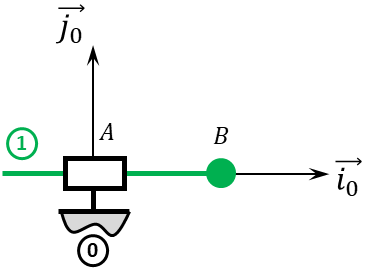
\includegraphics[width=\linewidth]{01_T_01}
\end{marginfigure}
\fi

\question{Tracer le graphe des liaisons.}
\ifprof\begin{marginfigure}
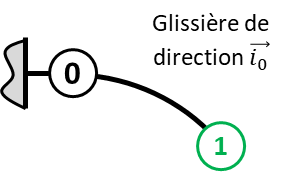
\includegraphics[width=\linewidth]{01_T_01_c}
\end{marginfigure}
\else
\fi


\question{Retracer le schéma cinématique pour $\lambda=\SI{10}{mm}$.}
\ifprof
\begin{marginfigure}
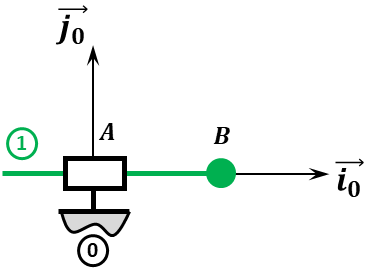
\includegraphics[width=\linewidth]{01_T_02_c}
\end{marginfigure}
\else
\fi

\question{Retracer le schéma cinématique pour $\lambda=-\SI{20}{mm}$.}
\ifprof
\begin{marginfigure}
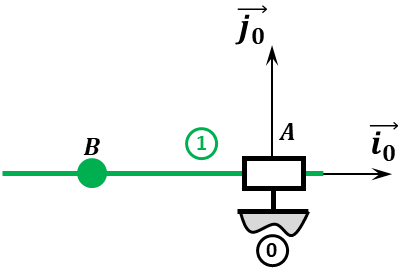
\includegraphics[width=\linewidth]{01_T_03_c}
\end{marginfigure}
\else
\fi

\ifprof
\else
\marginnote{Corrigé  voir \ref{CIN:01:B2:12:01}.}
\fi


 
 
\graphicspath{{\repStyle/png/}{../CIN/CIN-01-ModeliserSchemasCinematiques/02_R/images/}} 
\normaltrue
\correctiontrue

%\UPSTIidClasse{11} % 11 sup, 12 spé
%\newcommand{\UPSTIidClasse}{12}

%\section{Rotation simple} %\label{CIN:01:B2:12:01}
\exer{Mouvement R  $\star$ \label{CIN:01:B2:12:02}}
\setcounter{question}{0}\marginnote{\xpComp{CIN}{01}}%\UPSTIcompetence{B2-12}
\index{Compétence B2-12}\index{Compétence CIN-01}
\index{Mécanisme à 1 rotation}
\ifcorrection
\else
\marginnote{\textbf{Pas de corrigé pour cet exercice.}}
\fi

\ifprof
\else
Soit le mécanisme suivant. On a $\vect{AB}=R\vect{i_1}$ avec $R=\SI{20}{mm}$. 
\begin{marginfigure}
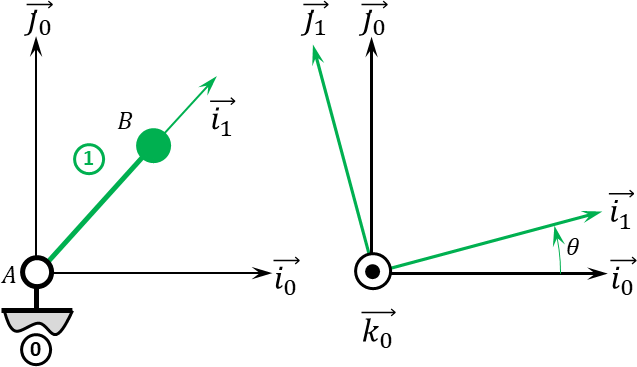
\includegraphics[width=\linewidth]{02_R_01}
\end{marginfigure}
\fi

\ifprof
\begin{multicols}{3}
\else
\fi
\question{Tracer le graphe des liaisons.}
\ifprof
\begin{marginfigure}
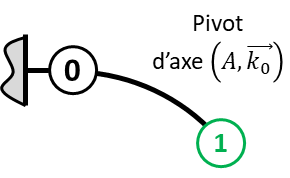
\includegraphics[width=\linewidth]{02_R_01_c}
\end{marginfigure}
\vfill\null
\columnbreak
\else
\fi

\question{Retracer le schéma cinématique pour $\theta=\dfrac{\pi}{4}\,\text{rad}$.}
\ifprof
\begin{marginfigure}
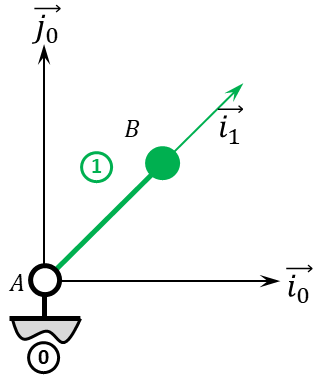
\includegraphics[width=.4\linewidth]{02_R_02_c}
\end{marginfigure}
\vfill\null
\columnbreak
\else
\fi

\question{Retracer le schéma cinématique pour $\theta={\pi}\, \text{rad}$.}
\ifprof
\begin{marginfigure}
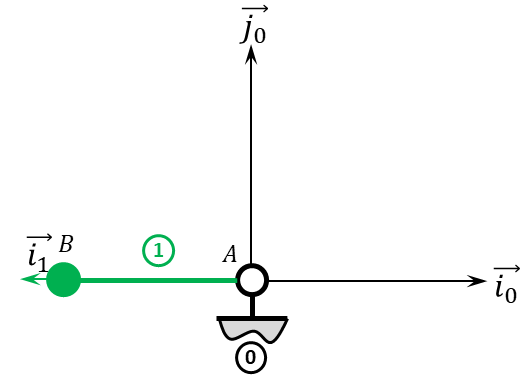
\includegraphics[width=.8\linewidth]{02_R_03_c}
\end{marginfigure}
\else
\fi



\ifprof
\end{multicols}
\else
\fi

\ifprof
\else

\marginnote{Corrigé  voir \ref{CIN:01:B2:12:02}.}

\fi 
 
\graphicspath{{\repStyle/png/}{../CIN/CIN-01-ModeliserSchemasCinematiques/03_TT/images/}} 
\normaltrue
\correctiontrue

%\UPSTIidClasse{11} % 11 sup, 12 spé
%\newcommand{\UPSTIidClasse}{12}


\exer{Mouvement TT -- $\star$ \label{CIN:01:B2:12:03}}
\setcounter{question}{0}\marginnote{\xpComp{CIN}{01}}%\UPSTIcompetence{B2-12}
\index{Compétence B2-12}\index{Compétence CIN-01}
\index{Mécanisme à 2 translations}
\ifcorrection
\else
\marginnote{\textbf{Pas de corrigé pour cet exercice.}}
\fi

\ifprof
\else
Soit le mécanisme suivant. On note $\vect{AB}=\lambda(t)\vect{i_0}$ et $\vect{BC}=\mu(t)\vect{j_0}$.
\begin{marginfigure}
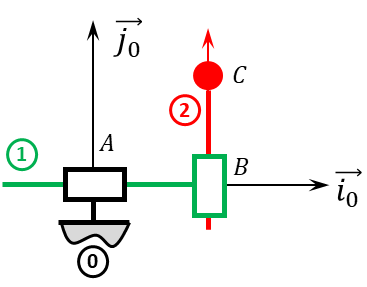
\includegraphics[width=\linewidth]{03_TT_01}
\end{marginfigure}
\fi

\ifprof
\begin{multicols}{3}
\else
\fi
\question{Tracer le graphe des liaisons.}
\ifprof
\begin{marginfigure}
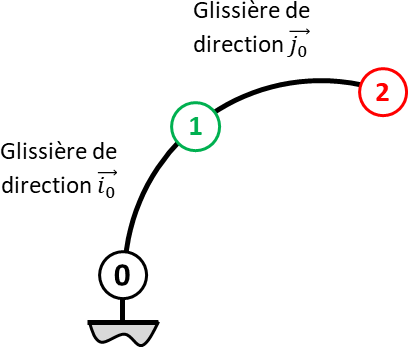
\includegraphics[width=\linewidth]{03_TT_01_c}
\end{marginfigure}
\else
\fi

\question{Retracer le schéma cinématique pour $\lambda=\SI{10}{mm}$ et $\mu=\SI{10}{mm}$.}
\ifprof
\begin{marginfigure}
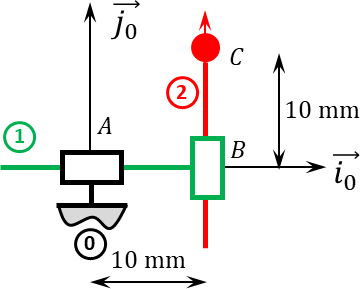
\includegraphics[width=\linewidth]{03_TT_02_c}
\end{marginfigure}
\else
\fi

\question{Retracer le schéma cinématique pour $\lambda=\SI{20}{mm}$ et $\mu=\SI{10}{mm}$.}
\ifprof
\begin{marginfigure}
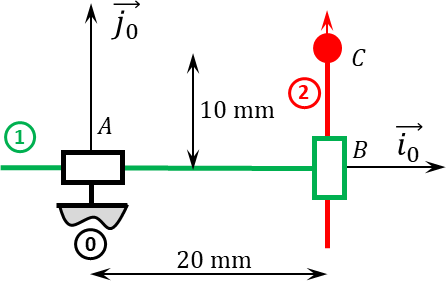
\includegraphics[width=.8\linewidth]{03_TT_03_c}
\end{marginfigure}
\else
\fi


\ifprof
\end{multicols}
\else
\fi

\ifprof
\else

\marginnote{Corrigé  voir \ref{CIN:01:B2:12:03}.}

\fi


 
 
\graphicspath{{\repStyle/png/}{../CIN/CIN-01-ModeliserSchemasCinematiques/04_RR/images/}} 
\normaltrue
\correctiontrue

%\UPSTIidClasse{11} % 11 sup, 12 spé
%\newcommand{\UPSTIidClasse}{12}

\exer{Mouvement RR  $\star$ \label{CIN:01:B2:12:04}}
\setcounter{question}{0}\marginnote{\xpComp{CIN}{01}}%\UPSTIcompetence{B2-12}
\index{Compétence B2-12}\index{Compétence CIN-01}
\index{Mécanisme à 2 rotations}
\ifcorrection
\else
\marginnote{\textbf{Pas de corrigé pour cet exercice.}}
\fi

\ifprof
\else
Soit le mécanisme suivant. On a $\vect{AB}=R\vect{i_1}$ avec $R=\SI{20}{mm}$ et  
$\vect{BC}=L\vect{i_2}$ avec $L=\SI{15}{mm}$.
\begin{marginfigure}
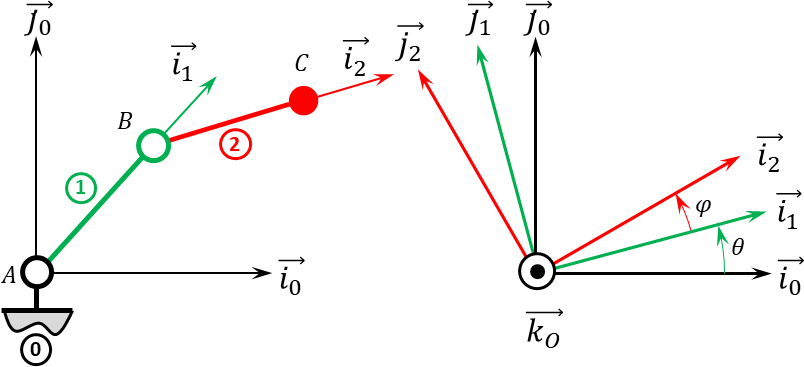
\includegraphics[width=\linewidth]{04_RR_01}
\end{marginfigure}
\fi

\question{Tracer le graphe des liaisons.}
\ifprof
\begin{marginfigure}
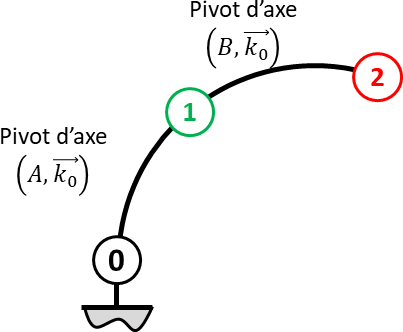
\includegraphics[width=.2\linewidth]{04_RR_01_c}
\end{marginfigure}
\else
\fi


\ifprof
\begin{multicols}{3}
\else
\fi

\question{Retracer le schéma cinématique pour $\theta=\dfrac{\pi}{4}\,\text{rad}$ et $\varphi=\pi\,\text{rad}$.}
\ifprof
\begin{marginfigure}
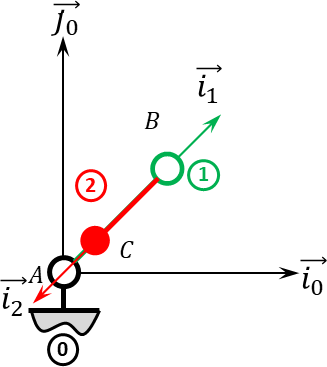
\includegraphics[width=\linewidth]{04_RR_02_c}
\end{marginfigure}
\else
\fi

\question{Retracer le schéma cinématique pour $\theta=\dfrac{\pi}{4}\,\text{rad}$ et $\varphi=-\dfrac{\pi}{4}\,\text{rad}$.}
\ifprof
\begin{marginfigure}
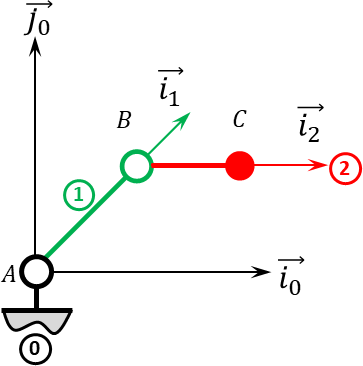
\includegraphics[width=\linewidth]{04_RR_03_c}
\end{marginfigure}
\else
\fi


\question{Retracer le schéma cinématique pour $\theta=\dfrac{3\pi}{4}\,\text{rad}$ et $\varphi=-\dfrac{\pi}{4}\,\text{rad}$.}
\ifprof
\begin{marginfigure}
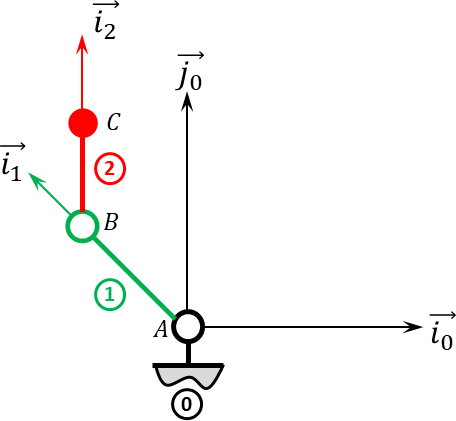
\includegraphics[width=\linewidth]{04_RR_04_c}
\end{marginfigure}
\else
\fi

\ifprof
\end{multicols}
\else
\fi

\ifprof
\else

\marginnote{Corrigé  voir \ref{CIN:01:B2:12:04}.}

\fi 
 
\graphicspath{{\repStyle/png/}{../CIN/CIN-01-ModeliserSchemasCinematiques/05_RT/images/}} 
\normaltrue
\correctiontrue

%\UPSTIidClasse{11} % 11 sup, 12 spé
%\newcommand{\UPSTIidClasse}{12}

\exer{Mouvement RT  $\star$ \label{CIN:01:B2:12:05}}
\setcounter{question}{0}\marginnote{\xpComp{CIN}{01}}%\UPSTIcompetence{B2-12}
\index{Compétence B2-12}\index{Compétence CIN-01}
\index{Mécanisme à 1 rotation et 1 translation}
\ifcorrection
\else
\marginnote{\textbf{Pas de corrigé pour cet exercice.}}
\fi

\ifprof
\else
Soit le mécanisme suivant. On a $\vect{AB}=\lambda(t)\vect{i_1}$.
\begin{marginfigure}
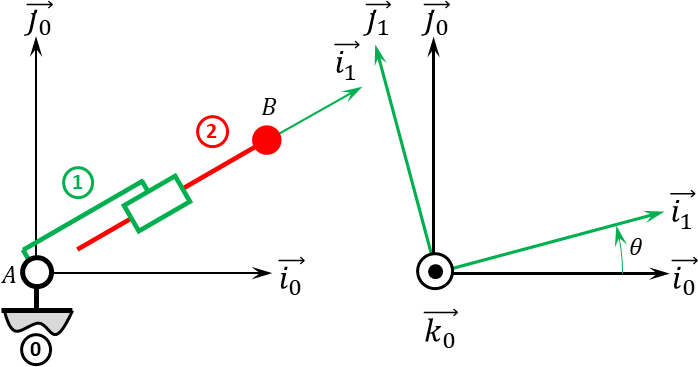
\includegraphics[width=\linewidth]{05_RT_01}
\end{marginfigure}
\fi

\question{Tracer le graphe des liaisons.}
\ifprof
\begin{marginfigure}
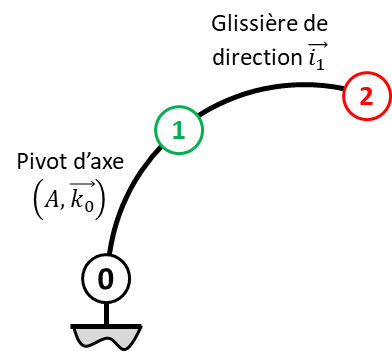
\includegraphics[width=\linewidth]{05_RT_01_01}
\end{marginfigure}
\else
\fi

\question{Retracer le schéma cinématique pour $\theta=\dfrac{\pi}{4}\,\text{rad}$ et $\lambda(t)=\SI{20}{mm}$.}
\ifprof
\else
\fi

\question{Retracer le schéma cinématique pour $\theta=\dfrac{-\pi}{4}\,\text{rad}$ et $\lambda(t)=-\SI{20}{mm}$.}
\ifprof\begin{marginfigure}
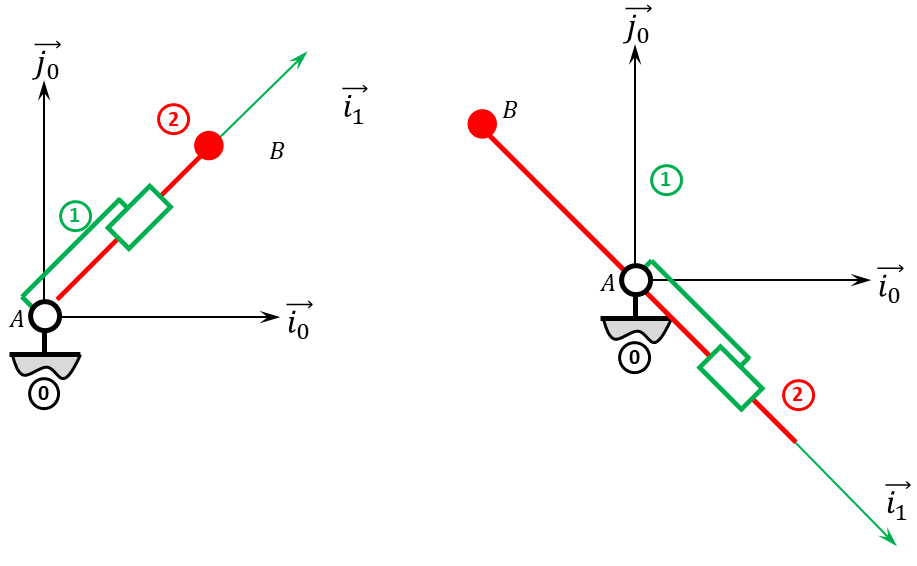
\includegraphics[width=.8\linewidth]{05_RT_01_02}
\end{marginfigure}
\else
\fi




\ifprof
\else

\marginnote{Corrigé  voir \ref{CIN:01:B2:12:05}.}

\fi 
 
\graphicspath{{\repStyle/png/}{../CIN/CIN-01-ModeliserSchemasCinematiques/06_TR/images/}} 
\normaltrue
\correctionfalse

%\UPSTIidClasse{11} % 11 sup, 12 spé
%\newcommand{\UPSTIidClasse}{12}

\exer{Mouvement RT  $\star$ \label{CIN:01:B2:12:06}}
\setcounter{question}{0}\marginnote{\xpComp{CIN}{01}}%\UPSTIcompetence{B2-12}
\index{Compétence B2-12}\index{Compétence CIN-01}
\index{Mécanisme à 1 translation et 1 rotation}
\ifcorrection
\else
\marginnote{\textbf{Pas de corrigé pour cet exercice.}}
\fi

\ifprof
\else
Soit le mécanisme suivant. On a $\vect{AB}=\lambda(t)\vect{i_0}$ et $\vect{BC}=R\vect{i2}$.
\begin{marginfigure}
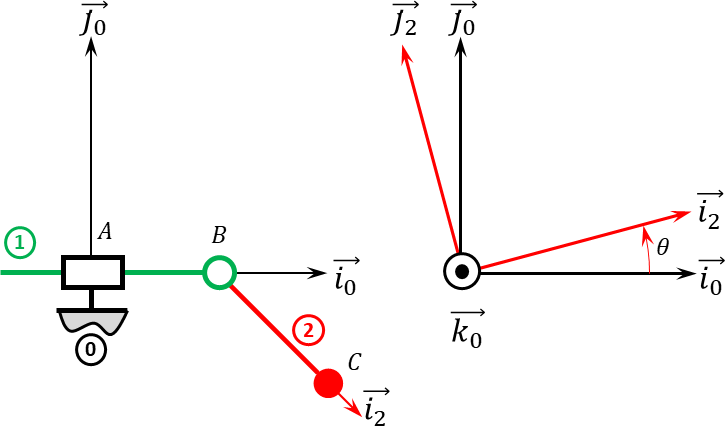
\includegraphics[width=\linewidth]{06_TR_01}
\end{marginfigure}
\fi

\question{Tracer le graphe des liaisons.}
\ifprof
\else
\fi

\question{Retracer le schéma cinématique pour $\theta=\dfrac{\pi}{4}\,\text{rad}$ et $\lambda(t)=\SI{20}{mm}$.}
\ifprof
\else
\fi

\question{Retracer le schéma cinématique pour $\theta=\dfrac{-\pi}{4}\,\text{rad}$ et $\lambda(t)=-\SI{20}{mm}$.}
\ifprof
\else
\fi



\ifprof
\else

\marginnote{Corrigé  voir \ref{CIN:01:B2:12:06}.}

\fi 
 
\graphicspath{{\repStyle/png/}{../CIN/CIN-01-ModeliserSchemasCinematiques/07_RR3D/images/}} 
\normalfalse \difficiletrue \tdifficilefalse
\correctionfalse

%\UPSTIidClasse{11} % 11 sup, 12 spé
%\newcommand{\UPSTIidClasse}{12}

\exer{Mouvement RR 3D  $\star\star$ \label{CIN:01:B2:12:07}}
\setcounter{question}{0}\marginnote{\xpComp{CIN}{01}}%\UPSTIcompetence{B2-12}
\index{Compétence B2-12}\index{Compétence CIN-01}
\index{Mécanisme à 2 rotations 3D}
\ifcorrection
\else
\marginnote{\textbf{Pas de corrigé pour cet exercice.}}
\fi

\ifprof
\else
Soit le mécanisme suivant. On a $\vect{AB}=R\vect{i_1}$ et $\vect{BC}=\ell\vect{i_2}+r\vect{j_2}$. On note $R+\ell=L = \SI{20}{mm}$ et $r=\SI{10}{mm}$.
\begin{marginfigure}
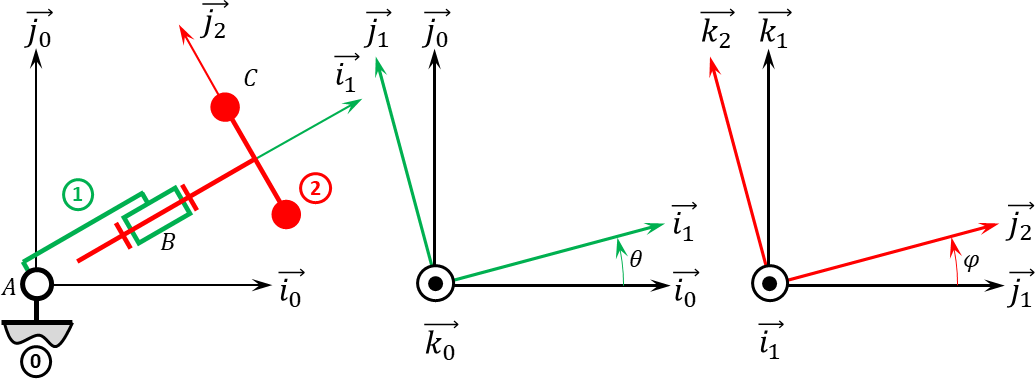
\includegraphics[width=\linewidth]{07_RR3D_01}
\end{marginfigure}
\fi


\question{Tracer le graphe des liaisons.}
\ifprof
\else
\fi

\question{Retracer le schéma cinématique en 3D pour $\theta(t)=\dfrac{\pi}{2}\,\text{rad}$ et $\varphi(t)=\dfrac{\pi}{2}\, \text{rad}$.}
\ifprof
\else
\fi





\ifprof
\else

\marginnote{Corrigé  voir \ref{CIN:01:B2:12:07}.}

\fi 
 
\graphicspath{{\repStyle/png/}{../CIN/CIN-01-ModeliserSchemasCinematiques/08_RR3D/images/}} 
\normalfalse \difficiletrue \tdifficilefalse
\correctionfalse

%\UPSTIidClasse{11} % 11 sup, 12 spé
%\newcommand{\UPSTIidClasse}{12}

\exer{Mouvement RR 3D  $\star\star$ \label{CIN:01:B2:12:08}}
\setcounter{question}{0}\marginnote{\xpComp{CIN}{01}}%\UPSTIcompetence{B2-12}
\index{Compétence B2-12}\index{Compétence CIN-01}
\index{Mécanisme à 2 rotations 3D}
\ifcorrection
\else
\marginnote{\textbf{Pas de corrigé pour cet exercice.}}
\fi

\ifprof
\else
Soit le mécanisme suivant. On a $\vect{AB}=H\vect{j_1}+R\vect{i_1}$ et $\vect{BC}=L\vect{i_2}$. On a $H=\SI{20}{mm}$, $r=\SI{5}{mm}$, $L=\SI{10}{mm}$. 
\begin{marginfigure}
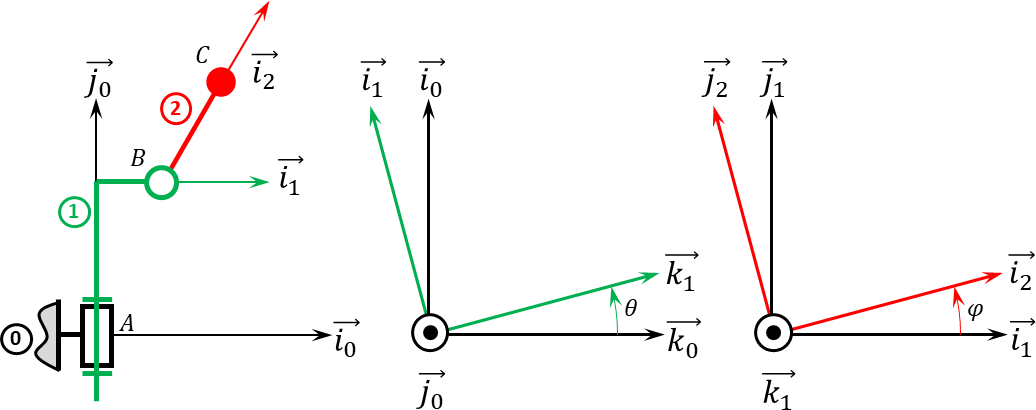
\includegraphics[width=\linewidth]{08_RR3D_01}
\end{marginfigure}
\fi

\question{Tracer le graphe des liaisons.}
\ifprof
\else
\fi

\question{Retracer le schéma cinématique en 3D pour $\theta(t)=\pi\,\text{rad}$ et $\varphi(t)=-\dfrac{\pi}{4}\, \text{rad}$.}
\ifprof
\else
\fi





\ifprof
\else

\marginnote{Corrigé  voir \ref{CIN:01:B2:12:08}.}

\fi 
 
\graphicspath{{\repStyle/png/}{../CIN/CIN-01-ModeliserSchemasCinematiques/09_RT_RSG/images/}} 
\normalfalse \difficiletrue \tdifficilefalse
\correctionfalse

%\UPSTIidClasse{11} % 11 sup, 12 spé
%\newcommand{\UPSTIidClasse}{12}

\exer{Mouvement RT -- RSG  $\star\star$ \label{CIN:01:B2:12:09}}
\setcounter{question}{0}\marginnote{\xpComp{CIN}{01}}%\UPSTIcompetence{B2-12}
\index{Compétence B2-12}\index{Compétence CIN-01}
\index{Mécanisme à 1 rotations, 1 translation et RSG}
\ifcorrection
\else
\marginnote{\textbf{Pas de corrigé pour cet exercice.}}
\fi

\ifprof
\else
Soit le mécanisme suivant. On a $\vect{IA}=R\vect{j_0}$ et $\vect{AB}=\lambda(t)\vect{i_1}$. De plus $R=\SI{15}{mm}$.
\begin{marginfigure}
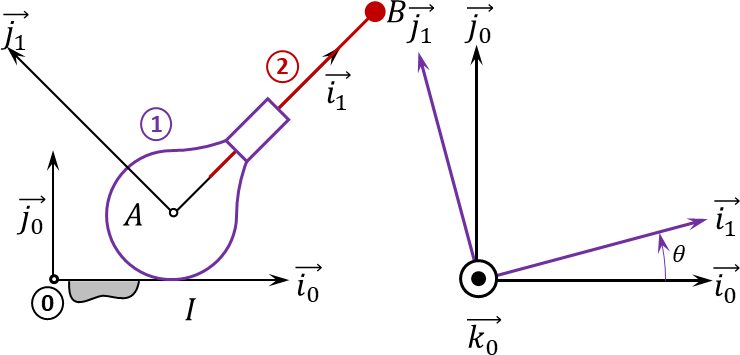
\includegraphics[width=\linewidth]{09_RT_RSG_01}
\end{marginfigure}
\fi


\question{Tracer le graphe des liaisons.}
\ifprof
\else
\fi


\question{Retracer le schéma cinématique pour $\theta(t)=0\,\text{rad}$ et $\lambda(t)=\SI{20}{mm}$. On notera $I_1$ le point de contact entre \textbf{0} et \textbf{1}.}
\ifprof
\else
\fi

\question{Retracer le schéma cinématique pour $\theta(t)=\dfrac{\pi}{2}\,\text{rad}$ et $\lambda(t)=\SI{30}{mm}$. On notera $I_2$ le point de contact entre \textbf{0} et \textbf{1}. On précisera la position des points $I_{0,0}$ et $I_{0,1}$, points résultants de la rupture de contact lors du passage de $\theta(t)$ de 0 à $\dfrac{\pi}{2}$.}
\ifprof
\else
\fi





\ifprof
\else

\marginnote{Corrigé  voir \ref{CIN:01:B2:12:09}.}

\fi 
 
\graphicspath{{\repStyle/png/}{../CIN/CIN-01-ModeliserSchemasCinematiques/1018_BorneReglable/images/}} 
\normalfalse \difficiletrue \tdifficilefalse
\correctionfalse
%\UPSTIidClasse{11} % 11 sup, 12 spé
%\newcommand{\UPSTIidClasse}{12}

\exer{Borne réglable  $\star\star$ \label{CIN:01:B2:12:1018}}
\setcounter{question}{0}\marginnote{\xpComp{CIN}{01}}%\UPSTIcompetence{B2-12}
\index{Compétence B2-12}\index{Compétence CIN-01}
\index{Schéma cinématique}

\ifcorrection
\else
\marginnote{\textbf{Pas de corrigé pour cet exercice.}}
\fi

\ifprof
\else
Soit la borne réglable suivante. 
\begin{marginfigure}
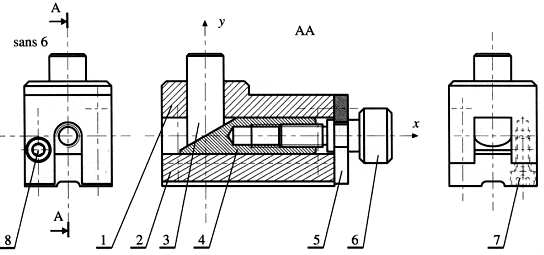
\includegraphics[width=\linewidth]{1018_01}
\end{marginfigure}
\fi


\ifprof
\else
La nomenclature est la suivante. 

\begin{marginfigure}
\begin{tabular}{lll}
\hline
\textbf{Rep} & \textbf{Désignation} & \textbf{Quantité} \\ \hline 
1 & Coulisseau & 1 \\ 
2 & Borne & 1 \\ 
3 & Corps & 1 \\ 
4 & Vis de guidage & 1 \\ 
5 & Couvercle & 1 \\ 
6 & Vis de couvercle & 2 \\ 
7 & Socle & 1 \\ 
8 & Vis de socle & 4 \\ 
10 & Molette & 1 \\ 
12 & Vis & 1 \\
13 & Goupille fendue & 1 \\ 
\hline
\end{tabular}
\end{marginfigure}
\fi


\question{Colorier le dessin de définition en utilisant la même couleur pour une même classe d'équivalence.}
\ifprof
\else
\fi

\question{Lister les classes classes d'équivalence.}
\ifprof
\else
\fi

\question{Donner le graphe de liaisons en précisant rigoureusement les liaisons. Justifier le choix des liaisons.}
\ifprof
\else
\fi


\question{Réaliser le schéma cinématique.}
\ifprof
\else
\fi

\ifprof
\else

\footnotesize
%\begin{marginfigure}
%\begin{tabular}{|p{.9\linewidth}|}
%\hline
%Indications (à vérifier...) :
%\begin{enumerate}
%\item $\vectv{B}{2}{0} = L\varphip(t)\vj{2} +\thetap(t)\left(L\vj{1}-R\vi{0}\right) $.
%\item  $\torseurcin{V}{2}{0} = \torseurl{\vecto{2}{0}=\left( \varphip(t)+\thetap(t) \right) \vk{0} }{ L\varphip(t)\vj{2} +\thetap(t)\left(L\vj{1}-R\vi{0}\right)}{B}$.
%\item $\vectg{B}{2}{0} =  L\varphipp(t)\vj{2}-L\varphip(t)\left(\varphip(t)+\thetap(t) \right)\vi{2}  + \thetapp(t)\left(L\vj{1}-R\vi{0}\right) - L\thetap^2(t)\vi{1}$.
%\end{enumerate} \\ \hline
%\end{tabular}
%\end{marginfigure}
\normalsize



\marginnote{Corrigé  voir \ref{CIN:01:B2:12:1018}.}

\fi 
 
\graphicspath{{\repStyle/png/}{../CIN/CIN-01-ModeliserSchemasCinematiques/1019_RobotPeinture/images/}} 
\normalfalse \difficiletrue \tdifficilefalse
\correctionfalse
%\UPSTIidClasse{11} % 11 sup, 12 spé
%\newcommand{\UPSTIidClasse}{12}

\exer{Robot de toit  $\star\star$ \label{CIN:01:B2:12:1019}}
\setcounter{question}{0}\marginnote{\xpComp{CIN}{01}}%\UPSTIcompetence{B2-12}
\index{Compétence B2-12}\index{Compétence CIN-01}
\index{Schéma cinématique}

\ifcorrection
\else
\marginnote{\textbf{Pas de corrigé pour cet exercice.}}
\fi

\ifprof
\else
Soit le mécanisme donné au verso.
\fi


\ifprof
\else
La nomenclature est la suivante. 
\begin{multicols}{2}
\begin{marginfigure}
\begin{tabular}{|l|l|l|}
\hline
Rep & Nb  & Désignation \\ \hline \hline % & Matière \\ \hline \hline
1 & 1 & Carter inférieur fixe  \\ \hline %&  Al Si 13 \\ \hline 
2&
1&
Carter supérieur pivotant\\ \hline %& Al Si 13 \\ \hline 
3&
2 &
Ecrou hexagonal ISO 4032 - M10 \\ \hline %& \\ \hline 
4&
1&
Rondelle plate ISO 10673 – Type N - 10 \\ \hline %& \\ \hline 
5&
1&
Axe fileté à tête fendu \\ \hline %& \\ \hline 
6&
1&
Plat de fermeture%&
\\ \hline %S 235 \\ \hline 
7&
7&
Rondelle plate ISO 10673 -- Type N - 5 \\ \hline %& \\ \hline 
8&
1&
Bride de liaison support coussinets \\ \hline % &Al Cu 4 Mg Si \\ \hline 
9&
1&
Bride de liaison gauche \\ \hline % & Al Cu 4 Mg Si   \\ \hline 
10&
2&
Coussinet \\ \hline %& Cu Sn 12 P  \\ \hline 
11&
1&
Tube carter \\ \hline %& \\ \hline 
12&
1&
Bride de liaison droite \\ \hline %& Al Cu 4 Mg Si \\ \hline 
13&
1&
Carter cylindrique\\ \hline % & \\ \hline 
14&
1&
Axe excentré \\ \hline %& \\ \hline 
15&
4&
Vis à tête cylindrique à six pans creux\\ \hline % ISO 4762 - M5-50\\ \hline % & \\ \hline 
16&
1&
Chape mâle\\ \hline % & C 45 \\ \hline 
17&
2&
Goupille cylindrique \\ \hline %ISO 8734 - 2x16 \\ \hline %& \\ \hline 
18&
1&
Bielle rotule \\ \hline % &C 45 \\ \hline 
19&
1&
Cale de réglage \\ \hline %& \\ \hline 
20&
1&
Fermeture rotule \\ \hline %& \\ \hline 
21&
1&
Bielle à portée sphérique \\ \hline %& \\ \hline 
22&
3&
Vis à tête cylindrique à six pans creux  \\
&& ISO 4762 - M5-30 \\ \hline %& \\ \hline 
23&
1&
Goupille cylindrique ISO 8734 - 3x30  \\ \hline %& \\ \hline 
24&
1&
Chape femelle \\ \hline %& \\ \hline %C 45 \\ \hline 

25&
1&
Axe de chape \\ \hline % & \\ \hline 
26&
1&
Anneau élastique pour arbre, 4 x 0,4 \\ \hline % & \\ \hline 
27&
2&
Coussinet à collerette \\ \hline %& Cu Sn 12 P \\ \hline 
28&
1&
Bielle \\ \hline % & C 45 \\ \hline 
\end{tabular}
\end{marginfigure}

\begin{marginfigure}
\begin{tabular}{|l|l|l|}
\hline
Rep & Nb  & Désignation \\ \hline \hline % & Matière \\ \hline \hline
29&
3&
Vis à tête cylindrique à six pans creux \\ \hline % ISO 4762 - M5-18 \\ \hline % & \\ \hline 
30&
1&
Axe d'articulation \\ \hline % & \\ \hline 
31&
1&
Axe de sortie \\ \hline % & \\ \hline %100 Cr 6  \\ \hline 
32&
1&
Support d'axe de sortie \\ \hline %C 45 \\ \hline 
33&
1&
Ecrou hexagonal \\ \hline % ISO 4032 - M24  \\ \hline %& \\ \hline 
34&
1&
Rondelle plate \\ \hline % ISO 10673 – Type S - 24\\ \hline % &  \\ \hline 
35&
2&
Coussinet à collerette \\ \hline %& Cu Sn 12 P  \\ \hline 
36&
1&
Plateau support excentrique \\ \hline %& \\ \hline 
37&
1&
Vis à tête moletée \\ \hline %& \\ \hline 
38&
1&
Doigt de réglage \\ \hline % & C 22 \\ \hline 
39&
1&
Coussinet \\ \hline %& Cu Sn 12 P \\ \hline 
40&
1&
Entretoise  \\ \hline 
41&
2&
Anneau élastique pour arbre, 6 x 0,7  \\ \hline %& \\ \hline 
42&
1&
Anneau élastique pour alésage, 32 x 1,5 \\ \hline %& \\ \hline 
43&
1&
Anneau élastique pour arbre, 12 x 1 \\ \hline %& \\ \hline 
44&
1&
Arbre d’entrée \\ \hline %& \\ \hline 
45&
2&
Roulement à une rangée de \\ 
&& billes à contact radial \\ \hline %& \\ \hline 
46&
1&
Support roulements \\ \hline %& Al Cu 4 Mg Si \\ \hline 
47&
1&
Carter \\ \hline % & Al Cu 4 Mg Si \\ \hline 
48&
1&
Vis sans fin Z48 = 2 filets \\ \hline %& \\ \hline 
49&
2&
Boitier\\ \hline % & \\ \hline 
50&
2&
Roulement à une rangée de \\ 
&& billes à contact radial\\  \hline % & \\ \hline 
51&
2&
Joint à deux lèvres \\ \hline %& \\ \hline 
52&
1&
Arbre Creux\\ \hline % & \\ \hline
53&
1&
Vis à tête hexagonale ISO 4014-M6 \\ \hline %  & \\ \hline 
54 & 
1 &
Arbre \\ \hline % & \\ \hline 
55 &
1&
Roue dentée Z55= 60 dents  \\ \hline %&Cu Ni 2 Si  \\ \hline 
\end{tabular}
\end{marginfigure}

\end{multicols}

\fi

\question{Colorier le dessin de définition en utilisant la même couleur pour une même classe d'équivalence.}
\ifprof
\else
\fi

\question{Lister les classes classes d'équivalence.}
\ifprof
\else
\fi

\question{Donner le graphe de liaisons en précisant rigoureusement les liaisons. Justifier le choix des liaisons.}
\ifprof
\else
\fi


\question{Réaliser le schéma cinématique.}
\ifprof
\else
\fi


\ifprof
\else
\begin{marginfigure}
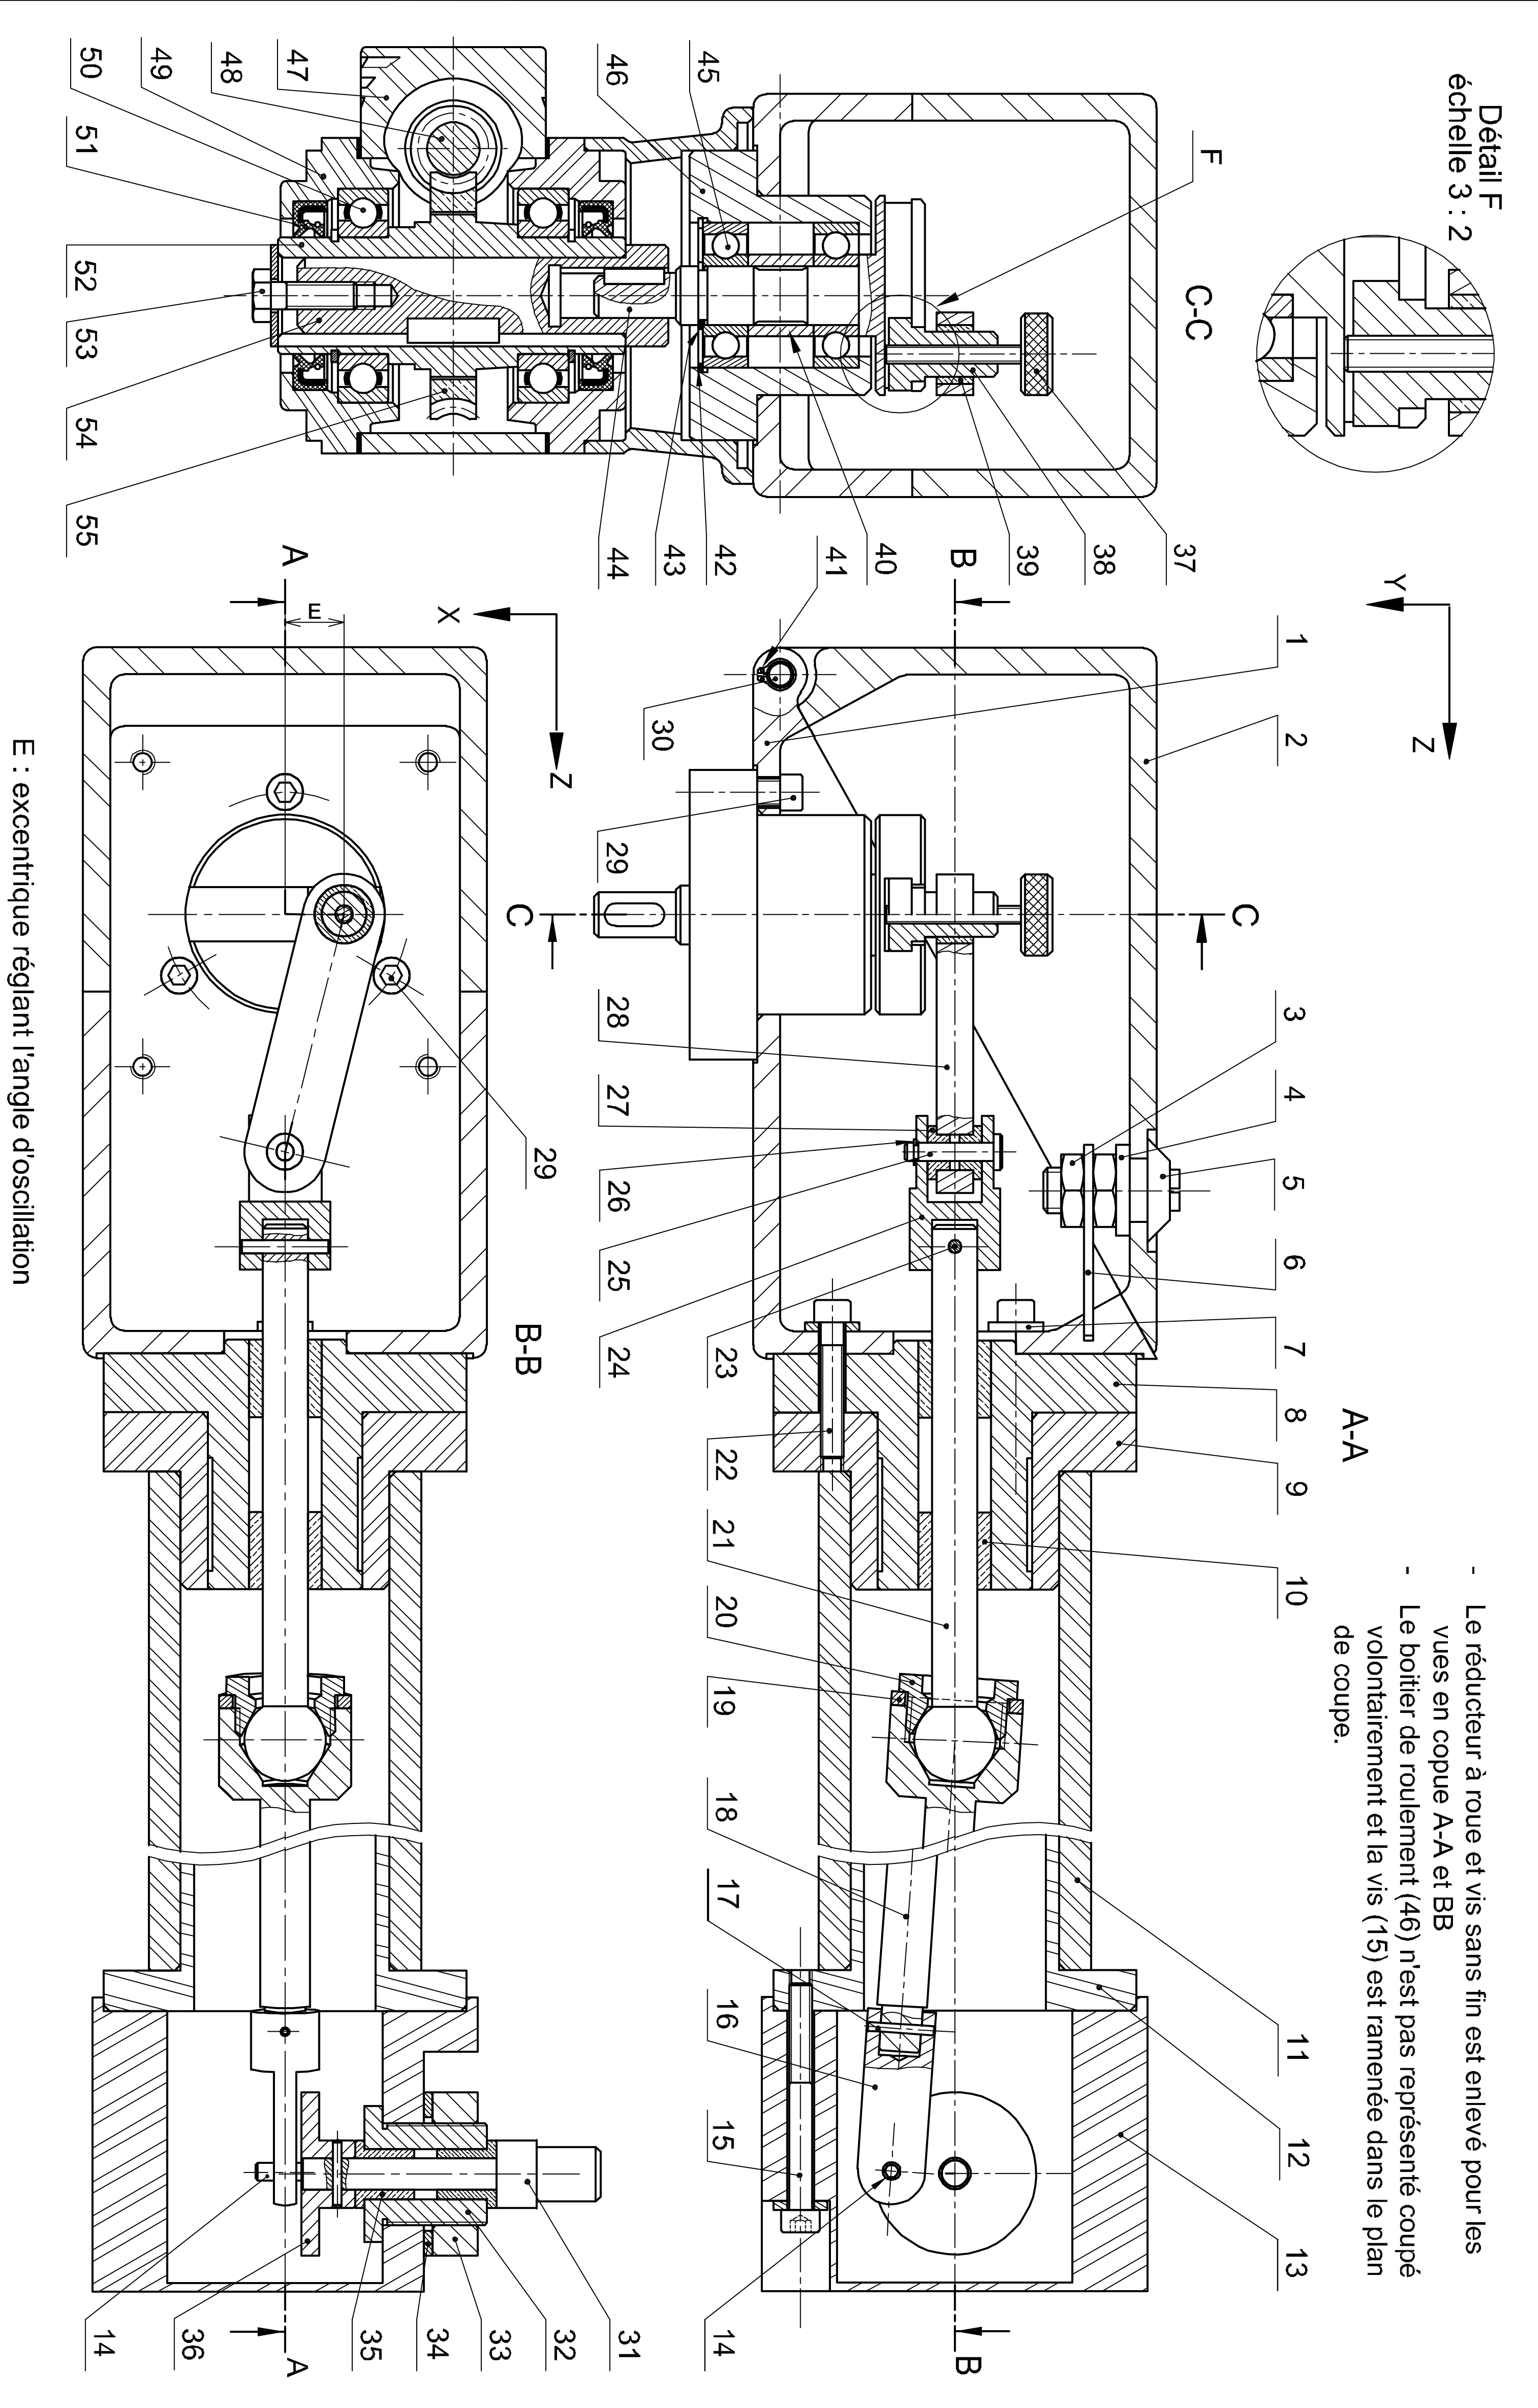
\includegraphics[width=\linewidth]{1019_01}
\end{marginfigure}
\fi


\ifprof
\else

\footnotesize
%\begin{marginfigure}
%\begin{tabular}{|p{.9\linewidth}|}
%\hline
%Indications (à vérifier...) :
%\begin{enumerate}
%\item $\vectv{B}{2}{0} = L\varphip(t)\vj{2} +\thetap(t)\left(L\vj{1}-R\vi{0}\right) $.
%\item  $\torseurcin{V}{2}{0} = \torseurl{\vecto{2}{0}=\left( \varphip(t)+\thetap(t) \right) \vk{0} }{ L\varphip(t)\vj{2} +\thetap(t)\left(L\vj{1}-R\vi{0}\right)}{B}$.
%\item $\vectg{B}{2}{0} =  L\varphipp(t)\vj{2}-L\varphip(t)\left(\varphip(t)+\thetap(t) \right)\vi{2}  + \thetapp(t)\left(L\vj{1}-R\vi{0}\right) - L\thetap^2(t)\vi{1}$.
%\end{enumerate} \\ \hline
%\end{tabular}
%\end{marginfigure}
\normalsize



\marginnote{Corrigé  voir \ref{CIN:01:B2:12:1018}.}

\fi 
 
\graphicspath{{\repStyle/png/}{../CIN/CIN-01-ModeliserSchemasCinematiques/1020_PompeEnsieta/images/}} 
\normalfalse \difficiletrue \tdifficilefalse
\correctionfalse
%\UPSTIidClasse{11} % 11 sup, 12 spé
%\newcommand{\UPSTIidClasse}{12}

\exer{Pompe ENSIETA  $\star\star$ \label{CIN:01:B2:12:1020}}
\setcounter{question}{0}\marginnote{\xpComp{CIN}{01}}%\UPSTIcompetence{B2-12}
\index{Compétence B2-12}\index{Compétence CIN-01}
\index{Schéma cinématique}
\index{Pompe ENSIETA}

\ifcorrection
\else
\marginnote{\textbf{Pas de corrigé pour cet exercice.}}
\fi



\ifprof
\else
Le plan joint format A4 représente l’ensemble monté d’une pompe hydraulique manuelle.

La pompe est fixée sur un support vertical au moyen de 3 trous filetés (1). Une série de trois trous filetés est usinée sur chaque coté du corps (2), permettant ainsi de fixer indifféremment la pompe sur l’une ou l’autre de ses faces.

L’admission de l’huile est effectuée par l’orifice (3), le refoulement par l’orifice (4).

Le pompage s’effectue en actionnant un levier placé dans l’alésage cannelé du maneton (5). Le mouvement alternatif est, par l’intermédiaire de la biellette articulée, transmis au piston coulissant (6).

Lors du mouvement de droite à gauche du piston coulissant, un volume d’huile est aspiré à travers (3) et vient s’emmagasiner dans l’alésage à droite de la tête du piston, simultanément l’huile qui se trouve à gauche de la tête du piston est refoulée par l’orifice (4).

Lors du mouvement de gauche à droite du piston coulissant s’effectue le transfert, à travers de la tête du piston, de l’huile emmagasinée à sa droite (celle-ci passant côté tige). Simultanément une partie de l’huile transférée est refoulée dans (4).

Un clapet anti-retour est constitué d’une bille et d’un ressort. Sur la pompe étudiée ils sont au nombre de trois. 
Le passage du fluide dans un sens, par action sur la bille provoque l’écrasement du ressort et libère le passage. 
Dans le sens contraire l’action du fluide se conjugue avec celle du ressort et interdit le passage. 
\fi

\question{Le diamètre nominal de la bille contenue dans le clapet anti-retour situé sur l’orifice (4) est identique à celui de l’alésage qui la guide. Est-ce fonctionnellement correct ? Justifier votre réponse. L’observation de la pièce (7) du clapet situé sur l’orifice (3) peut vous aider pour la réponse.}

\question{L’alésage du corps contenant l’extrémité du raccord orifice (4) et l’alésage sur lequel le piston (6) coulisse doivent-ils être réalisés avec le même type d’état de surface ? Justifier votre réponse.}

\question{Entre la tige du piston et l’alésage du corps, quel ajustement choisir ? Préciser s’il s’agit d’un ajustement avec jeu, avec serrage ou ajusté.}

\question{D’après la représentation du dessin d’ensemble, un des composants de la pompe ne peut pas être monté. Quel est-il (donner son numéro) ? Pourquoi ? Que faudrait-il faire pour le rendre montable ?}

\question{Dans le mouvement de droite à gauche du piston, le volume aspiré dans (3) à droite de la tête de piston est-il le même que celui refoulé à gauche de la tête de piston dans (4) ? Justifier votre réponse.}


\ifprof
\else
On donne les dimensions suivantes :
\begin{itemize}
\item tête de piston = \SI{29}{mm};
\item tige de piston = \SI{18}{mm};
\item course du piston = \SI{31}{mm}.
\end{itemize}
\fi

\question{Quel est le volume d’huile  envoyé à la sortie (4) :}
\textit{
\begin{itemize}
\item lors de la course droite -- gauche du piston ?
\item lors de la course gauche -- droite du piston ?
\end{itemize}}


\ifprof
\else

\subsection*{Schéma cinématique}
On considère la pompe sans aucun clapet. Seule la transformation de mouvement permettant le déplacement du piston nous intéresse.

\fi

\question{Faire le schéma cinématique de la pompe.}


\ifprof
\else
\begin{marginfigure}
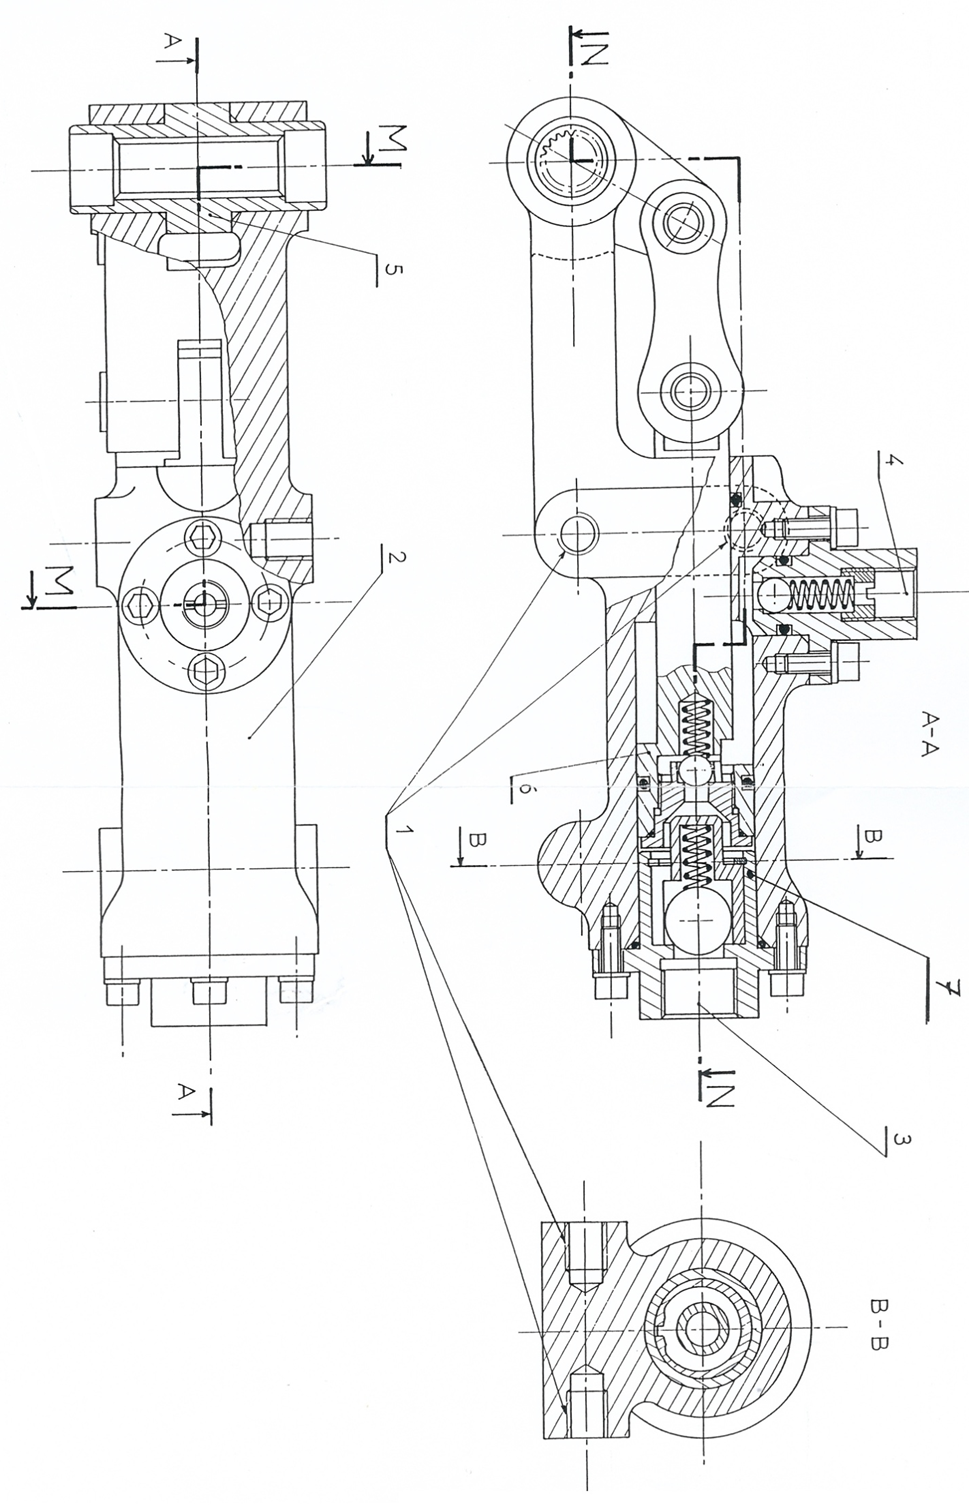
\includegraphics[width=.9\linewidth]{1020_02}
\end{marginfigure}
\fi


\ifprof
\else

\footnotesize
%\begin{marginfigure}
%\begin{tabular}{|p{.9\linewidth}|}
%\hline
%Indications (à vérifier...) :
%\begin{enumerate}
%\item $\vectv{B}{2}{0} = L\varphip(t)\vj{2} +\thetap(t)\left(L\vj{1}-R\vi{0}\right) $.
%\item  $\torseurcin{V}{2}{0} = \torseurl{\vecto{2}{0}=\left( \varphip(t)+\thetap(t) \right) \vk{0} }{ L\varphip(t)\vj{2} +\thetap(t)\left(L\vj{1}-R\vi{0}\right)}{B}$.
%\item $\vectg{B}{2}{0} =  L\varphipp(t)\vj{2}-L\varphip(t)\left(\varphip(t)+\thetap(t) \right)\vi{2}  + \thetapp(t)\left(L\vj{1}-R\vi{0}\right) - L\thetap^2(t)\vi{1}$.
%\end{enumerate} \\ \hline
%\end{tabular}
%\end{marginfigure}
\normalsize



\marginnote{Corrigé  voir \ref{CIN:01:B2:12:1020}.}

\fi 
 
\graphicspath{{\repStyle/png/}{../CIN/CIN-01-ModeliserSchemasCinematiques/10_PompePalette/images/}} 
\normalfalse \difficiletrue \tdifficilefalse
\correctiontrue

%\UPSTIidClasse{11} % 11 sup, 12 spé
%\newcommand{\UPSTIidClasse}{12}

\exer{Pompe à palettes  $\star\star$ \label{CIN:01:B2:12:10}}
\setcounter{question}{0}\marginnote{\xpComp{CIN}{01}}%\UPSTIcompetence{B2-12}
\index{Compétence B2-12}\index{Compétence CIN-01}
\index{Pompe à palettes}
\ifcorrection
\else
\marginnote{\textbf{Pas de corrigé pour cet exercice.}}
\fi

\ifprof
\else
Soit le mécanisme suivant. On a $\vect{AO}=e\vect{i_0}$ et $\vect{AB}=\lambda(t)\vect{i_1}$. De plus $e=\SI{10}{mm}$ et $R=\SI{20}{mm}$. Le contact entre \textbf{0} et \textbf{2} en $B$ est maintenu en permanence (notamment par effet centrifuge lors de la rotation de la pompe).
\begin{marginfigure}
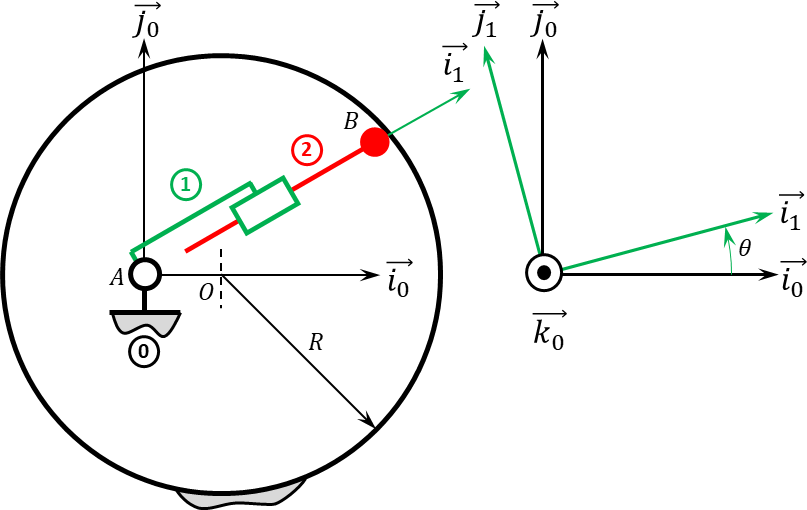
\includegraphics[width=\linewidth]{10_01}
\end{marginfigure}
\fi


\question{Tracer le graphe des liaisons.}
\ifprof
\begin{marginfigure}
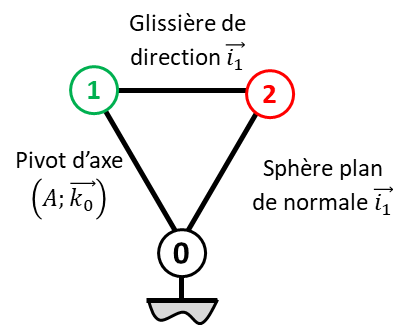
\includegraphics[width=5cm]{10_01_cor}
\end{marginfigure}
\else
\fi


\question{Retracer le schéma cinématique pour $\theta(t)=0 \,\text{rad}$.}
\ifprof
\begin{marginfigure}
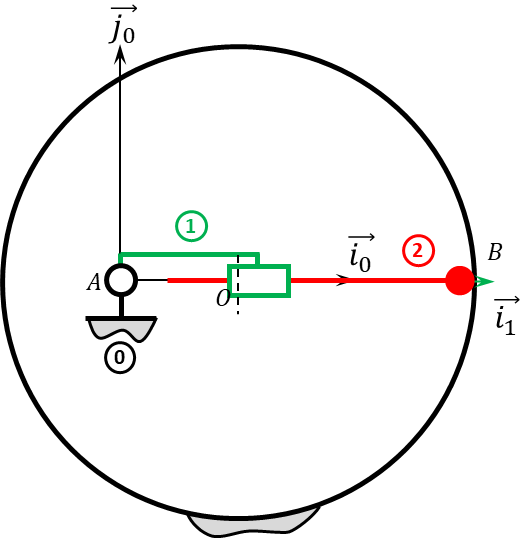
\includegraphics[width=5cm]{10_02_cor}
\end{marginfigure}
\else
\fi

\question{Retracer le schéma cinématique pour $\theta(t)=\pi\,\text{rad}$.}
\ifprof
\begin{marginfigure}
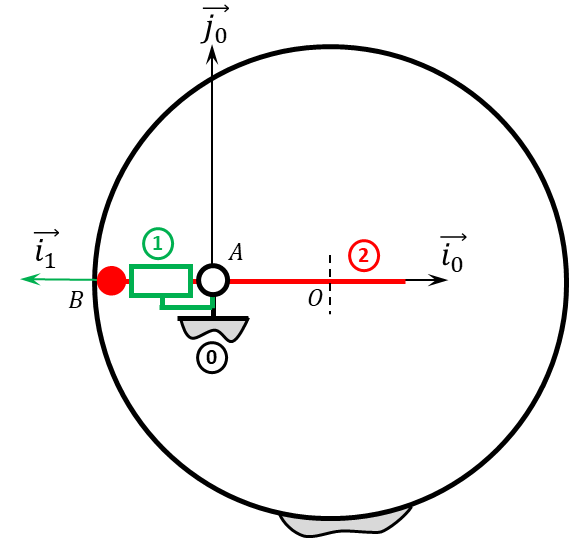
\includegraphics[width=5cm]{10_03_cor}
\end{marginfigure}

\else
\fi


\question{En déduire la course de la pièce \textbf{2}.}
\ifprof
La course de la pièce 2 est donnée par la différence entre la longueur $AB$ maximale et $AB$ minimale : $c= 30-10 = \SI{20}{mm}$.
\else
\fi



\ifprof
\else

\marginnote{Corrigé  voir \ref{CIN:01:B2:12:10}.}

\fi 
 
\graphicspath{{\repStyle/png/}{../CIN/CIN-01-ModeliserSchemasCinematiques/11_PompePistonsRadiaux/images/}} 
\normalfalse \difficiletrue \tdifficilefalse
\correctiontrue

%\UPSTIidClasse{11} % 11 sup, 12 spé
%\newcommand{\UPSTIidClasse}{12}

\exer{Pompe à pistons radiaux  $\star\star$ \label{CIN:01:B2:12:11}}
\setcounter{question}{0}\marginnote{\xpComp{CIN}{01}}%\UPSTIcompetence{B2-12}
\index{Compétence B2-12}\index{Compétence CIN-01}
\index{Pompe à pistons radiaux}
\index{Arbre à cames}
\ifcorrection
\else
\marginnote{\textbf{Pas de corrigé pour cet exercice.}}
\fi

\ifprof
\else
Soit le mécanisme suivant. On a $\vect{AB}=e\vect{i_1}$ et $\vect{BI}=R\vect{j_0}$. De plus, 
$e=\SI{10}{mm}$ et $R=\SI{20}{mm}$. Le contact entre \textbf{1} et \textbf{2} en $B$ est maintenu en permanence par un ressort suffisamment raide (non représenté) positionné entre \textbf{0} et \textbf{2}. 
\begin{marginfigure}
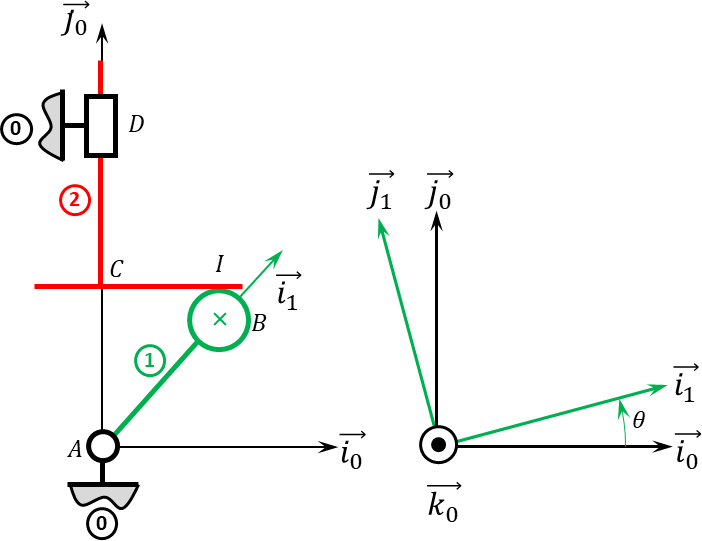
\includegraphics[width=\linewidth]{11_01}
\end{marginfigure}
\fi

\question{Tracer le graphe des liaisons.}
\ifprof
\begin{marginfigure}
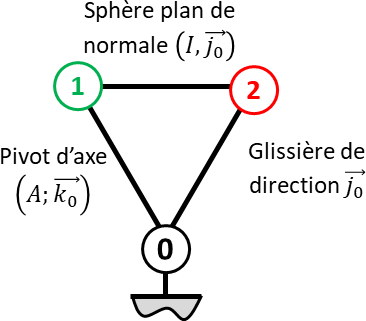
\includegraphics[width=4cm]{11_01_cor}
\end{marginfigure}
\else
\fi

\question{Retracer le schéma cinématique pour $\theta(t)=0 \,\text{rad}$.}
\ifprof
\else
\fi

\question{Retracer le schéma cinématique pour $\theta(t)=\dfrac{\pi}{2}\,\text{rad}$.}
\ifprof
\else
\fi

\question{Retracer le schéma cinématique pour $\theta(t)=-\dfrac{\pi}{2}\,\text{rad}$.}
\ifprof
\begin{marginfigure}
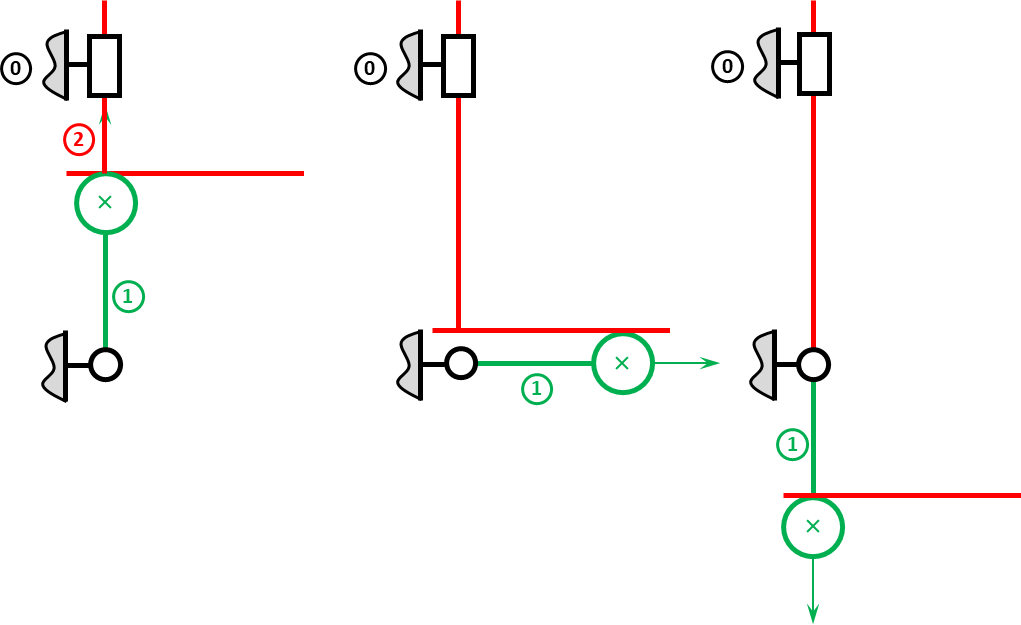
\includegraphics[width=8cm]{11_02_cor}
\end{marginfigure}
\else
\fi


\question{En déduire la course de la pièce \textbf{2}.}
\ifprof
La course est de 
\else
\fi



\ifprof
\else

\marginnote{Corrigé  voir \ref{CIN:01:B2:12:11}.}

\fi 
 
\graphicspath{{\repStyle/png/}{../CIN/CIN-01-ModeliserSchemasCinematiques/12_BielleManivelle/images/}} 
\normalfalse \difficiletrue \tdifficilefalse
\correctionfalse

%\UPSTIidClasse{11} % 11 sup, 12 spé
%\newcommand{\UPSTIidClasse}{12}

\exer{Système bielle manivelle  $\star\star$ \label{CIN:01:B2:12:12}}
\setcounter{question}{0}\marginnote{\xpComp{CIN}{01}}%\UPSTIcompetence{B2-12}
\index{Compétence B2-12}\index{Compétence CIN-01}
\index{Bielle Manivelle}
\index{Moteur}
\ifcorrection
\else
\marginnote{\textbf{Pas de corrigé pour cet exercice.}}
\fi

\ifprof
\else
Soit le mécanisme suivant. On a $\vect{AB}=R\vect{i_1}$ et $\vect{CB}=L\vect{i_2}$. De plus, 
$R=\SI{10}{mm}$ et $L=\SI{20}{mm}$. 

\begin{marginfigure}
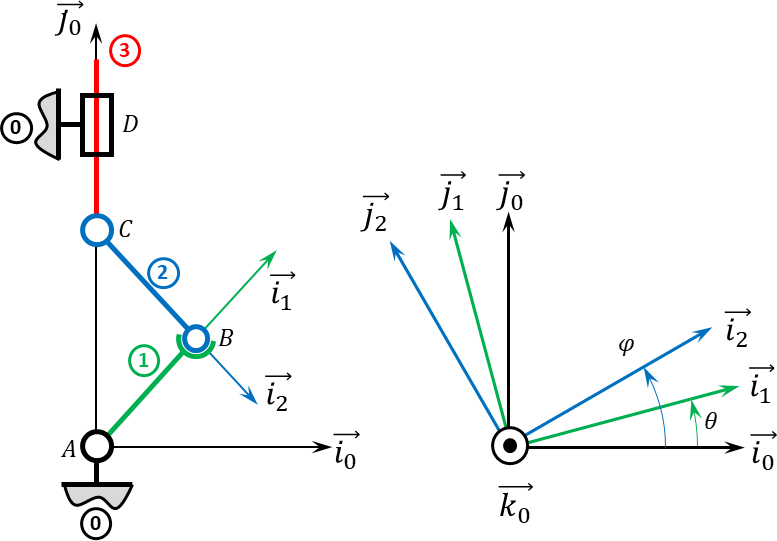
\includegraphics[width=\linewidth]{12_01}
\end{marginfigure}
\fi

\question{Tracer le graphe des liaisons.}
\ifprof
\else
\fi

\question{Retracer le schéma cinématique pour $\theta(t)=\dfrac{\pi}{2}\,\text{rad}$.}
\ifprof
\else
\fi

\question{Retracer le schéma cinématique pour $\theta(t)=-\dfrac{\pi}{2}\,\text{rad}$.}
\ifprof
\else
\fi


\question{En déduire la course de la pièce \textbf{3}.}
\ifprof
\else
\fi



\ifprof
\else
\marginnote{Corrigé  voir \ref{CIN:01:B2:12:12}.}
\fi 
 
\graphicspath{{\repStyle/png/}{../CIN/CIN-01-ModeliserSchemasCinematiques/13_TransfoMouvement/images/}} 
\normalfalse \difficilefalse \tdifficiletrue
\correctionfalse

%\UPSTIidClasse{11} % 11 sup, 12 spé
%\newcommand{\UPSTIidClasse}{12}

\exer{Système de transformation de mouvement  $\star\star$ \label{CIN:01:B2:12:13}}
\setcounter{question}{0}\marginnote{\xpComp{CIN}{01}}%\UPSTIcompetence{B2-12}
\index{Compétence B2-12}\index{Compétence CIN-01}
\index{Bielle Manivelle}
\index{Moteur}
\ifcorrection
\else
\marginnote{\textbf{Pas de corrigé pour cet exercice.}}
\fi

\ifprof
\else
Soit le mécanisme suivant. On a $\vect{AB}=R\vect{i_1}$ et $\vect{CA}=H\vect{j_0}$. De plus, 
$R=\SI{30}{mm}$ et $H=\SI{40}{mm}$. 

\begin{marginfigure}
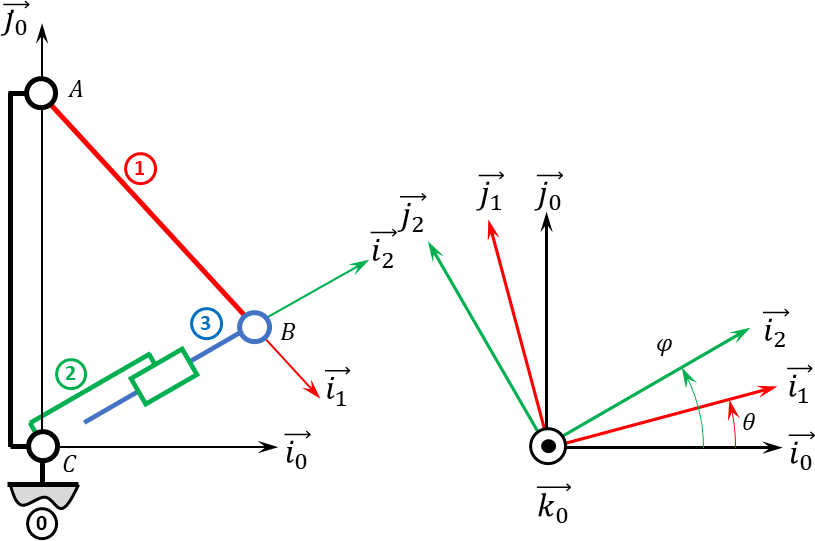
\includegraphics[width=\linewidth]{13_01}
\end{marginfigure}
\fi


\question{Tracer le graphe des liaisons.}
\ifprof
\else
\fi

\question{Retracer le schéma cinématique pour $\theta(t)=\dfrac{\pi}{2}\,\text{rad}$.}
\ifprof
\else
\fi

\question{Retracer le schéma cinématique pour $\theta(t)=0\,\text{rad}$.}
\ifprof
\else
\fi

\question{Retracer le schéma cinématique pour $\theta(t)=-\dfrac{\pi}{2}\,\text{rad}$.}
\ifprof
\else
\fi


\question{En déduire la course de la pièce \textbf{3}.}
\ifprof
\else
\fi



\ifprof
\else

\marginnote{Corrigé  voir \ref{CIN:01:B2:12:13}.}

\fi 
 
\graphicspath{{\repStyle/png/}{../CIN/CIN-01-ModeliserSchemasCinematiques/14_Sympact/images/}} 
\normalfalse \difficiletrue \tdifficilefalse
\correctiontrue

%\UPSTIidClasse{11} % 11 sup, 12 spé
%\newcommand{\UPSTIidClasse}{12}

\exer{Barrière Sympact $\star\star$ \label{CIN:01:B2:12:14}}
\setcounter{question}{0}\marginnote{\xpComp{CIN}{01}}%\UPSTIcompetence{B2-12}
\index{Compétence B2-12}\index{Compétence CIN-01}
\index{Barrière Sympact}
\ifcorrection
\else
\marginnote{\textbf{Pas de corrigé pour cet exercice.}}
\fi

\ifprof
\else
Soit le mécanisme suivant. On a $\vect{AC}=H\vect{j_0}$ et $\vect{CB}=R\vect{i_1}$. De plus, 
$H=\SI{120}{mm}$ et $R=\SI{40}{mm}$. 

\begin{marginfigure}
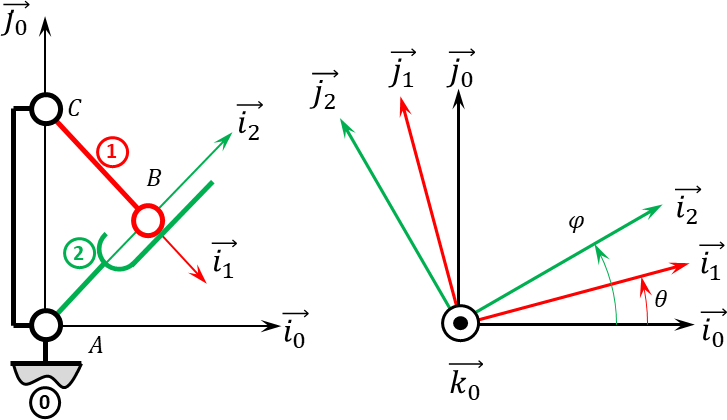
\includegraphics[width=\linewidth]{14_01}
\end{marginfigure}
\fi


\question{Tracer le graphe des liaisons.}
\ifprof
\begin{marginfigure}
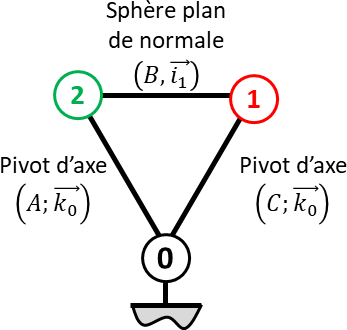
\includegraphics[width=.4\linewidth]{14_02_c}
\end{marginfigure}
\else
\fi

\question{Retracer le schéma cinématique pour $\theta(t)=\dfrac{\pi}{2}\,\text{rad}$.}
\ifprof
\begin{marginfigure}
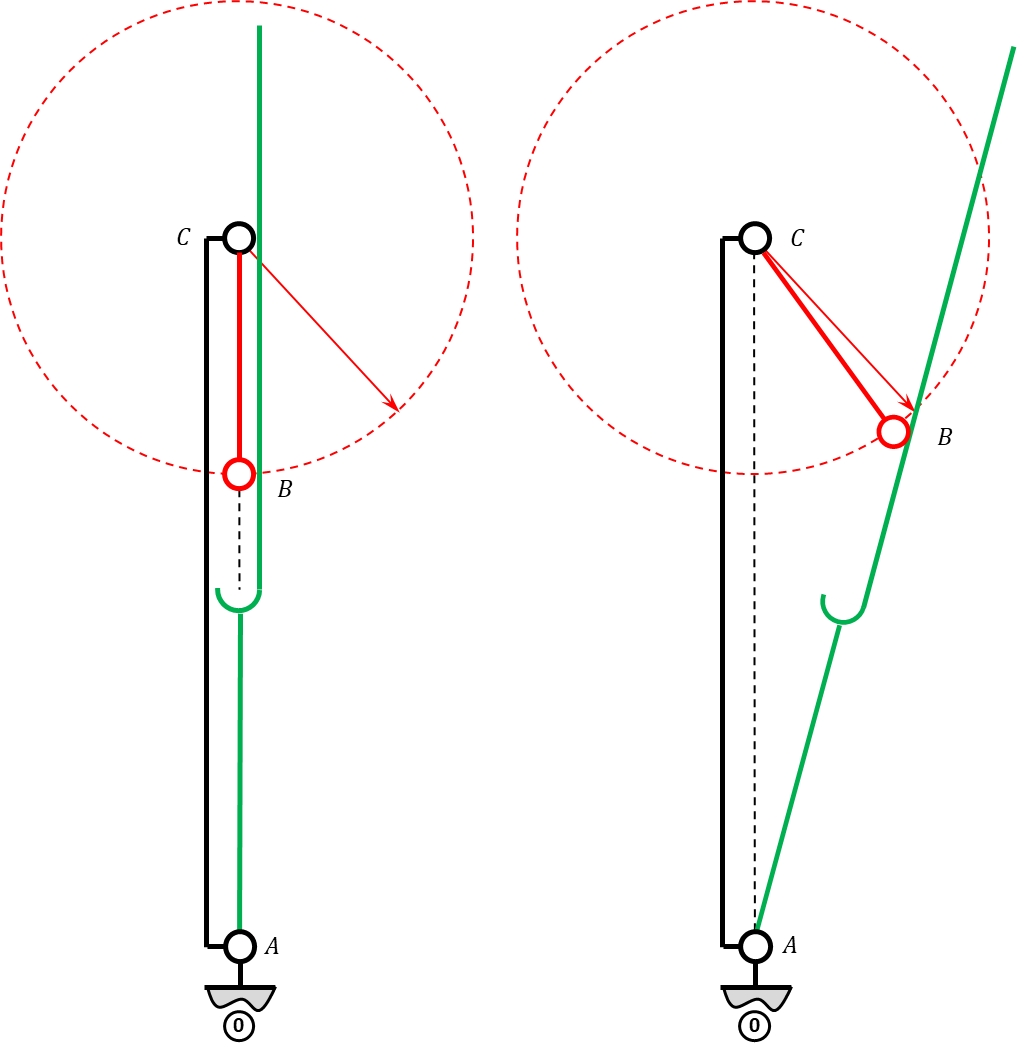
\includegraphics[width=.5\linewidth]{14_01_c}
\end{marginfigure}

\else
\fi

\question{Retracer le schéma cinématique pour $\theta(t)=75\degres$.}
\ifprof
\else
\fi


\question{Dans l'hypothèse où la pièce \textbf{1} peut faire des tours complets, quelle doit être la longueur minimale de la pièce \textbf{2}.}
\ifprof
Dans cas, dans le pire des cas, $A$, $B$ et $C$ sont alignés (avec $B$ au-dessus de $C$). Il faut donc $AB = AC+CB = \SI{160}{mm}$.
\else
\fi

\question{Dans l'hypothèse où la pièce \textbf{2} fait \SI{12}{cm}, quel sera le débattement maximal de la pièce \textbf{1}.}
\ifprof
Comme je suis paresseux, j'ai réalisé la construction avec geogebra. On mesure \SI{160,8}{\degres}.
\begin{marginfigure}
\rotatebox{90}{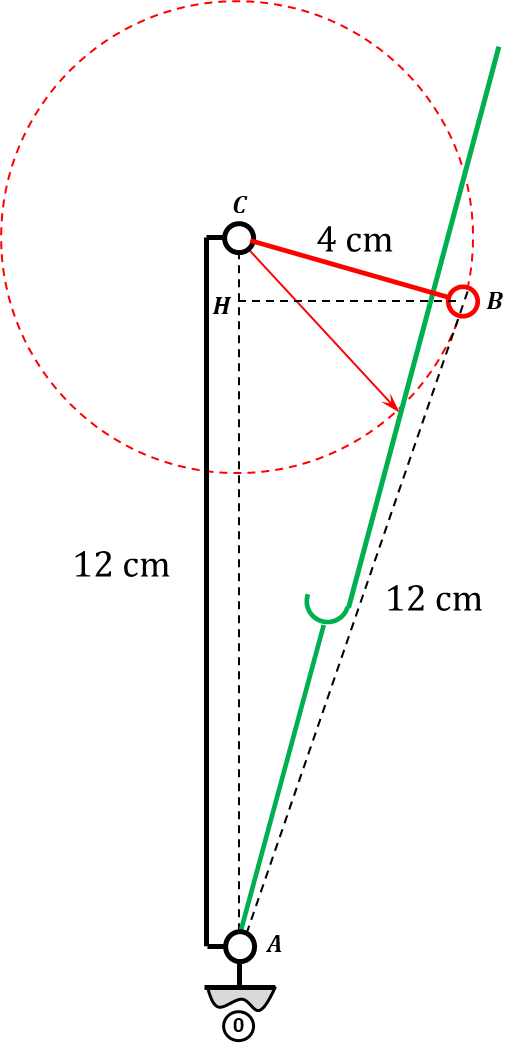
\includegraphics[width=.35\linewidth]{14_03_c}}
\end{marginfigure}
\else
\fi

\ifprof
\else
\ifcolle
\else
\marginnote{
\begin{solution}
\begin{enumerate}
\item .
\item .
\item .
\item \SI{160}{mm}.
\item \SI{160,8}{\degres}.
\end{enumerate}
\end{solution}
\fi
Corrigé  voir \ref{CIN:01:B2:12:14}.}
\fi 
 
\graphicspath{{\repStyle/png/}{../CIN/CIN-01-ModeliserSchemasCinematiques/15_SympactGalet/images/}} 
\normalfalse \difficiletrue \tdifficilefalse
\correctionfalse

%\UPSTIidClasse{11} % 11 sup, 12 spé
%\newcommand{\UPSTIidClasse}{12}

\exer{Barrière Sympact $\star\star$ \label{CIN:01:B2:12:15}}
\setcounter{question}{0}\marginnote{\xpComp{CIN}{01}}%\UPSTIcompetence{B2-12}
\index{Compétence B2-12}\index{Compétence CIN-01}
\index{Barrière Sympact}
\ifcorrection
\else
\marginnote{\textbf{Pas de corrigé pour cet exercice.}}
\fi
\ifprof
\else
Soit le mécanisme suivant. On a $\vect{AC}=H\vect{j_0}$ et $\vect{CB}=R\vect{i_1}$. De plus, 
$H=\SI{120}{mm}$, $R=\SI{40}{mm}$ $BI=\SI{10}{mm}$.

\begin{marginfigure}
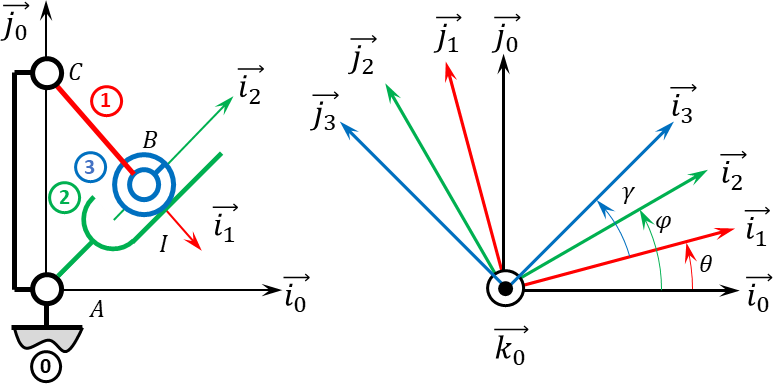
\includegraphics[width=\linewidth]{15_01}
\end{marginfigure}
\fi

\question{Tracer le graphe des liaisons.}
\ifprof
\else
\fi

\question{Retracer le schéma cinématique pour $\theta(t)=\dfrac{\pi}{2}\,\text{rad}$.}
\ifprof
\else
\fi

\question{Retracer le schéma cinématique pour $\theta(t)=-\dfrac{\pi}{2}\,\text{rad}$.}
\ifprof
\else
\fi


%\question{En déduire la course de la pièce \textbf{3}.}
%\ifprof
%\else
%\fi



\ifprof
\else
\marginnote{Corrigé voir \ref{CIN:01:B2:12:15}.}
\fi 
 
\graphicspath{{\repStyle/png/}{../CIN/CIN-01-ModeliserSchemasCinematiques/16_Poussoir/images/}} 
\normalfalse \difficiletrue \tdifficilefalse
\correctionfalse

%\UPSTIidClasse{11} % 11 sup, 12 spé
%\newcommand{\UPSTIidClasse}{12}

\exer{Poussoir $\star\star$ \label{CIN:01:B2:12:16}}
\setcounter{question}{0}\marginnote{\xpComp{CIN}{01}}%\UPSTIcompetence{B2-12}
\index{Compétence B2-12}\index{Compétence CIN-01}
%\index{Barrière Sympact}
\ifcorrection
\else
\marginnote{\textbf{Pas de corrigé pour cet exercice.}}
\fi

\ifprof
\else
Soit le mécanisme suivant. On a $\vect{AC}=L\vect{i_0}+H\vect{j_0}$. De plus, 
$H=\SI{120}{mm}$, $L=\SI{40}{mm}$.

\begin{marginfigure}
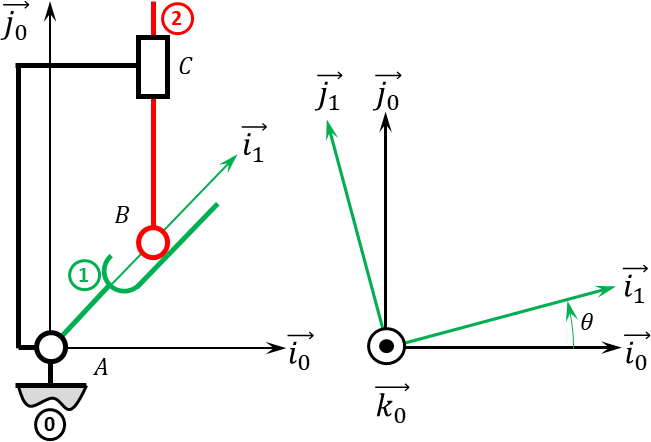
\includegraphics[width=\linewidth]{16_01}
\end{marginfigure}
\fi


\question{Tracer le graphe des liaisons.}
\ifprof
\else
\fi


\question{Retracer le schéma cinématique pour $\theta(t)=\dfrac{\pi}{4}\,\text{rad}$.}
\ifprof
\else
\fi

\question{Retracer le schéma cinématique pour $\theta(t)=-\dfrac{\pi}{4}\,\text{rad}$.}
\ifprof
\else
\fi


%\question{En déduire la course de la pièce \textbf{3}.}
%\ifprof
%\else
%\fi



\ifprof
\else

\marginnote{Corrigé  voir \ref{CIN:01:B2:12:16}.}

\fi 
 
\graphicspath{{\repStyle/png/}{../CIN/CIN-01-ModeliserSchemasCinematiques/17_4Barres/images/}} 
\normalfalse \difficilefalse \tdifficiletrue
\correctionfalse

%\UPSTIidClasse{11} % 11 sup, 12 spé
%\newcommand{\UPSTIidClasse}{12}

\exer{Système 4 barres $\star\star\star$ \label{CIN:01:B2:12:17}} 
\setcounter{question}{0}\marginnote{\xpComp{CIN}{01}}%\UPSTIcompetence{B2-12}
\index{Compétence B2-12}\index{Compétence CIN-01}
\index{Système 4 barres}
\ifcorrection
\else
\marginnote{\textbf{Pas de corrigé pour cet exercice.}}
\fi

\ifprof
\else
On a : 
%\begin{multicols}{2}
\begin{itemize}
\item $\vect{OA} = a \vx{1}-f \vy{1}$ avec $a=\SI{355}{mm}$ et $f=\SI{13}{mm}$;
\item $\vect{AB} = b \vx{2}$ avec $b=\SI{280}{mm}$;
\item $\vect{BC} = -c \vx{3}$ avec $c=\SI{280}{mm}$;
\item $\vect{OC} = -d \vx{0}-e\vy{0}$ avec $d=\SI{89,5}{mm}$ et $e=\SI{160}{mm}$;
\end{itemize}
%\end{multicols}
%a,b,c,d,e,ff = 355,280,280,89.5,160,13

\begin{marginfigure}
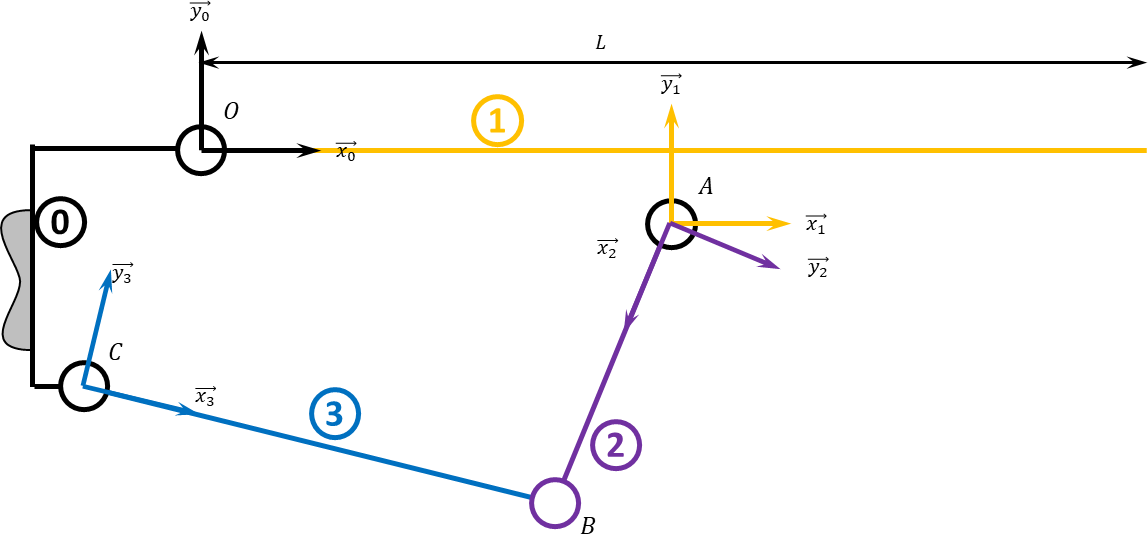
\includegraphics[width=\linewidth]{17_01}

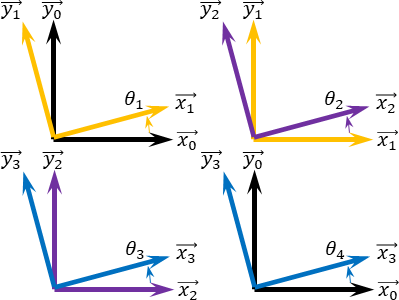
\includegraphics[width=\linewidth]{17_02}
\end{marginfigure}
\fi

\question{Tracer le graphe des liaisons.}
\ifprof
\else
\fi

\question{Retracer le schéma cinématique pour $\theta_1(t)=0\,\text{rad}$.}
\ifprof
\else
\fi

\question{Retracer le schéma cinématique pour $\theta_1(t)=-\dfrac{\pi}{2}\,\text{rad}$.}
\ifprof
\else
\fi


\question{En déduire la course angulaire ($\theta_4$) de la pièce \textbf{3}.}
\ifprof
\else
\fi



\ifprof
\else

\marginnote{Corrigé  voir \ref{CIN:01:B2:12:17}.}

\fi 
 
\graphicspath{{\repStyle/png/}{../CIN/CIN-01-ModeliserSchemasCinematiques/18_Maxpid/images/}} 
\normalfalse \difficilefalse \tdifficiletrue
\correctionfalse

%\UPSTIidClasse{11} % 11 sup, 12 spé
%\newcommand{\UPSTIidClasse}{12}

\exer{Maxpid $\star\star\star$ \label{CIN:01:B2:12:18}}
\setcounter{question}{0}\marginnote{\xpComp{CIN}{01}}%\UPSTIcompetence{B2-12}
\index{Compétence B2-12}\index{Compétence CIN-01}
\index{Maxpid}
\ifcorrection
\else
\marginnote{\textbf{Pas de corrigé pour cet exercice.}}
\fi

\ifprof
\else

Soit le schéma suivant. 
\begin{marginfigure}
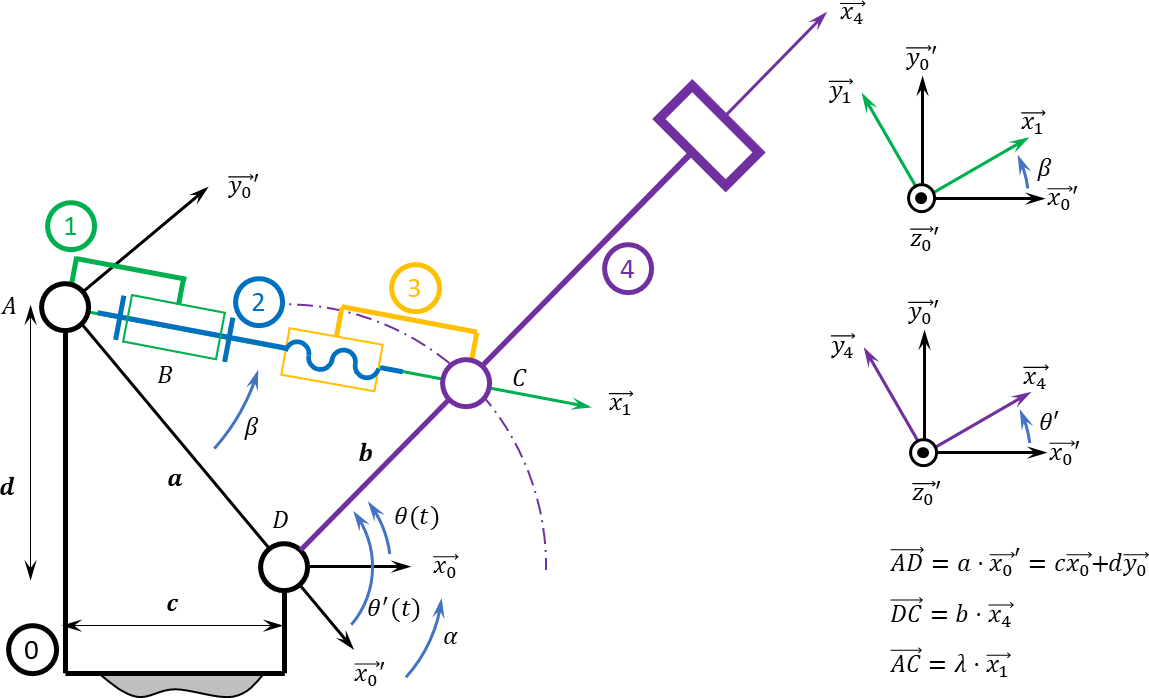
\includegraphics[width=\linewidth]{18_01}
\end{marginfigure}
\fi

Par ailleurs $a=\SI{107,1}{mm}$, $b=\SI{80}{mm}$, $c=\SI{70}{mm}$, $d=\SI{80}{mm}$. Le pas de la vis est de $\SI{4}{mm}$.


\question{Tracer le graphe des liaisons.}
\ifprof
\else
\fi

\question{Retracer le schéma cinématique pour $\theta(t)=0\,\text{rad}$.}
\ifprof
\else
\fi

\question{Retracer le schéma cinématique pour $\theta(t)=\dfrac{\pi}{2}\,\text{rad}$.}
\ifprof
\else
\fi


\question{En déduire la course de $\lambda$.}
\ifprof
\else
\fi



\ifprof
\else

\marginnote{Corrigé  voir \ref{CIN:01:B2:12:18}.}

\fi 
 
\graphicspath{{\repStyle/png/}{../CIN/CIN-01-ModeliserSchemasCinematiques/46_RR_RSG/images/}} 
\normalfalse \difficiletrue \tdifficilefalse
\correctionfalse

%\UPSTIidClasse{11} % 11 sup, 12 spé
%\newcommand{\UPSTIidClasse}{12}

\exer{Mouvement RR -- RSG  $\star\star$ \label{CIN:01:B2:12:46}}
\setcounter{question}{0}\marginnote{\xpComp{CIN}{01}}%\UPSTIcompetence{B2-12}
\index{Compétence B2-12}\index{Compétence CIN-01}
\index{Mécanisme à 1 rotations, 1 translation et RSG}
\ifcorrection
\else
\marginnote{\textbf{Pas de corrigé pour cet exercice.}}
\fi

\ifprof
\else
Soit le mécanisme suivant. On a $\vect{IA}=R\vect{j_0}$ et $\vect{AB}=L\vect{i_1}$. De plus $R=\SI{15}{mm}$.
\begin{marginfigure}
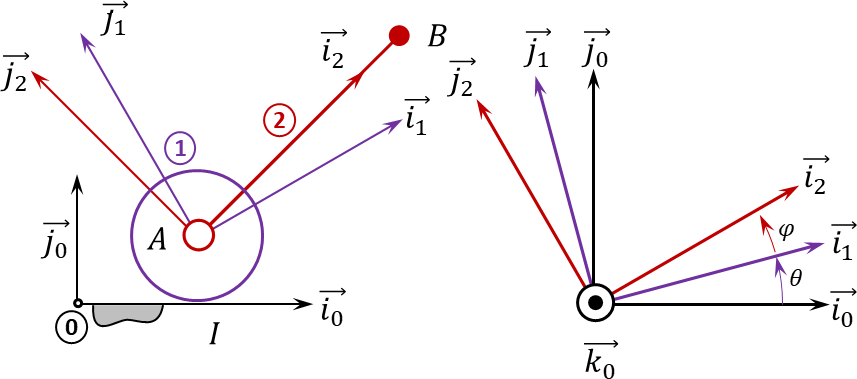
\includegraphics[width=\linewidth]{46_RR_RSG_01}
\end{marginfigure}
\fi


\question{Tracer le graphe des liaisons.}
\ifprof
\else
\fi


\question{Retracer le schéma cinématique pour $\theta(t)=0\,\text{rad}$ et $\varphi(t)=0\,\text{rad}$. On notera $I_0$ le point de contact entre \textbf{0} et \textbf{1}.}
\ifprof
\else
\fi

\question{Retracer le schéma cinématique pour $\theta(t)=\dfrac{\pi}{2}\,\text{rad}$ et $\varphi(t)=0\,\text{rad}$. On notera $I_1$ le point de contact entre \textbf{0} et \textbf{1}. On précisera la position des points $I_{0,0}$ et $I_{0,1}$, points résultants de la rupture de contact lors du passage de $\theta(t)$ de 0 à $\dfrac{\pi}{2}$.}
\ifprof
\else
\fi


\question{Retracer le schéma cinématique pour $\theta(t)=\dfrac{\pi}{2}\,\text{rad}$ et $\varphi(t)=\dfrac{\pi}{2}\,\text{rad}$.} 
\ifprof
\else
\fi


\ifprof
\else

\marginnote{Corrigé  voir \ref{CIN:01:B2:12:46}.}

\fi 
 
\graphicspath{{\repStyle/png/}{../CIN/CIN-01-ModeliserSchemasCinematiques/513_Divers_Tabouret/images/}} 
\normalfalse \difficiletrue \tdifficilefalse
\correctionfalse

%\UPSTIidClasse{11} % 11 sup, 12 spé
%\newcommand{\UPSTIidClasse}{12}

\exer{Tabouret  $\star\star$ \label{CIN:01:B2:12:513}}
\setcounter{question}{0}\marginnote{\xpComp{CIN}{01}}%\UPSTIcompetence{B2-12}
\index{Compétence B2-12}\index{Compétence CIN-01}

\ifcorrection
\else
\marginnote{\textbf{Pas de corrigé pour cet exercice.}}
\fi

\ifprof
\else
\begin{marginfigure}
\centering
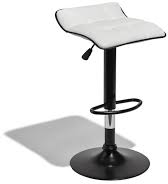
\includegraphics[width=.5\linewidth]{513_01}
\end{marginfigure}
\fi


\question{Proposer un schéma cinématique permettant de modéliser la liaison entre l'assise et le sol.}
\ifprof
\else
\fi

\ifprof
\else

\marginnote{Corrigé  voir \ref{CIN:01:B2:12:513}.}

\fi 
 
\graphicspath{{\repStyle/png/}{../CIN/CIN-01-ModeliserSchemasCinematiques/514_Divers_Tabouret/images/}} 
\normalfalse \difficiletrue \tdifficilefalse
\correctionfalse

%\UPSTIidClasse{11} % 11 sup, 12 spé
%\newcommand{\UPSTIidClasse}{12}

\exer{Tabouret  $\star\star$ \label{CIN:01:B2:12:514}}
\setcounter{question}{0}\marginnote{\xpComp{CIN}{01}}%\UPSTIcompetence{B2-12}
\index{Compétence B2-12}\index{Compétence CIN-01}

\ifcorrection
\else
\marginnote{\textbf{Pas de corrigé pour cet exercice.}}
\fi

\ifprof
\else
\begin{marginfigure}
\centering
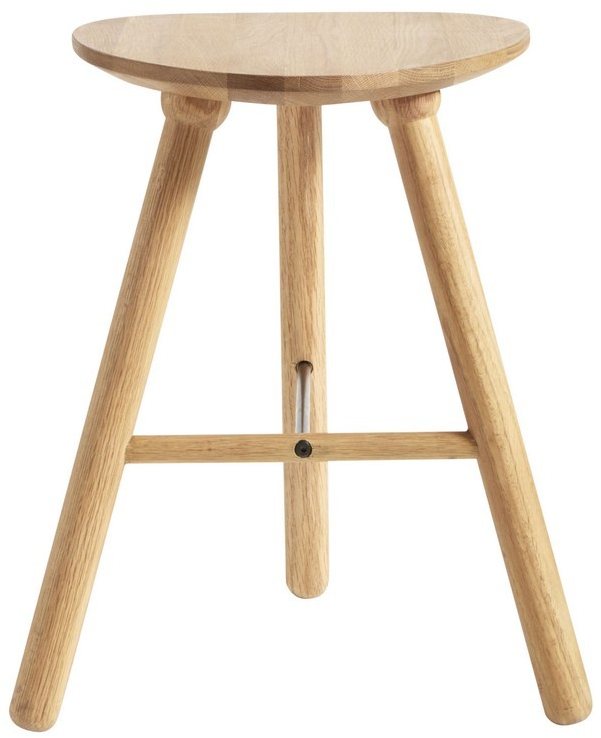
\includegraphics[width=.3\linewidth]{514_01}
\end{marginfigure}
\fi


\question{Proposer 3 schémas cinématiques permettant de modéliser les contacts entre le sol et le tabouret.}
\ifprof
\else
\fi

\ifprof
\else

\marginnote{Corrigé  voir \ref{CIN:01:B2:12:514}.}

\fi 
 
\graphicspath{{\repStyle/png/}{../CIN/CIN-01-Parametrage/01_T/images/}} 
\normaltrue
\correctiontrue

%\UPSTIidClasse{11} % 11 sup, 12 spé
%\newcommand{\UPSTIidClasse}{12}

\exer{Mouvement T -- $\star$ \label{CIN:01:B2:13:PTSI:01}}
\setcounter{question}{0}\marginnote{\xpComp{CIN}{01}}%\UPSTIcompetence[2]{B2-13}
\index{Compétence C2-05}\index{Compétence CIN-01}
\index{Compétence B2-13-PTSI}
\index{Mécanisme à 1 translation}
\ifcorrection
\else
\marginnote{\textbf{Pas de corrigé pour cet exercice.}}
\fi

\ifprof
\else
Soit le mécanisme suivant. 
\begin{marginfigure}
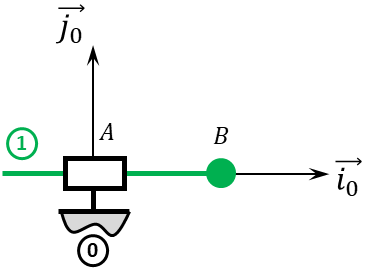
\includegraphics[width=\linewidth]{01_T_01}
\end{marginfigure}
\fi

\question{Réaliser le paramétrage du mécanisme.}
\ifprof~\\
Il n'y a ici que la distance $AB$ à paramétrer. On note $\vect{AB}=\lambda(t)\vi{0}$.
\else
\fi




\ifprof
\else


\marginnote{Corrigé voir \ref{CIN:01:B2:13:PTSI:01}.}

\fi


 
 
\graphicspath{{\repStyle/png/}{../CIN/CIN-01-Parametrage/01_T_02/images/}} 
\normaltrue
\correctionfalse

%\UPSTIidClasse{11} % 11 sup, 12 spé
%\newcommand{\UPSTIidClasse}{12}

\exer{Mouvement T -- $\star$ \label{CIN:01:B2:13:PTSI:01:02}}
\setcounter{question}{0}\marginnote{\xpComp{CIN}{01}}%\UPSTIcompetence[2]{B2-13}
\index{Compétence B2-13-PTSI}
\index{Mécanisme à 1 translation}
\ifcorrection
\else
\marginnote{\textbf{Pas de corrigé pour cet exercice.}}
\fi

\ifprof
\else ~\\
Soit le mécanisme suivant. On note $\vect{AB}=\lambda(t)\vect{i_0}$.
\begin{marginfigure}
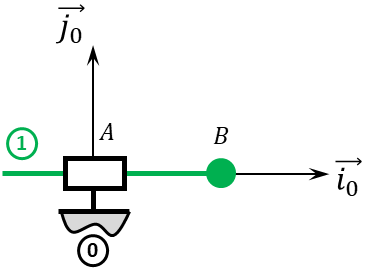
\includegraphics[width=\linewidth]{01_T_01}
\end{marginfigure}
\fi

\question{Réaliser le paramétrage du mécanisme.}
\ifprof ~\\

\else
\fi



\ifprof
\else
\footnotesize

\normalsize

\marginnote{Corrigé voir \ref{CIN:01:B2:13:PTSI:01:02}.}

\fi


 
 
\graphicspath{{\repStyle/png/}{../CIN/CIN-01-Parametrage/02_R/images/}} 
\normaltrue
\correctionfalse

%\UPSTIidClasse{11} % 11 sup, 12 spé
%\newcommand{\UPSTIidClasse}{12}

%\section{Rotation simple} %\label{B2:12:01}
\exer{Mouvement R  $\star$ \label{CIN:01:B2:13:PTSI:02}}
\setcounter{question}{0}\UPSTIcompetence[2]{C2-05}
\marginnote{\xpComp{CIN}{01}}%\UPSTIcompetence[2]{B2-13}
\index{Compétence C2-05}\index{Compétence CIN-01}
\index{Compétence B2-13-PTSI}
\index{Mécanisme à 1 rotation}
\ifcorrection
\else
\marginnote{\textbf{Pas de corrigé pour cet exercice.}}
\fi

\ifprof
\else
Soit le mécanisme suivant. On a $\vect{AB}=R\vect{i_1}$ avec $R=\SI{20}{mm}$. 
\begin{marginfigure}
\includegraphics[width=\linewidth]{02_R_01}
\end{marginfigure}
\fi

\question{Réaliser le paramétrage du mécanisme.}
\ifprof
\else
\fi


\ifprof
\else
\footnotesize

\normalsize

\marginnote{Corrigé voir \ref{CIN:01:B2:13:PTSI:02}.}

\fi 
 
\graphicspath{{\repStyle/png/}{../CIN/CIN-01-Parametrage/02_R_02/images/}} 
\normaltrue
\correctionfalse

%\UPSTIidClasse{11} % 11 sup, 12 spé
%\newcommand{\UPSTIidClasse}{12}

%\section{Rotation simple} %\label{B2:12:01}
\exer{Mouvement R  $\star$ \label{CIN:01:B2:13:PTSI:02}}
\setcounter{question}{0}
\marginnote{\xpComp{CIN}{01}}%\UPSTIcompetence[2]{B2-13}

\index{Compétence B2-13-PTSI}
\index{Mécanisme à 1 rotation}
\ifcorrection
\else
\marginnote{\textbf{Pas de corrigé pour cet exercice.}}
\fi

\ifprof
\else
Soit le mécanisme suivant. 
\begin{marginfigure}
\includegraphics[width=\linewidth]{02_R_01}
\end{marginfigure}
\fi

\question{Réaliser le paramétrage du mécanisme.}
\ifprof ~\\

\else
\fi


\ifprof
\else
\marginnote{Corrigé voir \ref{CIN:01:B2:13:PTSI:02}.}
\fi 
 
\graphicspath{{\repStyle/png/}{../CIN/CIN-01-Parametrage/03_TT/images/}} 
\normaltrue
\correctionfalse

%\UPSTIidClasse{11} % 11 sup, 12 spé
%\newcommand{\UPSTIidClasse}{12}


\exer{Mouvement TT -- $\star$ \label{CIN:01:B2:13:PTSI:03}}
\setcounter{question}{0}\UPSTIcompetence[2]{C2-05}
\marginnote{\xpComp{CIN}{01}}%\UPSTIcompetence[2]{B2-13}
\index{Compétence C2-05}\index{Compétence CIN-01}
\index{Compétence B2-13-PTSI}
\index{Mécanisme à 2 translations}
\ifcorrection
\else
\marginnote{\textbf{Pas de corrigé pour cet exercice.}}
\fi

\ifprof
\else
Soit le mécanisme suivant. 
\begin{marginfigure}
\includegraphics[width=\linewidth]{03_TT_01}
\end{marginfigure}
\fi

\question{Réaliser le paramétrage du mécanisme.}
\ifprof ~\\
\else
\fi




\ifprof
\else
\footnotesize

\normalsize

\marginnote{Corrigé voir \ref{CIN:01:B2:13:PTSI:03}.}

\fi


 
 
\graphicspath{{\repStyle/png/}{../CIN/CIN-01-Parametrage/03_TT_02/images/}} 
\normaltrue
\correctionfalse

%\UPSTIidClasse{11} % 11 sup, 12 spé
%\newcommand{\UPSTIidClasse}{12}


\exer{Mouvement TT -- $\star$ \label{CIN:01:B2:13:PTSI:03:02}}
\setcounter{question}{0}\UPSTIcompetence{B2-13}
\index{Compétence B2-13-PTSI}
\index{Mécanisme à 2 translations}
\ifcorrection
\else
\marginnote{\textbf{Pas de corrigé pour cet exercice.}}
\fi

\ifprof
\else
Soit le mécanisme suivant. 
\begin{marginfigure}
\includegraphics[width=\linewidth]{03_TT_01}
\end{marginfigure}
\fi

\question{Réaliser le paramétrage du mécanisme.}
\ifprof~\\ 

\else
\fi

\ifprof
\else
\footnotesize

\normalsize

\marginnote{Corrigé voir \ref{CIN:01:B2:13:PTSI:03:02}.}

\fi


 
 
\graphicspath{{\repStyle/png/}{../CIN/CIN-01-Parametrage/04_RR/images/}} 
\normaltrue
\correctionfalse

%\UPSTIidClasse{11} % 11 sup, 12 spé
%\newcommand{\UPSTIidClasse}{12}

\exer{Mouvement RR  $\star$ \label{CIN:01:B2:13:PTSI:04}}
\setcounter{question}{0}\UPSTIcompetence[2]{C2-05}
\marginnote{\xpComp{CIN}{01}}%\UPSTIcompetence[2]{B2-13}
\index{Compétence C2-05}\index{Compétence CIN-01}
\index{Compétence B2-13-PTSI}
\index{Mécanisme à 2 rotations}
\ifcorrection
\else
\marginnote{\textbf{Pas de corrigé pour cet exercice.}}
\fi

\ifprof
\else
Soit le mécanisme suivant. 
\begin{marginfigure}
\includegraphics[width=\linewidth]{04_RR_01}
\end{marginfigure}
\fi

\question{Réaliser le paramétrage du mécanisme.}
\ifprof~\\
\else
\fi



\ifprof
\else
\marginnote{Corrigé voir \ref{CIN:01:B2:13:PTSI:04}.}

\fi 
 
\graphicspath{{\repStyle/png/}{../CIN/CIN-01-Parametrage/04_RR_02/images/}} 
\normaltrue
\correctionfalse

%\UPSTIidClasse{11} % 11 sup, 12 spé
%\newcommand{\UPSTIidClasse}{12}

\exer{Mouvement RR  $\star$ \label{CIN:01:B2:13:PTSI:04:02}}
\setcounter{question}{0}\UPSTIcompetence{B2-13}
\index{Compétence B2-13-PTSI}
\index{Mécanisme à 2 rotations}
\ifcorrection
\else
\marginnote{\textbf{Pas de corrigé pour cet exercice.}}
\fi

\ifprof
\else
Soit le mécanisme suivant. 
\begin{marginfigure}
\includegraphics[width=\linewidth]{04_RR_01}
\end{marginfigure}
\fi

\question{Réaliser le paramétrage du mécanisme.}
\ifprof ~\\
\else

\fi



\ifprof
\else
\footnotesize

\normalsize
\marginnote{Corrigé voir \ref{CIN:01:B2:13:PTSI:04:02}.}

\fi 
 
\graphicspath{{\repStyle/png/}{../CIN/CIN-01-Parametrage/05_RT/images/}} 
\normaltrue
\correctionfalse

%\UPSTIidClasse{11} % 11 sup, 12 spé
%\newcommand{\UPSTIidClasse}{12}

\exer{Mouvement RT  $\star$ \label{CIN:01:B2:13:PTSI:05}}
\setcounter{question}{0}\UPSTIcompetence[2]{C2-05}
\marginnote{\xpComp{CIN}{01}\xpComp{GEO}{02}}%\UPSTIcompetence[2]{B2-13}
\index{Compétence C2-05}\index{Compétence CIN-01}
\index{Compétence B2-13-PTSI}
\index{Mécanisme à 1 rotation et 1 translation}
\ifcorrection
\else
\marginnote{\textbf{Pas de corrigé pour cet exercice.}}
\fi

\ifprof
\else
Soit le mécanisme suivant. 
\begin{marginfigure}
\includegraphics[width=\linewidth]{05_RT_01}
\end{marginfigure}
\fi

\question{Réaliser le paramétrage du mécanisme.}
\ifprof
\else
\fi


\ifprof
\else
\marginnote{Corrigé voir \ref{CIN:01:B2:13:PTSI:05}.}

\fi 
 
\graphicspath{{\repStyle/png/}{../CIN/CIN-01-Parametrage/05_RT_02/images/}} 
\normaltrue
\correctionfalse

%\UPSTIidClasse{11} % 11 sup, 12 spé
%\newcommand{\UPSTIidClasse}{12}

\exer{Mouvement RT  $\star$ \label{CIN:01:B2:13:PTSI:05:02}}
\setcounter{question}{0}\UPSTIcompetence{B2-13}
\index{Compétence B2-13-PTSI}
\index{Mécanisme à 1 rotation et 1 translation}
\ifcorrection
\else
\marginnote{\textbf{Pas de corrigé pour cet exercice.}}
\fi

\ifprof
\else
Soit le mécanisme suivant. On a $\vect{AB}=\lambda(t)\vect{i_1}$.
\begin{marginfigure}
\includegraphics[width=\linewidth]{05_RT_01}
\end{marginfigure}
\fi

\question{Réaliser le paramétrage du mécanisme.}
\ifprof  ~\\

\else
\fi



\ifprof
\else
\footnotesize

\normalsize

\marginnote{Corrigé voir \ref{CIN:01:B2:13:PTSI:05:02}.}

\fi 
 
\graphicspath{{\repStyle/png/}{../CIN/CIN-01-Parametrage/06_TR/images/}} 
\normaltrue
\correctionfalse

%\UPSTIidClasse{11} % 11 sup, 12 spé
%\newcommand{\UPSTIidClasse}{12}

\exer{Mouvement RT  $\star$ \label{CIN:01:B2:13:PTSI:06}}
\setcounter{question}{0}\UPSTIcompetence[2]{C2-05}
\marginnote{\xpComp{CIN}{01}}%\UPSTIcompetence[2]{B2-13}
\index{Compétence C2-05}\index{Compétence CIN-01}
\index{Compétence B2-13-PTSI}
\index{Mécanisme à 1 translation et 1 rotation}
\ifcorrection
\else
\marginnote{\textbf{Pas de corrigé pour cet exercice.}}
\fi

\ifprof
\else
Soit le mécanisme suivant. 
\begin{marginfigure}
\includegraphics[width=\linewidth]{06_TR_01}
\end{marginfigure}
\fi

\question{Réaliser le paramétrage du mécanisme.}
\ifprof
\else
\fi

\ifprof
\else
\marginnote{Corrigé voir \ref{CIN:01:B2:13:PTSI:06}.}

\fi 
 
\graphicspath{{\repStyle/png/}{../CIN/CIN-01-Parametrage/06_TR_02/images/}} 
\normaltrue
\correctionfalse

%\UPSTIidClasse{11} % 11 sup, 12 spé
%\newcommand{\UPSTIidClasse}{12}

\exer{Mouvement RT  $\star$ \label{CIN:01:B2:13:PTSI:06:02}}
\setcounter{question}{0}\UPSTIcompetence{B2-13}
\index{Compétence B2-13-PTSI}
\index{Mécanisme à 1 translation et 1 rotation}
\ifcorrection
\else
\marginnote{\textbf{Pas de corrigé pour cet exercice.}}
\fi

\ifprof
\else
Soit le mécanisme suivant. 
\begin{marginfigure}
\includegraphics[width=\linewidth]{06_TR_01}
\end{marginfigure}
\fi

\question{Réaliser le paramétrage du mécanisme.}
\ifprof ~\\

\else
\fi

\ifprof
\else
\footnotesize

\normalsize
\marginnote{Corrigé voir \ref{CIN:01:B2:13:PTSI:06:02}.}

\fi 
 
\graphicspath{{\repStyle/png/}{../CIN/CIN-01-Parametrage/07_RR3D/images/}} 
\normalfalse \difficiletrue \tdifficilefalse
\correctionfalse

%\UPSTIidClasse{11} % 11 sup, 12 spé
%\newcommand{\UPSTIidClasse}{12}

\exer{Mouvement RR 3D  $\star\star$ \label{CIN:01:B2:13:PTSI:07}}
\setcounter{question}{0}\UPSTIcompetence[2]{C2-05}
\marginnote{\xpComp{CIN}{01}}%\UPSTIcompetence[2]{B2-13}
\index{Compétence C2-05}\index{Compétence CIN-01}
\index{Compétence B2-13-PTSI}
\index{Mécanisme à 2 rotations 3D}
\ifcorrection
\else
\marginnote{\textbf{Pas de corrigé pour cet exercice.}}
\fi

\ifprof
\else
Soit le mécanisme suivant. 
\begin{marginfigure}
\includegraphics[width=\linewidth]{07_RR3D_01}
\end{marginfigure}
\fi

\question{Réaliser le paramétrage du mécanisme.}
\ifprof
\else
\fi



\ifprof
\else
\footnotesize

\normalsize

\marginnote{Corrigé voir \ref{CIN:01:B2:13:PTSI:07}.}

\fi 
 
\graphicspath{{\repStyle/png/}{../CIN/CIN-01-Parametrage/07_RR3D_02/images/}} 
\normaltrue \difficilefalse \tdifficilefalse
\correctionfalse

%\UPSTIidClasse{11} % 11 sup, 12 spé
%\newcommand{\UPSTIidClasse}{12}

\exer{Mouvement RR 3D  $\star$ \label{CIN:01:B2:13:PTSI:07:02}}
\setcounter{question}{0}\UPSTIcompetence{B2-13}
\index{Compétence B2-13-PTSI}
\index{Mécanisme à 2 rotations 3D}
\ifcorrection
\else
\marginnote{\textbf{Pas de corrigé pour cet exercice.}}
\fi

\ifprof
\else
Soit le mécanisme suivant. 
\begin{marginfigure}
\includegraphics[width=\linewidth]{07_RR3D_01}
\end{marginfigure}
\fi

\question{Réaliser le paramétrage du mécanisme.}
\ifprof ~\\

\else
\fi





\ifprof
\else
\footnotesize

\normalsize

\marginnote{Corrigé voir \ref{CIN:01:B2:13:PTSI:07}.}

\fi 
 
\graphicspath{{\repStyle/png/}{../CIN/CIN-01-Parametrage/08_RR3D/images/}} 
\normalfalse \difficiletrue \tdifficilefalse
\correctionfalse

%\UPSTIidClasse{11} % 11 sup, 12 spé
%\newcommand{\UPSTIidClasse}{12}

\exer{Mouvement RR 3D  $\star\star$ \label{CIN:01:B2:13:PTSI:08}}
\setcounter{question}{0}\UPSTIcompetence[2]{C2-05}
\marginnote{\xpComp{CIN}{01}}%\UPSTIcompetence[2]{B2-13}
\index{Compétence C2-05}\index{Compétence CIN-01}
\index{Compétence B2-13-PTSI}
\index{Mécanisme à 2 rotations 3D}
\ifcorrection
\else
\marginnote{\textbf{Pas de corrigé pour cet exercice.}}
\fi

\ifprof
\else
Soit le mécanisme suivant. 
\begin{marginfigure}
\includegraphics[width=\linewidth]{08_RR3D_01}
\end{marginfigure}
\fi

\question{Réaliser le paramétrage du mécanisme.}
\ifprof
\else
\fi



\ifprof
\else
\footnotesize

\normalsize
\marginnote{Corrigé voir \ref{CIN:01:B2:13:PTSI:08}.}

\fi 
 
\graphicspath{{\repStyle/png/}{../CIN/CIN-01-Parametrage/08_RR3D_02/images/}} 
\normalfalse \difficiletrue \tdifficilefalse
\correctionfalse

%\UPSTIidClasse{11} % 11 sup, 12 spé
%\newcommand{\UPSTIidClasse}{12}

\exer{Mouvement RR 3D  $\star$ \label{CIN:01:B2:13:PTSI:08}}
\setcounter{question}{0}\marginnote{\xpComp{CIN}{01}}%\UPSTIcompetence[2]{B2-13}
\index{Compétence B2-13-PTSI}
\index{Mécanisme à 2 rotations 3D}
\ifcorrection
\else
\marginnote{\textbf{Pas de corrigé pour cet exercice.}}
\fi

\ifprof
\else
Soit le mécanisme suivant. On a $\vect{AB}=H\vect{j_1}+R\vect{i_1}$ et $\vect{BC}=L\vect{i_2}$. On a $H=\SI{20}{mm}$, $r=\SI{5}{mm}$, $L=\SI{10}{mm}$. 
\begin{marginfigure}
\includegraphics[width=\linewidth]{08_RR3D_01}
\end{marginfigure}
\fi

\question{Réaliser le paramétrage du mécanisme.}
\ifprof
\else
\fi



\ifprof
\else
\footnotesize

\normalsize
\marginnote{Corrigé voir \ref{CIN:01:B2:13:PTSI:08}.}

\fi 
 
\graphicspath{{\repStyle/png/}{../CIN/CIN-01-Parametrage/09_RT_RSG/images/}} 
\normalfalse \difficiletrue \tdifficilefalse
\correctionfalse

%\UPSTIidClasse{11} % 11 sup, 12 spé
%\newcommand{\UPSTIidClasse}{12}

\exer{Mouvement RT -- RSG  $\star\star$ \label{CIN:01:B2:13:PTSI:09}}
\setcounter{question}{0}\marginnote{\xpComp{CIN}{01}}%\UPSTIcompetence[2]{B2-13}
\index{Compétence B2-13-PTSI}
\index{Mécanisme à 1 rotations, 1 translation et RSG}
\ifcorrection
\else
\marginnote{\textbf{Pas de corrigé pour cet exercice.}}
\fi

\ifprof
\else
Soit le mécanisme suivant. 
\begin{marginfigure}
\includegraphics[width=\linewidth]{09_RT_RSG_01}
\end{marginfigure}
\fi


\question{Réaliser le paramétrage du mécanisme.}
\ifprof ~\\

\else
\fi

\question{Donner le torseur cinématique $\torseurcin{V}{2}{0}$ au point $B$.}
\ifprof ~\\
\else
\fi

\question{Déterminer $\vectg{B}{2}{0}$.}
\ifprof ~\\

\else
\fi

\ifprof
\else
\footnotesize

\normalsize
\marginnote{Corrigé voir \ref{CIN:01:B2:13:PTSI:09}.}

\fi 
 
\graphicspath{{\repStyle/png/}{../CIN/CIN-01-Parametrage/10_PompePalette/images/}} 
\normaltrue \difficilefalse \tdifficilefalse
\correctionfalse
%\UPSTIidClasse{11} % 11 sup, 12 spé
%\newcommand{\UPSTIidClasse}{12}

\exer{Pompe à palettes  $\star$ \label{CIN:01:B2:13:PTSI:10}}
\setcounter{question}{0}\marginnote{\xpComp{CIN}{01}}%\UPSTIcompetence[2]{B2-13}
\index{Compétence B2-13-PTSI}
\index{Pompe à palettes}
\ifcorrection
\else
\marginnote{\textbf{Pas de corrigé pour cet exercice.}}
\fi

\ifprof
\else
Soit le mécanisme suivant.
\begin{marginfigure}
\includegraphics[width=.65\linewidth]{10_01}
\end{marginfigure}

\fi


\question{Réaliser le paramétrage du mécanisme.}

\ifprof

\else
\fi


\ifprof
\else
\footnotesize
\ifcolle
\else

\fi

\normalsize
\marginnote{Corrigé voir \ref{CIN:01:B2:13:PTSI:10}.}

\fi 
 
\graphicspath{{\repStyle/png/}{../CIN/CIN-01-Parametrage/11_PompePistonsRadiaux/images/}} 
\normaltrue \difficilefalse \tdifficilefalse
\correctionfalse

%\UPSTIidClasse{11} % 11 sup, 12 spé
%\newcommand{\UPSTIidClasse}{12}

\exer{Pompe à piston axial $\star$ \label{CIN:01:B2:13:PTSI:11}}
\setcounter{question}{0}\marginnote{\xpComp{CIN}{01}}%\UPSTIcompetence[2]{B2-13}
\index{Compétence B2-13-PTSI}
\index{Pompe à piston axial}
\index{Arbre à cames}
\ifcorrection
\else
\marginnote{\textbf{Pas de corrigé pour cet exercice.}}
\fi

\ifprof
\else
Soit le mécanisme suivant. 
\begin{marginfigure}
\includegraphics[width=.6\linewidth]{11_01}
\end{marginfigure}
\fi


\question{Réaliser le paramétrage du mécanisme.}
\ifprof
%$\torseurcin{V}{2}{0} = \torseurl{\vect{0}}{\lambdap (t)\vj{0}}{C}$.
\else
\fi



\ifprof
\else
\footnotesize
\ifcolle
\else

\fi
\normalsize
\marginnote{Corrigé voir \ref{CIN:01:B2:13:PTSI:11}.}

\fi 
 
\graphicspath{{\repStyle/png/}{../CIN/CIN-01-Parametrage/12_BielleManivelle/images/}} 
\normaltrue \difficilefalse \tdifficilefalse
\correctionfalse

%\UPSTIidClasse{11} % 11 sup, 12 spé
%\newcommand{\UPSTIidClasse}{12}

\exer{Système bielle manivelle  $\star$ \label{CIN:01:B2:13:PTSI:12}}
\setcounter{question}{0}\marginnote{\xpComp{CIN}{01}}%\UPSTIcompetence[2]{B2-13}
\index{Compétence B2-13-PTSI}
\index{Bielle Manivelle}
\index{Moteur}
\ifcorrection
\else
\marginnote{\textbf{Pas de corrigé pour cet exercice.}}
\fi

\ifprof
\else
Soit le mécanisme suivant. 

\begin{marginfigure}
\includegraphics[width=0.6\linewidth]{12_01}
\end{marginfigure}
\fi


\question{Réaliser le paramétrage du mécanisme.}
\ifprof

\else
\fi


\ifprof
\else
\marginnote{Corrigé voir \ref{CIN:01:B2:13:PTSI:12}.}

\fi 
 
\graphicspath{{\repStyle/png/}{../CIN/CIN-01-Parametrage/13_TransfoMouvement/images/}} 
\normaltrue \difficilefalse \tdifficilefalse
\correctionfalse

%\UPSTIidClasse{11} % 11 sup, 12 spé
%\newcommand{\UPSTIidClasse}{12}

\exer{Système de transformation de mouvement  $\star$ \label{CIN:01:B2:13:PTSI:13}}
\setcounter{question}{0}\marginnote{\xpComp{CIN}{01}}%\UPSTIcompetence[2]{B2-13}
\index{Compétence B2-13-PTSI}
\index{Bielle Manivelle}
\index{Moteur}
\ifcorrection
\else
\marginnote{\textbf{Pas de corrigé pour cet exercice.}}
\fi

\ifprof
\else
Soit le mécanisme suivant. 
\begin{marginfigure}
\includegraphics[width=.65\linewidth]{13_01}
\end{marginfigure}
\fi


\question{Réaliser le paramétrage du mécanisme.}
\ifprof
\else
\fi

\ifprof
\else
\marginnote{Corrigé voir \ref{CIN:01:B2:13:PTSI:13}.}

\fi 
 
\graphicspath{{\repStyle/png/}{../CIN/CIN-01-Parametrage/14_Sympact/images/}} 
\normalfalse \difficiletrue \tdifficilefalse
\correctionfalse

%\UPSTIidClasse{11} % 11 sup, 12 spé
%\newcommand{\UPSTIidClasse}{12}

\exer{Barrière Sympact $\star\star$ \label{CIN:01:B2:13:PTSI:14}}
\setcounter{question}{0}\UPSTIcompetence{B2-13}
\index{Compétence B2-13-PTSI}
\index{Barrière Sympact}
\ifcorrection
\else
\marginnote{\textbf{Pas de corrigé pour cet exercice.}}
\fi

\ifprof
\else
Soit le mécanisme suivant. 

\begin{marginfigure}
\includegraphics[width=\linewidth]{14_01}
\end{marginfigure}
\fi


\question{Réaliser le paramétrage du mécanisme.}
\ifprof
\else
\fi



\ifprof
\else
\footnotesize
\ifcolle
\else
\fi
\normalsize

\marginnote{Corrigé voir \ref{CIN:01:B2:13:PTSI:14}.}

\fi 
 
\graphicspath{{\repStyle/png/}{../CIN/CIN-01-Parametrage/15_SympactGalet/images/}} 
\normalfalse \difficiletrue \tdifficilefalse
\correctionfalse

%\UPSTIidClasse{11} % 11 sup, 12 spé
%\newcommand{\UPSTIidClasse}{12}

\exer{Barrière Sympact $\star\star$ \label{B2:12:14}}
\setcounter{question}{0}\marginnote{\xpComp{CIN}{01}}%\UPSTIcompetence[2]{B2-13}
\index{Compétence B2-13-PTSI}
\index{Barrière Sympact}
\ifcorrection
\else
\marginnote{\textbf{Pas de corrigé pour cet exercice.}}
\fi
\ifprof
\else
Soit le mécanisme suivant.
\begin{marginfigure}
\includegraphics[width=\linewidth]{15_01}
\end{marginfigure}
\fi



\question{Réaliser le paramétrage du mécanisme.}
\ifprof
\else
\fi


\ifprof
\else
\marginnote{Corrigé voir \ref{CIN:01:B2:12:14}.}

\fi 
 
\graphicspath{{\repStyle/png/}{../CIN/CIN-01-Parametrage/16_Poussoir/images/}} 
\normalfalse \difficiletrue \tdifficilefalse
\correctionfalse

%\UPSTIidClasse{11} % 11 sup, 12 spé
%\newcommand{\UPSTIidClasse}{12}

\exer{Poussoir $\star\star$ \label{B2:12:16}}
\setcounter{question}{0}\UPSTIcompetence{B2-12}
\index{Compétence B2-12}
%\index{Barrière Sympact}
\ifcorrection
\else
\marginnote{\textbf{Pas de corrigé pour cet exercice.}}
\fi

\ifprof
\else
\begin{marginfigure}
\includegraphics[width=\linewidth]{16_01}
\end{marginfigure}
\fi


\question{Réaliser le paramétrage du mécanisme.}
\ifprof
\else
\fi



\ifprof
\else
\marginnote{Corrigé voir \ref{CIN:01:B2:12:16}.}

\fi 
 
\graphicspath{{\repStyle/png/}{../CIN/CIN-01-Parametrage/17_4Barres/images/}} 
\normalfalse \difficilefalse \tdifficiletrue
\correctionfalse

%\UPSTIidClasse{11} % 11 sup, 12 spé
%\newcommand{\UPSTIidClasse}{12}

\exer{Système 4 barres $\star\star\star$ \label{CIN:01:B2:13:PTSI:17}} 
\setcounter{question}{0}\marginnote{\xpComp{CIN}{01}}%\UPSTIcompetence[2]{B2-13}
\index{Compétence B2-13-PTSI}
\index{Système 4 barres}
\ifcorrection
\else
\marginnote{\textbf{Pas de corrigé pour cet exercice.}}
\fi

\ifprof
\else

\begin{marginfigure}
\includegraphics[width=\linewidth]{17_01}
\end{marginfigure}
\fi


\question{Réaliser le paramétrage du mécanisme.}
\ifprof
\else
\fi


\ifprof
\else
\marginnote{Corrigé voir \ref{CIN:01:B2:13:PTSI:17}.}

\fi 
 
\graphicspath{{\repStyle/png/}{../CIN/CIN-01-Parametrage/18_Maxpid/images/}} 
\normalfalse \difficilefalse \tdifficiletrue
\correctionfalse

%\UPSTIidClasse{11} % 11 sup, 12 spé
%\newcommand{\UPSTIidClasse}{12}

\exer{Maxpid $\star\star\star$ \label{CIN:01:B2:13:PTSI:18}}
\setcounter{question}{0}\UPSTIcompetence{B2-13}
\index{Compétence B2-13-PTSI}
\index{Maxpid}
\ifcorrection
\else
\marginnote{\textbf{Pas de corrigé pour cet exercice.}}
\fi

\ifprof
\else

Soit le schéma suivant. 
\begin{marginfigure}
\includegraphics[width=\linewidth]{18_01}
\end{marginfigure}
\fi



\question{Réaliser le paramétrage du mécanisme.}\ifprof
\else
\fi



\ifprof
\else
\marginnote{Corrigé voir \ref{CIN:01:B2:13:PTSI:18}.}

\fi 
 
\graphicspath{{\repStyle/png/}{../CIN/CIN-01-Parametrage/46_RR_RSG/images/}} 
\normalfalse \difficiletrue \tdifficilefalse
\correctionfalse

%\UPSTIidClasse{11} % 11 sup, 12 spé
%\newcommand{\UPSTIidClasse}{12}

\exer{Mouvement RR -- RSG  $\star\star$ \label{CIN:01:B2:13:PTSI:46}}
\setcounter{question}{0}\UPSTIcompetence{B2-13}
\index{Compétence B2-13-PTSI}
\index{Mécanisme à 2 rotations et RSG}
\index{Segway}
\ifcorrection
\else
\marginnote{\textbf{Pas de corrigé pour cet exercice.}}
\fi

\ifprof
\else
Soit le mécanisme suivant.
\begin{marginfigure}
\includegraphics[width=\linewidth]{46_RR_RSG_01}
\end{marginfigure}
\fi


\question{Réaliser le paramétrage du mécanisme.}



\ifprof
\else

\footnotesize

\normalsize


\marginnote{Corrigé voir \ref{CIN:01:B2:13:PTSI:46}.}

\fi 
 
\clearpage 
\newpage 
\section{Déterminer un vecteur vitesse, un torseur cinématique, un vecteur accélération} 
\graphicspath{{\repStyle/png/}{../CIN/CIN-02-VitesseAcceleration/01_T/images/}} 
\normaltrue
\correctiontrue

%\UPSTIidClasse{11} % 11 sup, 12 spé
%\newcommand{\UPSTIidClasse}{12}

\exer{Mouvement T -- $\star$ \label{CIN:02:B2:13:01}}
\setcounter{question}{0}\marginnote{
\xpComp{CIN}{02}}%\xpComp{CIN}{02}%\UPSTIcompetence[2]{C2-05}
%\UPSTIcompetence[2]{B2-13}}

\index{Compétence C2-05}
\index{Compétence B2-13}\index{Compétence CIN-02}
\index{Mécanisme à 1 translation}

\ifcorrection
\else
\marginnote{\marginnote{\textbf{Pas de corrigé pour cet exercice.}}}
\fi

\ifprof
\else
Soit le mécanisme de la figure \ref{fig_01_T:01_T_01}. On note $\vect{AB}=\lambda(t)\vect{i_0}$.
\begin{marginfigure}
\includegraphics[width=\linewidth]{01_T_01}
\caption{\label{fig_01_T:01_T_01} 1 translation}
\end{marginfigure}
\fi

\question{Quel est le mouvement de \textbf{1} par rapport à~\textbf{0}.}
\ifprof~\\
\textbf{1} est en translation de direction $\vi{0}$ par rapport à \textbf{0}.
\else
\fi

\question{Donner l'équation paramétrique de la trajectoire du point $B$, point appartenant à \textbf{1} par rapport à~\textbf{0}.}
\ifprof~\\
On a $\vect{AB}=\lambda(t)\vect{i_0} $. La trajectoire du point $B$ est donc donnée par 
$\left\{ 
\begin{array}{l}
x_B(t) = \lambda (t) \\
y_B(t) = 0 \\
z_B(t) = 0 \\
\end{array}
\right.$ dans le repère $\repere{A}{i_0}{j_0}{z_0}$.
\else
\fi


\ifprof
\else
\marginnote{
\begin{solution}
\begin{enumerate}
\item .
\item $x_B(t) = \lambda (t)$.
\end{enumerate}
\end{solution}}
 
\marginnote{Corrigé  voir \ref{CIN:02:B2:13:01}.}
\fi


 
 
\graphicspath{{\repStyle/png/}{../CIN/CIN-02-VitesseAcceleration/01_T_02/images/}} 
\normaltrue
\correctiontrue

%\UPSTIidClasse{11} % 11 sup, 12 spé
%\newcommand{\UPSTIidClasse}{12}

\exer{Mouvement T -- $\star$ \label{CIN:02:B2:13:01:02}}
\setcounter{question}{0}\marginnote{\xpComp{CIN}{02}}%\marginnote{\UPSTIcompetence[2]{B2-13}}
\index{Compétence B2-13}\index{Compétence CIN-02}
\index{Mécanisme à 1 translation}
\ifcorrection
\else
\marginote{\marginnote{\textbf{Pas de corrigé pour cet exercice.}}}
\fi

\ifprof
\else ~\\
Soit le mécanisme de la figure \ref{fig_01_T_02:01_T_01}. On note $\vect{AB}=\lambda(t)\vect{i_0}$.
\begin{marginfigure}
\includegraphics[width=\linewidth]{01_T_01}
\caption{\label{fig_01_T_02:01_T_01} 1 translation}
\end{marginfigure}
\fi

\question{Donner le torseur cinématique $\torseurcin{V}{1}{0}$ au point $B$.}
\ifprof ~\\
$\torseurcin{V}{1}{0} = \torseurl{\vect{0}}{\dot{\lambda}(t)\vi{0}}{\forall P}$.

$\vectv{B}{1}{0} = \deriv{\vect{AB}}{\rep{0}}=\dot{\lambda}(t)\vi{0}$.
\else
\fi

\question{Déterminer $\vectg{B}{1}{0}$.}
\ifprof  ~\\
 $\vectg{B}{1}{0} = \deriv{\vectv{B}{1}{0}}{\rep{0}}=\ddot{\lambda}(t)\vi{0}$.
\else
\fi


\ifprof
\else
\marginnote{
\begin{solution}
\begin{enumerate}
\item $\torseurcin{V}{1}{0} = \torseurl{\vect{0}}{\dot{\lambda}(t)\vi{0}}{\forall P}$.
\item  $\vectg{B}{1}{0} =\ddot{\lambda}(t)\vi{0}$.
\end{enumerate} 
\end{solution}}

\marginnote{Corrigé  voir \ref{CIN:02:B2:13:01:02}.}
\fi


 
 
\graphicspath{{\repStyle/png/}{../CIN/CIN-02-VitesseAcceleration/02_R/images/}} 
\normaltrue
\correctiontrue

%\UPSTIidClasse{11} % 11 sup, 12 spé
%\newcommand{\UPSTIidClasse}{12}

%\section{Rotation simple} %\label{B2:12:01}
\exer{Mouvement R  $\star$ \label{CIN:02:B2:13:02}}
\setcounter{question}{0}\marginnote{\xpComp{CIN}{02}}%%\xpComp{CIN}{02}%\UPSTIcompetence[2]{C2-05}}
%\marginnote{\xpComp{CIN}{02}}%\marginnote{\UPSTIcompetence[2]{B2-13}}
\index{Compétence C2-05}
\index{Compétence B2-13}\index{Compétence CIN-02}
\index{Mécanisme à 1 rotation}
\ifcorrection
\else
\marginnote{\textbf{Pas de corrigé pour cet exercice.}}
\fi

\ifprof
\else
Soit le mécanisme suivant. On a $\vect{AB}=R\vect{i_1}$ avec $R=\SI{20}{mm}$. 
\begin{marginfigure}
\includegraphics[width=\linewidth]{02_R_01}
\end{marginfigure}
\fi

% ==================
\ifprof
\else
\marginnote{
\begin{solution}
\begin{enumerate}
\item .
\item .
\item $x_B(t) = R\cos\theta (t)$ et $y_B(t) = R\sin\theta (t)$.
\end{enumerate}
\end{solution}
Corrigé  voir \ref{CIN:02:B2:13:02}.}
\fi
% ==================
\question{Quel est le mouvement de \textbf{1} par rapport à~\textbf{0}.}
\ifprof
\textbf{1} est en rotation de centre $A$ et d'axe $\vk{0}$ par rapport à \textbf{0}.
\else
\fi

\question{Quelle est la trajectoire du point $B$ appartenant à \textbf{1} par rapport à~\textbf{0}.}
\ifprof
$B$ est est en rotation par rapport à \textbf{0} (cercle de centre $A$ et de rayon $R$).
\else
\fi

\question{Donner l'équation paramétrique de la trajectoire du point $B$, point appartenant à \textbf{1} par rapport à~\textbf{0}.}
\ifprof

On a $\vect{AB}=R\vi{1}$ $=R\cos\theta \vi{0}+R\sin\theta \vj{0}$. La trajectoire du point $B$ est donc donnée par 
$\left\{ 
\begin{array}{l}
x_B(t) = R\cos\theta (t) \\
y_B(t) = R\sin\theta (t) \\
z_B(t)=0 
\end{array}
\right.$ dans le repère $\repere{A}{i_0}{j_0}{z_0}$.

\else
\fi

 
 
\graphicspath{{\repStyle/png/}{../CIN/CIN-02-VitesseAcceleration/02_R_02/images/}} 
\normaltrue
\correctiontrue

%\UPSTIidClasse{11} % 11 sup, 12 spé
%\newcommand{\UPSTIidClasse}{12}

%\section{Rotation simple} %\label{B2:12:01}
\exer{Mouvement R  $\star$ \label{CIN:02:B2:13:02}}
\setcounter{question}{0}
\marginnote{\xpComp{CIN}{02}}%\marginnote{\UPSTIcompetence[2]{B2-13}}

\index{Compétence B2-13}\index{Compétence CIN-02}
\index{Mécanisme à 1 rotation}
\ifcorrection
\else
\marginnote{\textbf{Pas de corrigé pour cet exercice.}}
\fi

\ifprof
\else
Soit le mécanisme suivant. On a $\vect{AB}=R\vect{i_1}$ avec $R=\SI{20}{mm}$. 
\begin{marginfigure}
\includegraphics[width=.7\linewidth]{02_R_01}
\end{marginfigure}
\fi


% ===============
\ifprof
\else
\marginnote{
\begin{solution}
\begin{enumerate}
\item $\vectv{B}{1}{0}=R\dot{\theta}\vj{1}$.
\item $\vectv{B}{1}{0}=R\dot{\theta}\vj{1}$.
\item $\torseurcin{V}{1}{0} = \torseurl{\dot{\theta}\vk{0}}{R\dot{\theta}\vj{1}}{B}$.
\item  $\vectg{B}{1}{0} = R\ddot{\theta}\vj{1}-R\dot{\theta}^2\vi{1}$.
\end{enumerate} 
\end{solution}
Corrigé  voir \ref{CIN:02:B2:13:02}.
}
\fi
% ===============


\question{Déterminer $\vectv{B}{1}{0}$ par dérivation vectorielle.}
\ifprof ~\\
$\vectv{B}{1}{0}$ $ = \deriv{\vect{AB}}{\rep{0}}$ $=\deriv{R\vect{i_1}}{\rep{0}}$.
Or $\deriv{\vi{1}}{\rep{0}} = \deriv{\vi{1}}{\rep{1}} + \vecto{1}{0}\wedge \vi{1} $ $=\vect{0}+\dot{\theta}\vk{0}\wedge \vi{1}$ $=\dot{\theta}\vj{1}$.

D'où $\vectv{B}{1}{0}=R\dot{\theta}\vj{1}$.
\else
\fi

\question{Déterminer $\vectv{B}{1}{0}$ par une autre méthode.}
\ifprof ~\\
$\babarv{B}{A}{1}{0}$ $=\vect{0}-R\vi{1}\wedge \dot{\theta}\vk{0} =R\dot{\theta}\vj{1} $.

\else
\fi

\question{Donner le torseur cinématique $\torseurcin{V}{1}{0}$ au point $B$.}
\ifprof ~\\
On a directement $\torseurcin{V}{1}{0} = \torseurl{\dot{\theta}\vk{0}}{R\dot{\theta}\vj{1}}{B}$.
\else
\fi

\question{Déterminer $\vectg{B}{1}{0}$.}
\ifprof ~\\
 $\vectg{B}{1}{0} = \deriv{\vectv{B}{1}{0}}{\rep{0}}=R\ddot{\theta}\vj{1}-R\dot{\theta}^2\vi{1}$.
(En effet,  $\deriv{\vj{1}}{\rep{0}} = \deriv{\vj{1}}{\rep{1}} + \vecto{1}{0}\wedge \vj{1} $ $=\vect{0}+\dot{\theta}\vk{0}\wedge \vj{1}$ $=-\dot{\theta}\vi{1}$.)
 
\else
\fi

 
 
\graphicspath{{\repStyle/png/}{../CIN/CIN-02-VitesseAcceleration/03_TT/images/}} 
\normaltrue
\correctiontrue

%\UPSTIidClasse{11} % 11 sup, 12 spé
%\newcommand{\UPSTIidClasse}{12}


\exer{Mouvement TT -- $\star$ \label{CIN:02:B2:13:03}}
\setcounter{question}{0}\marginnote{\xpComp{CIN}{02}%\xpComp{CIN}{02}%\UPSTIcompetence[2]{C2-05}
\UPSTIcompetence[2]{B2-13}}
\index{Compétence C2-05}
\index{Compétence B2-13}\index{Compétence CIN-02}
\index{Mécanisme à 2 translations}
\ifcorrection
\else
\marginnote{\textbf{Pas de corrigé pour cet exercice.}}
\fi

\ifprof
\else
Soit le mécanisme suivant. On note $\vect{AB}=\lambda(t)\vect{i_0}$ et $\vect{BC}=\mu(t)\vect{j_0}$.
\begin{marginfigure}
\includegraphics[width=\linewidth]{03_TT_01}
\end{marginfigure}
\fi


% ==================
\ifprof
\else
\marginnote{
\begin{solution}
\begin{enumerate}
\item .
\item $x_C(t)= \lambda(t)$ et $y_C(t)= \mu(t)$.
\item $ \theta(t)=\dfrac{v}{R}t$.
\item $\lambda(t) = R\cos\left( \dfrac{v}{R}t\right)$, $\mu(t) = R\sin\left( \dfrac{v}{R}t\right)$.
\item .
\end{enumerate} 
\end{solution}
Corrigé  voir \ref{CIN:02:B2:13:03}}
\fi
% ==================

\question{Quel est le mouvement de \textbf{2} par rapport à~\textbf{0}.}
\ifprof ~\\
Le point $C$ a un mouvement quelconque dans le plan $\left(A,\vi{0},\vj{0}\right)$.
\else
\fi

\question{Donner l'équation du mouvement du point $C$ dans le mouvement de \textbf{2} par rapport à~\textbf{0}.}
\ifprof ~\\
On  a $\vect{AC}=\lambda(t)\vect{i_0}+\mu(t)\vect{j_0}$ et donc, on a directement 
$\left\{
\begin{array}{l}
x_C(t)= \lambda(t) \\
y_C(t)= \mu(t)\\
z_C(t)= 0\\
\end{array}
\right.
$ dans le repère $\repere{A}{i_0}{j_0}{k_0}$.

\else
\fi

On souhaite que le point $C$ réalise un cercle de centre $A$ et de rayon $R=\SI{10}{cm}$ à la vitesse $v=\SI{0,01}{m.s^{-1}}$. 

\question{Donner la relation liant $\theta(t)$, $v$ et $R$. }

Par ailleurs la vitesse du point $C$ est donnée par $\vectv{C}{2}{0}=\deriv{\vect{AC}}{\rep{0}} = R\dot{\theta}\vect{e_\theta}$. 
\ifprof  ~\\
On a $v=R\dot{\theta}(t)$. Par intégration, $ \theta(t)=\dfrac{v}{R}t$ (avec $\theta(t)=\SI{0}{rad}$ pour $t=\SI{0}{s}$).

\else
\fi

\question{Donner les expressions de $\lambda(t)$ et $\mu(t)$ permettant la réalisation de cette trajectoire  en fonction de $v$, $R$ et du temps.}
\ifprof  ~\\
Exprimons la trajectoire du point $C$ : $\vect{AC}=R\vect{e_r} = R\cos\theta(t) \vi{0}+ R\sin\theta(t)  \vj{0}$. Par identification 
$ \lambda(t) = R\cos\theta(t)$ et $\mu(t) = R\sin\theta(t)$.

Au final, 
$\left\{
\begin{array}{l}
\lambda(t) = R\cos\left( \dfrac{v}{R}t\right)\\
\mu(t) = R\sin\left( \dfrac{v}{R}t\right)\\
\end{array}
\right.
$.

\else
\fi


\question{En utilisant Python, tracer $\lambda(t)$, $\mu(t)$ et la trajectoire générée.}
\ifprof
~\\
\noindent\rule{\linewidth}{.1mm}
\begin{lstlisting}
import numpy as np
import matplotlib.pyplot as plt
import math as m
R = 0.1 # m
v = 0.01 # m.s-1 

# Temps pour faire un tour 
T = 2*m.pi*R/v

les_t = np.linspace(0,T,200)
les_lambda = R*np.cos(v/R*les_t)
les_mu = R*np.sin(v/R*les_t)
plt.grid()
plt.plot(les_t,les_lambda,label="$\\lambda(t)$")
plt.plot(les_t,les_mu,label="$\\mu(t)$")
plt.xlabel("Temps ($s$)")
plt.ylabel("Position ($m$)")
plt.legend()
#plt.show()
plt.savefig("03_TT_01_c.pdf")
plt.cla()

plt.grid()
plt.axis("equal")
plt.plot(les_lambda,les_mu,label="Trajectoire de $C$")
plt.legend()
#plt.show()
plt.savefig("03_TT_02_c.pdf")
\end{lstlisting}
\noindent\rule{\linewidth}{.1mm}


\begin{marginfigure}
\includegraphics[width=\linewidth]{03_TT_01_c}
\end{marginfigure}

\begin{marginfigure}
\includegraphics[width=\linewidth]{03_TT_02_c}
\end{marginfigure}

\else
\fi
 
 
\graphicspath{{\repStyle/png/}{../CIN/CIN-02-VitesseAcceleration/03_TT_02/images/}} 
\normaltrue
\correctiontrue

%\UPSTIidClasse{11} % 11 sup, 12 spé
%\newcommand{\UPSTIidClasse}{12}


\exer{Mouvement TT -- $\star$ \label{CIN:02:B2:13:03:02}}
\setcounter{question}{0}\marginnote{\xpComp{CIN}{02}}%\marginnote{\UPSTIcompetence{B2-13}}
\index{Compétence B2-13}\index{Compétence CIN-02}
\index{Mécanisme à 2 translations}
\ifcorrection
\else
\marginnote{\textbf{Pas de corrigé pour cet exercice.}}
\fi

\ifprof
\else
Soit le mécanisme suivant. On note $\vect{AB}=\lambda(t)\vect{i_0}$ et $\vect{BC}=\mu(t)\vect{j_0}$.
\begin{marginfigure}
\includegraphics[width=\linewidth]{03_TT_01}
\end{marginfigure}
\fi

% ===============
\ifprof
\else
\marginnote{
\begin{solution}
\begin{enumerate}
\item $\vectv{C}{2}{0} =  \dot{\lambda}(t)\vect{i_0}+\dot{\mu}(t)\vect{j_0}$.
\item $\torseurcin{V}{2}{0}= \torseurl{\vect{0}}{\dot{\lambda}(t)\vect{i_0}+\dot{\mu}(t)\vect{j_0}}{\forall P}$.
\item $\vectg{C}{2}{0} = \ddot{\lambda}(t)\vect{i_0}+\ddot{\mu}(t)\vect{j_0}$.
\end{enumerate} 
\end{solution}
Corrigé  voir \ref{CIN:02:B2:13:03:02}.}
\fi
% ===============

\question{Déterminer $\vectv{C}{2}{0}$ par dérivation vectorielle ou par composition.}
\ifprof~\\ 

Par dérivation vectorielle, on a : $\vectv{C}{2}{0} $
$ = \deriv{\vect{AC}}{\rep{0}}$
$ = \dot{\lambda}(t)\vect{i_0}+\dot{\mu}(t)\vect{j_0}$.

Par composition du torseur cinématique, on a : 
$\vectv{C}{2}{0} = \vectv{C}{2}{1} +\vectv{C}{1}{0}$
$ = \deriv{\vect{BC}}{\rep{1}}+\deriv{\vect{AC}}{\rep{0}}$
$ = \dot{\lambda}(t)\vect{i_0}+\dot{\mu}(t)\vect{j_0}$.
\else
\fi

\question{Donner le torseur cinématique $\torseurcin{V}{2}{0}$ au point $C$.}
\ifprof ~\\
$\torseurcin{V}{2}{0}= \torseurl{\vect{0}}{\dot{\lambda}(t)\vect{i_0}+\dot{\mu}(t)\vect{j_0}}{\forall P}$.
\else
\fi

\question{Déterminer $\vectg{C}{2}{0}$.}
\ifprof ~\\
 $\vectg{C}{2}{0} = \deriv{\vectv{C}{2}{0}}{\rep{0}}=\ddot{\lambda}(t)\vect{i_0}+\ddot{\mu}(t)\vect{j_0}$.
\else
\fi




 
 
\graphicspath{{\repStyle/png/}{../CIN/CIN-02-VitesseAcceleration/04_RR/images/}} 
\normaltrue
\correctionfalse

%\UPSTIidClasse{11} % 11 sup, 12 spé
%\newcommand{\UPSTIidClasse}{12}

\exer{Mouvement RR  $\star$ \label{CIN:02:B2:13:04}}
\setcounter{question}{0}\marginnote{\xpComp{CIN}{02}}%\xpComp{CIN}{02}%\UPSTIcompetence[2]{C2-05}
%\UPSTIcompetence[2]{B2-13}}
\index{Compétence C2-05}
\index{Compétence B2-13}\index{Compétence CIN-02}
\index{Mécanisme à 2 rotations}
\ifcorrection
\else
\marginnote{\textbf{Pas de corrigé pour cet exercice.}}
\fi

\ifprof
\else
Soit le mécanisme suivant. On a $\vect{AB}=R\vect{i_1}$ avec $R=\SI{20}{mm}$ et  
$\vect{BC}=L\vect{i_2}$ avec $L=\SI{15}{mm}$.
\begin{marginfigure}
\includegraphics[width=.8\linewidth]{04_RR_01}
\end{marginfigure}
\fi

\question{Donner l'ensemble des positions accessibles par le point $C$.}
\ifprof~\\
Le point $C$ peut atteindre tous les points situés compris entre deux cercles de rayon \SI{5}{mm} et de rayon \SI{25}{mm}.
\else
\fi

\question{Donner l'équation du mouvement du point $C$ dans son mouvement de \textbf{2} par rapport à \textbf{0}.}
\ifprof~\\
On  a $\vect{AC}=R\vi{1}+L\vi{2}$. On projetant ce vecteur dans le repère $\rep{A}{i_0}{j_0}{k_0}$ on a 

$\vect{AC}=R\left(\cos\theta \vi{0} + \sin\theta \vj{0}\right) +L\left(\cos\left(\theta+\varphi\right) \vi{0} + \sin\left(\theta+\varphi\right) \vj{0}\right)$. 

On a donc :
$\left\{
\begin{array}{l}
x_C(t)= R\cos\theta  +L\cos\left(\theta+\varphi\right)  \\
y_C(t)= R \sin\theta + L\sin\left(\theta+\varphi\right)\\
z_C(t)= 0\\
\end{array}
\right.
$ dans le repère $\repere{A}{i_0}{j_0}{k_0}$.
\else
\fi

\ifprof
\else
On souhaite que le point $C$ réalise un segment entre les points $[-20,25]$ et $[20,25]$ à la vitesse linéaire $v$. 
\fi


\question{Donner la durée du mouvement si $C$ se déplace à vitesse quelconque.}
\ifprof ~\\
Distance à parcourir : $\SI{0,05}{m}$. Durée du parcours : $T=\dfrac{0,05}{v}$.
\else
\fi


\question{Donner l'équation paramétrique que doit suivre le point $C$.}
\ifprof ~\\
$\forall t \in \left[0,\dfrac{0,05}{v}\right]$, $y_C(t)=0,025$. 
Pour $t=0$, $x_C(0)=-0,025$. On a alors $x_C(t)=-0,025+vt$.  

Au final, $\forall t \in \left[0,\dfrac{0,05}{v}\right]$, $\left\{
\begin{array}{l}
x_C(t)= -0,025+vt\\
y_C(t)= 0,025\\
z_C(t)= 0\\
\end{array}
\right.
$ dans le repère $\repere{A}{i_0}{j_0}{k_0}$.


\else
\fi

\question{Donner les expressions de $\theta(t)$ et $\varphi(t)$ permettant la réalisation de cette trajectoire à la vitesse $v=\SI{0,01}{m.s^{-1}}$.}
\ifprof ~\\
Afin que le point $C$ suive un segment, il faut donc que 
$\left\{
\begin{array}{l}
-0,025+vt= R\cos\theta  +L\cos\left(\theta+\varphi\right)  \\
0,025 = R \sin\theta + L\sin\left(\theta+\varphi\right)\\
\end{array}
\right.
$

$\Leftrightarrow 
\left\{
\begin{array}{l}
-0,025+vt- R\cos\theta  =L\cos\left(\theta+\varphi\right)  \\
0,025 - R \sin\theta  = L\sin\left(\theta+\varphi\right)\\
\end{array}
\right.
$

$\Rightarrow 
\left\{
\begin{array}{l}
\left(-0,025+vt- R\cos\theta\right)^2  =L^2\cos^2\left(\theta+\varphi\right)  \\
\left(0,025 - R \sin\theta  \right)^2= L^2\sin^2\left(\theta+\varphi\right)\\
\end{array}
\right.
$

$\Rightarrow 
\left(-0,025+vt- R\cos\theta\right)^2  + \left(0,025 - R \sin\theta  \right)^2 = L^2
$

$\Rightarrow 
0,025^2+v^2t^2+R^2\cos^2\theta -2\times 0,025 vt+2R\cos\theta-vtR\cos\theta
  + 0,025^2 + R^2 \sin^2\theta -2\times 0,025 R \sin\theta  =      L^2
$

$\Rightarrow 
\left(2-vt\right)\cos\theta  -2\times 0,025  \sin\theta  =      \dfrac{L^2}{R} - \dfrac{2\times0,025^2}{R}-\dfrac{v^2t^2}{R}-R +2\times 0,025 \dfrac{vt}{R}
$


Équation trigonométrique de la forme $a\cos x  + b\sin x =c$.

Il y a donc une solution analytique. On peut aussi résoudre l'équation numériquement.


Une fois $\theta(t)$ déterminée, on a $0,025 - R \sin\theta  = L\sin\left(\theta+\varphi\right)$ 
$\Rightarrow \arcsin\left(\dfrac{0,025 - R \sin\theta(t)}{L}\right)  - \theta(t) = \varphi(t)$

\else
\fi


\question{En utilisant Python, tracer $\theta(t)$, $\varphi(t)$ et la trajectoire générée.}
\ifprof
\else
\fi


\ifprof
\else
\marginnote{Corrigé  voir \ref{CIN:02:B2:13:04}.}
\fi 
 
\graphicspath{{\repStyle/png/}{../CIN/CIN-02-VitesseAcceleration/04_RR_02/images/}} 
\normaltrue
\correctiontrue

%\UPSTIidClasse{11} % 11 sup, 12 spé
%\newcommand{\UPSTIidClasse}{12}

\exer{Mouvement RR  $\star$ \label{CIN:02:B2:13:04:02}}
\setcounter{question}{0}\marginnote{\UPSTIcompetence{B2-13}}
\index{Compétence B2-13}\index{Compétence CIN-02}
\index{Mécanisme à 2 rotations}
\ifcorrection
\else
\marginnote{\textbf{Pas de corrigé pour cet exercice.}}
\fi

\ifprof
\else
Soit le mécanisme suivant. On a $\vect{AB}=R\vect{i_1}$ avec $R=\SI{20}{mm}$ et  
$\vect{BC}=L\vect{i_2}$ avec $L=\SI{15}{mm}$.
\begin{marginfigure}
\includegraphics[width=\linewidth]{04_RR_01}
\end{marginfigure}
\fi

% ==============================
\ifprof
\else
\ifcolle
\else
\marginnote{
\begin{solution}
\begin{enumerate}
\item $ \vectv{C}{2}{0}= R\dot{\theta}\vj{1}+L\left( \dot{\theta}+\dot{\varphi}\right)\vj{2}$.
\item $\vectv{C}{2}{0} = L\dot{\varphi}\vj{2} + \dot{\theta}\left( L\vj{2} +R\vj{1}\right)$ (c'est la même :)).
\item $\torseurcin{V}{2}{0}=\torseurl{ \left( \dot{\theta}+\dot{\varphi}\right)\vk{0}}{R\dot{\theta}\vj{1}+L\left( \dot{\theta}+\dot{\varphi}\right)\vj{2}}{C}$.
\item $\vectg{C}{2}{0}=R\ddot{\theta}\vj{1}-R\dot{\theta}^2\vi{1}+L\left( \ddot{\theta}+\ddot{\varphi}\right)\vj{2}-L\left( \dot{\theta}+\dot{\varphi}\right)^2\vi{2}$.
\end{enumerate} 
\end{solution}}
\fi
\marginnote{Corrigé  voir \ref{CIN:02:B2:13:04:02}.}
\fi

% ==============================


\question{Déterminer $\vectv{C}{2}{0}$ par dérivation vectorielle.}
\ifprof ~\\
$\vectv{C}{2}{0}$ $ = \deriv{\vect{AC}}{\rep{0}}$
$ = \deriv{\vect{AB}}{\rep{0}}+\deriv{\vect{BC}}{\rep{0}}$
$ = R\deriv{\vect{i_1}}{\rep{0}}+L\deriv{\vect{i_2}}{\rep{0}}$
$ = R\dot{\theta}\vj{1}+L\left( \dot{\theta}+\dot{\varphi}\right)\vj{2}$.

(Avec $\deriv{\vect{i_2}}{\rep{0}} = \deriv{\vect{i_2}}{\rep{2}} + \vecto{2}{0}\wedge \vi{2}$
$ = \left( \dot{\theta}+\dot{\varphi}\right)\vk{0}\wedge \vi{2}$ $ = \left( \dot{\theta}+\dot{\varphi}\right)\vj{2}$).
\else
\fi


\question{Déterminer $\vectv{C}{2}{0}$ par composition.}
\ifprof ~\\
On a $\vectv{C}{2}{0} $ $= \vectv{C}{2}{1}+\vectv{C}{1}{0}$.

$\babarv{C}{B}{2}{1} = -L\vi{2}\wedge \dot{\varphi}\vk{0}= L\dot{\varphi}\vj{2}$.

$\babarv{C}{A}{1}{0} = \left( -L\vi{2} -R\vi{1}\right)\wedge  \dot{\theta}\vk{0}$
$=\dot{\theta}\left( L\vj{2} +R\vj{1}\right)$.

Au final, $\vectv{C}{2}{0} = L\dot{\varphi}\vj{2} + \dot{\theta}\left( L\vj{2} +R\vj{1}\right)$.

\else
\fi

\question{Donner le torseur cinématique $\torseurcin{V}{2}{0}$ au point $C$.}
\ifprof ~\\
$\torseurcin{V}{2}{0}=\torseurcin{V}{2}{1}+\torseurcin{V}{1}{0}$. Pour sommer les torseurs, il faut écrire les vecteurs vitesses au même point, ici en $C$. 

$\torseurcin{V}{2}{0}=\torseurl{ \left( \dot{\theta}+\dot{\varphi}\right)\vk{0}}{R\dot{\theta}\vj{1}+L\left( \dot{\theta}+\dot{\varphi}\right)\vj{2}}{C}$
 \else
\fi

\question{Déterminer $\vectg{C}{2}{0}$.}
\ifprof~\\

$\vectg{C}{2}{0}$ $ = \deriv{\vectv{C}{2}{0}}{\rep{0}}$ $= \deriv{R\dot{\theta}\vj{1}+L\left( \dot{\theta}+\dot{\varphi}\right)\vj{2}}{\rep{0}}$.

De plus,  $\deriv{\vj{1}}{\rep{0}} = \deriv{\vj{1}}{\rep{1}} + \vecto{1}{0}\wedge \vj{1}$
$ =\dot{\theta}\vk{0} \wedge \vj{1} $ $=-\dot{\theta}\vi{1}$ et 
$\deriv{\vect{j_2}}{\rep{0}} = \deriv{\vect{j_2}}{\rep{2}} + \vecto{2}{0}\wedge \vj{2}$
$ = \left( \dot{\theta}+\dot{\varphi}\right)\vk{0}\wedge \vj{2}$ $ = -\left( \dot{\theta}+\dot{\varphi}\right)\vi{2}$.

On a donc $\vectg{C}{2}{0}$ $=R\ddot{\theta}\vj{1}-R\dot{\theta}^2\vi{1}+L\left( \ddot{\theta}+\ddot{\varphi}\right)\vj{2}-L\left( \dot{\theta}+\dot{\varphi}\right)^2\vi{2}$.

\else
\fi

 
 
\graphicspath{{\repStyle/png/}{../CIN/CIN-02-VitesseAcceleration/05_RT/images/}} 
\normaltrue
\correctionfalse

%\UPSTIidClasse{11} % 11 sup, 12 spé
%\newcommand{\UPSTIidClasse}{12}

\exer{Mouvement RT  $\star$ \label{CIN:02:B2:13:05}}
\setcounter{question}{0}\marginnote{\xpComp{CIN}{02}}%\xpComp{CIN}{02}%\UPSTIcompetence[2]{C2-05}
%\UPSTIcompetence[2]{B2-13}}
\index{Compétence C2-05}
\index{Compétence B2-13}\index{Compétence CIN-02}
\index{Mécanisme à 1 rotation et 1 translation}
\ifcorrection
\else
\marginnote{\textbf{Pas de corrigé pour cet exercice.}}
\fi

\ifprof
\else
Soit le mécanisme suivant. On a $\vect{AB}=\lambda(t)\vect{i_1}$.
\begin{marginfigure}
\includegraphics[width=\linewidth]{05_RT_01}
\end{marginfigure}
\fi

\question{Donner l'ensemble des positions accessibles par le point $B$.}
\ifprof
En considérant que $\lambda(t)$ peut varier de 0 à $R$ et $\theta(t)$ peut varier de 0 à $2\pi$, toutes les positions du disque de centre $A$ et de rayon $R$ sont accessibles. 
\else
\fi

\question{Donner l'équation horaire (trajectoire en fonction du temps) du point $B$ dans le mouvement de \textbf{2} par rapport à \textbf{0}.}
\ifprof
$\vect{AB}=\lambda(t) \vi{1} =\lambda(t) \cos \theta \vi{0} +\lambda(t) \sin \theta \vj{0}$.  
\else
\fi

On souhaite que le point $B$ réalise un segment entre les points $[-25,25]$ et $[25,25]$. 

\question{Donner les expressions de $\theta(t)$ et $\lambda(t)$ permettant la réalisation de cette trajectoire à la vitesse $v=\SI{0,01}{m.s^{-1}}$.}
\ifprof
On pose $\vect{AB} = x(t)\vi{0}+y(t)\vj{0}$. On a donc 
$\left\{
\begin{array}{l}
x(t) = \lambda(t) \cos \theta(t) \\
y(t) = \lambda(t) \sin \theta(t) \\
\end{array}
\right.$
On note $\ell = 25$. 

Si le segment est parcouru à vitesse constante, on a une durée de parcours de $T = 2\ell / v$. 
Par conséquent la trajectoire souhaitée est donnée par $\forall t \in [0,T]$. 
$\left\{
\begin{array}{l}
x(t) = -\ell+vt \\
y(t) = \ell \\
\end{array}
\right.
$

Par suite,
$\left\{
\begin{array}{l}
-\ell+vt  = \lambda(t) \cos \theta(t) \\
\ell = \lambda(t) \sin \theta(t) \\
\end{array}
\right.$ 
$\Rightarrow 
\left\{
\begin{array}{l}
\left(-\ell+vt\right)^2 + \ell^2   = \lambda(t)^2  \\
\dfrac{\ell}{vt+\ell} =  \tan \theta(t) \\
\end{array}
\right.$ 
$\Rightarrow 
\left\{
\begin{array}{l}
\lambda(t) = \sqrt{\left(-\ell+vt\right)^2 + \ell^2}\\
\theta(t) = \arctan \left( \dfrac{\ell}{vt+\ell} \right)
\end{array}
\right.$ 

\else
\fi


\question{En utilisant Python, tracer $\theta(t)$, $\lambda(t)$ et la trajectoire générée.}
\ifprof
\else
\fi

\ifprof
\else
\marginnote{Corrigé  voir \ref{CIN:02:B2:13:05}.}
\fi 
 
\graphicspath{{\repStyle/png/}{../CIN/CIN-02-VitesseAcceleration/05_RT_02/images/}} 
\normaltrue
\correctiontrue

%\UPSTIidClasse{11} % 11 sup, 12 spé
%\newcommand{\UPSTIidClasse}{12}

\exer{Mouvement RT  $\star$ \label{CIN:02:B2:13:05:02}}
\setcounter{question}{0}\marginnote{\UPSTIcompetence{B2-13}}
\index{Compétence B2-13}\index{Compétence CIN-02}
\index{Mécanisme à 1 rotation et 1 translation}
\ifcorrection
\else
\marginnote{\textbf{Pas de corrigé pour cet exercice.}}
\fi

\ifprof
\else
Soit le mécanisme suivant. On a $\vect{AB}=\lambda(t)\vect{i_1}$.
\begin{marginfigure}
\includegraphics[width=\linewidth]{05_RT_01}
\end{marginfigure}
\fi


% ================================
\ifprof
\else
\ifcolle
\else
\marginnote{
\begin{solution}
\begin{enumerate}
\item $\vectv{B}{2}{0} =\dot{\lambda}(t)\vect{i_1}+\lambda(t)\dot{\theta}(t)\vect{j_1}$.
\item $\vectv{B}{2}{0}=\dot{\lambda}(t)\vi{1}+\lambda(t)\dot{\theta}(t)\vj{1}$.
\item $\torseurcin{V}{2}{0} =\torseurl{\dot{\theta}(t)\vk{0}}{\dot{\lambda}(t)\vi{1}+\lambda(t)\dot{\theta}(t)\vj{1}}{B}$.
\item $\vectg{B}{2}{0} =  \left( \ddot{\lambda}(t)-\lambda(t)\dot{\theta}(t)^2\right)\vi{1}  +  \left( \dot{\lambda}(t)\dot{\theta}(t) +\dot{\lambda}(t)\dot{\theta}(t)\right) \vj{1}$.
\end{enumerate}
\end{solution}}
\fi
\marginnote{Corrigé  voir \ref{CIN:02:B2:13:05:02}.}
\fi
% ================================



\question{Déterminer $\vectv{B}{2}{0}$ par dérivation vectorielle.}
\ifprof  ~\\
$\vectv{B}{2}{0} = \deriv{\vect{AB}}{\rep{0}}$ $=\deriv{\lambda(t)\vect{i_1}}{\rep{0}}$
$=\dot{\lambda}(t)\vect{i_1}+\lambda(t)\dot{\theta}(t)\vect{j_1}$.
\else
\fi


\question{Déterminer $\vectv{B}{2}{0}$ par composition.}
\ifprof ~\\
$\vectv{B}{2}{0}=\vectv{B}{2}{1}+\vectv{B}{1}{0}$.

$\forall P$, $\vectv{P}{2}{1}=\dot{\lambda}(t)\vi{1}$.

Par ailleurs $\babarv{B}{A}{1}{0}=-\lambda(t)\vi{1}\wedge\dot{\theta}(t)\vk{0}$
$=\lambda(t)\dot{\theta}(t)\vj{1}$.

Au final, $\vectv{B}{2}{0}=\dot{\lambda}(t)\vi{1}+\lambda(t)\dot{\theta}(t)\vj{1}$.

\else
\fi

\question{Donner le torseur cinématique $\torseurcin{V}{2}{0}$ au point $B$.}
\ifprof  ~\\
$\torseurcin{V}{2}{0} = \torseurl{\dot{\theta}(t)\vk{0}}{\dot{\lambda}(t)\vi{1}+\lambda(t)\dot{\theta}(t)\vj{1}}{B}$.
\else
\fi

\question{Déterminer $\vectg{B}{2}{0}$.}
\ifprof  ~\\
$\vectg{B}{2}{0} = \deriv{\vectv{B}{2}{0}}{\rep{0}}$
$ = \ddot{\lambda}(t)\vi{1}+  \dot{\lambda}(t)\dot{\theta}\vj{1}+\dot{\lambda}(t)\dot{\theta}\vj{1}-\lambda(t)\dot{\theta}(t)^2\vi{1}$
$ = \left( \ddot{\lambda}(t)-\lambda(t)\dot{\theta}(t)^2\right)\vi{1}  +  \left( \dot{\lambda}(t)\dot{\theta}(t) +\dot{\lambda}(t)\dot{\theta}(t)\right) \vj{1}$.
\else
\fi

 
 
\graphicspath{{\repStyle/png/}{../CIN/CIN-02-VitesseAcceleration/06_TR/images/}} 
\normaltrue
\correctionfalse

%\UPSTIidClasse{11} % 11 sup, 12 spé
%\newcommand{\UPSTIidClasse}{12}

\exer{Mouvement RT  $\star$ \label{CIN:02:B2:13:06}}
\setcounter{question}{0}\marginnote{\xpComp{CIN}{02}%\xpComp{CIN}{02}%\UPSTIcompetence[2]{C2-05}
\UPSTIcompetence[2]{B2-13}}
\index{Compétence C2-05}
\index{Compétence B2-13}\index{Compétence CIN-02}
\index{Mécanisme à 1 translation et 1 rotation}
\ifcorrection
\else
\marginnote{\textbf{Pas de corrigé pour cet exercice.}}
\fi

\ifprof
\else
Soit le mécanisme suivant. On a $\vect{AB}=\lambda(t)\vect{i_0}$ et $\vect{BC}=R\vect{i_2}$ avec $R=\SI{30}{mm}$. 
\begin{marginfigure}
\includegraphics[width=.8\linewidth]{06_TR_01}
\end{marginfigure}
\fi

\question{Donner l'ensemble des positions accessibles par le point $B$.}
\ifprof
\else
\fi

\question{Donner l'équation horaire (trajectoire en fonction du temps) du point $B$ dans le mouvement de \textbf{2} par rapport à \textbf{0}.}
\ifprof
\else
\fi

On souhaite que le point $B$ réalise un segment entre les points $[-25,25]$ et $[25,25]$. 

\question{Donner les expressions de $\theta(t)$ et $\lambda(t)$ permettant la réalisation de cette trajectoire à la vitesse $v=\SI{0,01}{m.s^{-1}}$.}
\ifprof
\else
\fi

\question{En utilisant Python, tracer $\theta(t)$, $\lambda(t)$ et la trajectoire générée.}
\ifprof
\else
\fi


\ifprof
\else
\marginnote{Corrigé  voir \ref{CIN:02:B2:13:06}.}
\fi 
 
\graphicspath{{\repStyle/png/}{../CIN/CIN-02-VitesseAcceleration/06_TR_02/images/}} 
\normaltrue
\correctiontrue

%\UPSTIidClasse{11} % 11 sup, 12 spé
%\newcommand{\UPSTIidClasse}{12}

\exer{Mouvement RT  $\star$ \label{CIN:02:B2:13:06:02}}
\setcounter{question}{0}\marginnote{\UPSTIcompetence{B2-13}}
\index{Compétence B2-13}\index{Compétence CIN-02}
\index{Mécanisme à 1 translation et 1 rotation}
\ifcorrection
\else
\marginnote{\textbf{Pas de corrigé pour cet exercice.}}
\fi

\ifprof
\else
Soit le mécanisme suivant. On a $\vect{AB}=\lambda(t)\vect{i_0}$ et $\vect{BC}=R\vect{i_2}$ avec $R=\SI{30}{mm}$. 
\begin{marginfigure}
\includegraphics[width=\linewidth]{06_TR_01a}
\includegraphics[width=\linewidth]{06_TR_01b}
\end{marginfigure}
\fi

% ================================
\ifprof
\else
\ifcolle
\else
\marginnote{\begin{solution}
\begin{enumerate}
\item $\vectv{C}{2}{0} =\dot{\lambda}(t) \vect{i_0} + R \dot{\theta} \vj{2}$.
\item $\torseurcin{V}{2}{0}=\torseurl{\vecto{2}{0}=\dot{\theta}\vk{0}}{\vectv{C}{2}{0}}{C}$.
\item $\vectg{C}{2}{0} =\ddot{\lambda}(t) \vect{i_0} + R \left(\ddot{\theta} \vj{2} - \dot{\theta}^2 \vi{2}\right) $.
\end{enumerate} 
\end{solution}}
\fi
\marginnote{Corrigé  voir \ref{CIN:02:B2:13:06:02}.}
\fi
% ================================

\question{Déterminer $\vectv{C}{2}{0}$ par dérivation vectorielle ou par composition.}
\ifprof ~\\

\textbf{Méthode 1 -- Dérivation vectorielle} ~\\

$\vectv{C}{2}{0} =$
$\deriv{\vect{AC}}{\rep{0}}= \deriv{\vect{AB}}{\rep{0}}+\deriv{\vect{BC}}{\rep{0}}$
$= \dot{\lambda}(t) \vect{i_0} + R \deriv{\vi{2}}{\rep{0}}$
$= \dot{\lambda}(t) \vect{i_0} + R \dot{\theta} \vj{2}$
%$= \ddot{\lambda}(t) \vect{i_0} + R \left(\ddot{\theta} \vj{2} - \dot{\theta}^2 \vi{2}\right) $.

\textbf{Méthode 2 -- Composition du torseur cinématique} ~\\
$\vectv{C}{2}{0} =\vectv{C}{2}{1} +\vectv{C}{1}{0} $

Pour tout point $P$, $\vectv{P}{1}{0}=\dot{\lambda}\vi{0}$.

$\babarv{C}{B}{2}{1}=-R\vi{2}\wedge \dot{\theta}\vk{0}=R\dot{\theta}\vj{2}$.

On a donc $\vectv{C}{2}{0}=\dot{\lambda}\vi{0}+R\dot{\theta}\vj{2}$.

\else
\fi

\question{Donner le torseur cinématique $\torseurcin{V}{2}{0}$ au point $C$.}
\ifprof

$\torseurcin{V}{2}{0}=\torseurl{\vecto{2}{0}=\dot{\theta}\vk{0}}{\vectv{C}{2}{0}=\dot{\lambda}\vi{0}+R\dot{\theta}\vj{2}}{C}$.


\else
\fi

\question{Déterminer $\vectg{C}{2}{0}$.}
\ifprof ~\\

$\vectg{C}{2}{0} =\deriv{\vectv{C}{2}{0}}{\rep{0}}$
$= \ddot{\lambda}(t) \vect{i_0} + R \deriv{\dot{\theta} \vj{2}}{\rep0}$
$= \ddot{\lambda}(t) \vect{i_0} + R \left(\ddot{\theta} \vj{2} - \dot{\theta}^2 \vi{2}\right) $.
\else
\fi

 
 
\graphicspath{{\repStyle/png/}{../CIN/CIN-02-VitesseAcceleration/07_RR3D/images/}} 
\normalfalse \difficiletrue \tdifficilefalse
\correctiontrue

%\UPSTIidClasse{11} % 11 sup, 12 spé
%\newcommand{\UPSTIidClasse}{12}

\exer{Mouvement RR 3D  $\star\star$ \label{CIN:02:B2:13:07}}
\setcounter{question}{0}\marginnote{\xpComp{CIN}{02}%\xpComp{CIN}{02}%\UPSTIcompetence[2]{C2-05}
\UPSTIcompetence[2]{B2-13}}
\index{Compétence C2-05}
\index{Compétence B2-13}\index{Compétence CIN-02}
\index{Mécanisme à 2 rotations 3D}
\ifcorrection
\else
\marginnote{\textbf{Pas de corrigé pour cet exercice.}}
\fi

\ifprof
\else
Soit le mécanisme suivant. On a $\vect{AB}=R\vect{i_1}$ et $\vect{BC}=\ell\vect{i_2}+r\vect{j_2}$. On note $R+\ell=L = \SI{20}{mm}$ et $r=\SI{10}{mm}$.
\begin{marginfigure}
\includegraphics[width=.8\linewidth]{07_RR3D_01}
\end{marginfigure}
\fi


\ifprof
\else
\marginnote{
\begin{solution}
\begin{enumerate}
\item .
\item $x_C(t)= \left(R+\ell\right)\cos\theta  - r\cos\varphi  \sin\theta$, 
$y_C(t)= \left(R+\ell\right)\sin\theta  + r\cos\varphi \cos\theta$, 
$z_C(t)=  r\sin\varphi$.
\end{enumerate}
\end{solution}
Corrigé  voir \ref{CIN:02:B2:13:07}.}
\fi

\question{Donner l'ensemble des positions accessibles par le point $C$.}
\ifprof
Ça ressemble à un tore, mais c'est pas vraiment un tore :) (aussi bien l'intérieur que l'extérieur...)...
\else
\fi

\question{Donner l'équation du mouvement du point $C$ dans le mouvement de \textbf{2} par rapport à \textbf{0}.}
\ifprof ~\\
On a $\vect{AC}=\vect{AB}+\vect{BC} = R\vect{i_1} + \ell\vect{i_2}+r\vect{j_2}$. 
Soit $\vect{AC} = \left(R+\ell\right)\left(\cos\theta\vi{0} + \sin\theta\vj{0}\right)  + r\left(\cos\varphi \vj{1}+\sin\varphi \vk{1}\right)$  $= \left(R+\ell\right)\left(\cos\theta\vi{0} + \sin\theta\vj{0}\right)  + r\left(\cos\varphi \left(  \cos\theta\vj{0} - \sin\theta\vi{0}\right)+\sin\varphi \vk{0}\right)$.

On a donc :
$\left\{
\begin{array}{l}
x_C(t)= \left(R+\ell\right)\cos\theta  - r\cos\varphi  \sin\theta\\
y_C(t)= \left(R+\ell\right)\sin\theta  + r\cos\varphi \cos\theta \\
z_C(t)=  r\sin\varphi \\
\end{array}
\right.
$ dans le repère $\repere{A}{i_0}{j_0}{k_0}$.
\else
\fi

 
 
\graphicspath{{\repStyle/png/}{../CIN/CIN-02-VitesseAcceleration/07_RR3D_02/images/}} 
\normaltrue \difficilefalse \tdifficilefalse
\correctiontrue

%\UPSTIidClasse{11} % 11 sup, 12 spé
%\newcommand{\UPSTIidClasse}{12}

\exer{Mouvement RR 3D  $\star$ \label{CIN:02:B2:13:07:02}}
\setcounter{question}{0}
\marginnote{\xpComp{CIN}{02}}%\marginnote{\UPSTIcompetence{B2-13}}
\index{Compétence B2-13}\index{Compétence CIN-02}
\index{Mécanisme à 2 rotations 3D}
\ifcorrection
\else
\marginnote{\textbf{Pas de corrigé pour cet exercice.}}
\fi

\ifprof
\else
Soit le mécanisme suivant. On a $\vect{AB}=R\vect{i_1}$ et $\vect{BC}=\ell\vect{i_2}+r\vect{j_2}$. On note $R+\ell=L = \SI{20}{mm}$ et $r=\SI{10}{mm}$.
\begin{marginfigure}
\includegraphics[width=.8\linewidth]{07_RR3D_01}
\end{marginfigure}
\fi

%=====================================
\ifprof
\else
\ifcolle
\else
\marginnote{
\begin{solution}
\begin{enumerate}
\item $\vectv{C}{2}{0}= \left(R+\ell\right)\dot{\theta}\vj{1} -r\dot{\theta}\cos\varphi \vi{1} + r\dot{\varphi}\vk{2}$.
\item  $\vectv{C}{2}{0}=r\dot{\varphi}\vk{2}-r\dot{\theta}\cos\varphi\vi{1}+\ell\dot{\theta}\vj{1}+R\dot{\theta}\vj{1}$.
\item $\torseurcin{V}{2}{0} = \torseurl{\dot{\theta}\vk{1}+ \dot{\varphi}\vi{1}}{\left(R+\ell\right)\dot{\theta}\vj{1} -r\dot{\theta}\cos\varphi \vi{1} + r\dot{\varphi}\vk{2}}{C}$.
\item $\vectg{C}{2}{0} =\left(R+\ell\right)\ddot{\theta}\vj{1} -\left(R+\ell\right)\dot{\theta}^2\vi{1} 
-r\ddot{\theta}\cos\varphi \vi{1} +r\dot{\theta}\dot{\varphi}\sin\varphi \vi{1} -r\dot{\theta}^2\cos\varphi \vj{1} 
+ r\ddot{\varphi}\vk{2}+ r\dot{\varphi}\left(\dot{\theta}\sin\varphi\vi{1}- \dot{\varphi}\vj{2} \right)$.
\end{enumerate} 
\end{solution}}
\fi
\marginnote{Corrigé voir \ref{CIN:02:B2:13:07}.}
\fi
%=====================================


\question{Déterminer $\vectv{C}{2}{0}$ par dérivation vectorielle.}
\ifprof ~\\
$\vectv{C}{2}{0}$ 
$=\deriv{\vect{AC}}{\rep{0}}$ 
$=\deriv{R\vi{1}+\ell\vi{2}+r\vj{2}}{\rep{0}}$.

Calculons : 
\begin{itemize}
\item $\deriv{\vi{1}}{\rep{0}}$ $=\vecto{1}{0} \wedge \vi{1}$ $=\dot{\theta}\vk{0} \wedge \vi{1}$ $=\dot{\theta}\vj{1}$.
\item $\deriv{\vi{2}}{\rep{0}}$ $=\dot{\theta}\vj{1}$ ($\vi{1}=\vi{2}$).
\item $\deriv{\vj{2}}{\rep{0}}$ $=\vecto{2}{0} \wedge \vj{2}$ 
$=\left(\dot{\theta}\vk{0}+ \dot{\varphi}\vi{1} \right) \wedge \vj{2}$
$=\dot{\theta}\vk{1} \wedge \vj{2}+ \dot{\varphi}\vi{1}  \wedge \vj{2}$
$=-\dot{\theta}\cos\varphi \vi{1} + \dot{\varphi}\vk{2} $.
\end{itemize}

On a donc, 
$\vectv{C}{2}{0}= \left(R+\ell\right)\dot{\theta}\vj{1} -r\dot{\theta}\cos\varphi \vi{1} + r\dot{\varphi}\vk{2}$.
\else
\fi


\question{Déterminer $\vectv{C}{2}{0}$ par composition.}
\ifprof ~\\
On a $\vectv{C}{2}{0}= \vectv{C}{2}{1}+\vectv{C}{1}{0}$.
\begin{itemize}
\item $\vectv{C}{2}{1}$ : on passe par $B$ car $B$ est le centre de la pivot entre 2 et 1 et que $\vectv{B}{2}{1}=\vect{0}$. 
$\babarv{C}{B}{2}{1} =\left(-\ell\vi{2}-r\vj{2} \right)\wedge \dot{\varphi}\vi{1} $ 

$=-\ell\vi{2}\wedge \dot{\varphi}\vi{1}-r\vj{2} \wedge \dot{\varphi}\vi{1}$.

$=r\dot{\varphi}\vk{2}$.

\item $\vectv{C}{1}{0}$ : on passe par $A$ car $A$ est le centre de la pivot entre 1 et 0 et que $\vectv{A}{1}{0}=\vect{0}$ est nul. 
$\babarv{C}{A}{1}{0}$ 

$=\left(-r\vj{2}-\ell\vi{2}-R\vi{1}\right)\wedge \dot{\theta}\vk{1}$

$=-r\dot{\theta}\cos\varphi\vi{1}+\ell\dot{\theta}\vj{1}+R\dot{\theta}\vj{1}$ %%
\end{itemize}

Au final, 
 $\vectv{C}{2}{0}=r\dot{\varphi}\vk{2}-r\dot{\theta}\cos\varphi\vi{1}+\ell\dot{\theta}\vj{1}+R\dot{\theta}\vj{1}$.
\else
\fi


\question{Donner le torseur cinématique $\torseurcin{V}{2}{0}$ au point $C$.}
\ifprof ~\\
$\torseurcin{V}{2}{0} = \torseurl{\dot{\theta}\vk{1}+ \dot{\varphi}\vi{1}}{\left(R+\ell\right)\dot{\theta}\vj{1} -r\dot{\theta}\cos\varphi \vi{1} + r\dot{\varphi}\vk{2}}{C}$
\else
\fi

\question{Déterminer $\vectg{C}{2}{0}$.}
\ifprof ~\\
 
 $\vectg{C}{2}{0} = \deriv{\vectv{C}{2}{0}}{\rep{0}}$
 
 $ = \deriv{\left(R+\ell\right)\dot{\theta}\vj{1} -r\dot{\theta}\cos\varphi \vi{1} + r\dot{\varphi}\vk{2}}{\rep{0}}$
 
 Calculons : 
\begin{itemize}
\item $\deriv{\vi{1}}{\rep{0}}$ $=\vecto{1}{0} \wedge \vi{1}$ $=\dot{\theta}\vk{0} \wedge \vi{1}$ $=\dot{\theta}\vj{1}$.
\item $\deriv{\vj{1}}{\rep{0}}$ $=\vecto{1}{0} \wedge \vj{1}$ $=\dot{\theta}\vk{0} \wedge \vj{1}$ $=-\dot{\theta}\vi{1}$.
\item $\deriv{\vk{2}}{\rep{0}}$ $=\vecto{2}{0} \wedge \vk{2}$ 
$=\left(\dot{\theta}\vk{0}+ \dot{\varphi}\vi{1} \right) \wedge \vk{2}$
$=\dot{\theta}\vk{1} \wedge \vk{2}+ \dot{\varphi}\vi{2}  \wedge \vk{2}$
$=\dot{\theta}\sin\varphi\vi{1}- \dot{\varphi}\vj{2}$.
\end{itemize}

$\vectg{C}{2}{0}$ 
$ =\left(R+\ell\right)\ddot{\theta}\vj{1} -\left(R+\ell\right)\dot{\theta}^2\vi{1} 
-r\ddot{\theta}\cos\varphi \vi{1} +r\dot{\theta}\dot{\varphi}\sin\varphi \vi{1} -r\dot{\theta}^2\cos\varphi \vj{1} 
+ r\ddot{\varphi}\vk{2}+ r\dot{\varphi}\left(\dot{\theta}\sin\varphi\vi{1}- \dot{\varphi}\vj{2} \right)$.
\else
\fi

 
 
\graphicspath{{\repStyle/png/}{../CIN/CIN-02-VitesseAcceleration/08_RR3D/images/}} 
\normalfalse \difficiletrue \tdifficilefalse
\correctiontrue

%\UPSTIidClasse{11} % 11 sup, 12 spé
%\newcommand{\UPSTIidClasse}{12}

\exer{Mouvement RR 3D  $\star\star$ \label{CIN:02:B2:13:08}}
\setcounter{question}{0}\marginnote{
\xpComp{CIN}{02}%\xpComp{CIN}{02}%\UPSTIcompetence[2]{C2-05}
\UPSTIcompetence[2]{B2-13}}
\index{Compétence C2-05}
\index{Compétence B2-13}\index{Compétence CIN-02}
\index{Mécanisme à 2 rotations 3D}
\ifcorrection
\else
\marginnote{\textbf{Pas de corrigé pour cet exercice.}}
\fi

\ifprof
\else
Soit le mécanisme suivant. On a $\vect{AB}=H\vect{j_1}+R\vect{i_1}$ et $\vect{BC}=L\vect{i_2}$. On a $H=\SI{20}{mm}$, $R=\SI{20}{mm}$, $L=\SI{10}{mm}$. 
\begin{marginfigure}
\includegraphics[width=.8\linewidth]{08_RR3D_01}
\end{marginfigure}
\fi


% ==============================================
\ifprof
\else
\marginnote{
\begin{solution}
\begin{enumerate}
\item Tore.
\item $x_C(t)=R\cos\theta+L\cos\varphi\cos\theta$, $y_C(t)= H+L\sin\varphi$, $z_C(t)=  -R\sin\theta-L\cos\varphi\sin\theta$.
\end{enumerate} 
\end{solution}
Corrigé  voir \ref{CIN:02:B2:13:08}.}
\fi
% ==============================================
\question{Donner l'ensemble des positions accessibles par le point $C$.}
\ifprof
Le point $C$ peut décrire un tore de grand rayon $R$ et de petit rayon $L$ (surface torique uniquement, pas l'intérieur du tore). 
\else
\fi

\question{Donner l'équation de mouvement du point $C$ dans le mouvement de \textbf{2} par rapport à \textbf{0}.}
\ifprof ~\\
On  a  $\vect{AC}=H\vect{j_1}+R\vect{i_1}+L\vect{i_2}$ $=H\vj{0}+R\cos\theta\vi{0}-R\sin\theta\vk{0}+L\cos\varphi\vi{1}+L\sin\varphi\vj{1}$ 
$=H\vj{0}+R\cos\theta\vi{0}-R\sin\theta\vk{0}+L\cos\varphi\left(\cos\theta\vi{0}-\sin\theta\vk{0} \right)+L\sin\varphi\vj{0}$ .

On a donc :
$\left\{
\begin{array}{l}
x_C(t)=R\cos\theta+L\cos\varphi\cos\theta \\
y_C(t)= H+L\sin\varphi\\
z_C(t)=  -R\sin\theta-L\cos\varphi\sin\theta\\
\end{array}
\right.
$ dans le repère $\repere{A}{i_0}{j_0}{k_0}$.
\else
\fi
 
 
\graphicspath{{\repStyle/png/}{../CIN/CIN-02-VitesseAcceleration/08_RR3D_02/images/}} 
\normalfalse \difficiletrue \tdifficilefalse
\correctiontrue

%\UPSTIidClasse{11} % 11 sup, 12 spé
%\newcommand{\UPSTIidClasse}{12}

\exer{Mouvement RR 3D  $\star$ \label{CIN:02:B2:13:08}}
\setcounter{question}{0}\marginnote{\xpComp{CIN}{02}}%\marginnote{\UPSTIcompetence[2]{B2-13}}
\index{Compétence B2-13}\index{Compétence CIN-02}
\index{Mécanisme à 2 rotations 3D}
\ifcorrection
\else
\marginnote{\textbf{Pas de corrigé pour cet exercice.}}
\fi

\ifprof
\else
Soit le mécanisme suivant. On a $\vect{AB}=H\vect{j_1}+R\vect{i_1}$ et $\vect{BC}=L\vect{i_2}$. On a $H=\SI{20}{mm}$, $r=\SI{5}{mm}$, $L=\SI{10}{mm}$. 
\begin{marginfigure}
\centering
\includegraphics[width=\linewidth]{08_RR3D_01a}
\includegraphics[width=\linewidth]{08_RR3D_01b}
\end{marginfigure}
\fi

\question{Déterminer $\vectv{C}{2}{0}$ par dérivation vectorielle.} 
\ifprof
$\vectv{C}{2}{0}$ 
$=\deriv{\vect{AC}}{\rep{0}}$
$=\deriv{H\vect{j_1}+R\vect{i_1}+L\vect{i_2}}{\rep{0}}$.

Calculons : 
\begin{itemize}
\item $\deriv{\vj{0}}{\rep{0}}$ $=\vect{0}$;
\item $\deriv{\vi{1}}{\rep{0}}$ $=\vecto{1}{0} \wedge \vi{1}$ $=\dot{\theta}\vj{1} \wedge \vi{1}$ $=-\dot{\theta}\vk{1}$;
\item $\deriv{\vi{2}}{\rep{0}}$ $=\vecto{2}{0} \wedge \vi{2}$ 
$=\left(\dot{\theta}\vj{1} + \dot{\varphi}\vk{2}\right)\wedge \vi{2}$
$=\dot{\theta}\vj{1}\wedge \vi{2} + \dot{\varphi}\vk{2}\wedge \vi{2}$
$=-\dot{\theta}\cos\varphi\vk{1} + \dot{\varphi}\vj{2}$.
\end{itemize}

On a donc 
$\vectv{C}{2}{0}$ 
$= -R\dot{\theta}\vk{1}+L\left(-\dot{\theta}\cos\varphi\vk{1} + \dot{\varphi}\vj{2}\right)$.


\else
\fi

\question{Déterminer $\vectv{C}{2}{0}$ par composition du vecteur vitesse.} 
\ifprof
$\vectv{C}{2}{0}=\vectv{C}{2}{1}+\vectv{C}{1}{0}$.

\begin{itemize}
\item Pour calculer $\vectv{C}{2}{1}$, passons par $B$ car $\vectv{B}{2}{1}=\vect{0}$ :
$\babarv{C}{B}{2}{1}$
$ = \vect{CB}\wedge\vecto{2}{1}$
$ = -L\vi{2}\wedge\dot{\varphi}\vk{2}$
$ = L\dot{\varphi}\vj{2}$.
\item Pour calculer $\vectv{C}{1}{0}$, passons par $A$ car $\vectv{A}{1}{0}=\vect{0}$ :
$\babarv{C}{A}{1}{0}$
$ = \vect{CA}\wedge\vecto{1}{0}$
$ = -\left( H\vect{j_1}+R\vect{i_1}+L\vect{i_2}\right)\wedge\thetap\vj{1}$
$ = -\thetap\left( R\vect{i_1}\wedge\vj{1}+L\vect{i_2}\wedge\vj{1}\right)$
$ = -\thetap\left( R\vk{1}+L\cos\varphi\vk{1}\right)$.
\end{itemize}

Au final, $\vectv{C}{2}{0}= L\dot{\varphi}\vj{2}-\thetap\left( R\vk{1}+L\cos\varphi\vk{1}\right)$.
\else
\fi

\question{Donner le torseur cinématique $\torseurcin{V}{2}{0}$ au point $C$.}
\ifprof~\\
$\torseurcin{V}{2}{0}=\torseurl{\dot{\varphi}\vk{2}+\thetap\vj{0}}{ L\dot{\varphi}\vj{2}-\thetap\left( R\vk{1}+L\cos\varphi\vk{1}\right)}{C}$.

\else
\fi

\question{Déterminer $\vectg{C}{2}{0}$.}
\ifprof ~\\
$\vectg{C}{2}{0} =\deriv{\vectv{C}{2}{0}}{\rep{0}}$

$ =\deriv{ L\dot{\varphi}\vj{2}-\thetap\left( R\vk{1}+L\cos\varphi\vk{1}\right)}{\rep{0}} $.

Calculons :
\begin{itemize}
\item $\deriv{\vj{2}}{\rep{0}}=\vecto{2}{0}\wedge\vj{2}$ 
$=\left(\thetap\vj{1}+\thetap\vk{1} \right)\wedge\vj{2}$ 
$=\thetap\vj{1}\wedge\vj{2}+\thetap\vk{1} \wedge\vj{2}$
$=\thetap\sin\varphi\vk{1}-\thetap\vi{2} $.
\item $\deriv{\vk{1}}{\rep{0}} = \thetap\vi{1}$.
\end{itemize}

$\vectg{C}{2}{0} $
$ =
L\ddot{\varphi}\vj{2}+L\dot{\varphi}\left(\thetap\sin\varphi\vk{1}-\thetap\vi{2}\right)
-\thetapp\left( R\vk{1} +L\cos\varphi\vk{1}\right)
-\thetap\left( R \thetap\vi{1} +L\cos\varphi \thetap\vi{1}
-L\varphip\sin\varphi\vk{1}\right)
$.
\else
\fi


\ifprof
\else
\ifcolle
\else

\begin{solution}
\begin{enumerate}
\item $\vectv{C}{2}{0}= -R\dot{\theta}\vk{1}+L\left(-\dot{\theta}\cos\varphi\vk{1} + \dot{\varphi}\vj{2}\right)$.
\item $\vectv{C}{2}{0}= L\dot{\varphi}\vj{2}-\thetap\left( R\vk{1}+L\cos\varphi\vk{1}\right)$.
\item $\torseurcin{V}{2}{0}=\torseurl{\dot{\varphi}\vk{2}+\thetap\vj{0}}{ L\dot{\varphi}\vj{2}-\thetap\left( R\vk{1}+L\cos\varphi\vk{1}\right)}{C}$.
\item $\vectg{C}{2}{0} =
L\ddot{\varphi}\vj{2}+L\dot{\varphi}\left(\thetap\sin\varphi\vk{1}-\thetap\vi{2}\right)
-\thetapp\left( R\vk{1} +L\cos\varphi\vk{1}\right)
-\thetap\left( R \thetap\vi{1} +L\cos\varphi \thetap\vi{1}
-L\varphip\sin\varphi\vk{1}\right)$.
\end{enumerate} 
\end{solution}

\fi
\marginnote{Corrigé  voir \ref{CIN:02:B2:13:08}.}
\fi 
 
\graphicspath{{\repStyle/png/}{../CIN/CIN-02-VitesseAcceleration/09_RT_RSG/images/}} 
\normalfalse \difficiletrue \tdifficilefalse
\correctiontrue

%\UPSTIidClasse{11} % 11 sup, 12 spé
%\newcommand{\UPSTIidClasse}{12}

\exer{Mouvement RT -- RSG  $\star\star$ \label{CIN:02:B2:13:09}}
\setcounter{question}{0}\marginnote{\xpComp{CIN}{02}}%\marginnote{\UPSTIcompetence[2]{B2-13}}
\index{Compétence B2-13}\index{Compétence CIN-02}
\index{Mécanisme à 1 rotations, 1 translation et RSG}
\ifcorrection
\else
\marginnote{\textbf{Pas de corrigé pour cet exercice.}}
\fi

\ifprof
\else
Soit le mécanisme suivant. On a $\vect{IA}=R\vect{j_0}$ et $\vect{AB}=\lambda(t)\vect{i_1}$. De plus $R=\SI{15}{mm}$.
On fait l'hypothèse de roulement sans glissement au point $I$.
\begin{marginfigure}
\includegraphics[width=\linewidth]{09_RT_RSG_01}
\end{marginfigure}
\fi


\question{Déterminer $\vectv{B}{2}{0}$.}
\ifprof ~\\
$\vectv{B}{2}{0}=\vectv{B}{2}{1}+\vectv{B}{1}{0}$.

D'une part,  $\vectv{B}{2}{1}=\lambdap\vi{1}$.

D'autre part, en utilisant le roulement sans glissement en $I$, 
$\babarv{B}{I}{1}{0} $ $=\vect{0}+\left(-\lambda(t)\vi{1}-R\vj{0} \right)\wedge\thetap \vk{0}$
$=-\thetap\left(\lambda(t)\vi{1}\wedge \vk{0}+R\vj{0}\wedge \vk{0} \right)$
$=\thetap\left(\lambda(t)\vj{1}-R\vi{0} \right)$.

Au final, $\vectv{B}{2}{0} = \lambdap\vi{1} + \thetap\left(\lambda(t)\vj{1}-R\vi{0} \right)$.

\else
\fi

\question{Donner le torseur cinématique $\torseurcin{V}{2}{0}$ au point $B$.}
\ifprof ~\\
$\torseurcin{V}{2}{0}=\torseurl{\thetap \vk{0}}{ \lambdap\vi{1} + \thetap\left(\lambda(t)\vj{1}-R\vi{0} \right)}{B}$.
\else
\fi

\question{Déterminer $\vectg{B}{2}{0}$.}
\ifprof ~\\
$\vectg{B}{2}{0} = \deriv{\vectv{B}{2}{0}}{\rep{0}}$
$ = \lambdapp(t)\vi{1} +\lambdap(t)\thetap\vj{1} 
+ \thetapp(t)\left(\lambda(t)\vj{1}-R\vi{0} \right)
+ \thetap(t)\left(\lambdap(t)\vj{1}-\lambda(t)\thetap\vi{1} \right)
$.
\else
\fi

\ifprof
\else
\ifcolle
\else
\begin{solution}
\begin{enumerate}
\item $\vectv{B}{2}{0} = \lambdap\vi{1} + \thetap\left(\lambda(t)\vj{1}-R\vi{0} \right)$.
\item $\torseurcin{V}{2}{0}=\torseurl{\thetap \vk{0}}{ \lambdap\vi{1} + \thetap\left(\lambda(t)\vj{1}-R\vi{0} \right)}{B}$.
\item $\vectg{B}{2}{0}  = \lambdapp(t)\vi{1} +\lambdap(t)\thetap\vj{1} 
+ \thetapp(t)\left(\lambda(t)\vj{1}-R\vi{0} \right)
+ \thetap(t)\left(\lambdap(t)\vj{1}-\lambda(t)\thetap\vi{1} \right)
$.
\end{enumerate} 
\end{solution}
\fi

\marginnote{Corrigé  voir \ref{CIN:02:B2:13:09}.}
\fi 
 
\graphicspath{{\repStyle/png/}{../CIN/CIN-02-VitesseAcceleration/10_PompePalette/images/}} 
\normaltrue \difficilefalse \tdifficilefalse
\correctiontrue
%\UPSTIidClasse{11} % 11 sup, 12 spé
%\newcommand{\UPSTIidClasse}{12}

\exer{Pompe à palettes  $\star$ \label{CIN:02:B2:13:10}}
\setcounter{question}{0}\marginnote{\xpComp{CIN}{02}}%\UPSTIcompetence[2]{B2-13}
\index{Compétence B2-13}\index{Compétence CIN-02}
\index{Pompe à palettes}
\ifcorrection
\else
\marginnote{\textbf{Pas de corrigé pour cet exercice.}}
\fi

\ifprof
\else
Soit le mécanisme suivant. On a $\vect{AO}=e\vect{i_0}$ et $\vect{AB}=\lambda(t)\vect{i_1}$. De plus $e=\SI{10}{mm}$ et $R=\SI{20}{mm}$. Le contact entre \textbf{0} et \textbf{2} en $B$ est maintenu en permanence (notamment par effet centrifuge lors de la rotation de la pompe).
\begin{marginfigure}
\includegraphics[width=\linewidth]{10_01}
\end{marginfigure}

Il est possible de mettre la loi entrée-sortie sous la forme 
$ \dot{\lambda}_{+}(t)= -e\dot{\theta}(t)\sin\theta(t)-  \dfrac{ e^2\dot{\theta}(t)\cos\theta(t)\sin\theta(t)}{ \sqrt{e^2\cos^2\theta(t)-e^2+R^2}}$
(voir exercice \ref{C2:06:10} -- à vérifier).

\fi


\question{Donner le torseur cinématique $\torseurcin{V}{2}{0}$ au point $B$.}

\ifprof

En utilisant la décomposition du vecteur cinématique, on a :
$\vectv{B}{2}{0} = \vectv{B}{2}{1}+\vectv{B}{1}{0}$.

\begin{itemize}
\item $\vectv{B}{2}{1} = \lambdap(t) \vi{1}$.
\item $\babarv{B}{A}{1}{0}$ $=-\lambda(t)\vi{1}\wedge\thetap(t)\vk{0}$ $=\lambda(t)\thetap(t)\vj{1}$.
\end{itemize}

$\torseurcin{V}{2}{0} = \torseurl{\thetap(t)\vk{0}}{\lambdap(t) \vi{1}+\lambda(t)\thetap(t)\vj{1}}{B}$.

\else
\fi

\question{Déterminer $\vectg{B}{2}{0}$.}

\ifprof

$\vectg{B}{2}{0} = \deriv{\vectv{B}{2}{0}}{\rep{0}}$
$= \lambdapp(t) \vi{1}+\lambdap(t) \thetap(t) \vj{1}+\lambdap(t)\thetap(t)\vj{1}+\lambda(t)\thetapp(t)\vj{1}-\lambda(t)\thetap^2(t)\vi{1} $.


\else
\fi


\ifprof
\else
\footnotesize
\ifcolle
\else
\begin{marginfigure}
\begin{tabular}{|p{.9\linewidth}|}
\hline
Indications :
\begin{enumerate}
\item $\torseurcin{V}{2}{0} = \torseurl{\thetap(t)\vk{0}}{\lambdap(t) \vi{1}+\lambda(t)\thetap(t)\vj{1}}{B}$.
\item $\vectg{B}{2}{0} = \lambdapp(t) \vi{1}+2 \lambdap(t) \thetap(t) \vj{1}+\lambda(t)\thetapp(t)\vj{1}-\lambda(t)\thetap^2(t)\vi{1} $.
\end{enumerate} \\ \hline
\end{tabular}
\end{marginfigure}
\fi

\normalsize
\begin{flushright}
\footnotesize{Corrigé  voir \ref{CIN:02:B2:13:10}.}
\end{flushright}%
\fi 
 
\graphicspath{{\repStyle/png/}{../CIN/CIN-02-VitesseAcceleration/11_PompePistonsRadiaux/images/}} 
\normaltrue \difficilefalse \tdifficilefalse
\correctiontrue

%\UPSTIidClasse{11} % 11 sup, 12 spé
%\newcommand{\UPSTIidClasse}{12}

\exer{Pompe à piston axial $\star$ \label{CIN:02:B2:13:11}}
\setcounter{question}{0}\marginnote{\xpComp{CIN}{02}}%\UPSTIcompetence[2]{B2-13}
\index{Compétence B2-13}\index{Compétence CIN-02}
\index{Pompe à piston axial}
\index{Arbre à cames}
\ifcorrection
\else
\marginnote{\textbf{Pas de corrigé pour cet exercice.}}
\fi

\ifprof
\else
Soit le mécanisme suivant. On a $\vect{AB}=e\vect{i_1}$ et $\vect{BI}=R\vect{j_0}$. De plus, 
$e=\SI{10}{mm}$ et $R=\SI{20}{mm}$. Le contact entre \textbf{1} et \textbf{2} en $B$ est maintenu en permanence par un ressort suffisamment raide (non représenté) positionné entre \textbf{0} et \textbf{2}. 
\begin{marginfigure}
\includegraphics[width=\linewidth]{11_01}
\end{marginfigure}
\fi

Il est possible de mettre la loi entrée-sortie sous la forme $ \lambda(t) = e\sin\theta +R $
ou encore $\lambdap (t)=e\thetap(t) \cos\theta (t)$  (voir exercice \ref{C2:06:11}).


\question{Donner le torseur cinématique $\torseurcin{V}{2}{0}$ au point $C$.}
\ifprof
$\torseurcin{V}{2}{0} = \torseurl{\vect{0}}{\lambdap (t)\vj{0}}{C}$.
\else
\fi

\question{Déterminer $\vectg{C}{2}{0}$.}
\ifprof
$\vectg{C}{2}{0} = \lambdapp (t)\vj{0}$.
\else
\fi

\ifprof
\else
\footnotesize
\ifcolle
\else
\begin{marginfigure}
\begin{tabular}{|p{.9\linewidth}|}
\hline
Indications :
\begin{enumerate}
\item $\torseurcin{V}{2}{0} = \torseurl{\vect{0}}{\lambdap (t)\vj{0}}{C}$.
\item $\vectg{C}{2}{0} = \lambdapp (t)\vj{0}$.
\end{enumerate} \\ \hline
\end{tabular}
\end{marginfigure}
\fi
\normalsize
\begin{flushright}
\footnotesize{Corrigé  voir \ref{CIN:02:B2:13:11}.}
\end{flushright}%
\fi 
 
\graphicspath{{\repStyle/png/}{../CIN/CIN-02-VitesseAcceleration/12_BielleManivelle/images/}} 
\normaltrue \difficilefalse \tdifficilefalse
\correctionfalse

%\UPSTIidClasse{11} % 11 sup, 12 spé
%\newcommand{\UPSTIidClasse}{12}

\exer{Système bielle manivelle  $\star$ \label{CIN:02:B2:13:12}}
\setcounter{question}{0}\marginnote{\xpComp{CIN}{02}}%\UPSTIcompetence[2]{B2-13}
\index{Compétence B2-13}\index{Compétence CIN-02}
\index{Bielle Manivelle}
\index{Moteur}
\ifcorrection
\else
\marginnote{\textbf{Pas de corrigé pour cet exercice.}}
\fi

\ifprof
\else
Soit le mécanisme suivant. On a $\vect{AB}=R\vect{i_1}$ et $\vect{CB}=L\vect{i_2}$. De plus, 
$R=\SI{10}{mm}$ et $L=\SI{20}{mm}$. 

\begin{marginfigure}
\includegraphics[width=\linewidth]{12_01}
\end{marginfigure}
\fi

Il est possible de mettre la loi entrée-sortie sous la forme  
$\lambda(t) = \pm\sqrt{L^2 - R^2\cos^2\theta(t)} + R\sin\theta(t) $ 
et 
$\lambdap(t) = \pm\left( \dfrac{R^2 \thetap(t) \cos\theta(t)\sin\theta(t)}{\sqrt{L^2 - R^2\cos^2\theta(t)}}\right) + \thetap(t)R\cos\theta(t)$.
 (à vérifier -- voir exercice \ref{C2:06:12}).

\question{Donner le torseur cinématique $\torseurcin{V}{2}{0}$ au point $B$.}
\ifprof
On commence par calculer $\vectv{B}{2}{0}$ = $\vectv{B}{2}{1}+\vectv{B}{1}{0}$ $=\vectv{B}{1}{0}$.
\begin{itemize}
\item \textbf{Méthode 1 -- dérivation vectorielle :}  $\vectv{B}{1}{0}$ $=\deriv{AB}{\rep{0}}$ 
$=\deriv{R\vi{1}}{\rep{0}}$ 
$= R\thetap(t) \vj{1}$. 
\item \textbf{Méthode 2 -- formule de changement de point: }
$\babarv{B}{A}{1}{0}$ 
$= -R\vi{1}\wedge \thetap{t} \vk{0}$
$= R\thetap(t) \vj{1}$.
\end{itemize}

On a alors, 
$\torseurcin{V}{2}{0}$
$=\torseurl{\varphip(t)\vk{0}}{R\thetap(t) \vj{1}}{B}$.

\else
\fi

\question{Donner le torseur cinématique $\torseurcin{V}{2}{0}$ et au point $C$.}

\ifprof
On a, 
$\torseurcin{V}{2}{0}$
$=\torseurl{\varphip(t)\vk{0}}{\lambdap(t) \vj{0}}{C}$.

Par ailleurs, on peut remarquer que 
$\babarv{C}{B}{2}{0}$
$= R\thetap(t) \vj{1} + L\vi{2}\wedge\varphip(t) \vk{0}$ 
$= R\thetap(t) \vj{1} - L\varphip(t)\vj{2}$.

On a donc nécessairement 
$\lambdap(t) \vj{0}= R\thetap(t) \vj{1} - L\varphip(t)\vj{2}$

$\Rightarrow \lambdap(t) \vj{0}= R\thetap(t) \left( \cos\theta(t)\vj{0}-\sin\theta(t)\vi{0} \right) - L\varphip(t)\left( \cos\varphi(t)\vj{0}-\sin\varphi(t)\vi{0}\right)$.

On a donc :

$
\left\{
\begin{array}{l}
0= -R\thetap(t) \sin\theta(t)  + L\varphip(t)\sin\varphi(t) \\
\lambdap(t) = R\thetap(t)  \cos\theta(t)- L\varphip(t)\cos\varphi(t)
\end{array}
\right.
$

$
\Rightarrow \left\{
\begin{array}{l}
R\thetap(t) \sin\theta(t)  = L\varphip(t)\sin\varphi(t) \\
\lambdap(t) - R\thetap(t)  \cos\theta(t)= L\varphip(t)\cos\varphi(t)
\end{array}
\right.
$

$\Rightarrow 
\tan \varphi(t) = \dfrac{R\thetap(t) \sin\theta(t) }{\lambdap(t) - R\thetap(t)  \cos\theta(t)}
$

Il resterait à supprimer $\varphi(t)$ pour (espérons-le) retomber sur la loi entrée-sortie cinématique.

\else
\fi


\question{Déterminer $\vectg{B}{2}{0}$.}
\ifprof
$\vectg{B}{2}{0}$
$=\deriv{\vectv{B}{2}{0}}{\rep{0}}$
$=\deriv{R\thetap(t) \vj{1}}{\rep{0}}$
$=R\thetapp(t) \vj{1} - R\thetap^2(t) \vi{1}$.
\else
\fi

\question{Déterminer $\vectg{C}{2}{0}$.}

\ifprof
$\vectg{C}{2}{0}$
$=\deriv{\vectv{C}{2}{0}}{\rep{0}}$
$=\lambdapp(t) \vj{0} $.
\else
\fi


\ifprof
\else
\begin{flushright}
\footnotesize{Corrigé  voir \ref{CIN:02:B2:13:12}.}
\end{flushright}%
\fi 
 
\graphicspath{{\repStyle/png/}{../CIN/CIN-02-VitesseAcceleration/13_TransfoMouvement/images/}} 
\normaltrue \difficilefalse \tdifficilefalse
\correctionfalse

%\UPSTIidClasse{11} % 11 sup, 12 spé
%\newcommand{\UPSTIidClasse}{12}

\exer{Système de transformation de mouvement  $\star$ \label{CIN:02:B2:13:13}}
\setcounter{question}{0}\marginnote{\xpComp{CIN}{02}}%\UPSTIcompetence[2]{B2-13}
\index{Compétence B2-13}\index{Compétence CIN-02}
\index{Bielle Manivelle}
\index{Moteur}
\ifcorrection
\else
\marginnote{\textbf{Pas de corrigé pour cet exercice.}}
\fi

\ifprof
\else
Soit le mécanisme suivant. On a $\vect{AB}=R\vect{i_1}$ et $\vect{CA}=H\vect{j_0}$. De plus, 
$R=\SI{30}{mm}$ et $H=\SI{40}{mm}$. 

\begin{marginfigure}
\includegraphics[width=\linewidth]{13_01}
\end{marginfigure}
\fi

Il est possible de mettre la loi entrée-sortie sous la forme *** (voir exercice \ref{C2:06:13}).

\question{Donner le torseur cinématique $\torseurcin{V}{3}{0}$ au point $B$.}
\ifprof
\else
\fi

\question{Déterminer $\vectg{B}{3}{0}$.}
\ifprof
\else
\fi

\ifprof
\else
\begin{flushright}
\footnotesize{Corrigé  voir \ref{CIN:02:B2:13:13}.}
\end{flushright}%
\fi 
 
\graphicspath{{\repStyle/png/}{../CIN/CIN-02-VitesseAcceleration/14_Sympact/images/}} 
\normalfalse \difficiletrue \tdifficilefalse
\correctiontrue

%\UPSTIidClasse{11} % 11 sup, 12 spé
%\newcommand{\UPSTIidClasse}{12}

\exer{Barrière Sympact $\star\star$ \label{CIN:02:B2:13:14}}
\setcounter{question}{0}
\marginnote{\xpComp{CIN}{02}}
%\UPSTIcompetence{B2-13}
\index{Compétence B2-13}\index{Compétence CIN-02}
\index{Barrière Sympact}
\ifcorrection
\else
\marginnote{\textbf{Pas de corrigé pour cet exercice.}}
\fi

\ifprof
\else
Soit le mécanisme suivant. On a $\vect{AC}=H\vect{j_0}$, $\vect{CB}=R\vect{i_1}$ et $\vect{AB}=\lambda(t) \vi{2}$. De plus, 
$H=\SI{120}{mm}$ et $R=\SI{40}{mm}$. 

\begin{marginfigure}
\includegraphics[width=\linewidth]{14_01}
\end{marginfigure}
\fi


\question{Calculer $\vectv{B}{1}{0}$ ?}
\ifprof
$\babarv{B}{C}{1}{0}$ 
$=\vect{0}-R\vi{1}\wedge\thetap\vk{0}$
$=R\thetap\vj{1}$.

(Possibilité d'utiliser la dérivation vectorielle.)

\else
\fi

\question{Calculer $\vectv{B}{2}{0}$ ?}
\ifprof
$\babarv{B}{A}{2}{0}$ 
$=\vect{0}-\lambda \vi{2}\wedge\varphip\vk{0}$
$=\lambda\varphip\vj{2}$.

(\textbf{Impossibilité} d'utiliser la dérivation vectorielle.)

\else
\fi

\question{Justifier que $\vectv{B}{2}{1}\cdot\vect{j_2}={0}$.}
\ifprof
La liaison entre \textbf{2} et \textbf{1} est une liaison ponctuelle de normale $\vj{2}$. Il n'y a donc pas de vitesse sur cette direction (ce qui de plus provoquerait une rupture de contact en $B$). 
\else
\fi

\question{En déduire une relation cinématique entre les différentes grandeurs.}
\ifprof
En utilisant la décomposition du vecteur vitesse, on a
$\vectv{B}{2}{1}\cdot \vj{2} =\left( \vectv{B}{2}{0} - \vectv{B}{1}{0}\right) \cdot \vj{2}$
$ \Leftrightarrow {0} =\left( \lambda\varphip\vj{2} - R\thetap\vj{1}\right) \cdot \vj{2}$
$ \Leftrightarrow {0} = \lambda\varphip - R\thetap \cos \left( \varphi - \theta\right)$

\else
\fi


%\question{En déduire la course de la pièce \textbf{3}.}
%\ifprof
%\else
%\fi



\ifprof
\else
\footnotesize
\ifcolle
\else
\begin{marginfigure}
\begin{tabular}{|p{.9\linewidth}|}
\hline
Indications :
\begin{enumerate}
\item $\vectv{B}{1}{0}=R\thetap\vj{1}$.
\item $\vectv{B}{2}{0}=\lambda\varphip\vj{2}$.
\item .
\item $ \lambda\varphip - R\thetap \cos \left( \varphi - \theta\right)=0$.
\end{enumerate} \\ \hline
\end{tabular}
\end{marginfigure}
\fi
\normalsize

\begin{flushright}
\footnotesize{Corrigé  voir \ref{CIN:02:B2:13:14}.}
\end{flushright}%
\fi 
 
\graphicspath{{\repStyle/png/}{../CIN/CIN-02-VitesseAcceleration/15_SympactGalet/images/}} 
\normalfalse \difficiletrue \tdifficilefalse
\correctionfalse

%\UPSTIidClasse{11} % 11 sup, 12 spé
%\newcommand{\UPSTIidClasse}{12}

\exer{Barrière Sympact $\star\star$ \label{B2:12:14}}
\setcounter{question}{0}\marginnote{\xpComp{CIN}{02}}%\UPSTIcompetence[2]{B2-13}
\index{Compétence B2-13}\index{Compétence CIN-02}
\index{Barrière Sympact}
\ifcorrection
\else
\marginnote{\textbf{Pas de corrigé pour cet exercice.}}
\fi
\ifprof
\else
Soit le mécanisme suivant. On a $\vect{AC}=H\vect{j_0}$ et $\vect{CB}=R\vect{i_1}$. De plus, 
$H=\SI{120}{mm}$, $R=\SI{40}{mm}$ $BI=\SI{10}{mm}$.

\begin{marginfigure}
\includegraphics[width=\linewidth]{15_01}
\end{marginfigure}
\fi


Il est possible de mettre la loi entrée-sortie sous la forme *** (voir exercice \ref{C2:06:14}).

\question{En utilisant la condition de roulement sans glissement au point $I$, déterminer $\gamma(t)$ et $\dot{\gamma}(t)$.}
\ifprof
\else
\fi

\question{Donner le torseur cinématique $\torseurcin{V}{3}{2}$ au point $B$.}
\ifprof
\else
\fi


\ifprof
\else
\begin{flushright}
\footnotesize{Corrigé  voir \ref{B2:12:14}.}
\end{flushright}%
\fi 
 
\graphicspath{{\repStyle/png/}{../CIN/CIN-02-VitesseAcceleration/16_Poussoir/images/}} 
\normalfalse \difficiletrue \tdifficilefalse
\correctionfalse

%\UPSTIidClasse{11} % 11 sup, 12 spé
%\newcommand{\UPSTIidClasse}{12}

\exer{Poussoir $\star\star$ \label{B2:12:16}}
\setcounter{question}{0}\UPSTIcompetence{B2-12}
\index{Compétence B2-12}
%\index{Barrière Sympact}
\ifcorrection
\else
\marginnote{\textbf{Pas de corrigé pour cet exercice.}}
\fi

\ifprof
\else
Soit le mécanisme suivant. On a $\vect{AC}=L\vect{i_0}+H\vect{j_0}$. De plus, 
$H=\SI{120}{mm}$, $L=\SI{40}{mm}$.

\begin{marginfigure}
\includegraphics[width=\linewidth]{16_01}
\end{marginfigure}
\fi


\question{Tracer le graphe des liaisons.}
\ifprof
\else
\fi


\question{Retracer le schéma cinématique pour $\theta(t)=\dfrac{\pi}{4}\,\text{rad}$.}
\ifprof
\else
\fi

\question{Retracer le schéma cinématique pour $\theta(t)=-\dfrac{\pi}{4}\,\text{rad}$.}
\ifprof
\else
\fi


%\question{En déduire la course de la pièce \textbf{3}.}
%\ifprof
%\else
%\fi



\ifprof
\else
\begin{flushright}
\footnotesize{Corrigé  voir \ref{B2:12:16}.}
\end{flushright}%
\fi 
 
\graphicspath{{\repStyle/png/}{../CIN/CIN-02-VitesseAcceleration/17_4Barres/images/}} 
\normalfalse \difficilefalse \tdifficiletrue
\correctionfalse

%\UPSTIidClasse{11} % 11 sup, 12 spé
%\newcommand{\UPSTIidClasse}{12}

\exer{Système 4 barres $\star\star\star$ \label{CIN:02:B2:13:17}} 
\setcounter{question}{0}\marginnote{\xpComp{CIN}{02}}%\UPSTIcompetence[2]{B2-13}
\index{Compétence B2-13}\index{Compétence CIN-02}
\index{Système 4 barres}
\ifcorrection
\else
\marginnote{\textbf{Pas de corrigé pour cet exercice.}}
\fi

\ifprof
\else
On a : 
%\begin{multicols}{2}
\begin{itemize}
\item $\vect{OA} = a \vx{1}-f \vy{1}$ avec $a=\SI{355}{mm}$ et $f=\SI{13}{mm}$;
\item $\vect{AB} = b \vx{2}$ avec $b=\SI{280}{mm}$;
\item $\vect{BC} = -c \vx{3}$ avec $c=\SI{280}{mm}$;
\item $\vect{OC} = -d \vx{0}-e\vy{0}$ avec $d=\SI{89,5}{mm}$ et $e=\SI{160}{mm}$;
\end{itemize}
%\end{multicols}
%a,b,c,d,e,ff = 355,280,280,89.5,160,13

\begin{marginfigure}
\includegraphics[width=\linewidth]{17_01}

\includegraphics[width=\linewidth]{17_02}
\end{marginfigure}
\fi
Il est possible de mettre la loi entrée-sortie sous la forme *** (voir exercice \ref{C2:06:17}).
On définit le point $G$ tel que $\vect{OG}=L\vect{x_1}$.

\question{Donner le torseur cinématique $\torseurcin{V}{1}{0}$ au point $G$.}
\ifprof
\else
\fi

\question{Déterminer $\vectg{G}{1}{0}$.}
\ifprof
\else
\fi

\ifprof
\else
\begin{flushright}
\footnotesize{Corrigé  voir \ref{CIN:02:B2:13:17}.}
\end{flushright}%
\fi 
 
\graphicspath{{\repStyle/png/}{../CIN/CIN-02-VitesseAcceleration/18_Maxpid/images/}} 
\normalfalse \difficilefalse \tdifficiletrue
\correctionfalse

%\UPSTIidClasse{11} % 11 sup, 12 spé
%\newcommand{\UPSTIidClasse}{12}

\exer{Maxpid $\star\star\star$ \label{CIN:02:B2:13:18}}
\setcounter{question}{0}\UPSTIcompetence{B2-13}
\index{Compétence B2-13}\index{Compétence CIN-02}
\index{Maxpid}
\ifcorrection
\else
\marginnote{\textbf{Pas de corrigé pour cet exercice.}}
\fi

\ifprof
\else

Soit le schéma suivant. 
\begin{marginfigure}
\includegraphics[width=\linewidth]{18_01}
\end{marginfigure}
\fi

Par ailleurs $a=\SI{107,1}{mm}$, $b=\SI{80}{mm}$, $c=\SI{70}{mm}$, $d=\SI{80}{mm}$. Le pas de la vis est de $\SI{4}{mm}$.


Il est possible de mettre la loi entrée-sortie sous la forme *** (voir exercice \ref{C2:06:18}).

On définit le point $G$ tel que $\vect{OG}=L\vect{x_4}$.

\question{Donner le torseur cinématique $\torseurcin{V}{4}{0}$ au point $G$.}
\ifprof
\else
\fi

\question{Déterminer $\vectg{G}{4}{0}$.}
\ifprof
\else
\fi


\ifprof
\else
\begin{flushright}
\footnotesize{Corrigé  voir \ref{CIN:02:B2:13:18}.}
\end{flushright}%
\fi 
 
\graphicspath{{\repStyle/png/}{../CIN/CIN-02-VitesseAcceleration/46_RR_RSG/images/}} 
\normalfalse \difficiletrue \tdifficilefalse
\correctiontrue

%\UPSTIidClasse{11} % 11 sup, 12 spé
%\newcommand{\UPSTIidClasse}{12}

\exer{Mouvement RR -- RSG  $\star\star$ \label{CIN:02:B2:13:46}}
\setcounter{question}{0}%\marginnote{\UPSTIcompetence{B2-13}}
\marginnote{\xpComp{CIN}{02}}
\index{Compétence B2-13}\index{Compétence CIN-02}
\index{Mécanisme à 2 rotations et RSG}
\index{Segway}
\ifcorrection
\else
\marginnote{\textbf{Pas de corrigé pour cet exercice.}}
\fi

\ifprof
\else
Soit le mécanisme suivant. On a $\vect{IA}=R\vect{j_0}$ et $\vect{AB}=L\vect{i_2}$. De plus $R=\SI{15}{mm}$. On fait l'hypothèse de roulement sans glissement au point $I$.
\begin{figure}[!h]
\includegraphics[width=.8\linewidth]{46_RR_RSG_01}
\end{figure}
\fi


\question{Déterminer $\vectv{B}{2}{0}$.}

\ifprof
En utilisant la décomposition du vecteur vitesse : 
$\vectv{B}{2}{0} = \vectv{B}{2}{1} +  \vectv{B}{1}{0}$.

\begin{itemize}
\item \textbf{Calcul de $ \vectv{B}{2}{1}$ :}  $\babarv{B}{A}{2}{1}$. 2 et 1 étant en pivot d'axe $\axe{A}{k_0}$, on a $\vectv{B}{2}{1}=\vect{0}-L\vi{2}\wedge \varphip(t)\vk{0}$
$=L\varphip(t)\vj{2}$.
\item \textbf{Calcul de $ \vectv{B}{1}{0}$ :}  $\babarv{B}{I}{1}{0}$ 
$=\vect{0}-L\vi{2}\wedge \varphip(t)\vk{0}$. En utilisant l'hypothèse de roulement sans glissement : $ \vectv{B}{1}{0}$  $=\left(-L\vi{2}-R\vj{0}\right)\wedge \thetap(t)\vk{0}$  $=\thetap(t)\left(L\vj{2}-R\vi{0}\right)$.
\end{itemize}

Au final, $\vectv{B}{2}{0} = L\varphip(t)\vj{2} +\thetap(t)\left(L\vj{2}-R\vi{0}\right) $.


\else
\fi

\question{Donner le torseur cinématique $\torseurcin{V}{2}{0}$ au point $B$.}

\ifprof
 $\torseurcin{V}{2}{0} = \torseurl{\vecto{2}{0}=\left( \varphip(t)+\thetap(t) \right) \vk{0} }{ L\varphip(t)\vj{2} +\thetap(t)\left(L\vj{2}-R\vi{0}\right)}{B}$.
 

\else
\fi

\question{Déterminer $\vectg{B}{2}{0}$.}

\ifprof
$\vectg{B}{2}{0} = \deriv{\vectv{B}{2}{0}}{\rep{0}}$

$ = \deriv{L\varphip(t)\vj{2}}{\rep{0}} + \deriv{\thetap(t)\left(L\vj{2}-R\vi{0}\right)}{\rep{0}}$

$ = L\varphipp(t)\vj{2}-L\varphip(t)\left(\varphip(t)+\thetap(t) \right)\vi{2}  + \thetapp(t)\left(L\vj{2}-R\vi{0}\right) - L\thetap(t)\left(\varphip(t)+\thetap(t) \right)\vi{2}$.



\else
\fi


\ifprof
\else
\ifcolle
\else
\begin{solution}[A Vérifier...]
\begin{enumerate}
\item $\vectv{B}{2}{0} = L\varphip(t)\vj{2} +\thetap(t)\left(L\vj{2}-R\vi{0}\right) $.
\item  $\torseurcin{V}{2}{0} = \torseurl{\vecto{2}{0}=\left( \varphip(t)+\thetap(t) \right) \vk{0} }{ L\varphip(t)\vj{2} +\thetap(t)\left(L\vj{é}-R\vi{0}\right)}{B}$.
\item $\vectg{B}{2}{0} =  L\varphipp(t)\vj{2}-L\varphip(t)\left(\varphip(t)+\thetap(t) \right)\vi{2}  + \thetapp(t)\left(L\vj{2}-R\vi{0}\right) - L\thetap(t)\left(\varphip(t)+\thetap(t) \right)\vi{2}$.
\end{enumerate} 
\end{solution}
\fi

\marginnote{Corrigé  voir \ref{CIN:02:B2:13:46}.}

\fi 
 
\clearpage 
\newpage 
\section{Déterminer le rapport de transmission d'un transmetteur} 
\graphicspath{{\repStyle/png/}{../CIN/CIN-03-Transmetteurs/21_TrainSimple/images/}} 
\normaltrue \difficilefalse \tdifficilefalse
\correctiontrue

%\UPSTIidClasse{11} % 11 sup, 12 spé
%\newcommand{\UPSTIidClasse}{12}

\exer{Train simple $\star$ \label{CIN:03:C2:06:21}}
\setcounter{question}{0}\marginnote{\xpComp{CIN}{03}}%\UPSTIcompetence[2]{A3-05}
%\UPSTIcompetence[2]{C2-06}
\index{Compétence C2-06}\index{Compétence CIN-03}
\index{Train d'engrenages simple}
\ifcorrection
\else
\marginnote{\textbf{Pas de corrigé pour cet exercice.}}
\fi

\ifprof
\else
Soit le train d'engrenages suivant. 
\begin{marginfigure}
\includegraphics[width=\linewidth]{21_01}
\end{marginfigure}
\fi


\question{Tracer le graphe des liaisons.}
\ifprof
\else
\fi

\question{Déterminer $\dfrac{\omega_{3/0}}{\omega_{1/0}}$ en fonction du nombre de dents des roues dentées.}
\ifprof ~\\
On a $\dfrac{\omega_{3/0}}{\omega_{1/0}}=-\dfrac{Z_1}{Z_3}$.
\else
\fi

\question{Donner une relation géométrique entre $Z_1$, $Z_2$ et $Z_3$ permettant de garantir le fonctionnement du train d'engrenages.}
\ifprof~\\
On a $Z_3 = 2Z_2 + Z_1$.
\else
\fi

\ifprof
\else

\marginnote{Corrigé voir \ref{CIN:03:C2:06:21}.}

\fi 
 
\graphicspath{{\repStyle/png/}{../CIN/CIN-03-Transmetteurs/22_TrainSimple/images/}} 
\normaltrue \difficilefalse \tdifficilefalse
\correctiontrue

%\UPSTIidClasse{11} % 11 sup, 12 spé
%\renewcommand{\UPSTIidClasse}{12}

\exer{Train simple $\star$ \label{CIN:03:C2:06:22}}
\setcounter{question}{0}\marginnote{\xpComp{CIN}{03}}%\UPSTIcompetence[2]{A3-05}
%\UPSTIcompetence[2]{C2-06}
\index{Compétence C2-06}\index{Compétence CIN-03}
\index{Train d'engrenages simple}
\ifcorrection
\else
\marginnote{\textbf{Pas de corrigé pour cet exercice.}}
\fi

\ifprof
\else
Soit le train d'engrenages suivant. 
\begin{marginfigure}
\includegraphics[width=\linewidth]{22_01}
\end{marginfigure}
\fi


\question{Tracer le graphe des liaisons.}
\ifprof
\else
\fi

\question{Déterminer $\dfrac{\omega_{4/0}}{\omega_{1/0}}$ en fonction du nombre de dents des roues dentées.}
\ifprof ~\\
On a $\dfrac{\omega_{4/0}}{\omega_{1/0}}=-\dfrac{Z_1Z_{22}}{Z_4Z_{21}}$.
\else
\fi

\question{Donner une relation géométrique entre $Z_1$, $Z_{21}$, $Z_{22}$ et $Z_4$ permettant de garantir le fonctionnement du train d'engrenages (on fera l'hypothèse que toutes les roues dentées ont le même module). }
\ifprof~\\
On a $Z_1+Z_{21}+Z_{22}= Z_4$.
\else
\fi

\ifprof
\else

\marginnote{Corrigé voir \ref{CIN:03:C2:06:22}.}

\fi 
 
\graphicspath{{\repStyle/png/}{../CIN/CIN-03-Transmetteurs/23_TrainSimple/images/}} 
\normaltrue \difficilefalse \tdifficilefalse
\correctiontrue

%\UPSTIidClasse{11} % 11 sup, 12 spé
%\renewcommand{\UPSTIidClasse}{12}

\exer{Train simple $\star$ \label{CIN:03:C2:06:23}}
\setcounter{question}{0}\marginnote{\xpComp{CIN}{03}}%\UPSTIcompetence[2]{A3-05}
%\UPSTIcompetence[2]{C2-06}
\index{Compétence C2-06}\index{Compétence CIN-03}
\index{Train d'engrenages simple}
\ifcorrection
\else
\marginnote{\textbf{Pas de corrigé pour cet exercice.}}
\fi

\ifprof
\else
Soit le train d'engrenages suivant. 
\begin{marginfigure}
\includegraphics[width=\linewidth]{23_01}
\end{marginfigure}
\fi


\question{Tracer le graphe des liaisons.}
\ifprof
\else
\fi

\question{Déterminer $\dfrac{\omega_{4/0}}{\omega_{1/0}}$ en fonction du nombre de dents des roues dentées.}
\ifprof ~\\
On a $\dfrac{\omega_{4/0}}{\omega_{1/0}}=\dfrac{Z_1Z_{22}}{Z_4Z_{21}}$.
\else
\fi



\ifprof
\else

\marginnote{Corrigé voir \ref{CIN:03:C2:06:23}.}

\fi 
 
\graphicspath{{\repStyle/png/}{../CIN/CIN-03-Transmetteurs/24_TrainSimple/images/}} 
\normaltrue \difficilefalse \tdifficilefalse
\correctiontrue

%\UPSTIidClasse{11} % 11 sup, 12 spé
%\renewcommand{\UPSTIidClasse}{12}

\exer{Train simple $\star$ \label{CIN:03:C2:06:24}}
\setcounter{question}{0}\marginnote{\xpComp{CIN}{03}}%\UPSTIcompetence[2]{A3-05}
%\UPSTIcompetence[2]{C2-06}
\index{Compétence C2-06}\index{Compétence CIN-03}
\index{Train d'engrenages simple}
\ifcorrection
\else
\marginnote{\textbf{Pas de corrigé pour cet exercice.}}
\fi

\ifprof
\else
Soit le train d'engrenages suivant. 
\begin{marginfigure}
\includegraphics[width=\linewidth]{24_01}
\end{marginfigure}
\fi


\question{Tracer le graphe des liaisons.}
\ifprof
\else
\fi

\question{Déterminer $\dfrac{\omega_{4/0}}{\omega_{1/0}}$ en fonction du nombre de dents des roues dentées.}
\ifprof ~\\
On a $\dfrac{\omega_{4/0}}{\omega_{1/0}}=\dfrac{Z_1Z_{22}}{Z_4Z_{21}}$.
\else
\fi


\ifprof
\else

\marginnote{Corrigé voir \ref{CIN:03:C2:06:24}.}

\fi 
 
\graphicspath{{\repStyle/png/}{../CIN/CIN-03-Transmetteurs/25_Cheville/images/}} 
\normaltrue \difficilefalse \tdifficilefalse
\correctiontrue

%\UPSTIidClasse{11} % 11 sup, 12 spé
%\renewcommand{\UPSTIidClasse}{12}

\exer{Cheville robot NAO$\star$ \label{CIN:03:C2:06:25}}
\setcounter{question}{0}\marginnote{\xpComp{CIN}{03}}%\UPSTIcompetence[2]{A3-05}
%\UPSTIcompetence[2]{C2-06}
\index{Compétence C2-06}\index{Compétence CIN-03}
\index{Train d'engrenages simple}
\index{Cheville robot NAO}
\ifcorrection
\else
\marginnote{\textbf{Pas de corrigé pour cet exercice.}}
\fi

\ifprof
\else
On s'intéresse ici à la cheville NAO. On cherche à savoir si, à partir du moteur retenu par le constructeur, la chaîne de transmission de puissance permet de vérifier les exigences suivantes : 
\begin{itemize}
\item exigence 1.1.1.1 : la vitesse de roulis doit être inférieure à \SI{42}{tr/min};
\item exigence 1.1.1.2 : la vitesse de tangage doit être inférieure à \SI{60}{tr/min}.
\end{itemize}
%\begin{marginfigure}
%\includegraphics[width=.7\linewidth]{25_01}
%\end{marginfigure}


\begin{marginfigure}
\includegraphics[width=\linewidth]{25_02}
\end{marginfigure}

La fréquence de rotation des moteurs permettant chacun des deux mouvements est de \SI{8300}{tr/min}.
\begin{multicols}{2}
Pour la chaîne de transmission de tangage on donne  le nombre de dents et le module de chaque roue dentée : 
\begin{itemize}
\item pignon moteur : $Z_m=20$, $M_m=0,3$;
\item grand pignon 1 : $Z_1 = 80$, $M_1=0,3$;
\item petit pignon 1 : $Z_1' = 25$, $M_1'=0,4$;
\item grand pignon 2 : $Z_2 = 47$, $M_2=0,4$;
\item petit pignon 2 : $Z_2' = 12$, $M_2'=0,4$;
\item grand pignon 3 : $Z_3 = 58$, $M_3=0,4$;
\item petit pignon 3 : $Z_3' = 10$, $M_3'=0,7$;
\item roue de sortie : $Z_T = 36$, $M_T=0,7$.
\end{itemize}


Pour la chaîne de transmission du roulis on donne le nombre de dents et le module de chaque roue dentée : 
\begin{itemize}
\item pignon moteur : $Z_m=13$, $M_m=0,3$;
\item grand pignon 1 : $Z_1 = 80$, $M_1=0,3$;
\item petit pignon 1 : $Z_1' = 25$, $M_1'=0,4$;
\item grand pignon 2 : $Z_2 = 47$, $M_2=0,4$;
\item petit pignon 2 : $Z_2' = 12$, $M_2'=0,4$;
\item grand pignon 3 : $Z_3 = 58$, $M_3=0,4$;
\item petit pignon 3 : $Z_3' = 10$, $M_3'=0,7$;
\item roue de sortie 3 : $Z_R = 36$, $M_R=0,7$.
\end{itemize}
\end{multicols}


\begin{marginfigure}
\includegraphics[width=\linewidth]{25_03}
\end{marginfigure}
\fi



\question{Quels doivent être les rapports de réductions des transmissions par engrenage afin de respecter les exigences 1.1.1.1 et 1.1.1.2 ?}
\ifprof~\\
%\begin{corrige}
D'après le diagramme de définition des blocs et le diagramme des exigences, les rapports de transmission doivent être : 
\begin{itemize}
\item pour l'axe de tangage : $\dfrac{N_{\text{moteur}}}{N_{\text{Tangage}}}=138,33$ au minimum; 
\item pour l'axe de roulis :  $\dfrac{N_{\text{moteur}}}{N_{\text{Roulis}}}= 197,61$ au minimum.
\end{itemize}
%\end{corrige}
\else
\fi


\question{Dans le cas de l'axe de tangage, remplir le tableau suivant :}
\ifprof~\\
%\begin{corrige} ~\\
\begin{center}
\begin{tabular}{lccc}
\hline
\textbf{Roue dentée} & \textbf{Module} & \textbf{Nb dents} & \textbf{Diamètre (mm)}\\
\hline
Pignon 03 20 & 0,3 &20        & 6		\\ 
Mobile Inf1 Roue & 0,3 & 80  & 24 	\\ 
Mobile Inf1 Pignon & 0,4 & 25 & 10	\\ 
Mobile Inf2 Roue & 0,4 & 47   & 18,8	\\ 
Mobile Inf2 Pignon & 0,4 & 12 & 4,8	\\ 
Mobile Inf4 Roue & 0,4 & 58   & 23,2	\\ 
Mobile Inf4 Pignon & 0,7 & 10 & 7	\\  
Roue de sortie & 0,7 & 36      & 25,2 \\ \hline
\end{tabular}
\end{center}
%\end{corrige}
\else
\fi

\question{Dans le cas de l'axe de tangage, déterminer le diamètre de chaque roue dentée.}
%
%\begin{marginfigure}
%\begin{tabular}{|l|c|c|c|}
%\hline
%Roue dentée & Module & Nb dents & Diamètre \\
%\hline
%& && \\ 
%Pignon 03 20 & && \\ 
%&& & \\ \hline
%&& & \\ 
%Mobile Inf1 Roue & && \\ 
%&& & \\ \hline
%&& & \\ 
%Mobile Inf1 Pignon & && \\ 
%&& & \\ \hline
%&& & \\ 
%Mobile Inf2 Roue & && \\ 
%&& & \\ \hline
%&& & \\ 
%Mobile Inf2 Pignon & && \\ 
%&& & \\ \hline
%&& & \\ 
%Mobile Inf4 Roue & && \\ 
%&& & \\ \hline
%&& & \\ 
%Mobile Inf4 Pignon & && \\ 
%&& & \\ \hline
%&& & \\ 
%Roue de sortie & && \\
%&& & \\ 
%\hline
%\end{tabular}
%\end{marginfigure}
%\fi
%
%

\question{Dans le cas de l'axe de tangage, réaliser le schéma cinématique minimal.}
\ifprof
%\begin{corrige}
%\end{corrige}
\else
\fi

\question{Calculer le rapport de transmission de la chaîne de transmission de l'axe de tangage ? L'exigence 1.1.1.2 est-elle respectée ? Si non, quelle(s) solution(s) de remédiation pourrait-on proposer ?}
\ifprof
%\begin{corrige}
$$
R_T = (-1)^n \dfrac{80\cdot 47 \cdot 58 \cdot 36}{20\cdot 25\cdot 12 \cdot 10 } = 130,85
$$

Ceci est inférieur à ce qui est préconisé par le cahier des charges. 

Pour respecter le cahier des charges, on peut :
\begin{itemize}
\item choisir un autre moteur;
\item changer le nombre de dents d'une des roues. Il suffirait pour cela que,  par exemple, la roue de sortie comporte 39 dents. 
\end{itemize}
%\end{corrige}
\else
\fi

\question{Calculer le rapport de transmission de la chaîne de transmission de l'axe de roulis ? L'exigence 1.1.1.1 est-elle respectée ? Si non, quelle(s) solution(s) de remédiation pourrait-on proposer ?}
\ifprof
%\begin{corrige}
Le rapport de transmission du second train est de 201,3 ce qui est compatible avec le cahier des charges.
%\end{corrige}
\else
\fi


\ifprof
\else

\marginnote{Corrigé voir \ref{CIN:03:C2:06:25}.}

\fi 
 
\graphicspath{{\repStyle/png/}{../CIN/CIN-03-Transmetteurs/26_RoueMotrice/images/}} 
\normaltrue \difficilefalse \tdifficilefalse
\correctiontrue

%\UPSTIidClasse{11} % 11 sup, 12 spé
%\newcommand{\UPSTIidClasse}{12}

\exer{Train simple $\star$ \label{CIN:03:C2:06:26}}

\textit{D'après Florestan Mathurin.}

\setcounter{question}{0}\marginnote{\xpComp{CIN}{03}}%\UPSTIcompetence[2]{A3-05}
%\UPSTIcompetence[2]{C2-06}
\index{Compétence C2-06}\index{Compétence CIN-03}
\index{Train d'engrenages simple}
\ifcorrection
\else
\marginnote{\textbf{Pas de corrigé pour cet exercice.}}
\fi

\ifprof
\else
On s’intéresse au réducteur équipant la roue arrière motrice et directionnelle d’un chariot élévateur de manutention automoteur à conducteur non porté. 


\textbf{Données }: $z_{27} = \SI{16}{dents}$, $z_{35} = \SI{84}{dents}$, $z_{5} = \SI{14}{dents}$, $z_{11} = \SI{56}{dents}$, $z_{16} = \SI{75}{dents}$. 

%\begin{marginfigure}
%\includegraphics[width=.7\linewidth]{26_01}
%\end{marginfigure}
\fi


\question{Identifier les classes d’équivalence cinématique sur le dessin d’ensemble.}
\ifprof
\else
\begin{marginfigure}
\includegraphics[width=\linewidth]{26_03}
\end{marginfigure}
\fi

\question{ Construire le schéma cinématique du réducteur dans le même plan que le dessin.}
\ifprof ~\\
\begin{marginfigure}
\includegraphics[width=.4\linewidth]{26_cor_01_BIS}
\end{marginfigure}
\else
\fi

\question{Compléter le tableau donnant les caractéristiques des roues et pignons.}
\ifprof

\begin{center}
\begin{tabular}{cccc}
\hline
Repère de  & Module  & Nombre & Diamètre primitif  \\
la roue & $m$ (mm) & de dents $Z$ & $D$ (mm) \\
\hline
27 & 1,5 &16 & 24\\ 
35 & 1,5 &84 & 126\\ 
5   &1,5 &14 & 21\\ 
11 & 1,5 & 56 & 84 \\ 
16 &  1,5&  75& 112,5\\ \hline

\end{tabular}
\end{center}

\normalsize

\else
\footnotesize
\begin{marginfigure}
\begin{tabular}{|c|c|c|c|}
\hline
Repère de  & Module  & Nombre & Diamètre primitif  \\
la roue & $m$ (mm) & de dents $Z$ & $D$ (mm) \\
\hline
\hline
27 & & & \\ \hline
35 & 1,5& & \\ \hline
5& & & \\ \hline
11& 1,5 & & \\ \hline
16& & & \\ \hline

\end{tabular}
\end{marginfigure}

\normalsize
\fi


\question{Après avoir proposé un paramétrage, indiquer dans quel sens tourne la roue si le moteur 28 (31) tourne dans le sens positif.}
\ifprof ~\\
Voir figure précédente. Si le moteur tourne dans le sens positif, la roue tourne dans le sens négatif. 
\else
\fi

\question{Pour une vitesse de \SI{1500}{tr/min} en sortie de moteur, déterminer la vitesse de rotation de la roue. Le rayon de la roue est de \SI{150}{mm}. Quelle est la vitesse du véhicule ? }
\ifprof ~\\
Le rapport de réduction de la transmission est le suivant : 
$k=\dfrac{Z_{27} Z_{5} Z_{11} }{Z_{35} Z_{11} Z_{16}} = \dfrac{16\cdot 14}{84\cdot 75} =0,0355 $.

La vitesse de rotation de la roue est donc de $\SI{53,33}{tr.min^{-1}}$ soit \SI{5,59}{rad.s^{-1}}. 
On en déduit la vitesse du véhicule : $5,59 \times 0,15 = \SI{0,84}{m.s^{-1}}\simeq \SI{3}{km.h^{-1}}$.

\else
\fi

\ifprof
\else

\marginnote{Corrigé voir \ref{CIN:03:C2:06:26}.}

\fi 
 
\graphicspath{{\repStyle/png/}{../CIN/CIN-03-Transmetteurs/27_TrainEpi/images/}} 
\normaltrue \difficilefalse \tdifficilefalse
\correctiontrue

%\UPSTIidClasse{11} % 11 sup, 12 spé
%\newcommand{\UPSTIidClasse}{12}

\exer{Train simple $\star$ \label{CIN:03:C2:06:27}}
\setcounter{question}{0}\marginnote{\xpComp{CIN}{03}}%\UPSTIcompetence[2]{A3-05}
%\UPSTIcompetence[2]{C2-06}
\index{Compétence C2-06}\index{Compétence CIN-03}
\index{Train épicycloïdal}
\ifcorrection
\else
\marginnote{\textbf{Pas de corrigé pour cet exercice.}}
\fi

\ifprof
\else
Soit le train épicycloïdal suivant. 
\begin{marginfigure}
\includegraphics[width=\linewidth]{27_01}
\end{marginfigure}
\fi


\question{Tracer le graphe des liaisons.}
\ifprof
\else
\fi

\question{Déterminer $\dfrac{\omega_{3/0}}{\omega_{1/0}}$ en fonction du nombre de dents des roues dentées.}
\ifprof ~\\
 En bloquant le porte satellite, on a : $\dfrac{\omega_{03}}{\omega_{13}}=-\dfrac{Z_1}{Z_0}$. On a donc, 
$\dfrac{\omega_{03}}{\omega_{10}+\omega_{03}}=-\dfrac{Z_1}{Z_0}$

$\Leftrightarrow \dfrac{\omega_{30}}{\omega_{30}-\omega_{10}}=-\dfrac{Z_1}{Z_0}$
$\Leftrightarrow \omega_{30}=-\dfrac{Z_1}{Z_0} \omega_{30}+\dfrac{Z_1}{Z_0}\omega_{10} $
$\Leftrightarrow \omega_{30}\left( 1+\dfrac{Z_1}{Z_0} \right)=\dfrac{Z_1}{Z_0}\omega_{10} $
$\Leftrightarrow \omega_{30}=\dfrac{Z_1}{Z_0+Z_1}\omega_{10} $.
\else
\fi


\ifprof
\else

\marginnote{Corrigé voir \ref{CIN:03:C2:06:27}.}

\fi 
 
\graphicspath{{\repStyle/png/}{../CIN/CIN-03-Transmetteurs/28_TrainEpi/images/}} 
\normaltrue \difficilefalse \tdifficilefalse
\correctiontrue

%\UPSTIidClasse{11} % 11 sup, 12 spé
%\newcommand{\UPSTIidClasse}{12}

\exer{Train simple $\star$ \label{CIN:03:C2:06:28}}
\setcounter{question}{0}\marginnote{\xpComp{CIN}{03}}%\UPSTIcompetence[2]{A3-05}
%\UPSTIcompetence[2]{C2-06}
\index{Compétence C2-06}\index{Compétence CIN-03}
\index{Train d'engrenages simple}
\ifcorrection
\else
\marginnote{\textbf{Pas de corrigé pour cet exercice.}}
\fi

\ifprof
\else
Soit le train épicycloïdal suivant. 
\begin{marginfigure}
\includegraphics[width=.7\linewidth]{28_01}
\end{marginfigure}
\fi


\question{Tracer le graphe des liaisons.}
\ifprof
\else
\fi

\question{Déterminer $\omega_{40}$ en fonction de  $\omega_{30}$ et $\omega_{10}$.}
\ifprof ~\\

 En bloquant le porte satellite, on a : $\dfrac{\omega_{43}}{\omega_{13}}=-\dfrac{Z_{1}Z_{22}}{Z_{21}Z_{4}}$.
  On a donc, 
  $\dfrac{\omega_{40}+\omega_{03}}{\omega_{10}+\omega_{03}}=-\dfrac{Z_{1}Z_{22}}{Z_{21}Z_{4}}$
  $\Leftrightarrow \omega_{40}+\omega_{03}=-\dfrac{Z_{1}Z_{22}}{Z_{21}Z_{4}}\left( \omega_{10}+\omega_{03} \right)$
  $\Leftrightarrow \omega_{40}=-\dfrac{Z_{1}Z_{22}}{Z_{21}Z_{4}}\left( \omega_{10}+\omega_{03} \right)-\omega_{03}$
    $\Leftrightarrow \omega_{40}=-\dfrac{Z_{1}Z_{22}}{Z_{21}Z_{4}}\left( \omega_{10}+\omega_{03} \right)+\omega_{30}$
      $\Leftrightarrow \omega_{40}=-\dfrac{Z_{1}Z_{22}}{Z_{21}Z_{4}}\omega_{10}+\omega_{30}\left( 1+\dfrac{Z_{1}Z_{22}}{Z_{21}Z_{4}} \right)$.
\else
\fi

\question{On suppose que $\omega_{40}$ est bloqué. Exprimer le rapport $\dfrac{\omega_{30}}{\omega_{10}}$.}
\ifprof~\\
$0=-\dfrac{Z_{1}Z_{22}}{Z_{21}Z_{4}}\omega_{10}+\omega_{30}\left( 1+\dfrac{Z_{1}Z_{22}}{Z_{21}Z_{4}} \right)$

$\Leftrightarrow \dfrac{Z_{1}Z_{22}}{Z_{21}Z_{4}}\omega_{10}=\omega_{30}\left( 1+\dfrac{Z_{1}Z_{22}}{Z_{21}Z_{4}} \right)$


$\Leftrightarrow \dfrac{\omega_{30}}{\omega_{10}} 
= \dfrac{\dfrac{Z_{1}Z_{22}}{Z_{21}Z_{4}}}{ 1+\dfrac{Z_{1}Z_{22}}{Z_{21}Z_{4}} }
= \dfrac{Z_{1}Z_{22}}{ Z_{21}Z_{4}+Z_{1}Z_{22} }$.
\else
\fi

\ifprof
\else

\marginnote{Corrigé voir \ref{CIN:03:C2:06:28}.}

\fi 
 
\graphicspath{{\repStyle/png/}{../CIN/CIN-03-Transmetteurs/29_TrainEpi/images/}} 
\normaltrue \difficilefalse \tdifficilefalse
\correctiontrue

%\UPSTIidClasse{11} % 11 sup, 12 spé
%\newcommand{\UPSTIidClasse}{12}

\exer{Train simple $\star$ \label{CIN:03:C2:06:29}}
\setcounter{question}{0}\marginnote{\xpComp{CIN}{03}}%\UPSTIcompetence[2]{A3-05}
%\UPSTIcompetence[2]{C2-06}}
\index{Compétence C2-06}\index{Compétence CIN-03}
\index{Train d'engrenages simple}
\ifcorrection
\else
\marginnote{\textbf{Pas de corrigé pour cet exercice.}}
\fi

\ifprof
\else
Soit le train épicycloïdal suivant. 
%\begin{marginfigure}
%\includegraphics[width=.5\linewidth]{29_01}
%\end{marginfigure}

\begin{marginfigure}
\includegraphics[width=\linewidth]{29_01}
\end{marginfigure}

\fi


\question{Tracer le graphe des liaisons.}
\ifprof
\else
\fi

\question{Déterminer $\omega_{40}$ en fonction de  $\omega_{30}$ et $\omega_{10}$.}
\ifprof ~\\
En bloquant le porte satellite, on a : $\dfrac{\omega_{43}}{\omega_{13}}=\dfrac{Z_{1}Z_{22}}{Z_{21}Z_{4}}$.
  On a donc, 
  $\dfrac{\omega_{40}+\omega_{03}}{\omega_{10}+\omega_{03}}=
\dfrac{Z_{1}Z_{22}}{Z_{21}Z_{4}}$
  $\Leftrightarrow \omega_{40}+\omega_{03}=\dfrac{Z_{1}Z_{22}}{Z_{21}Z_{4}}\left( \omega_{10}+\omega_{03} \right)$
  $\Leftrightarrow \omega_{40}=\dfrac{Z_{1}Z_{22}}{Z_{21}Z_{4}}\left( \omega_{10}-\omega_{30} \right) + \omega_{30}$
 $\Leftrightarrow \omega_{40}=\dfrac{Z_{1}Z_{22}}{Z_{21}Z_{4}}\omega_{10} +\left(1- \dfrac{Z_{1}Z_{22}}{Z_{21}Z_{4}}\right)\omega_{30}$.
\else
\fi

\question{On suppose que $\omega_{40}$ est bloqué. Exprimer le rapport $\dfrac{\omega_{30}}{\omega_{10}}$.}
\ifprof~\\
 $\Leftrightarrow 0=\dfrac{Z_{1}Z_{22}}{Z_{21}Z_{4}}\omega_{10} +\left(1- \dfrac{Z_{1}Z_{22}}{Z_{21}Z_{4}}\right)\omega_{30}$
$\Leftrightarrow  \dfrac{Z_{1}Z_{22}}{Z_{21}Z_{4}}\omega_{10} =-\left(1- \dfrac{Z_{1}Z_{22}}{Z_{21}Z_{4}}\right)\omega_{30}$
$\Leftrightarrow  \dfrac{\omega_{30}}{\omega_{10}} = \dfrac{ \dfrac{Z_{1}Z_{22}}{Z_{21}Z_{4}}}{ \dfrac{Z_{1}Z_{22}}{Z_{21}Z_{4}}-1}= \dfrac{ {Z_{1}Z_{22}}}{ {Z_{1}Z_{22}}-Z_{21}Z_{4}}$.
\else
\fi

\ifprof
\else
\marginnote{
\begin{solution}
\begin{enumerate}
\item .
\item  $\omega_{40}=\dfrac{Z_{1}Z_{22}}{Z_{21}Z_{4}}\omega_{10} +\left(1- \dfrac{Z_{1}Z_{22}}{Z_{21}Z_{4}}\right)\omega_{30}$;
\item  $\dfrac{\omega_{30}}{\omega_{10}}= \dfrac{ {Z_{1}Z_{22}}}{ {Z_{1}Z_{22}}-Z_{21}Z_{4}}$.
\end{enumerate}
\end{solution}}
\fi

\ifprof
\else

\marginnote{Corrigé voir \ref{CIN:03:C2:06:29}.}

\fi 
 
\graphicspath{{\repStyle/png/}{../CIN/CIN-03-Transmetteurs/30_TrainEpi/images/}} 
\normaltrue \difficilefalse \tdifficilefalse
\correctiontrue

%\UPSTIidClasse{11} % 11 sup, 12 spé
%\newcommand{\UPSTIidClasse}{12}

\exer{Train simple $\star$ \label{CIN:03:C2:06:30}}
\setcounter{question}{0}\marginnote{\xpComp{CIN}{03}}%\UPSTIcompetence[2]{A3-05}
%\UPSTIcompetence[2]{C2-06}}

\index{Compétence C2-06}\index{Compétence CIN-03}
\index{Train d'engrenages simple}
\ifcorrection
\else
\marginnote{\textbf{Pas de corrigé pour cet exercice.}}
\fi

\ifprof
\else
Soit le train d'engrenages suivant. 
\begin{marginfigure}
\includegraphics[width=\linewidth]{30_01}
\end{marginfigure}
\fi


\question{Tracer le graphe des liaisons.}
\ifprof
\else
\fi

\question{Déterminer $\omega_{40}$ en fonction de  $\omega_{30}$ et $\omega_{10}$.}
\ifprof ~\\
 En bloquant le porte satellite, on a : $\dfrac{\omega_{43}}{\omega_{13}}=\dfrac{Z_{1}Z_{22}}{Z_{21}Z_{4}}$.
  On a donc, 
  $\dfrac{\omega_{40}+\omega_{03}}{\omega_{10}+\omega_{03}}=
\dfrac{Z_{1}Z_{22}}{Z_{21}Z_{4}}$
  $\Leftrightarrow \omega_{40}+\omega_{03}=\dfrac{Z_{1}Z_{22}}{Z_{21}Z_{4}}\left( \omega_{10}+\omega_{03} \right)$
  $\Leftrightarrow \omega_{40}=\dfrac{Z_{1}Z_{22}}{Z_{21}Z_{4}}\left( \omega_{10}-\omega_{30} \right) + \omega_{30}$
 $\Leftrightarrow \omega_{40}=\dfrac{Z_{1}Z_{22}}{Z_{21}Z_{4}}\omega_{10} +\left(1- \dfrac{Z_{1}Z_{22}}{Z_{21}Z_{4}}\right)\omega_{30}$.
\else
\fi

\question{On suppose que $\omega_{40}$ est bloqué. Exprimer le rapport $\dfrac{\omega_{30}}{\omega_{10}}$.}
\ifprof~\\
$\Leftrightarrow 0=\dfrac{Z_{1}Z_{22}}{Z_{21}Z_{4}}\omega_{10} +\left(1- \dfrac{Z_{1}Z_{22}}{Z_{21}Z_{4}}\right)\omega_{30}$
$\Leftrightarrow  \dfrac{Z_{1}Z_{22}}{Z_{21}Z_{4}}\omega_{10} =-\left(1- \dfrac{Z_{1}Z_{22}}{Z_{21}Z_{4}}\right)\omega_{30}$
$\Leftrightarrow  \dfrac{\omega_{30}}{\omega_{10}} = \dfrac{ \dfrac{Z_{1}Z_{22}}{Z_{21}Z_{4}}}{ \dfrac{Z_{1}Z_{22}}{Z_{21}Z_{4}}-1}= \dfrac{ {Z_{1}Z_{22}}}{ {Z_{1}Z_{22}}-Z_{21}Z_{4}}$.
\else
\fi


\ifprof
\else
\marginnote{
\begin{solution}
\begin{enumerate}
\item $\omega_{40}=\dfrac{Z_{1}Z_{22}}{Z_{21}Z_{4}}\omega_{10} +\left(1- \dfrac{Z_{1}Z_{22}}{Z_{21}Z_{4}}\right)\omega_{30}$.
\item $\dfrac{\omega_{30}}{\omega_{10}} = \dfrac{ {Z_{1}Z_{22}}}{ {Z_{1}Z_{22}}-Z_{21}Z_{4}}$
\end{enumerate}
\end{solution}}
\fi


\ifprof
\else

\marginnote{Corrigé voir \ref{CIN:03:C2:06:30}.}

\fi 
 
\graphicspath{{\repStyle/png/}{../CIN/CIN-03-Transmetteurs/31_Redex/images/}} 
\normaltrue \difficilefalse \tdifficilefalse
\correctiontrue

%\UPSTIidClasse{11} % 11 sup, 12 spé
%\renewcommand{\UPSTIidClasse}{12}

\exer{Poulie Redex $\star$ \label{CIN:03:C2:06:31}}
\marginnote{D'après ressources de Stéphane Genouël.}
\setcounter{question}{0}\marginnote{\xpComp{CIN}{03}}%\UPSTIcompetence[2]{A3-05}
%\UPSTIcompetence[2]{C2-06}}
\index{Compétence C2-06}\index{Compétence CIN-03}
\index{Poulie Redex}
\ifcorrection
\else
\marginnote{\textbf{Pas de corrigé pour cet exercice.}}
\fi

\ifprof
\else
Soit le train d'engrenages suivant. 
\begin{marginfigure}
\includegraphics[width=\linewidth]{31_01}
\end{marginfigure}
\fi


\ifprof
\else
\marginnote{
\begin{solution}
\begin{enumerate}
\item  .
\item $ \dfrac{\omega_{30}}{\omega_{10}}=1-\dfrac{Z_0 Z_2 }{Z_2' Z_3}$.
\end{enumerate}
\end{solution}}
\fi

\question{Tracer le graphe des liaisons.}
\ifprof
\else
\fi

\question{Déterminer littéralement, en fonction des nombres de dents, la loi E/S du système (c'est-à-dire le rapport de transmission).}
\ifprof ~\\
On cherche $\dfrac{\omega_{30}}{\omega_{10}}$. En bloquant le porte satellite 1, on a  
$\dfrac{\omega_{31}}{\omega_{01}}=\dfrac{Z_0 Z_2 }{Z_2' Z_3}$. En décomposant les vitesses, on a :
$\dfrac{\omega_{30}-\omega_{10}}{\omega_{10}}=-\dfrac{Z_0 Z_2 }{Z_2' Z_3}$
$\Leftrightarrow \omega_{30}-\omega_{10}=-\dfrac{Z_0 Z_2 }{Z_2' Z_3}\omega_{10}$
$\Leftrightarrow \omega_{30}=\left(1-\dfrac{Z_0 Z_2 }{Z_2' Z_3}\right)\omega_{10}$
$\Leftrightarrow \dfrac{\omega_{30}}{\omega_{10}}=1-\dfrac{Z_0 Z_2 }{Z_2' Z_3}$.

AN : $ \dfrac{\omega_{30}}{\omega_{10}}=1-\dfrac{49 \times 34}{31 \times 46}=-0,17$.
\else
\fi




\ifprof
\else
\marginnote{Corrigé voir \ref{CIN:03:C2:06:31}.}
\fi 
 
\graphicspath{{\repStyle/png/}{../CIN/CIN-03-Transmetteurs/32_Broyeur/images/}} 
\normaltrue \difficilefalse \tdifficilefalse
\correctionfalse

%\UPSTIidClasse{11} % 11 sup, 12 spé
%\renewcommand{\UPSTIidClasse}{12}

\exer{Train simple $\star$ \label{CIN:03:C2:06:21}}

\marginnote{\xpComp{CIN}{03}}%\UPSTIcompetence[2]{A3-05}
%\UPSTIcompetence[2]{C2-06}
\index{Compétence C2-06}\index{Compétence CIN-03}
\index{Train d'engrenages simple}
\ifcorrection
\else
\marginnote{\textbf{Pas de corrigé pour cet exercice.}}
\fi

\ifprof
\else
Soit le système de transmission suivant. 
\begin{marginfigure}
\includegraphics[width=\linewidth]{32_01}
\end{marginfigure}
\fi


\question{Donner les rapports de chacun des 4 étages de réduction.}
\ifprof
\else
\fi

\ifprof
\else

\marginnote{Corrigé voir \ref{CIN:03:C2:06:21}.}

\fi 
 
\graphicspath{{\repStyle/png/}{../CIN/CIN-03-Transmetteurs/33_Centrifugeuse/images/}} 
\normaltrue \difficilefalse \tdifficilefalse
\correctiontrue

%\UPSTIidClasse{11} % 11 sup, 12 spé
%\newcommand{\UPSTIidClasse}{12}

\exer{Centrifugeuse des boues $\star$ \label{CIN:03:C2:06:33}}
\setcounter{question}{0}\marginnote{\xpComp{CIN}{03}}%\UPSTIcompetence[2]{A3-05}
%\UPSTIcompetence[2]{C2-06}
\index{Compétence C2-06}\index{Compétence CIN-03}

\ifcorrection
\else
\marginnote{\textbf{Pas de corrigé pour cet exercice.}}
\fi

\ifprof
\else

La chaîne cinématique est représentée sur la figure
suivante.
\begin{marginfigure}
\includegraphics[width=\linewidth]{33_01}
\end{marginfigure}


La séquence de lancement de la centrifugeuse se déroule en trois phases :
\begin{itemize}
\item mise en marche du premier moteur $M_{\text{tambour}}$ jusqu’à ce que le tambour 1 atteigne sa vitesse
de consigne de 2 000 tours/min. Le moteur $M_{\text{rel}}$ est à l’arrêt;
\item mise en marche du deuxième moteur $M_{\text{rel}}$ jusqu’à ce que la vitesse différentielle de
2 tours/min soit atteinte entre le tambour 1 et la vis 3. La vis 3 tourne ainsi plus vite que le
tambour 1;
\item la boue liquide est ensuite introduite.
\end{itemize}
\fi


\question{Déterminer la fréquence de rotation de la vis (par rapport au bâti) lors de la phase de lancement.}
\ifprof
\else
\fi

\ifprof
\else

\marginnote{Corrigé voir \ref{CIN:03:C2:06:33}.}

\fi 
 
\graphicspath{{\repStyle/png/}{../CIN/CIN-03-Transmetteurs/34_ControlX/images/}} 
\normaltrue \difficilefalse \tdifficilefalse
\correctionfalse
%\UPSTIidClasse{11} % 11 sup, 12 spé
%\renewcommand{\UPSTIidClasse}{12}

\exer{Train simple $\star$ \label{CIN:03:C2:06:34}}
\marginnote{\textit{D'après documentation F. Mazet.}}
\setcounter{question}{0}
\marginnote{\xpComp{CIN}{03}}%\UPSTIcompetence[2]{A3-05}
%\UPSTIcompetence[2]{C2-06}
\index{Compétence C2-06}\index{Compétence CIN-03}
\index{Train d'engrenages simple}
\ifcorrection
\else
\marginnote{\textbf{Pas de corrigé pour cet exercice.}}
\fi

\ifprof
\else
On s'intéresse à la chaîne de transmission de puissance du Control'X dont un modèle est donné dans la figure ci-dessous.

On note : 
\begin{itemize}
\item \textbf{0:} le bâti auquel est encastré une couronne de rayon primitif $R_b$;
\item \textbf{1:} le pignon de sortie du moteur de rayon primitif $R_m$;
\item \textbf{2:} un des 3 satellites du réducteur épicycloïdal de rayon primitif $R_s$;
\item \textbf{3:} le porte-satellite auquel est encastré une poulie de rayon $R_p$;
\item \textbf{5:} le chariot de masse $M$ encastré à la courroie \textbf{4} considérée inextensible. On note $v=\vectv{D}{5}{0}\cdot \vect{y}$;
\item \textbf{3:} le seconde poulie de rayon $R_p$;
\end{itemize}

\begin{marginfigure}
\includegraphics[width=\linewidth]{34_01}
\end{marginfigure}
\fi

\question{Déterminer la relation entre $\omega(1/0)$ et $v$.}
\ifprof	
\else
\fi

\ifprof
\else
\marginnote{Corrigé voir \ref{CIN:03:C2:06:34}.}
\fi 
 
\graphicspath{{\repStyle/png/}{../CIN/CIN-03-Transmetteurs/35_Vario/images/}} 
\normaltrue \difficilefalse \tdifficilefalse
\correctiontrue

%\UPSTIidClasse{11} % 11 sup, 12 spé
%\newcommand{\UPSTIidClasse}{12}

\exer{Train simple $\star$ \label{CIN:03:C2:06:35}}
\setcounter{question}{0}\marginnote{\xpComp{CIN}{03}}%\UPSTIcompetence[2]{A3-05}
%\UPSTIcompetence[2]{C2-06}}
\index{Compétence C2-06}\index{Compétence CIN-03}
%\index{Train d'engrenages simple}
\ifcorrection
\else
\marginnote{\textbf{Pas de corrigé pour cet exercice.}}
\fi

\ifprof
\else
On s'intéresse à la chaîne de transmission de puissance d'un tracteur Fendt. Cette dernière est composée d'un moteur (et d'une pompe) hydraulique (Mh) ainsi que d'un moteur thermique MAN (Mm). 

Le moteur MAN a pour but de fournir de la puissance à la pompe hydraulique et au tracteur (récepteur R). On donne ci-dessous le schéma de la transmission. 
 
\begin{marginfigure}
\includegraphics[width=\linewidth]{35_01}
\end{marginfigure}

Les rayons des pignons sont les suivants : $R_{12}=60$, $R_{1M}=33$, $R_{2}=30$, $R_{32}=120$, $R_{3P}=54$, $R_{M}=54$, $R'_{M}=48$, $R_{R}=42$, $R'_{R}=48$. 

Une étude antérieure a permis d'établir que $\dfrac{\omega(Ph/0)}{\omega(Mh/0)} = \dfrac{2y}{x}$ avec $x\in[0,71;1]$ et $y\in[0;1]$.
%\begin{marginfigure}
%\includegraphics[width=\linewidth]{images/fendt_03}
%\end{marginfigure}

La fréquence de rotation du moteur Man est de 1900 tr/min.

\fi


\ifprof
\else
\marginnote{
\begin{solution}
\begin{enumerate}
\item $R_{32} \omega(3/0) +R_{12}\omega(1/0) = \omega(4/0)\left(R_{12}+R_{32}\right)$.
\item $\dfrac{\omega(Mh/0)}{\omega(Mm/0)}=-\dfrac{\left( R_{12}+R_{32}\right)R_{1M} R_{3P}x }{R_{32} 2y R_PR_{1M} + R_{3P}xR_{12} R_M}$  avec $A=\left( R_{12}+R_{32}\right)R_{1M} R_{3P}$, $B=R_{32} 2R_{1M}$ et $C= R_{3P}xR_{12} R_M$. 
\end{enumerate}
\end{solution}}
\fi



\question{Déterminer la relation entre $\omega(1/0)$, $\omega(3/0)$ et $\omega(4/0)$.}
\ifprof
\else
\fi

\question{Montrer que la relation entre la rotation du moteur hydraulique et le moteur Man peut se mettre sous la forme : $\dfrac{\omega(Mh/0)}{\omega(Mm/0)}=-\dfrac{Ax}{BR_py + Cx}$ où on explicitera $A$, $B$ et $C$.}
\ifprof ~\\
On cherche une relation entre $\omega_{\text{Mh}/0}$, $\omega_{\text{Ph}/0}$ et $\omega_{\text{Mm}/0}$ (avec Mm et 4 même classe d'équivalence). Pour cela, on va d'abord rechercher une relation entre $\omega(3/0)$, $\omega(4/0)$ et $\omega(1/0)$.

Bloquons le porte satellite 4, directement lié au moteur Mm. On est alors en présence d'un réducteur simple d'entrée  $\omega(1/4)$ et de sortie $\omega(3/4)$. On a donc : 
$\dfrac{\omega(3/4)}{\omega(1/4)} = -\dfrac{R_{12}}{R_{32}}$. 

En libérant le porte satellite, on a donc :
$ \dfrac{\omega(3/4)}{\omega(1/4)}
= \dfrac{\omega(3/0)-\omega(4/0)}{\omega(1/0)-\omega(4/0)}
= -\dfrac{R_{12}}{R_{32}}
\Leftrightarrow 
R_{32} \omega(3/0) +R_{12}\omega(1/0) = \omega(4/0)\left(R_{12}+R_{32}\right)$

On a donc, $R_{32} \omega(3/0) +R_{12}\omega(1/0) = \omega(\text{Mm}/0)\left(R_{12}+R_{32}\right)$.

Par ailleurs, $\dfrac{\omega(\text{Ph}/0)}{\omega(3/0)} = -\dfrac{R_{3P}}{R_P}$ et 
$\dfrac{\omega(1/0)}{\omega(\text{Mh}/0)} = -\dfrac{R_M}{R_{1M}}$.

On a donc, $ \dfrac{2y}{x} \omega(Mh/0)= -\omega(3/0)\dfrac{R_{3P}}{R_P} \Leftrightarrow  \omega(3/0) = -\dfrac{2y}{x} \dfrac{R_P}{R_{3P}}\omega(Mh/0)$.

En utilisant la relation du train épi :
On a donc, $-R_{32} \dfrac{2y}{x} \dfrac{R_P}{R_{3P}}\omega(Mh/0)  -R_{12} \dfrac{R_M}{R_{1M}} \omega(\text{Mh}/0) = \omega(\text{Mm}/0)\left(R_{12}+R_{32}\right) \Leftrightarrow \left(-R_{32} \dfrac{2y}{x} \dfrac{R_P}{R_{3P}}  -R_{12} \dfrac{R_M}{R_{1M}} \right)\omega(\text{Mh}/0) = \omega(\text{Mm}/0)\left(R_{12}+R_{32}\right)$.


$\dfrac{\omega(Mh/0)}{\omega(Mm/0)}=-\dfrac{R_{12}+R_{32}}{R_{32} \dfrac{2y}{x} \dfrac{R_P}{R_{3P}}  +R_{12} \dfrac{R_M}{R_{1M}}}$

$\dfrac{\omega(Mh/0)}{\omega(Mm/0)}=-\dfrac{\left( R_{12}+R_{32}\right)R_{1M} R_{3P}x }{R_{32} 2y R_PR_{1M} + R_{3P}xR_{12} R_M}$. 
On a donc, $A=\left( R_{12}+R_{32}\right)R_{1M} R_{3P}$, $B=R_{32} 2R_{1M}$ et $C= R_{3P}xR_{12} R_M$. 
\textbf{Attention, plusieurs solutions possibles, si on factorise le numérateur et le dénominateur par l'un ou l'autre des rayons.}
\else
\fi



\ifprof
\else

\marginnote{Corrigé voir \ref{CIN:03:C2:06:35}.}

\fi 
 
\graphicspath{{\repStyle/png/}{../CIN/CIN-03-Transmetteurs/36_VisEcrou/images/}} 
\normaltrue \difficilefalse \tdifficilefalse
\correctiontrue

%\UPSTIidClasse{11} % 11 sup, 12 spé
%\newcommand{\UPSTIidClasse}{12}

\exer{Système vis-écrou $\star$ \label{CIN:03:C2:06:36}}
\textit{D'après ressources Pole Chateaubriand -- Joliot-Curie.}
\setcounter{question}{0}\marginnote{\xpComp{CIN}{03}}%\UPSTIcompetence[2]{A3-05}
%\UPSTIcompetence[2]{C2-06}
\index{Compétence C2-06}\index{Compétence CIN-03}
%\index{Train d'engrenages simple}
\ifcorrection
\else
\marginnote{\textbf{Pas de corrigé pour cet exercice.}}
\fi

\ifprof
\else
Soit la chaîne de transmission suivante. 
\begin{marginfigure}
\includegraphics[width=\linewidth]{36_01}
\end{marginfigure}

Le schéma du restituteur actif est donné ci-dessous. Le pas de la vis est $p_v =\SI{10}{mm}$.
Le diamètre de la poulie 2 est le double de celui de la poulie 1. 


\fi


\question{Sur le schéma cinématique, repasser chaque solide d’une couleur différente.}
\ifprof
\else
\fi

\question{Réaliser la chaîne d’énergie-puissance partielle en définissant les noms des transmetteurs et les grandeurs
d’entrée et de sortie cinématiques.}
\ifprof ~\\
\else
\fi

\question{Définir la loi entrée-sortie entre la vitesse de translation du piston 3 et la vitesse de rotation du moteur~1. }
\ifprof~\\
%On a $Z_3 = 2Z_2 + Z_1$.
\else
\fi

\ifprof
\else

\marginnote{Corrigé voir \ref{CIN:03:C2:06:36}.}

\fi 
 
\graphicspath{{\repStyle/png/}{../CIN/CIN-03-Transmetteurs/37_VisEcrou/images/}} 
\normaltrue \difficilefalse \tdifficilefalse
\correctionfalse

%\UPSTIidClasse{11} % 11 sup, 12 spé
%\newcommand{\UPSTIidClasse}{12}

\exer{Train simple $\star$ \label{CIN:03:C2:06:37}}
\marginnote{\textit{D'après ressources Pole Chateaubriand -- Joliot-Curie.}}
\setcounter{question}{0}\marginnote{\xpComp{CIN}{03}}%\UPSTIcompetence[2]{A3-05}
%\UPSTIcompetence[2]{C2-06}
\index{Compétence C2-06}\index{Compétence CIN-03}
%\index{Train d'engrenages simple}
\ifcorrection
\else
\marginnote{\textbf{Pas de corrigé pour cet exercice.}}
\fi

\ifprof
\else
L’usinage est une opération de transformation d’un produit par enlèvement de matière.
Cette opération est à la base de la fabrication de produits dans les industries mécaniques.
La génération d’une surface par enlèvement de matière est obtenue grâce à un outil muni
d’au moins une arête coupante. Les différentes formes de pièces sont obtenues par des
translations et des rotations de l'outil par rapport à la pièce.


On s’intéresse ici à l’axe Y qui met en mouvement le coulisseau 1,
sur lequel est fixée l’outil, par rapport au bâti 0. Le coulisseau 1 est mis en mouvement par un moteur
électrique qui délivre un couple moteur $C_m(t)$.

\begin{marginfigure}
\includegraphics[width=\linewidth]{37_01}
\end{marginfigure}

On note $p$ le pas de vis. 
\fi


\question{Tracer le graphe des liaisons.}
\ifprof
\else
\fi

\question{Définir la loi entrée-sortie entre la vitesse de translation du coulisseau et la vitesse de rotation du moteur.}
\ifprof ~\\
\else
\fi

\ifprof
\else

\marginnote{Corrigé voir \ref{CIN:03:C2:06:37}.}

\fi 
 
\graphicspath{{\repStyle/png/}{../CIN/CIN-03-Transmetteurs/38_Treuil/images/}} 
\normaltrue \difficilefalse \tdifficilefalse
\correctionfalse

%\UPSTIidClasse{11} % 11 sup, 12 spé
%\newcommand{\UPSTIidClasse}{12}

\exer{Treuil de levage $\star$ \label{CIN:03:C2:06:38}}
\marginnote{\textit{D'après ressources Pole Chateaubriand -- Joliot-Curie.}}
\setcounter{question}{0}\marginnote{\xpComp{CIN}{03}}%\UPSTIcompetence[2]{A3-05}
%\UPSTIcompetence[2]{C2-06}
\index{Compétence C2-06}\index{Compétence CIN-03}
%\index{Train d'engrenages simple}
\ifcorrection
\else
\marginnote{\textbf{Pas de corrigé pour cet exercice.}}
\fi

\ifprof
\else
On s’intéresse à un treuil dont le modèle cinématique est donné ci-dessous.
\begin{marginfigure}
\includegraphics[width=\linewidth]{38_01}
\end{marginfigure}

On note $Z_2$ le nombre de dents de la roue dentée de l'arbre 2. On note l'arbre intermédiaire 3 et $Z_{3a}$ et $Z_{3b}$ les nombres de dents de ses deux roues dentées. On note $R$ le rayon du tambour 4 sur lequel s’enroule sans glisser un câble et $Z_4$ le nombre de dents de sa roue dentée.
\fi


\question{Déterminer la relation entre $v_{51}$ la vitesse de déplacement de la charge par rapport au bâti et $\omega_{21}$ la vitesse de rotation du moteur.}
\ifprof
\else
\fi

\question{On note $J_2$, $J_3$, $J_4$ l'inertie des pièces 2, 3 et 5. On note $M_5$ la masse du solide 5. Donner la masse équivalente ramenée << à la translation >> de la masse. Donner l'inertie équivalente ramenée à l'arbre d'entrée 2.}
\ifprof ~\\

\else
\fi


\ifprof
\else

\marginnote{Corrigé voir \ref{CIN:03:C2:06:38}.}

\fi 
 
\graphicspath{{\repStyle/png/}{../CIN/CIN-03-Transmetteurs/91_PorteAvion/images/}} 
\normaltrue \difficilefalse \tdifficilefalse
\correctionfalse

%\UPSTIidClasse{11} % 11 sup, 12 spé
%\newcommand{\UPSTIidClasse}{12}

\subsection*{Treuil de levage $\star$ \label{CIN:03:C2:06:91}}
\marginnote{\textit{Banque PT -- SIB 2023.}}
%\marginnote{%\UPSTIcompetence[2]{C2-06}}
\marginnote{\xpComp{CIN}{03}}%\UPSTIcompetence[2]{A3-05}}
\setcounter{question}{0}

\index{Compétence C2-06}\index{Compétence CIN-03}
%\index{Train d'engrenages simple}
\ifcorrection
\else
\marginnote{\textbf{Pas de corrigé pour cet exercice.}}
\fi

\ifprof
\else
On s’intéresse à un vérin électrique dont le schéma cinématique est donné ci-dessous. On donne $p$ le pas de la vis. On note $\eta_r$ le rendement d'un étage de réduction et $\eta_v$ le rendement de la vis.
\begin{marginfigure}
\includegraphics[width=\linewidth]{91_01}
\end{marginfigure}


\fi


\question{Donner le lien entre $\omega_v$ la vitesse de rotation de la vis et $V$ la vitesse de translation de la tige. }
\ifprof
\begin{corrige}
$V =\dfrac{p}{2\pi} \omega_v$
\end{corrige}
\else
\fi

\question{Donner l’expression de la vitesse $V$ en fonction de $\omega_m$.}
\ifprof 
\begin{corrige}
Dans un train simple, on a : $\dfrac{\omega_{v/0}}{\omega_{m/0}} = (-1)^n \dfrac{Z_{1e}Z_{2e}Z_{3e}}{Z_{1s}Z_{2s}Z_{3s}}$ avec $n=3$ nombre de contacts extérieurs.

Et donc $V(T_5/0) =-\dfrac{p}{2\pi} \dfrac{Z_{1e}Z_{2e}Z_{3e}}{Z_{1s}Z_{2s}Z_{3s}} \omega_{m/0}$.

\end{corrige}
\else

\fi





\ifprof
\else

\marginnote{Corrigé voir \ref{CIN:03:C2:06:91}.}

\fi 
 
\graphicspath{{\repStyle/png/}{../CIN/CIN-03-Transmetteurs/92_Colossus/images/}} 
\normaltrue \difficilefalse \tdifficilefalse
\correctionfalse

%\UPSTIidClasse{11} % 11 sup, 12 spé
%\newcommand{\UPSTIidClasse}{12}

\subsection*{Robot colossus $\star$ \label{CIN:03:C2:06:92}}
\marginnote{\textit{Banque PT -- SIC 2023.}}
%\UPSTIcompetence[2]{C2-06}
\marginnote{\xpComp{CIN}{03}}%\UPSTIcompetence[2]{A3-05}}
\setcounter{question}{0}

\index{Compétence C2-06}\index{Compétence CIN-03}
\index{Colossus}

%\index{Train d'engrenages simple}
\ifcorrection
\else
\marginnote{\textbf{Pas de corrigé pour cet exercice.}}
\fi

\ifprof
\else


\begin{marginfigure}
\includegraphics[width=\linewidth]{92_00}
\end{marginfigure}
On s'intéresse à la transmission du robot colossus dont le déplacement est réalisé grâce à des chenilles. On appelle barbotin la pièce sur laquelle s'enroulent ces dernières. Le barbortin est de diamètre \SI{250}{mm}.
Le moteur tourne à \SI{4500}{tr/min}.

\begin{marginfigure}
\includegraphics[width=\linewidth]{92_02}
\end{marginfigure}

\begin{marginfigure}
\includegraphics[width=\linewidth]{92_01}
\end{marginfigure}


\fi




\question{Donner l’expression littérale du rapport des vitesses $\omega_{4/0}/\omega_{1/0}$ en fonction des différents nombres de dents notés $Z_i$.}
\ifprof
\begin{corrige}
$\dfrac{\omega_{4/0}}{\omega_{1/0}}  = - \dfrac{Z_1 Z_{2b}Z_{3b}}{Z_{2a}Z_{3a}Z_{4}}$.

\textit{AN :} $\dfrac{\omega_{4/0}}{\omega_{1/0}}  = - \dfrac{14\times  17 \times 20}{52 \times 60 \times 54}$ $= - 0,028$.
\end{corrige}
\else
\fi




\question{Déterminer la vitesse du robot.}
\ifprof
\begin{corrige}
Soit $V$ la vitesse du robot, on a donc $V = \omega_{4/0} \dfrac{D}{2}$.

On a donc $V = - \dfrac{Z_1 Z_{2b}Z_{3b}}{Z_{2a}Z_{3a}Z_{4}}  \dfrac{D}{2} \omega_{1/0}$.

\textit{AN :} $V = 0,028 \times 125 \times 4500\dfrac{2\pi}{60}$ $=\SI{1663}{mm.s^{-1}}$. 
\end{corrige}
\else
\fi





\ifprof
\else

\marginnote{Corrigé voir \ref{CIN:03:C2:06:92}.}

\fi 
 
\graphicspath{{\repStyle/png/}{../CIN/CIN-03-Transmetteurs/93_Lokomat/images/}} 
\normaltrue \difficilefalse \tdifficilefalse
\correctionfalse

%\UPSTIidClasse{11} % 11 sup, 12 spé
%\newcommand{\UPSTIidClasse}{12}

\subsection*{Lokomat $\star$ \label{CIN:03:C2:06:93}}
\marginnote{\textit{CCINPT -- TSI -- 2023.}}
%\UPSTIcompetence[2]{C2-06}}
\marginnote{\xpComp{CIN}{03}}%\UPSTIcompetence[2]{A3-05}}
\setcounter{question}{0}

\index{Compétence C2-06}\index{Compétence CIN-03}
\index{Lokomat}

%\index{Train d'engrenages simple}
\ifcorrection
\else
\marginnote{\textbf{Pas de corrigé pour cet exercice.}}
\fi

\ifprof
\else


Le réducteur utilisé est un réducteur de type train épicycloïdal à trois étages. Un schéma 
cinématique est fourni ci-dessous. 
On note $D_i$ le diamètre de la roue dentée $i$ , $i\in \llbracket 0,3 \rrbracket$. 

\begin{center}
\includegraphics[width=.8\linewidth]{93_01}
\end{center}
On donne le nombre de dents $Z_i$ des éléments constitutifs $i$ du premier étage du train épicycloïdal : 
 $Z_0 = \SI{60}{dents}$,  $Z_1 = \SI{18}{dents}$,  $Z_2 = \SI{45}{dents}$,  $Z_3 = \SI{24}{dents}$.
\fi

\question{Calculer le rapport de transmission du premier étage.}
\ifprof
\else
\fi

\question{Les étages étant tous identiques, en déduire le rapport de transmission global du réducteur.}
\ifprof ~\\

\else
\fi

\ifprof
\else
\marginnote{Corrigé voir \ref{CIN:03:C2:06:93}.}
\fi 
 
\graphicspath{{\repStyle/png/}{../CIN/CIN-03-Transmetteurs/94_Taurus/images/}} 
\normaltrue \difficilefalse \tdifficilefalse
\correctionfalse

%\UPSTIidClasse{11} % 11 sup, 12 spé
%\newcommand{\UPSTIidClasse}{12}

\subsection*{Taurus $\star$ \label{CIN:03:C2:06:94}}
\marginnote{\textit{CCINP -- TSI -- 2022.}}
%\marginnote{\UPSTIcompetence[2]{C2-06}}
\marginnote{\xpComp{CIN}{03}}%\UPSTIcompetence[2]{A3-05}}
\setcounter{question}{0}

\index{Compétence C2-06}\index{Compétence CIN-03}
\index{Taurus}

\index{Train d'engrenages simple}
\ifcorrection
\else
\marginnote{\textbf{Pas de corrigé pour cet exercice.}}
\fi

\ifprof
\else

\begin{marginfigure}
\includegraphics[width=\linewidth]{94_01}
\end{marginfigure}
Pour déterminer le couple au démarrage, il est nécessaire de déterminer le moment d’inertie de
 l’ensemble en rotation ramené sur l’arbre du moteur asynchrone.
 En fonctionnement normal, le schéma cinématique de l’installation retenue est donné figure \ref{fig_94_02}.
 

\begin{figure}[!h]
\includegraphics[width=\linewidth]{94_02}
\caption{Schéma cinématique de la turbine à gaz sans démarreur \label{fig_94_02}}
\end{figure}

On donne dans le tableau \ref{tab_94_01} les différents moment d'inertie des éléments composants le système.


\begin{table}[!h]
\begin{tabular}{ll}
\hline
Éléments & Moments d’inertie \\ \hline
 Turbine 	& $J_1= \SI{3,5}{kg.m^2}$ \\
 Compresseur 	& $J_2=\SI{3,4}{kg.m^2}$\\
 Réducteur (ramené sur l’arbre de sortie)&  $J_3=\SI{12,6}{kg.m^2}$\\
 Générateur 	& $J_4=\SI{217,2}{kg.m^2}$\\
 \hline
\end{tabular}
\caption{Moments d’inertie des différents éléments \label{tab_94_01}}
 \end{table}

 Le nombre de dents des différents éléments composant le réducteur est donné dans le tableau \ref{tab_94_02}.

\begin{table}[!h]
\begin{tabular}{llll}
\hline
Roue & Nombre de dents & Roue & Nombre de dents\\ \hline
Roue 1 		& $Z_1 = 40$ 	& Roue 2' 	& $Z_2' = 30$ 	\\
Roue 2 		& $Z_2 = 100$ 	& Roue 3	& $Z_3 = 120$ 	\\
 \hline
\end{tabular}
\caption{Moments d’inertie des différents éléments \label{tab_94_02}}
 \end{table}

 On note $r$ le rapport de réduction entre l’arbre d’entrée et l’arbre de sortie, tel que $r = \dfrac{\omega_{s/0}}{\omega_{e/0}}$ avec :
\begin{itemize}
 	\item  $\omega_{s/0}$ la vitesse de rotation de l’arbre de sortie par rapport au bâti (le support 0);
 	\item $\omega_{e/0}$ la vitesse de rotation de l’arbre d'entrée par rapport au bâti.
\end{itemize}

\fi


\question{En utilisant le schéma cinématique et les données sur les roues, déterminer l’expression littérale du rapport de réduction $r$. Faire ensuite l’application numérique.}
\ifprof
\begin{corrige}
On a $r = \dfrac{\omega_{s/0}}{\omega_{e/0}} = - \dfrac{Z_1 Z_2'}{Z_2 Z_3} $.

\textit{AN :} $r =  - \dfrac{40 \times 30}{100 \times 120}  = -0,1$.
\end{corrige}

\else
\fi

On considère l’ensemble $\Sigma =\{\text{Turbine}, \text{Compresseur}, \text{Réducteur}, \text{Générateur}\}$.

\question{Déterminer l’énergie cinétique de $\Sigma$ par rapport au référentiel galiléen lié au bâti : $\ec{\Sigma}{0}$ en fonction de la vitesse de rotation $\omega_{e/0}$ et des différents moments d’inertie. En déduire l’expression de l’inertie équivalente $\indice{J}{eq}$ ramenée sur l’arbre d’entrée.
 Faire l’application numérique.}
\ifprof 
\begin{corrige}
$\ec{\Sigma}{0} = \dfrac{1}{2}\left( J_1 + J_2 \right) \omega_{e/0}^2 + \dfrac{1}{2}\left( J_3 + J_4 \right) \omega_{e/0}^2r^2 $
$= \dfrac{1}{2}\left(  J_1 + J_2  + \left( J_3 + J_4 \right)r^2  \right)\omega_{e/0}^2$

Et donc $\indice{J}{eq}= J_1 + J_2  + \left( J_3 + J_4 \right)r^2 $.
\end{corrige}
\else
\fi

\ifprof
\else
Le rotor du moteur asynchrone de démarrage dont le moment d’inertie est $J_5=\SI{0,7}{kg.m^2}$ entraîne
 l’ensemble $\Sigma$ par l’intermédiaire du multiplicateur (figure \ref{fig_94_03}). Celui-ci possède un rapport de multiplication $k=6$ et un moment d’inertie négligeable.
 
 \begin{figure}[!h]
\includegraphics[width=\linewidth]{94_03}
\caption{Schéma cinématique de la turbine à gaz avec démarreur \label{fig_94_03}}
\end{figure}

On considère alors le système $\Sigma' = \{ \Sigma, \text{Moteur asynchrone}, \text{Multiplicateur}\}$.
 \fi
 
\question{Déterminer l’expression littérale de l’inertie équivalente $\indice{J'}{eq}$ de l’ensemble $\Sigma `$  ramenée sur l’arbre du moteur asynchrone. Faire l’application numérique.}
\ifprof 
\begin{corrige}
On a $\omega_{e/0} = k \omega_{mas/0}$

$\ec{\Sigma'}{0} = \dfrac{1}{2}\indice{J}{eq} \omega_{e/0}^2 + J_5 \omega_{mas/0}^2$
$=\dfrac{1}{2}\left(\indice{J}{eq} k^2 + J_5\right) \omega_{mas/0}^2$.
\end{corrige}
\else
\fi

 

\ifprof
\else

\marginnote{Corrigé voir \ref{CIN:03:C2:06:94}.}

\fi 
 
\clearpage 
\newpage 
\section{Déterminer un loi ES cinématique, utiliser l'hypothèse de RSG} 
\clearpage 
\newpage 
\section{Évaluer expérimentalement une grandeur cinématique} 
\clearpage 
\newpage 

 

\proftrue
\setcounter{chapter}{0}

\setchapterpreamble[u]{\margintoc} 
\chapter{Résoudre un problème de cinématique} 
\section{Analyser un mécanisme, justifier des choix des liaisons, réaliser un schéma cinématique paramétré} 
\graphicspath{{\repStyle/png/}{../CIN/CIN-01-ModeliserSchemasCinematiques/01_T/images/}} 
\normaltrue
\correctiontrue

%\UPSTIidClasse{11} % 11 sup, 12 spé
%\newcommand{\UPSTIidClasse}{12}


\exer{Mouvement T -- $\star$ \label{CIN:01:B2:12:01}}
\setcounter{question}{0}\marginnote{\xpComp{CIN}{01}}%\UPSTIcompetence{B2-12}
\index{Compétence B2-12}\index{Compétence CIN-01}
\index{Mécanisme à 1 translation}
\ifcorrection
\else
\marginnote{\textbf{Pas de corrigé pour cet exercice.}}
\fi

\ifprof
\else
Soit le mécanisme suivant. On note $\vect{AB}=\lambda(t)\vect{i_0}$.
\begin{marginfigure}
\includegraphics[width=\linewidth]{01_T_01}
\end{marginfigure}
\fi

\question{Tracer le graphe des liaisons.}
\ifprof\begin{marginfigure}
\includegraphics[width=\linewidth]{01_T_01_c}
\end{marginfigure}
\else
\fi


\question{Retracer le schéma cinématique pour $\lambda=\SI{10}{mm}$.}
\ifprof
\begin{marginfigure}
\includegraphics[width=\linewidth]{01_T_02_c}
\end{marginfigure}
\else
\fi

\question{Retracer le schéma cinématique pour $\lambda=-\SI{20}{mm}$.}
\ifprof
\begin{marginfigure}
\includegraphics[width=\linewidth]{01_T_03_c}
\end{marginfigure}
\else
\fi

\ifprof
\else
\marginnote{Corrigé  voir \ref{CIN:01:B2:12:01}.}
\fi


 
 
\graphicspath{{\repStyle/png/}{../CIN/CIN-01-ModeliserSchemasCinematiques/02_R/images/}} 
\normaltrue
\correctiontrue

%\UPSTIidClasse{11} % 11 sup, 12 spé
%\newcommand{\UPSTIidClasse}{12}

%\section{Rotation simple} %\label{CIN:01:B2:12:01}
\exer{Mouvement R  $\star$ \label{CIN:01:B2:12:02}}
\setcounter{question}{0}\marginnote{\xpComp{CIN}{01}}%\UPSTIcompetence{B2-12}
\index{Compétence B2-12}\index{Compétence CIN-01}
\index{Mécanisme à 1 rotation}
\ifcorrection
\else
\marginnote{\textbf{Pas de corrigé pour cet exercice.}}
\fi

\ifprof
\else
Soit le mécanisme suivant. On a $\vect{AB}=R\vect{i_1}$ avec $R=\SI{20}{mm}$. 
\begin{marginfigure}
\includegraphics[width=\linewidth]{02_R_01}
\end{marginfigure}
\fi

\ifprof
\begin{multicols}{3}
\else
\fi
\question{Tracer le graphe des liaisons.}
\ifprof
\begin{marginfigure}
\includegraphics[width=\linewidth]{02_R_01_c}
\end{marginfigure}
\vfill\null
\columnbreak
\else
\fi

\question{Retracer le schéma cinématique pour $\theta=\dfrac{\pi}{4}\,\text{rad}$.}
\ifprof
\begin{marginfigure}
\includegraphics[width=.4\linewidth]{02_R_02_c}
\end{marginfigure}
\vfill\null
\columnbreak
\else
\fi

\question{Retracer le schéma cinématique pour $\theta={\pi}\, \text{rad}$.}
\ifprof
\begin{marginfigure}
\includegraphics[width=.8\linewidth]{02_R_03_c}
\end{marginfigure}
\else
\fi



\ifprof
\end{multicols}
\else
\fi

\ifprof
\else

\marginnote{Corrigé  voir \ref{CIN:01:B2:12:02}.}

\fi 
 
\graphicspath{{\repStyle/png/}{../CIN/CIN-01-ModeliserSchemasCinematiques/03_TT/images/}} 
\normaltrue
\correctiontrue

%\UPSTIidClasse{11} % 11 sup, 12 spé
%\newcommand{\UPSTIidClasse}{12}


\exer{Mouvement TT -- $\star$ \label{CIN:01:B2:12:03}}
\setcounter{question}{0}\marginnote{\xpComp{CIN}{01}}%\UPSTIcompetence{B2-12}
\index{Compétence B2-12}\index{Compétence CIN-01}
\index{Mécanisme à 2 translations}
\ifcorrection
\else
\marginnote{\textbf{Pas de corrigé pour cet exercice.}}
\fi

\ifprof
\else
Soit le mécanisme suivant. On note $\vect{AB}=\lambda(t)\vect{i_0}$ et $\vect{BC}=\mu(t)\vect{j_0}$.
\begin{marginfigure}
\includegraphics[width=\linewidth]{03_TT_01}
\end{marginfigure}
\fi

\ifprof
\begin{multicols}{3}
\else
\fi
\question{Tracer le graphe des liaisons.}
\ifprof
\begin{marginfigure}
\includegraphics[width=\linewidth]{03_TT_01_c}
\end{marginfigure}
\else
\fi

\question{Retracer le schéma cinématique pour $\lambda=\SI{10}{mm}$ et $\mu=\SI{10}{mm}$.}
\ifprof
\begin{marginfigure}
\includegraphics[width=\linewidth]{03_TT_02_c}
\end{marginfigure}
\else
\fi

\question{Retracer le schéma cinématique pour $\lambda=\SI{20}{mm}$ et $\mu=\SI{10}{mm}$.}
\ifprof
\begin{marginfigure}
\includegraphics[width=.8\linewidth]{03_TT_03_c}
\end{marginfigure}
\else
\fi


\ifprof
\end{multicols}
\else
\fi

\ifprof
\else

\marginnote{Corrigé  voir \ref{CIN:01:B2:12:03}.}

\fi


 
 
\graphicspath{{\repStyle/png/}{../CIN/CIN-01-ModeliserSchemasCinematiques/04_RR/images/}} 
\normaltrue
\correctiontrue

%\UPSTIidClasse{11} % 11 sup, 12 spé
%\newcommand{\UPSTIidClasse}{12}

\exer{Mouvement RR  $\star$ \label{CIN:01:B2:12:04}}
\setcounter{question}{0}\marginnote{\xpComp{CIN}{01}}%\UPSTIcompetence{B2-12}
\index{Compétence B2-12}\index{Compétence CIN-01}
\index{Mécanisme à 2 rotations}
\ifcorrection
\else
\marginnote{\textbf{Pas de corrigé pour cet exercice.}}
\fi

\ifprof
\else
Soit le mécanisme suivant. On a $\vect{AB}=R\vect{i_1}$ avec $R=\SI{20}{mm}$ et  
$\vect{BC}=L\vect{i_2}$ avec $L=\SI{15}{mm}$.
\begin{marginfigure}
\includegraphics[width=\linewidth]{04_RR_01}
\end{marginfigure}
\fi

\question{Tracer le graphe des liaisons.}
\ifprof
\begin{marginfigure}
\includegraphics[width=.2\linewidth]{04_RR_01_c}
\end{marginfigure}
\else
\fi


\ifprof
\begin{multicols}{3}
\else
\fi

\question{Retracer le schéma cinématique pour $\theta=\dfrac{\pi}{4}\,\text{rad}$ et $\varphi=\pi\,\text{rad}$.}
\ifprof
\begin{marginfigure}
\includegraphics[width=\linewidth]{04_RR_02_c}
\end{marginfigure}
\else
\fi

\question{Retracer le schéma cinématique pour $\theta=\dfrac{\pi}{4}\,\text{rad}$ et $\varphi=-\dfrac{\pi}{4}\,\text{rad}$.}
\ifprof
\begin{marginfigure}
\includegraphics[width=\linewidth]{04_RR_03_c}
\end{marginfigure}
\else
\fi


\question{Retracer le schéma cinématique pour $\theta=\dfrac{3\pi}{4}\,\text{rad}$ et $\varphi=-\dfrac{\pi}{4}\,\text{rad}$.}
\ifprof
\begin{marginfigure}
\includegraphics[width=\linewidth]{04_RR_04_c}
\end{marginfigure}
\else
\fi

\ifprof
\end{multicols}
\else
\fi

\ifprof
\else

\marginnote{Corrigé  voir \ref{CIN:01:B2:12:04}.}

\fi 
 
\graphicspath{{\repStyle/png/}{../CIN/CIN-01-ModeliserSchemasCinematiques/05_RT/images/}} 
\normaltrue
\correctiontrue

%\UPSTIidClasse{11} % 11 sup, 12 spé
%\newcommand{\UPSTIidClasse}{12}

\exer{Mouvement RT  $\star$ \label{CIN:01:B2:12:05}}
\setcounter{question}{0}\marginnote{\xpComp{CIN}{01}}%\UPSTIcompetence{B2-12}
\index{Compétence B2-12}\index{Compétence CIN-01}
\index{Mécanisme à 1 rotation et 1 translation}
\ifcorrection
\else
\marginnote{\textbf{Pas de corrigé pour cet exercice.}}
\fi

\ifprof
\else
Soit le mécanisme suivant. On a $\vect{AB}=\lambda(t)\vect{i_1}$.
\begin{marginfigure}
\includegraphics[width=\linewidth]{05_RT_01}
\end{marginfigure}
\fi

\question{Tracer le graphe des liaisons.}
\ifprof
\begin{marginfigure}
\includegraphics[width=\linewidth]{05_RT_01_01}
\end{marginfigure}
\else
\fi

\question{Retracer le schéma cinématique pour $\theta=\dfrac{\pi}{4}\,\text{rad}$ et $\lambda(t)=\SI{20}{mm}$.}
\ifprof
\else
\fi

\question{Retracer le schéma cinématique pour $\theta=\dfrac{-\pi}{4}\,\text{rad}$ et $\lambda(t)=-\SI{20}{mm}$.}
\ifprof\begin{marginfigure}
\includegraphics[width=.8\linewidth]{05_RT_01_02}
\end{marginfigure}
\else
\fi




\ifprof
\else

\marginnote{Corrigé  voir \ref{CIN:01:B2:12:05}.}

\fi 
 
\graphicspath{{\repStyle/png/}{../CIN/CIN-01-ModeliserSchemasCinematiques/06_TR/images/}} 
\normaltrue
\correctionfalse

%\UPSTIidClasse{11} % 11 sup, 12 spé
%\newcommand{\UPSTIidClasse}{12}

\exer{Mouvement RT  $\star$ \label{CIN:01:B2:12:06}}
\setcounter{question}{0}\marginnote{\xpComp{CIN}{01}}%\UPSTIcompetence{B2-12}
\index{Compétence B2-12}\index{Compétence CIN-01}
\index{Mécanisme à 1 translation et 1 rotation}
\ifcorrection
\else
\marginnote{\textbf{Pas de corrigé pour cet exercice.}}
\fi

\ifprof
\else
Soit le mécanisme suivant. On a $\vect{AB}=\lambda(t)\vect{i_0}$ et $\vect{BC}=R\vect{i2}$.
\begin{marginfigure}
\includegraphics[width=\linewidth]{06_TR_01}
\end{marginfigure}
\fi

\question{Tracer le graphe des liaisons.}
\ifprof
\else
\fi

\question{Retracer le schéma cinématique pour $\theta=\dfrac{\pi}{4}\,\text{rad}$ et $\lambda(t)=\SI{20}{mm}$.}
\ifprof
\else
\fi

\question{Retracer le schéma cinématique pour $\theta=\dfrac{-\pi}{4}\,\text{rad}$ et $\lambda(t)=-\SI{20}{mm}$.}
\ifprof
\else
\fi



\ifprof
\else

\marginnote{Corrigé  voir \ref{CIN:01:B2:12:06}.}

\fi 
 
\graphicspath{{\repStyle/png/}{../CIN/CIN-01-ModeliserSchemasCinematiques/07_RR3D/images/}} 
\normalfalse \difficiletrue \tdifficilefalse
\correctionfalse

%\UPSTIidClasse{11} % 11 sup, 12 spé
%\newcommand{\UPSTIidClasse}{12}

\exer{Mouvement RR 3D  $\star\star$ \label{CIN:01:B2:12:07}}
\setcounter{question}{0}\marginnote{\xpComp{CIN}{01}}%\UPSTIcompetence{B2-12}
\index{Compétence B2-12}\index{Compétence CIN-01}
\index{Mécanisme à 2 rotations 3D}
\ifcorrection
\else
\marginnote{\textbf{Pas de corrigé pour cet exercice.}}
\fi

\ifprof
\else
Soit le mécanisme suivant. On a $\vect{AB}=R\vect{i_1}$ et $\vect{BC}=\ell\vect{i_2}+r\vect{j_2}$. On note $R+\ell=L = \SI{20}{mm}$ et $r=\SI{10}{mm}$.
\begin{marginfigure}
\includegraphics[width=\linewidth]{07_RR3D_01}
\end{marginfigure}
\fi


\question{Tracer le graphe des liaisons.}
\ifprof
\else
\fi

\question{Retracer le schéma cinématique en 3D pour $\theta(t)=\dfrac{\pi}{2}\,\text{rad}$ et $\varphi(t)=\dfrac{\pi}{2}\, \text{rad}$.}
\ifprof
\else
\fi





\ifprof
\else

\marginnote{Corrigé  voir \ref{CIN:01:B2:12:07}.}

\fi 
 
\graphicspath{{\repStyle/png/}{../CIN/CIN-01-ModeliserSchemasCinematiques/08_RR3D/images/}} 
\normalfalse \difficiletrue \tdifficilefalse
\correctionfalse

%\UPSTIidClasse{11} % 11 sup, 12 spé
%\newcommand{\UPSTIidClasse}{12}

\exer{Mouvement RR 3D  $\star\star$ \label{CIN:01:B2:12:08}}
\setcounter{question}{0}\marginnote{\xpComp{CIN}{01}}%\UPSTIcompetence{B2-12}
\index{Compétence B2-12}\index{Compétence CIN-01}
\index{Mécanisme à 2 rotations 3D}
\ifcorrection
\else
\marginnote{\textbf{Pas de corrigé pour cet exercice.}}
\fi

\ifprof
\else
Soit le mécanisme suivant. On a $\vect{AB}=H\vect{j_1}+R\vect{i_1}$ et $\vect{BC}=L\vect{i_2}$. On a $H=\SI{20}{mm}$, $r=\SI{5}{mm}$, $L=\SI{10}{mm}$. 
\begin{marginfigure}
\includegraphics[width=\linewidth]{08_RR3D_01}
\end{marginfigure}
\fi

\question{Tracer le graphe des liaisons.}
\ifprof
\else
\fi

\question{Retracer le schéma cinématique en 3D pour $\theta(t)=\pi\,\text{rad}$ et $\varphi(t)=-\dfrac{\pi}{4}\, \text{rad}$.}
\ifprof
\else
\fi





\ifprof
\else

\marginnote{Corrigé  voir \ref{CIN:01:B2:12:08}.}

\fi 
 
\graphicspath{{\repStyle/png/}{../CIN/CIN-01-ModeliserSchemasCinematiques/09_RT_RSG/images/}} 
\normalfalse \difficiletrue \tdifficilefalse
\correctionfalse

%\UPSTIidClasse{11} % 11 sup, 12 spé
%\newcommand{\UPSTIidClasse}{12}

\exer{Mouvement RT -- RSG  $\star\star$ \label{CIN:01:B2:12:09}}
\setcounter{question}{0}\marginnote{\xpComp{CIN}{01}}%\UPSTIcompetence{B2-12}
\index{Compétence B2-12}\index{Compétence CIN-01}
\index{Mécanisme à 1 rotations, 1 translation et RSG}
\ifcorrection
\else
\marginnote{\textbf{Pas de corrigé pour cet exercice.}}
\fi

\ifprof
\else
Soit le mécanisme suivant. On a $\vect{IA}=R\vect{j_0}$ et $\vect{AB}=\lambda(t)\vect{i_1}$. De plus $R=\SI{15}{mm}$.
\begin{marginfigure}
\includegraphics[width=\linewidth]{09_RT_RSG_01}
\end{marginfigure}
\fi


\question{Tracer le graphe des liaisons.}
\ifprof
\else
\fi


\question{Retracer le schéma cinématique pour $\theta(t)=0\,\text{rad}$ et $\lambda(t)=\SI{20}{mm}$. On notera $I_1$ le point de contact entre \textbf{0} et \textbf{1}.}
\ifprof
\else
\fi

\question{Retracer le schéma cinématique pour $\theta(t)=\dfrac{\pi}{2}\,\text{rad}$ et $\lambda(t)=\SI{30}{mm}$. On notera $I_2$ le point de contact entre \textbf{0} et \textbf{1}. On précisera la position des points $I_{0,0}$ et $I_{0,1}$, points résultants de la rupture de contact lors du passage de $\theta(t)$ de 0 à $\dfrac{\pi}{2}$.}
\ifprof
\else
\fi





\ifprof
\else

\marginnote{Corrigé  voir \ref{CIN:01:B2:12:09}.}

\fi 
 
\graphicspath{{\repStyle/png/}{../CIN/CIN-01-ModeliserSchemasCinematiques/1018_BorneReglable/images/}} 
\normalfalse \difficiletrue \tdifficilefalse
\correctionfalse
%\UPSTIidClasse{11} % 11 sup, 12 spé
%\newcommand{\UPSTIidClasse}{12}

\exer{Borne réglable  $\star\star$ \label{CIN:01:B2:12:1018}}
\setcounter{question}{0}\marginnote{\xpComp{CIN}{01}}%\UPSTIcompetence{B2-12}
\index{Compétence B2-12}\index{Compétence CIN-01}
\index{Schéma cinématique}

\ifcorrection
\else
\marginnote{\textbf{Pas de corrigé pour cet exercice.}}
\fi

\ifprof
\else
Soit la borne réglable suivante. 
\begin{marginfigure}
\includegraphics[width=\linewidth]{1018_01}
\end{marginfigure}
\fi


\ifprof
\else
La nomenclature est la suivante. 

\begin{marginfigure}
\begin{tabular}{lll}
\hline
\textbf{Rep} & \textbf{Désignation} & \textbf{Quantité} \\ \hline 
1 & Coulisseau & 1 \\ 
2 & Borne & 1 \\ 
3 & Corps & 1 \\ 
4 & Vis de guidage & 1 \\ 
5 & Couvercle & 1 \\ 
6 & Vis de couvercle & 2 \\ 
7 & Socle & 1 \\ 
8 & Vis de socle & 4 \\ 
10 & Molette & 1 \\ 
12 & Vis & 1 \\
13 & Goupille fendue & 1 \\ 
\hline
\end{tabular}
\end{marginfigure}
\fi


\question{Colorier le dessin de définition en utilisant la même couleur pour une même classe d'équivalence.}
\ifprof
\else
\fi

\question{Lister les classes classes d'équivalence.}
\ifprof
\else
\fi

\question{Donner le graphe de liaisons en précisant rigoureusement les liaisons. Justifier le choix des liaisons.}
\ifprof
\else
\fi


\question{Réaliser le schéma cinématique.}
\ifprof
\else
\fi

\ifprof
\else

\footnotesize
%\begin{marginfigure}
%\begin{tabular}{|p{.9\linewidth}|}
%\hline
%Indications (à vérifier...) :
%\begin{enumerate}
%\item $\vectv{B}{2}{0} = L\varphip(t)\vj{2} +\thetap(t)\left(L\vj{1}-R\vi{0}\right) $.
%\item  $\torseurcin{V}{2}{0} = \torseurl{\vecto{2}{0}=\left( \varphip(t)+\thetap(t) \right) \vk{0} }{ L\varphip(t)\vj{2} +\thetap(t)\left(L\vj{1}-R\vi{0}\right)}{B}$.
%\item $\vectg{B}{2}{0} =  L\varphipp(t)\vj{2}-L\varphip(t)\left(\varphip(t)+\thetap(t) \right)\vi{2}  + \thetapp(t)\left(L\vj{1}-R\vi{0}\right) - L\thetap^2(t)\vi{1}$.
%\end{enumerate} \\ \hline
%\end{tabular}
%\end{marginfigure}
\normalsize



\marginnote{Corrigé  voir \ref{CIN:01:B2:12:1018}.}

\fi 
 
\graphicspath{{\repStyle/png/}{../CIN/CIN-01-ModeliserSchemasCinematiques/1019_RobotPeinture/images/}} 
\normalfalse \difficiletrue \tdifficilefalse
\correctionfalse
%\UPSTIidClasse{11} % 11 sup, 12 spé
%\newcommand{\UPSTIidClasse}{12}

\exer{Robot de toit  $\star\star$ \label{CIN:01:B2:12:1019}}
\setcounter{question}{0}\marginnote{\xpComp{CIN}{01}}%\UPSTIcompetence{B2-12}
\index{Compétence B2-12}\index{Compétence CIN-01}
\index{Schéma cinématique}

\ifcorrection
\else
\marginnote{\textbf{Pas de corrigé pour cet exercice.}}
\fi

\ifprof
\else
Soit le mécanisme donné au verso.
\fi


\ifprof
\else
La nomenclature est la suivante. 
\begin{multicols}{2}
\begin{marginfigure}
\begin{tabular}{|l|l|l|}
\hline
Rep & Nb  & Désignation \\ \hline \hline % & Matière \\ \hline \hline
1 & 1 & Carter inférieur fixe  \\ \hline %&  Al Si 13 \\ \hline 
2&
1&
Carter supérieur pivotant\\ \hline %& Al Si 13 \\ \hline 
3&
2 &
Ecrou hexagonal ISO 4032 - M10 \\ \hline %& \\ \hline 
4&
1&
Rondelle plate ISO 10673 – Type N - 10 \\ \hline %& \\ \hline 
5&
1&
Axe fileté à tête fendu \\ \hline %& \\ \hline 
6&
1&
Plat de fermeture%&
\\ \hline %S 235 \\ \hline 
7&
7&
Rondelle plate ISO 10673 -- Type N - 5 \\ \hline %& \\ \hline 
8&
1&
Bride de liaison support coussinets \\ \hline % &Al Cu 4 Mg Si \\ \hline 
9&
1&
Bride de liaison gauche \\ \hline % & Al Cu 4 Mg Si   \\ \hline 
10&
2&
Coussinet \\ \hline %& Cu Sn 12 P  \\ \hline 
11&
1&
Tube carter \\ \hline %& \\ \hline 
12&
1&
Bride de liaison droite \\ \hline %& Al Cu 4 Mg Si \\ \hline 
13&
1&
Carter cylindrique\\ \hline % & \\ \hline 
14&
1&
Axe excentré \\ \hline %& \\ \hline 
15&
4&
Vis à tête cylindrique à six pans creux\\ \hline % ISO 4762 - M5-50\\ \hline % & \\ \hline 
16&
1&
Chape mâle\\ \hline % & C 45 \\ \hline 
17&
2&
Goupille cylindrique \\ \hline %ISO 8734 - 2x16 \\ \hline %& \\ \hline 
18&
1&
Bielle rotule \\ \hline % &C 45 \\ \hline 
19&
1&
Cale de réglage \\ \hline %& \\ \hline 
20&
1&
Fermeture rotule \\ \hline %& \\ \hline 
21&
1&
Bielle à portée sphérique \\ \hline %& \\ \hline 
22&
3&
Vis à tête cylindrique à six pans creux  \\
&& ISO 4762 - M5-30 \\ \hline %& \\ \hline 
23&
1&
Goupille cylindrique ISO 8734 - 3x30  \\ \hline %& \\ \hline 
24&
1&
Chape femelle \\ \hline %& \\ \hline %C 45 \\ \hline 

25&
1&
Axe de chape \\ \hline % & \\ \hline 
26&
1&
Anneau élastique pour arbre, 4 x 0,4 \\ \hline % & \\ \hline 
27&
2&
Coussinet à collerette \\ \hline %& Cu Sn 12 P \\ \hline 
28&
1&
Bielle \\ \hline % & C 45 \\ \hline 
\end{tabular}
\end{marginfigure}

\begin{marginfigure}
\begin{tabular}{|l|l|l|}
\hline
Rep & Nb  & Désignation \\ \hline \hline % & Matière \\ \hline \hline
29&
3&
Vis à tête cylindrique à six pans creux \\ \hline % ISO 4762 - M5-18 \\ \hline % & \\ \hline 
30&
1&
Axe d'articulation \\ \hline % & \\ \hline 
31&
1&
Axe de sortie \\ \hline % & \\ \hline %100 Cr 6  \\ \hline 
32&
1&
Support d'axe de sortie \\ \hline %C 45 \\ \hline 
33&
1&
Ecrou hexagonal \\ \hline % ISO 4032 - M24  \\ \hline %& \\ \hline 
34&
1&
Rondelle plate \\ \hline % ISO 10673 – Type S - 24\\ \hline % &  \\ \hline 
35&
2&
Coussinet à collerette \\ \hline %& Cu Sn 12 P  \\ \hline 
36&
1&
Plateau support excentrique \\ \hline %& \\ \hline 
37&
1&
Vis à tête moletée \\ \hline %& \\ \hline 
38&
1&
Doigt de réglage \\ \hline % & C 22 \\ \hline 
39&
1&
Coussinet \\ \hline %& Cu Sn 12 P \\ \hline 
40&
1&
Entretoise  \\ \hline 
41&
2&
Anneau élastique pour arbre, 6 x 0,7  \\ \hline %& \\ \hline 
42&
1&
Anneau élastique pour alésage, 32 x 1,5 \\ \hline %& \\ \hline 
43&
1&
Anneau élastique pour arbre, 12 x 1 \\ \hline %& \\ \hline 
44&
1&
Arbre d’entrée \\ \hline %& \\ \hline 
45&
2&
Roulement à une rangée de \\ 
&& billes à contact radial \\ \hline %& \\ \hline 
46&
1&
Support roulements \\ \hline %& Al Cu 4 Mg Si \\ \hline 
47&
1&
Carter \\ \hline % & Al Cu 4 Mg Si \\ \hline 
48&
1&
Vis sans fin Z48 = 2 filets \\ \hline %& \\ \hline 
49&
2&
Boitier\\ \hline % & \\ \hline 
50&
2&
Roulement à une rangée de \\ 
&& billes à contact radial\\  \hline % & \\ \hline 
51&
2&
Joint à deux lèvres \\ \hline %& \\ \hline 
52&
1&
Arbre Creux\\ \hline % & \\ \hline
53&
1&
Vis à tête hexagonale ISO 4014-M6 \\ \hline %  & \\ \hline 
54 & 
1 &
Arbre \\ \hline % & \\ \hline 
55 &
1&
Roue dentée Z55= 60 dents  \\ \hline %&Cu Ni 2 Si  \\ \hline 
\end{tabular}
\end{marginfigure}

\end{multicols}

\fi

\question{Colorier le dessin de définition en utilisant la même couleur pour une même classe d'équivalence.}
\ifprof
\else
\fi

\question{Lister les classes classes d'équivalence.}
\ifprof
\else
\fi

\question{Donner le graphe de liaisons en précisant rigoureusement les liaisons. Justifier le choix des liaisons.}
\ifprof
\else
\fi


\question{Réaliser le schéma cinématique.}
\ifprof
\else
\fi


\ifprof
\else
\begin{marginfigure}
\includegraphics[width=\linewidth]{1019_01}
\end{marginfigure}
\fi


\ifprof
\else

\footnotesize
%\begin{marginfigure}
%\begin{tabular}{|p{.9\linewidth}|}
%\hline
%Indications (à vérifier...) :
%\begin{enumerate}
%\item $\vectv{B}{2}{0} = L\varphip(t)\vj{2} +\thetap(t)\left(L\vj{1}-R\vi{0}\right) $.
%\item  $\torseurcin{V}{2}{0} = \torseurl{\vecto{2}{0}=\left( \varphip(t)+\thetap(t) \right) \vk{0} }{ L\varphip(t)\vj{2} +\thetap(t)\left(L\vj{1}-R\vi{0}\right)}{B}$.
%\item $\vectg{B}{2}{0} =  L\varphipp(t)\vj{2}-L\varphip(t)\left(\varphip(t)+\thetap(t) \right)\vi{2}  + \thetapp(t)\left(L\vj{1}-R\vi{0}\right) - L\thetap^2(t)\vi{1}$.
%\end{enumerate} \\ \hline
%\end{tabular}
%\end{marginfigure}
\normalsize



\marginnote{Corrigé  voir \ref{CIN:01:B2:12:1018}.}

\fi 
 
\graphicspath{{\repStyle/png/}{../CIN/CIN-01-ModeliserSchemasCinematiques/1020_PompeEnsieta/images/}} 
\normalfalse \difficiletrue \tdifficilefalse
\correctionfalse
%\UPSTIidClasse{11} % 11 sup, 12 spé
%\newcommand{\UPSTIidClasse}{12}

\exer{Pompe ENSIETA  $\star\star$ \label{CIN:01:B2:12:1020}}
\setcounter{question}{0}\marginnote{\xpComp{CIN}{01}}%\UPSTIcompetence{B2-12}
\index{Compétence B2-12}\index{Compétence CIN-01}
\index{Schéma cinématique}
\index{Pompe ENSIETA}

\ifcorrection
\else
\marginnote{\textbf{Pas de corrigé pour cet exercice.}}
\fi



\ifprof
\else
Le plan joint format A4 représente l’ensemble monté d’une pompe hydraulique manuelle.

La pompe est fixée sur un support vertical au moyen de 3 trous filetés (1). Une série de trois trous filetés est usinée sur chaque coté du corps (2), permettant ainsi de fixer indifféremment la pompe sur l’une ou l’autre de ses faces.

L’admission de l’huile est effectuée par l’orifice (3), le refoulement par l’orifice (4).

Le pompage s’effectue en actionnant un levier placé dans l’alésage cannelé du maneton (5). Le mouvement alternatif est, par l’intermédiaire de la biellette articulée, transmis au piston coulissant (6).

Lors du mouvement de droite à gauche du piston coulissant, un volume d’huile est aspiré à travers (3) et vient s’emmagasiner dans l’alésage à droite de la tête du piston, simultanément l’huile qui se trouve à gauche de la tête du piston est refoulée par l’orifice (4).

Lors du mouvement de gauche à droite du piston coulissant s’effectue le transfert, à travers de la tête du piston, de l’huile emmagasinée à sa droite (celle-ci passant côté tige). Simultanément une partie de l’huile transférée est refoulée dans (4).

Un clapet anti-retour est constitué d’une bille et d’un ressort. Sur la pompe étudiée ils sont au nombre de trois. 
Le passage du fluide dans un sens, par action sur la bille provoque l’écrasement du ressort et libère le passage. 
Dans le sens contraire l’action du fluide se conjugue avec celle du ressort et interdit le passage. 
\fi

\question{Le diamètre nominal de la bille contenue dans le clapet anti-retour situé sur l’orifice (4) est identique à celui de l’alésage qui la guide. Est-ce fonctionnellement correct ? Justifier votre réponse. L’observation de la pièce (7) du clapet situé sur l’orifice (3) peut vous aider pour la réponse.}

\question{L’alésage du corps contenant l’extrémité du raccord orifice (4) et l’alésage sur lequel le piston (6) coulisse doivent-ils être réalisés avec le même type d’état de surface ? Justifier votre réponse.}

\question{Entre la tige du piston et l’alésage du corps, quel ajustement choisir ? Préciser s’il s’agit d’un ajustement avec jeu, avec serrage ou ajusté.}

\question{D’après la représentation du dessin d’ensemble, un des composants de la pompe ne peut pas être monté. Quel est-il (donner son numéro) ? Pourquoi ? Que faudrait-il faire pour le rendre montable ?}

\question{Dans le mouvement de droite à gauche du piston, le volume aspiré dans (3) à droite de la tête de piston est-il le même que celui refoulé à gauche de la tête de piston dans (4) ? Justifier votre réponse.}


\ifprof
\else
On donne les dimensions suivantes :
\begin{itemize}
\item tête de piston = \SI{29}{mm};
\item tige de piston = \SI{18}{mm};
\item course du piston = \SI{31}{mm}.
\end{itemize}
\fi

\question{Quel est le volume d’huile  envoyé à la sortie (4) :}
\textit{
\begin{itemize}
\item lors de la course droite -- gauche du piston ?
\item lors de la course gauche -- droite du piston ?
\end{itemize}}


\ifprof
\else

\subsection*{Schéma cinématique}
On considère la pompe sans aucun clapet. Seule la transformation de mouvement permettant le déplacement du piston nous intéresse.

\fi

\question{Faire le schéma cinématique de la pompe.}


\ifprof
\else
\begin{marginfigure}
\includegraphics[width=.9\linewidth]{1020_02}
\end{marginfigure}
\fi


\ifprof
\else

\footnotesize
%\begin{marginfigure}
%\begin{tabular}{|p{.9\linewidth}|}
%\hline
%Indications (à vérifier...) :
%\begin{enumerate}
%\item $\vectv{B}{2}{0} = L\varphip(t)\vj{2} +\thetap(t)\left(L\vj{1}-R\vi{0}\right) $.
%\item  $\torseurcin{V}{2}{0} = \torseurl{\vecto{2}{0}=\left( \varphip(t)+\thetap(t) \right) \vk{0} }{ L\varphip(t)\vj{2} +\thetap(t)\left(L\vj{1}-R\vi{0}\right)}{B}$.
%\item $\vectg{B}{2}{0} =  L\varphipp(t)\vj{2}-L\varphip(t)\left(\varphip(t)+\thetap(t) \right)\vi{2}  + \thetapp(t)\left(L\vj{1}-R\vi{0}\right) - L\thetap^2(t)\vi{1}$.
%\end{enumerate} \\ \hline
%\end{tabular}
%\end{marginfigure}
\normalsize



\marginnote{Corrigé  voir \ref{CIN:01:B2:12:1020}.}

\fi 
 
\graphicspath{{\repStyle/png/}{../CIN/CIN-01-ModeliserSchemasCinematiques/10_PompePalette/images/}} 
\normalfalse \difficiletrue \tdifficilefalse
\correctiontrue

%\UPSTIidClasse{11} % 11 sup, 12 spé
%\newcommand{\UPSTIidClasse}{12}

\exer{Pompe à palettes  $\star\star$ \label{CIN:01:B2:12:10}}
\setcounter{question}{0}\marginnote{\xpComp{CIN}{01}}%\UPSTIcompetence{B2-12}
\index{Compétence B2-12}\index{Compétence CIN-01}
\index{Pompe à palettes}
\ifcorrection
\else
\marginnote{\textbf{Pas de corrigé pour cet exercice.}}
\fi

\ifprof
\else
Soit le mécanisme suivant. On a $\vect{AO}=e\vect{i_0}$ et $\vect{AB}=\lambda(t)\vect{i_1}$. De plus $e=\SI{10}{mm}$ et $R=\SI{20}{mm}$. Le contact entre \textbf{0} et \textbf{2} en $B$ est maintenu en permanence (notamment par effet centrifuge lors de la rotation de la pompe).
\begin{marginfigure}
\includegraphics[width=\linewidth]{10_01}
\end{marginfigure}
\fi


\question{Tracer le graphe des liaisons.}
\ifprof
\begin{marginfigure}
\includegraphics[width=5cm]{10_01_cor}
\end{marginfigure}
\else
\fi


\question{Retracer le schéma cinématique pour $\theta(t)=0 \,\text{rad}$.}
\ifprof
\begin{marginfigure}
\includegraphics[width=5cm]{10_02_cor}
\end{marginfigure}
\else
\fi

\question{Retracer le schéma cinématique pour $\theta(t)=\pi\,\text{rad}$.}
\ifprof
\begin{marginfigure}
\includegraphics[width=5cm]{10_03_cor}
\end{marginfigure}

\else
\fi


\question{En déduire la course de la pièce \textbf{2}.}
\ifprof
La course de la pièce 2 est donnée par la différence entre la longueur $AB$ maximale et $AB$ minimale : $c= 30-10 = \SI{20}{mm}$.
\else
\fi



\ifprof
\else

\marginnote{Corrigé  voir \ref{CIN:01:B2:12:10}.}

\fi 
 
\graphicspath{{\repStyle/png/}{../CIN/CIN-01-ModeliserSchemasCinematiques/11_PompePistonsRadiaux/images/}} 
\normalfalse \difficiletrue \tdifficilefalse
\correctiontrue

%\UPSTIidClasse{11} % 11 sup, 12 spé
%\newcommand{\UPSTIidClasse}{12}

\exer{Pompe à pistons radiaux  $\star\star$ \label{CIN:01:B2:12:11}}
\setcounter{question}{0}\marginnote{\xpComp{CIN}{01}}%\UPSTIcompetence{B2-12}
\index{Compétence B2-12}\index{Compétence CIN-01}
\index{Pompe à pistons radiaux}
\index{Arbre à cames}
\ifcorrection
\else
\marginnote{\textbf{Pas de corrigé pour cet exercice.}}
\fi

\ifprof
\else
Soit le mécanisme suivant. On a $\vect{AB}=e\vect{i_1}$ et $\vect{BI}=R\vect{j_0}$. De plus, 
$e=\SI{10}{mm}$ et $R=\SI{20}{mm}$. Le contact entre \textbf{1} et \textbf{2} en $B$ est maintenu en permanence par un ressort suffisamment raide (non représenté) positionné entre \textbf{0} et \textbf{2}. 
\begin{marginfigure}
\includegraphics[width=\linewidth]{11_01}
\end{marginfigure}
\fi

\question{Tracer le graphe des liaisons.}
\ifprof
\begin{marginfigure}
\includegraphics[width=4cm]{11_01_cor}
\end{marginfigure}
\else
\fi

\question{Retracer le schéma cinématique pour $\theta(t)=0 \,\text{rad}$.}
\ifprof
\else
\fi

\question{Retracer le schéma cinématique pour $\theta(t)=\dfrac{\pi}{2}\,\text{rad}$.}
\ifprof
\else
\fi

\question{Retracer le schéma cinématique pour $\theta(t)=-\dfrac{\pi}{2}\,\text{rad}$.}
\ifprof
\begin{marginfigure}
\includegraphics[width=8cm]{11_02_cor}
\end{marginfigure}
\else
\fi


\question{En déduire la course de la pièce \textbf{2}.}
\ifprof
La course est de 
\else
\fi



\ifprof
\else

\marginnote{Corrigé  voir \ref{CIN:01:B2:12:11}.}

\fi 
 
\graphicspath{{\repStyle/png/}{../CIN/CIN-01-ModeliserSchemasCinematiques/12_BielleManivelle/images/}} 
\normalfalse \difficiletrue \tdifficilefalse
\correctionfalse

%\UPSTIidClasse{11} % 11 sup, 12 spé
%\newcommand{\UPSTIidClasse}{12}

\exer{Système bielle manivelle  $\star\star$ \label{CIN:01:B2:12:12}}
\setcounter{question}{0}\marginnote{\xpComp{CIN}{01}}%\UPSTIcompetence{B2-12}
\index{Compétence B2-12}\index{Compétence CIN-01}
\index{Bielle Manivelle}
\index{Moteur}
\ifcorrection
\else
\marginnote{\textbf{Pas de corrigé pour cet exercice.}}
\fi

\ifprof
\else
Soit le mécanisme suivant. On a $\vect{AB}=R\vect{i_1}$ et $\vect{CB}=L\vect{i_2}$. De plus, 
$R=\SI{10}{mm}$ et $L=\SI{20}{mm}$. 

\begin{marginfigure}
\includegraphics[width=\linewidth]{12_01}
\end{marginfigure}
\fi

\question{Tracer le graphe des liaisons.}
\ifprof
\else
\fi

\question{Retracer le schéma cinématique pour $\theta(t)=\dfrac{\pi}{2}\,\text{rad}$.}
\ifprof
\else
\fi

\question{Retracer le schéma cinématique pour $\theta(t)=-\dfrac{\pi}{2}\,\text{rad}$.}
\ifprof
\else
\fi


\question{En déduire la course de la pièce \textbf{3}.}
\ifprof
\else
\fi



\ifprof
\else
\marginnote{Corrigé  voir \ref{CIN:01:B2:12:12}.}
\fi 
 
\graphicspath{{\repStyle/png/}{../CIN/CIN-01-ModeliserSchemasCinematiques/13_TransfoMouvement/images/}} 
\normalfalse \difficilefalse \tdifficiletrue
\correctionfalse

%\UPSTIidClasse{11} % 11 sup, 12 spé
%\newcommand{\UPSTIidClasse}{12}

\exer{Système de transformation de mouvement  $\star\star$ \label{CIN:01:B2:12:13}}
\setcounter{question}{0}\marginnote{\xpComp{CIN}{01}}%\UPSTIcompetence{B2-12}
\index{Compétence B2-12}\index{Compétence CIN-01}
\index{Bielle Manivelle}
\index{Moteur}
\ifcorrection
\else
\marginnote{\textbf{Pas de corrigé pour cet exercice.}}
\fi

\ifprof
\else
Soit le mécanisme suivant. On a $\vect{AB}=R\vect{i_1}$ et $\vect{CA}=H\vect{j_0}$. De plus, 
$R=\SI{30}{mm}$ et $H=\SI{40}{mm}$. 

\begin{marginfigure}
\includegraphics[width=\linewidth]{13_01}
\end{marginfigure}
\fi


\question{Tracer le graphe des liaisons.}
\ifprof
\else
\fi

\question{Retracer le schéma cinématique pour $\theta(t)=\dfrac{\pi}{2}\,\text{rad}$.}
\ifprof
\else
\fi

\question{Retracer le schéma cinématique pour $\theta(t)=0\,\text{rad}$.}
\ifprof
\else
\fi

\question{Retracer le schéma cinématique pour $\theta(t)=-\dfrac{\pi}{2}\,\text{rad}$.}
\ifprof
\else
\fi


\question{En déduire la course de la pièce \textbf{3}.}
\ifprof
\else
\fi



\ifprof
\else

\marginnote{Corrigé  voir \ref{CIN:01:B2:12:13}.}

\fi 
 
\graphicspath{{\repStyle/png/}{../CIN/CIN-01-ModeliserSchemasCinematiques/14_Sympact/images/}} 
\normalfalse \difficiletrue \tdifficilefalse
\correctiontrue

%\UPSTIidClasse{11} % 11 sup, 12 spé
%\newcommand{\UPSTIidClasse}{12}

\exer{Barrière Sympact $\star\star$ \label{CIN:01:B2:12:14}}
\setcounter{question}{0}\marginnote{\xpComp{CIN}{01}}%\UPSTIcompetence{B2-12}
\index{Compétence B2-12}\index{Compétence CIN-01}
\index{Barrière Sympact}
\ifcorrection
\else
\marginnote{\textbf{Pas de corrigé pour cet exercice.}}
\fi

\ifprof
\else
Soit le mécanisme suivant. On a $\vect{AC}=H\vect{j_0}$ et $\vect{CB}=R\vect{i_1}$. De plus, 
$H=\SI{120}{mm}$ et $R=\SI{40}{mm}$. 

\begin{marginfigure}
\includegraphics[width=\linewidth]{14_01}
\end{marginfigure}
\fi


\question{Tracer le graphe des liaisons.}
\ifprof
\begin{marginfigure}
\includegraphics[width=.4\linewidth]{14_02_c}
\end{marginfigure}
\else
\fi

\question{Retracer le schéma cinématique pour $\theta(t)=\dfrac{\pi}{2}\,\text{rad}$.}
\ifprof
\begin{marginfigure}
\includegraphics[width=.5\linewidth]{14_01_c}
\end{marginfigure}

\else
\fi

\question{Retracer le schéma cinématique pour $\theta(t)=75\degres$.}
\ifprof
\else
\fi


\question{Dans l'hypothèse où la pièce \textbf{1} peut faire des tours complets, quelle doit être la longueur minimale de la pièce \textbf{2}.}
\ifprof
Dans cas, dans le pire des cas, $A$, $B$ et $C$ sont alignés (avec $B$ au-dessus de $C$). Il faut donc $AB = AC+CB = \SI{160}{mm}$.
\else
\fi

\question{Dans l'hypothèse où la pièce \textbf{2} fait \SI{12}{cm}, quel sera le débattement maximal de la pièce \textbf{1}.}
\ifprof
Comme je suis paresseux, j'ai réalisé la construction avec geogebra. On mesure \SI{160,8}{\degres}.
\begin{marginfigure}
\rotatebox{90}{\includegraphics[width=.35\linewidth]{14_03_c}}
\end{marginfigure}
\else
\fi

\ifprof
\else
\ifcolle
\else
\marginnote{
\begin{solution}
\begin{enumerate}
\item .
\item .
\item .
\item \SI{160}{mm}.
\item \SI{160,8}{\degres}.
\end{enumerate}
\end{solution}
\fi
Corrigé  voir \ref{CIN:01:B2:12:14}.}
\fi 
 
\graphicspath{{\repStyle/png/}{../CIN/CIN-01-ModeliserSchemasCinematiques/15_SympactGalet/images/}} 
\normalfalse \difficiletrue \tdifficilefalse
\correctionfalse

%\UPSTIidClasse{11} % 11 sup, 12 spé
%\newcommand{\UPSTIidClasse}{12}

\exer{Barrière Sympact $\star\star$ \label{CIN:01:B2:12:15}}
\setcounter{question}{0}\marginnote{\xpComp{CIN}{01}}%\UPSTIcompetence{B2-12}
\index{Compétence B2-12}\index{Compétence CIN-01}
\index{Barrière Sympact}
\ifcorrection
\else
\marginnote{\textbf{Pas de corrigé pour cet exercice.}}
\fi
\ifprof
\else
Soit le mécanisme suivant. On a $\vect{AC}=H\vect{j_0}$ et $\vect{CB}=R\vect{i_1}$. De plus, 
$H=\SI{120}{mm}$, $R=\SI{40}{mm}$ $BI=\SI{10}{mm}$.

\begin{marginfigure}
\includegraphics[width=\linewidth]{15_01}
\end{marginfigure}
\fi

\question{Tracer le graphe des liaisons.}
\ifprof
\else
\fi

\question{Retracer le schéma cinématique pour $\theta(t)=\dfrac{\pi}{2}\,\text{rad}$.}
\ifprof
\else
\fi

\question{Retracer le schéma cinématique pour $\theta(t)=-\dfrac{\pi}{2}\,\text{rad}$.}
\ifprof
\else
\fi


%\question{En déduire la course de la pièce \textbf{3}.}
%\ifprof
%\else
%\fi



\ifprof
\else
\marginnote{Corrigé voir \ref{CIN:01:B2:12:15}.}
\fi 
 
\graphicspath{{\repStyle/png/}{../CIN/CIN-01-ModeliserSchemasCinematiques/16_Poussoir/images/}} 
\normalfalse \difficiletrue \tdifficilefalse
\correctionfalse

%\UPSTIidClasse{11} % 11 sup, 12 spé
%\newcommand{\UPSTIidClasse}{12}

\exer{Poussoir $\star\star$ \label{CIN:01:B2:12:16}}
\setcounter{question}{0}\marginnote{\xpComp{CIN}{01}}%\UPSTIcompetence{B2-12}
\index{Compétence B2-12}\index{Compétence CIN-01}
%\index{Barrière Sympact}
\ifcorrection
\else
\marginnote{\textbf{Pas de corrigé pour cet exercice.}}
\fi

\ifprof
\else
Soit le mécanisme suivant. On a $\vect{AC}=L\vect{i_0}+H\vect{j_0}$. De plus, 
$H=\SI{120}{mm}$, $L=\SI{40}{mm}$.

\begin{marginfigure}
\includegraphics[width=\linewidth]{16_01}
\end{marginfigure}
\fi


\question{Tracer le graphe des liaisons.}
\ifprof
\else
\fi


\question{Retracer le schéma cinématique pour $\theta(t)=\dfrac{\pi}{4}\,\text{rad}$.}
\ifprof
\else
\fi

\question{Retracer le schéma cinématique pour $\theta(t)=-\dfrac{\pi}{4}\,\text{rad}$.}
\ifprof
\else
\fi


%\question{En déduire la course de la pièce \textbf{3}.}
%\ifprof
%\else
%\fi



\ifprof
\else

\marginnote{Corrigé  voir \ref{CIN:01:B2:12:16}.}

\fi 
 
\graphicspath{{\repStyle/png/}{../CIN/CIN-01-ModeliserSchemasCinematiques/17_4Barres/images/}} 
\normalfalse \difficilefalse \tdifficiletrue
\correctionfalse

%\UPSTIidClasse{11} % 11 sup, 12 spé
%\newcommand{\UPSTIidClasse}{12}

\exer{Système 4 barres $\star\star\star$ \label{CIN:01:B2:12:17}} 
\setcounter{question}{0}\marginnote{\xpComp{CIN}{01}}%\UPSTIcompetence{B2-12}
\index{Compétence B2-12}\index{Compétence CIN-01}
\index{Système 4 barres}
\ifcorrection
\else
\marginnote{\textbf{Pas de corrigé pour cet exercice.}}
\fi

\ifprof
\else
On a : 
%\begin{multicols}{2}
\begin{itemize}
\item $\vect{OA} = a \vx{1}-f \vy{1}$ avec $a=\SI{355}{mm}$ et $f=\SI{13}{mm}$;
\item $\vect{AB} = b \vx{2}$ avec $b=\SI{280}{mm}$;
\item $\vect{BC} = -c \vx{3}$ avec $c=\SI{280}{mm}$;
\item $\vect{OC} = -d \vx{0}-e\vy{0}$ avec $d=\SI{89,5}{mm}$ et $e=\SI{160}{mm}$;
\end{itemize}
%\end{multicols}
%a,b,c,d,e,ff = 355,280,280,89.5,160,13

\begin{marginfigure}
\includegraphics[width=\linewidth]{17_01}

\includegraphics[width=\linewidth]{17_02}
\end{marginfigure}
\fi

\question{Tracer le graphe des liaisons.}
\ifprof
\else
\fi

\question{Retracer le schéma cinématique pour $\theta_1(t)=0\,\text{rad}$.}
\ifprof
\else
\fi

\question{Retracer le schéma cinématique pour $\theta_1(t)=-\dfrac{\pi}{2}\,\text{rad}$.}
\ifprof
\else
\fi


\question{En déduire la course angulaire ($\theta_4$) de la pièce \textbf{3}.}
\ifprof
\else
\fi



\ifprof
\else

\marginnote{Corrigé  voir \ref{CIN:01:B2:12:17}.}

\fi 
 
\graphicspath{{\repStyle/png/}{../CIN/CIN-01-ModeliserSchemasCinematiques/18_Maxpid/images/}} 
\normalfalse \difficilefalse \tdifficiletrue
\correctionfalse

%\UPSTIidClasse{11} % 11 sup, 12 spé
%\newcommand{\UPSTIidClasse}{12}

\exer{Maxpid $\star\star\star$ \label{CIN:01:B2:12:18}}
\setcounter{question}{0}\marginnote{\xpComp{CIN}{01}}%\UPSTIcompetence{B2-12}
\index{Compétence B2-12}\index{Compétence CIN-01}
\index{Maxpid}
\ifcorrection
\else
\marginnote{\textbf{Pas de corrigé pour cet exercice.}}
\fi

\ifprof
\else

Soit le schéma suivant. 
\begin{marginfigure}
\includegraphics[width=\linewidth]{18_01}
\end{marginfigure}
\fi

Par ailleurs $a=\SI{107,1}{mm}$, $b=\SI{80}{mm}$, $c=\SI{70}{mm}$, $d=\SI{80}{mm}$. Le pas de la vis est de $\SI{4}{mm}$.


\question{Tracer le graphe des liaisons.}
\ifprof
\else
\fi

\question{Retracer le schéma cinématique pour $\theta(t)=0\,\text{rad}$.}
\ifprof
\else
\fi

\question{Retracer le schéma cinématique pour $\theta(t)=\dfrac{\pi}{2}\,\text{rad}$.}
\ifprof
\else
\fi


\question{En déduire la course de $\lambda$.}
\ifprof
\else
\fi



\ifprof
\else

\marginnote{Corrigé  voir \ref{CIN:01:B2:12:18}.}

\fi 
 
\graphicspath{{\repStyle/png/}{../CIN/CIN-01-ModeliserSchemasCinematiques/46_RR_RSG/images/}} 
\normalfalse \difficiletrue \tdifficilefalse
\correctionfalse

%\UPSTIidClasse{11} % 11 sup, 12 spé
%\newcommand{\UPSTIidClasse}{12}

\exer{Mouvement RR -- RSG  $\star\star$ \label{CIN:01:B2:12:46}}
\setcounter{question}{0}\marginnote{\xpComp{CIN}{01}}%\UPSTIcompetence{B2-12}
\index{Compétence B2-12}\index{Compétence CIN-01}
\index{Mécanisme à 1 rotations, 1 translation et RSG}
\ifcorrection
\else
\marginnote{\textbf{Pas de corrigé pour cet exercice.}}
\fi

\ifprof
\else
Soit le mécanisme suivant. On a $\vect{IA}=R\vect{j_0}$ et $\vect{AB}=L\vect{i_1}$. De plus $R=\SI{15}{mm}$.
\begin{marginfigure}
\includegraphics[width=\linewidth]{46_RR_RSG_01}
\end{marginfigure}
\fi


\question{Tracer le graphe des liaisons.}
\ifprof
\else
\fi


\question{Retracer le schéma cinématique pour $\theta(t)=0\,\text{rad}$ et $\varphi(t)=0\,\text{rad}$. On notera $I_0$ le point de contact entre \textbf{0} et \textbf{1}.}
\ifprof
\else
\fi

\question{Retracer le schéma cinématique pour $\theta(t)=\dfrac{\pi}{2}\,\text{rad}$ et $\varphi(t)=0\,\text{rad}$. On notera $I_1$ le point de contact entre \textbf{0} et \textbf{1}. On précisera la position des points $I_{0,0}$ et $I_{0,1}$, points résultants de la rupture de contact lors du passage de $\theta(t)$ de 0 à $\dfrac{\pi}{2}$.}
\ifprof
\else
\fi


\question{Retracer le schéma cinématique pour $\theta(t)=\dfrac{\pi}{2}\,\text{rad}$ et $\varphi(t)=\dfrac{\pi}{2}\,\text{rad}$.} 
\ifprof
\else
\fi


\ifprof
\else

\marginnote{Corrigé  voir \ref{CIN:01:B2:12:46}.}

\fi 
 
\graphicspath{{\repStyle/png/}{../CIN/CIN-01-ModeliserSchemasCinematiques/513_Divers_Tabouret/images/}} 
\normalfalse \difficiletrue \tdifficilefalse
\correctionfalse

%\UPSTIidClasse{11} % 11 sup, 12 spé
%\newcommand{\UPSTIidClasse}{12}

\exer{Tabouret  $\star\star$ \label{CIN:01:B2:12:513}}
\setcounter{question}{0}\marginnote{\xpComp{CIN}{01}}%\UPSTIcompetence{B2-12}
\index{Compétence B2-12}\index{Compétence CIN-01}

\ifcorrection
\else
\marginnote{\textbf{Pas de corrigé pour cet exercice.}}
\fi

\ifprof
\else
\begin{marginfigure}
\centering
\includegraphics[width=.5\linewidth]{513_01}
\end{marginfigure}
\fi


\question{Proposer un schéma cinématique permettant de modéliser la liaison entre l'assise et le sol.}
\ifprof
\else
\fi

\ifprof
\else

\marginnote{Corrigé  voir \ref{CIN:01:B2:12:513}.}

\fi 
 
\graphicspath{{\repStyle/png/}{../CIN/CIN-01-ModeliserSchemasCinematiques/514_Divers_Tabouret/images/}} 
\normalfalse \difficiletrue \tdifficilefalse
\correctionfalse

%\UPSTIidClasse{11} % 11 sup, 12 spé
%\newcommand{\UPSTIidClasse}{12}

\exer{Tabouret  $\star\star$ \label{CIN:01:B2:12:514}}
\setcounter{question}{0}\marginnote{\xpComp{CIN}{01}}%\UPSTIcompetence{B2-12}
\index{Compétence B2-12}\index{Compétence CIN-01}

\ifcorrection
\else
\marginnote{\textbf{Pas de corrigé pour cet exercice.}}
\fi

\ifprof
\else
\begin{marginfigure}
\centering
\includegraphics[width=.3\linewidth]{514_01}
\end{marginfigure}
\fi


\question{Proposer 3 schémas cinématiques permettant de modéliser les contacts entre le sol et le tabouret.}
\ifprof
\else
\fi

\ifprof
\else

\marginnote{Corrigé  voir \ref{CIN:01:B2:12:514}.}

\fi 
 
\graphicspath{{\repStyle/png/}{../CIN/CIN-01-Parametrage/01_T/images/}} 
\normaltrue
\correctiontrue

%\UPSTIidClasse{11} % 11 sup, 12 spé
%\newcommand{\UPSTIidClasse}{12}

\exer{Mouvement T -- $\star$ \label{CIN:01:B2:13:PTSI:01}}
\setcounter{question}{0}\marginnote{\xpComp{CIN}{01}}%\UPSTIcompetence[2]{B2-13}
\index{Compétence C2-05}\index{Compétence CIN-01}
\index{Compétence B2-13-PTSI}
\index{Mécanisme à 1 translation}
\ifcorrection
\else
\marginnote{\textbf{Pas de corrigé pour cet exercice.}}
\fi

\ifprof
\else
Soit le mécanisme suivant. 
\begin{marginfigure}
\includegraphics[width=\linewidth]{01_T_01}
\end{marginfigure}
\fi

\question{Réaliser le paramétrage du mécanisme.}
\ifprof~\\
Il n'y a ici que la distance $AB$ à paramétrer. On note $\vect{AB}=\lambda(t)\vi{0}$.
\else
\fi




\ifprof
\else


\marginnote{Corrigé voir \ref{CIN:01:B2:13:PTSI:01}.}

\fi


 
 
\graphicspath{{\repStyle/png/}{../CIN/CIN-01-Parametrage/01_T_02/images/}} 
\normaltrue
\correctionfalse

%\UPSTIidClasse{11} % 11 sup, 12 spé
%\newcommand{\UPSTIidClasse}{12}

\exer{Mouvement T -- $\star$ \label{CIN:01:B2:13:PTSI:01:02}}
\setcounter{question}{0}\marginnote{\xpComp{CIN}{01}}%\UPSTIcompetence[2]{B2-13}
\index{Compétence B2-13-PTSI}
\index{Mécanisme à 1 translation}
\ifcorrection
\else
\marginnote{\textbf{Pas de corrigé pour cet exercice.}}
\fi

\ifprof
\else ~\\
Soit le mécanisme suivant. On note $\vect{AB}=\lambda(t)\vect{i_0}$.
\begin{marginfigure}
\includegraphics[width=\linewidth]{01_T_01}
\end{marginfigure}
\fi

\question{Réaliser le paramétrage du mécanisme.}
\ifprof ~\\

\else
\fi



\ifprof
\else
\footnotesize

\normalsize

\marginnote{Corrigé voir \ref{CIN:01:B2:13:PTSI:01:02}.}

\fi


 
 
\graphicspath{{\repStyle/png/}{../CIN/CIN-01-Parametrage/02_R/images/}} 
\normaltrue
\correctionfalse

%\UPSTIidClasse{11} % 11 sup, 12 spé
%\newcommand{\UPSTIidClasse}{12}

%\section{Rotation simple} %\label{B2:12:01}
\exer{Mouvement R  $\star$ \label{CIN:01:B2:13:PTSI:02}}
\setcounter{question}{0}\UPSTIcompetence[2]{C2-05}
\marginnote{\xpComp{CIN}{01}}%\UPSTIcompetence[2]{B2-13}
\index{Compétence C2-05}\index{Compétence CIN-01}
\index{Compétence B2-13-PTSI}
\index{Mécanisme à 1 rotation}
\ifcorrection
\else
\marginnote{\textbf{Pas de corrigé pour cet exercice.}}
\fi

\ifprof
\else
Soit le mécanisme suivant. On a $\vect{AB}=R\vect{i_1}$ avec $R=\SI{20}{mm}$. 
\begin{marginfigure}
\includegraphics[width=\linewidth]{02_R_01}
\end{marginfigure}
\fi

\question{Réaliser le paramétrage du mécanisme.}
\ifprof
\else
\fi


\ifprof
\else
\footnotesize

\normalsize

\marginnote{Corrigé voir \ref{CIN:01:B2:13:PTSI:02}.}

\fi 
 
\graphicspath{{\repStyle/png/}{../CIN/CIN-01-Parametrage/02_R_02/images/}} 
\normaltrue
\correctionfalse

%\UPSTIidClasse{11} % 11 sup, 12 spé
%\newcommand{\UPSTIidClasse}{12}

%\section{Rotation simple} %\label{B2:12:01}
\exer{Mouvement R  $\star$ \label{CIN:01:B2:13:PTSI:02}}
\setcounter{question}{0}
\marginnote{\xpComp{CIN}{01}}%\UPSTIcompetence[2]{B2-13}

\index{Compétence B2-13-PTSI}
\index{Mécanisme à 1 rotation}
\ifcorrection
\else
\marginnote{\textbf{Pas de corrigé pour cet exercice.}}
\fi

\ifprof
\else
Soit le mécanisme suivant. 
\begin{marginfigure}
\includegraphics[width=\linewidth]{02_R_01}
\end{marginfigure}
\fi

\question{Réaliser le paramétrage du mécanisme.}
\ifprof ~\\

\else
\fi


\ifprof
\else
\marginnote{Corrigé voir \ref{CIN:01:B2:13:PTSI:02}.}
\fi 
 
\graphicspath{{\repStyle/png/}{../CIN/CIN-01-Parametrage/03_TT/images/}} 
\normaltrue
\correctionfalse

%\UPSTIidClasse{11} % 11 sup, 12 spé
%\newcommand{\UPSTIidClasse}{12}


\exer{Mouvement TT -- $\star$ \label{CIN:01:B2:13:PTSI:03}}
\setcounter{question}{0}\UPSTIcompetence[2]{C2-05}
\marginnote{\xpComp{CIN}{01}}%\UPSTIcompetence[2]{B2-13}
\index{Compétence C2-05}\index{Compétence CIN-01}
\index{Compétence B2-13-PTSI}
\index{Mécanisme à 2 translations}
\ifcorrection
\else
\marginnote{\textbf{Pas de corrigé pour cet exercice.}}
\fi

\ifprof
\else
Soit le mécanisme suivant. 
\begin{marginfigure}
\includegraphics[width=\linewidth]{03_TT_01}
\end{marginfigure}
\fi

\question{Réaliser le paramétrage du mécanisme.}
\ifprof ~\\
\else
\fi




\ifprof
\else
\footnotesize

\normalsize

\marginnote{Corrigé voir \ref{CIN:01:B2:13:PTSI:03}.}

\fi


 
 
\graphicspath{{\repStyle/png/}{../CIN/CIN-01-Parametrage/03_TT_02/images/}} 
\normaltrue
\correctionfalse

%\UPSTIidClasse{11} % 11 sup, 12 spé
%\newcommand{\UPSTIidClasse}{12}


\exer{Mouvement TT -- $\star$ \label{CIN:01:B2:13:PTSI:03:02}}
\setcounter{question}{0}\UPSTIcompetence{B2-13}
\index{Compétence B2-13-PTSI}
\index{Mécanisme à 2 translations}
\ifcorrection
\else
\marginnote{\textbf{Pas de corrigé pour cet exercice.}}
\fi

\ifprof
\else
Soit le mécanisme suivant. 
\begin{marginfigure}
\includegraphics[width=\linewidth]{03_TT_01}
\end{marginfigure}
\fi

\question{Réaliser le paramétrage du mécanisme.}
\ifprof~\\ 

\else
\fi

\ifprof
\else
\footnotesize

\normalsize

\marginnote{Corrigé voir \ref{CIN:01:B2:13:PTSI:03:02}.}

\fi


 
 
\graphicspath{{\repStyle/png/}{../CIN/CIN-01-Parametrage/04_RR/images/}} 
\normaltrue
\correctionfalse

%\UPSTIidClasse{11} % 11 sup, 12 spé
%\newcommand{\UPSTIidClasse}{12}

\exer{Mouvement RR  $\star$ \label{CIN:01:B2:13:PTSI:04}}
\setcounter{question}{0}\UPSTIcompetence[2]{C2-05}
\marginnote{\xpComp{CIN}{01}}%\UPSTIcompetence[2]{B2-13}
\index{Compétence C2-05}\index{Compétence CIN-01}
\index{Compétence B2-13-PTSI}
\index{Mécanisme à 2 rotations}
\ifcorrection
\else
\marginnote{\textbf{Pas de corrigé pour cet exercice.}}
\fi

\ifprof
\else
Soit le mécanisme suivant. 
\begin{marginfigure}
\includegraphics[width=\linewidth]{04_RR_01}
\end{marginfigure}
\fi

\question{Réaliser le paramétrage du mécanisme.}
\ifprof~\\
\else
\fi



\ifprof
\else
\marginnote{Corrigé voir \ref{CIN:01:B2:13:PTSI:04}.}

\fi 
 
\graphicspath{{\repStyle/png/}{../CIN/CIN-01-Parametrage/04_RR_02/images/}} 
\normaltrue
\correctionfalse

%\UPSTIidClasse{11} % 11 sup, 12 spé
%\newcommand{\UPSTIidClasse}{12}

\exer{Mouvement RR  $\star$ \label{CIN:01:B2:13:PTSI:04:02}}
\setcounter{question}{0}\UPSTIcompetence{B2-13}
\index{Compétence B2-13-PTSI}
\index{Mécanisme à 2 rotations}
\ifcorrection
\else
\marginnote{\textbf{Pas de corrigé pour cet exercice.}}
\fi

\ifprof
\else
Soit le mécanisme suivant. 
\begin{marginfigure}
\includegraphics[width=\linewidth]{04_RR_01}
\end{marginfigure}
\fi

\question{Réaliser le paramétrage du mécanisme.}
\ifprof ~\\
\else

\fi



\ifprof
\else
\footnotesize

\normalsize
\marginnote{Corrigé voir \ref{CIN:01:B2:13:PTSI:04:02}.}

\fi 
 
\graphicspath{{\repStyle/png/}{../CIN/CIN-01-Parametrage/05_RT/images/}} 
\normaltrue
\correctionfalse

%\UPSTIidClasse{11} % 11 sup, 12 spé
%\newcommand{\UPSTIidClasse}{12}

\exer{Mouvement RT  $\star$ \label{CIN:01:B2:13:PTSI:05}}
\setcounter{question}{0}\UPSTIcompetence[2]{C2-05}
\marginnote{\xpComp{CIN}{01}\xpComp{GEO}{02}}%\UPSTIcompetence[2]{B2-13}
\index{Compétence C2-05}\index{Compétence CIN-01}
\index{Compétence B2-13-PTSI}
\index{Mécanisme à 1 rotation et 1 translation}
\ifcorrection
\else
\marginnote{\textbf{Pas de corrigé pour cet exercice.}}
\fi

\ifprof
\else
Soit le mécanisme suivant. 
\begin{marginfigure}
\includegraphics[width=\linewidth]{05_RT_01}
\end{marginfigure}
\fi

\question{Réaliser le paramétrage du mécanisme.}
\ifprof
\else
\fi


\ifprof
\else
\marginnote{Corrigé voir \ref{CIN:01:B2:13:PTSI:05}.}

\fi 
 
\graphicspath{{\repStyle/png/}{../CIN/CIN-01-Parametrage/05_RT_02/images/}} 
\normaltrue
\correctionfalse

%\UPSTIidClasse{11} % 11 sup, 12 spé
%\newcommand{\UPSTIidClasse}{12}

\exer{Mouvement RT  $\star$ \label{CIN:01:B2:13:PTSI:05:02}}
\setcounter{question}{0}\UPSTIcompetence{B2-13}
\index{Compétence B2-13-PTSI}
\index{Mécanisme à 1 rotation et 1 translation}
\ifcorrection
\else
\marginnote{\textbf{Pas de corrigé pour cet exercice.}}
\fi

\ifprof
\else
Soit le mécanisme suivant. On a $\vect{AB}=\lambda(t)\vect{i_1}$.
\begin{marginfigure}
\includegraphics[width=\linewidth]{05_RT_01}
\end{marginfigure}
\fi

\question{Réaliser le paramétrage du mécanisme.}
\ifprof  ~\\

\else
\fi



\ifprof
\else
\footnotesize

\normalsize

\marginnote{Corrigé voir \ref{CIN:01:B2:13:PTSI:05:02}.}

\fi 
 
\graphicspath{{\repStyle/png/}{../CIN/CIN-01-Parametrage/06_TR/images/}} 
\normaltrue
\correctionfalse

%\UPSTIidClasse{11} % 11 sup, 12 spé
%\newcommand{\UPSTIidClasse}{12}

\exer{Mouvement RT  $\star$ \label{CIN:01:B2:13:PTSI:06}}
\setcounter{question}{0}\UPSTIcompetence[2]{C2-05}
\marginnote{\xpComp{CIN}{01}}%\UPSTIcompetence[2]{B2-13}
\index{Compétence C2-05}\index{Compétence CIN-01}
\index{Compétence B2-13-PTSI}
\index{Mécanisme à 1 translation et 1 rotation}
\ifcorrection
\else
\marginnote{\textbf{Pas de corrigé pour cet exercice.}}
\fi

\ifprof
\else
Soit le mécanisme suivant. 
\begin{marginfigure}
\includegraphics[width=\linewidth]{06_TR_01}
\end{marginfigure}
\fi

\question{Réaliser le paramétrage du mécanisme.}
\ifprof
\else
\fi

\ifprof
\else
\marginnote{Corrigé voir \ref{CIN:01:B2:13:PTSI:06}.}

\fi 
 
\graphicspath{{\repStyle/png/}{../CIN/CIN-01-Parametrage/06_TR_02/images/}} 
\normaltrue
\correctionfalse

%\UPSTIidClasse{11} % 11 sup, 12 spé
%\newcommand{\UPSTIidClasse}{12}

\exer{Mouvement RT  $\star$ \label{CIN:01:B2:13:PTSI:06:02}}
\setcounter{question}{0}\UPSTIcompetence{B2-13}
\index{Compétence B2-13-PTSI}
\index{Mécanisme à 1 translation et 1 rotation}
\ifcorrection
\else
\marginnote{\textbf{Pas de corrigé pour cet exercice.}}
\fi

\ifprof
\else
Soit le mécanisme suivant. 
\begin{marginfigure}
\includegraphics[width=\linewidth]{06_TR_01}
\end{marginfigure}
\fi

\question{Réaliser le paramétrage du mécanisme.}
\ifprof ~\\

\else
\fi

\ifprof
\else
\footnotesize

\normalsize
\marginnote{Corrigé voir \ref{CIN:01:B2:13:PTSI:06:02}.}

\fi 
 
\graphicspath{{\repStyle/png/}{../CIN/CIN-01-Parametrage/07_RR3D/images/}} 
\normalfalse \difficiletrue \tdifficilefalse
\correctionfalse

%\UPSTIidClasse{11} % 11 sup, 12 spé
%\newcommand{\UPSTIidClasse}{12}

\exer{Mouvement RR 3D  $\star\star$ \label{CIN:01:B2:13:PTSI:07}}
\setcounter{question}{0}\UPSTIcompetence[2]{C2-05}
\marginnote{\xpComp{CIN}{01}}%\UPSTIcompetence[2]{B2-13}
\index{Compétence C2-05}\index{Compétence CIN-01}
\index{Compétence B2-13-PTSI}
\index{Mécanisme à 2 rotations 3D}
\ifcorrection
\else
\marginnote{\textbf{Pas de corrigé pour cet exercice.}}
\fi

\ifprof
\else
Soit le mécanisme suivant. 
\begin{marginfigure}
\includegraphics[width=\linewidth]{07_RR3D_01}
\end{marginfigure}
\fi

\question{Réaliser le paramétrage du mécanisme.}
\ifprof
\else
\fi



\ifprof
\else
\footnotesize

\normalsize

\marginnote{Corrigé voir \ref{CIN:01:B2:13:PTSI:07}.}

\fi 
 
\graphicspath{{\repStyle/png/}{../CIN/CIN-01-Parametrage/07_RR3D_02/images/}} 
\normaltrue \difficilefalse \tdifficilefalse
\correctionfalse

%\UPSTIidClasse{11} % 11 sup, 12 spé
%\newcommand{\UPSTIidClasse}{12}

\exer{Mouvement RR 3D  $\star$ \label{CIN:01:B2:13:PTSI:07:02}}
\setcounter{question}{0}\UPSTIcompetence{B2-13}
\index{Compétence B2-13-PTSI}
\index{Mécanisme à 2 rotations 3D}
\ifcorrection
\else
\marginnote{\textbf{Pas de corrigé pour cet exercice.}}
\fi

\ifprof
\else
Soit le mécanisme suivant. 
\begin{marginfigure}
\includegraphics[width=\linewidth]{07_RR3D_01}
\end{marginfigure}
\fi

\question{Réaliser le paramétrage du mécanisme.}
\ifprof ~\\

\else
\fi





\ifprof
\else
\footnotesize

\normalsize

\marginnote{Corrigé voir \ref{CIN:01:B2:13:PTSI:07}.}

\fi 
 
\graphicspath{{\repStyle/png/}{../CIN/CIN-01-Parametrage/08_RR3D/images/}} 
\normalfalse \difficiletrue \tdifficilefalse
\correctionfalse

%\UPSTIidClasse{11} % 11 sup, 12 spé
%\newcommand{\UPSTIidClasse}{12}

\exer{Mouvement RR 3D  $\star\star$ \label{CIN:01:B2:13:PTSI:08}}
\setcounter{question}{0}\UPSTIcompetence[2]{C2-05}
\marginnote{\xpComp{CIN}{01}}%\UPSTIcompetence[2]{B2-13}
\index{Compétence C2-05}\index{Compétence CIN-01}
\index{Compétence B2-13-PTSI}
\index{Mécanisme à 2 rotations 3D}
\ifcorrection
\else
\marginnote{\textbf{Pas de corrigé pour cet exercice.}}
\fi

\ifprof
\else
Soit le mécanisme suivant. 
\begin{marginfigure}
\includegraphics[width=\linewidth]{08_RR3D_01}
\end{marginfigure}
\fi

\question{Réaliser le paramétrage du mécanisme.}
\ifprof
\else
\fi



\ifprof
\else
\footnotesize

\normalsize
\marginnote{Corrigé voir \ref{CIN:01:B2:13:PTSI:08}.}

\fi 
 
\graphicspath{{\repStyle/png/}{../CIN/CIN-01-Parametrage/08_RR3D_02/images/}} 
\normalfalse \difficiletrue \tdifficilefalse
\correctionfalse

%\UPSTIidClasse{11} % 11 sup, 12 spé
%\newcommand{\UPSTIidClasse}{12}

\exer{Mouvement RR 3D  $\star$ \label{CIN:01:B2:13:PTSI:08}}
\setcounter{question}{0}\marginnote{\xpComp{CIN}{01}}%\UPSTIcompetence[2]{B2-13}
\index{Compétence B2-13-PTSI}
\index{Mécanisme à 2 rotations 3D}
\ifcorrection
\else
\marginnote{\textbf{Pas de corrigé pour cet exercice.}}
\fi

\ifprof
\else
Soit le mécanisme suivant. On a $\vect{AB}=H\vect{j_1}+R\vect{i_1}$ et $\vect{BC}=L\vect{i_2}$. On a $H=\SI{20}{mm}$, $r=\SI{5}{mm}$, $L=\SI{10}{mm}$. 
\begin{marginfigure}
\includegraphics[width=\linewidth]{08_RR3D_01}
\end{marginfigure}
\fi

\question{Réaliser le paramétrage du mécanisme.}
\ifprof
\else
\fi



\ifprof
\else
\footnotesize

\normalsize
\marginnote{Corrigé voir \ref{CIN:01:B2:13:PTSI:08}.}

\fi 
 
\graphicspath{{\repStyle/png/}{../CIN/CIN-01-Parametrage/09_RT_RSG/images/}} 
\normalfalse \difficiletrue \tdifficilefalse
\correctionfalse

%\UPSTIidClasse{11} % 11 sup, 12 spé
%\newcommand{\UPSTIidClasse}{12}

\exer{Mouvement RT -- RSG  $\star\star$ \label{CIN:01:B2:13:PTSI:09}}
\setcounter{question}{0}\marginnote{\xpComp{CIN}{01}}%\UPSTIcompetence[2]{B2-13}
\index{Compétence B2-13-PTSI}
\index{Mécanisme à 1 rotations, 1 translation et RSG}
\ifcorrection
\else
\marginnote{\textbf{Pas de corrigé pour cet exercice.}}
\fi

\ifprof
\else
Soit le mécanisme suivant. 
\begin{marginfigure}
\includegraphics[width=\linewidth]{09_RT_RSG_01}
\end{marginfigure}
\fi


\question{Réaliser le paramétrage du mécanisme.}
\ifprof ~\\

\else
\fi

\question{Donner le torseur cinématique $\torseurcin{V}{2}{0}$ au point $B$.}
\ifprof ~\\
\else
\fi

\question{Déterminer $\vectg{B}{2}{0}$.}
\ifprof ~\\

\else
\fi

\ifprof
\else
\footnotesize

\normalsize
\marginnote{Corrigé voir \ref{CIN:01:B2:13:PTSI:09}.}

\fi 
 
\graphicspath{{\repStyle/png/}{../CIN/CIN-01-Parametrage/10_PompePalette/images/}} 
\normaltrue \difficilefalse \tdifficilefalse
\correctionfalse
%\UPSTIidClasse{11} % 11 sup, 12 spé
%\newcommand{\UPSTIidClasse}{12}

\exer{Pompe à palettes  $\star$ \label{CIN:01:B2:13:PTSI:10}}
\setcounter{question}{0}\marginnote{\xpComp{CIN}{01}}%\UPSTIcompetence[2]{B2-13}
\index{Compétence B2-13-PTSI}
\index{Pompe à palettes}
\ifcorrection
\else
\marginnote{\textbf{Pas de corrigé pour cet exercice.}}
\fi

\ifprof
\else
Soit le mécanisme suivant.
\begin{marginfigure}
\includegraphics[width=.65\linewidth]{10_01}
\end{marginfigure}

\fi


\question{Réaliser le paramétrage du mécanisme.}

\ifprof

\else
\fi


\ifprof
\else
\footnotesize
\ifcolle
\else

\fi

\normalsize
\marginnote{Corrigé voir \ref{CIN:01:B2:13:PTSI:10}.}

\fi 
 
\graphicspath{{\repStyle/png/}{../CIN/CIN-01-Parametrage/11_PompePistonsRadiaux/images/}} 
\normaltrue \difficilefalse \tdifficilefalse
\correctionfalse

%\UPSTIidClasse{11} % 11 sup, 12 spé
%\newcommand{\UPSTIidClasse}{12}

\exer{Pompe à piston axial $\star$ \label{CIN:01:B2:13:PTSI:11}}
\setcounter{question}{0}\marginnote{\xpComp{CIN}{01}}%\UPSTIcompetence[2]{B2-13}
\index{Compétence B2-13-PTSI}
\index{Pompe à piston axial}
\index{Arbre à cames}
\ifcorrection
\else
\marginnote{\textbf{Pas de corrigé pour cet exercice.}}
\fi

\ifprof
\else
Soit le mécanisme suivant. 
\begin{marginfigure}
\includegraphics[width=.6\linewidth]{11_01}
\end{marginfigure}
\fi


\question{Réaliser le paramétrage du mécanisme.}
\ifprof
%$\torseurcin{V}{2}{0} = \torseurl{\vect{0}}{\lambdap (t)\vj{0}}{C}$.
\else
\fi



\ifprof
\else
\footnotesize
\ifcolle
\else

\fi
\normalsize
\marginnote{Corrigé voir \ref{CIN:01:B2:13:PTSI:11}.}

\fi 
 
\graphicspath{{\repStyle/png/}{../CIN/CIN-01-Parametrage/12_BielleManivelle/images/}} 
\normaltrue \difficilefalse \tdifficilefalse
\correctionfalse

%\UPSTIidClasse{11} % 11 sup, 12 spé
%\newcommand{\UPSTIidClasse}{12}

\exer{Système bielle manivelle  $\star$ \label{CIN:01:B2:13:PTSI:12}}
\setcounter{question}{0}\marginnote{\xpComp{CIN}{01}}%\UPSTIcompetence[2]{B2-13}
\index{Compétence B2-13-PTSI}
\index{Bielle Manivelle}
\index{Moteur}
\ifcorrection
\else
\marginnote{\textbf{Pas de corrigé pour cet exercice.}}
\fi

\ifprof
\else
Soit le mécanisme suivant. 

\begin{marginfigure}
\includegraphics[width=0.6\linewidth]{12_01}
\end{marginfigure}
\fi


\question{Réaliser le paramétrage du mécanisme.}
\ifprof

\else
\fi


\ifprof
\else
\marginnote{Corrigé voir \ref{CIN:01:B2:13:PTSI:12}.}

\fi 
 
\graphicspath{{\repStyle/png/}{../CIN/CIN-01-Parametrage/13_TransfoMouvement/images/}} 
\normaltrue \difficilefalse \tdifficilefalse
\correctionfalse

%\UPSTIidClasse{11} % 11 sup, 12 spé
%\newcommand{\UPSTIidClasse}{12}

\exer{Système de transformation de mouvement  $\star$ \label{CIN:01:B2:13:PTSI:13}}
\setcounter{question}{0}\marginnote{\xpComp{CIN}{01}}%\UPSTIcompetence[2]{B2-13}
\index{Compétence B2-13-PTSI}
\index{Bielle Manivelle}
\index{Moteur}
\ifcorrection
\else
\marginnote{\textbf{Pas de corrigé pour cet exercice.}}
\fi

\ifprof
\else
Soit le mécanisme suivant. 
\begin{marginfigure}
\includegraphics[width=.65\linewidth]{13_01}
\end{marginfigure}
\fi


\question{Réaliser le paramétrage du mécanisme.}
\ifprof
\else
\fi

\ifprof
\else
\marginnote{Corrigé voir \ref{CIN:01:B2:13:PTSI:13}.}

\fi 
 
\graphicspath{{\repStyle/png/}{../CIN/CIN-01-Parametrage/14_Sympact/images/}} 
\normalfalse \difficiletrue \tdifficilefalse
\correctionfalse

%\UPSTIidClasse{11} % 11 sup, 12 spé
%\newcommand{\UPSTIidClasse}{12}

\exer{Barrière Sympact $\star\star$ \label{CIN:01:B2:13:PTSI:14}}
\setcounter{question}{0}\UPSTIcompetence{B2-13}
\index{Compétence B2-13-PTSI}
\index{Barrière Sympact}
\ifcorrection
\else
\marginnote{\textbf{Pas de corrigé pour cet exercice.}}
\fi

\ifprof
\else
Soit le mécanisme suivant. 

\begin{marginfigure}
\includegraphics[width=\linewidth]{14_01}
\end{marginfigure}
\fi


\question{Réaliser le paramétrage du mécanisme.}
\ifprof
\else
\fi



\ifprof
\else
\footnotesize
\ifcolle
\else
\fi
\normalsize

\marginnote{Corrigé voir \ref{CIN:01:B2:13:PTSI:14}.}

\fi 
 
\graphicspath{{\repStyle/png/}{../CIN/CIN-01-Parametrage/15_SympactGalet/images/}} 
\normalfalse \difficiletrue \tdifficilefalse
\correctionfalse

%\UPSTIidClasse{11} % 11 sup, 12 spé
%\newcommand{\UPSTIidClasse}{12}

\exer{Barrière Sympact $\star\star$ \label{B2:12:14}}
\setcounter{question}{0}\marginnote{\xpComp{CIN}{01}}%\UPSTIcompetence[2]{B2-13}
\index{Compétence B2-13-PTSI}
\index{Barrière Sympact}
\ifcorrection
\else
\marginnote{\textbf{Pas de corrigé pour cet exercice.}}
\fi
\ifprof
\else
Soit le mécanisme suivant.
\begin{marginfigure}
\includegraphics[width=\linewidth]{15_01}
\end{marginfigure}
\fi



\question{Réaliser le paramétrage du mécanisme.}
\ifprof
\else
\fi


\ifprof
\else
\marginnote{Corrigé voir \ref{CIN:01:B2:12:14}.}

\fi 
 
\graphicspath{{\repStyle/png/}{../CIN/CIN-01-Parametrage/16_Poussoir/images/}} 
\normalfalse \difficiletrue \tdifficilefalse
\correctionfalse

%\UPSTIidClasse{11} % 11 sup, 12 spé
%\newcommand{\UPSTIidClasse}{12}

\exer{Poussoir $\star\star$ \label{B2:12:16}}
\setcounter{question}{0}\UPSTIcompetence{B2-12}
\index{Compétence B2-12}
%\index{Barrière Sympact}
\ifcorrection
\else
\marginnote{\textbf{Pas de corrigé pour cet exercice.}}
\fi

\ifprof
\else
\begin{marginfigure}
\includegraphics[width=\linewidth]{16_01}
\end{marginfigure}
\fi


\question{Réaliser le paramétrage du mécanisme.}
\ifprof
\else
\fi



\ifprof
\else
\marginnote{Corrigé voir \ref{CIN:01:B2:12:16}.}

\fi 
 
\graphicspath{{\repStyle/png/}{../CIN/CIN-01-Parametrage/17_4Barres/images/}} 
\normalfalse \difficilefalse \tdifficiletrue
\correctionfalse

%\UPSTIidClasse{11} % 11 sup, 12 spé
%\newcommand{\UPSTIidClasse}{12}

\exer{Système 4 barres $\star\star\star$ \label{CIN:01:B2:13:PTSI:17}} 
\setcounter{question}{0}\marginnote{\xpComp{CIN}{01}}%\UPSTIcompetence[2]{B2-13}
\index{Compétence B2-13-PTSI}
\index{Système 4 barres}
\ifcorrection
\else
\marginnote{\textbf{Pas de corrigé pour cet exercice.}}
\fi

\ifprof
\else

\begin{marginfigure}
\includegraphics[width=\linewidth]{17_01}
\end{marginfigure}
\fi


\question{Réaliser le paramétrage du mécanisme.}
\ifprof
\else
\fi


\ifprof
\else
\marginnote{Corrigé voir \ref{CIN:01:B2:13:PTSI:17}.}

\fi 
 
\graphicspath{{\repStyle/png/}{../CIN/CIN-01-Parametrage/18_Maxpid/images/}} 
\normalfalse \difficilefalse \tdifficiletrue
\correctionfalse

%\UPSTIidClasse{11} % 11 sup, 12 spé
%\newcommand{\UPSTIidClasse}{12}

\exer{Maxpid $\star\star\star$ \label{CIN:01:B2:13:PTSI:18}}
\setcounter{question}{0}\UPSTIcompetence{B2-13}
\index{Compétence B2-13-PTSI}
\index{Maxpid}
\ifcorrection
\else
\marginnote{\textbf{Pas de corrigé pour cet exercice.}}
\fi

\ifprof
\else

Soit le schéma suivant. 
\begin{marginfigure}
\includegraphics[width=\linewidth]{18_01}
\end{marginfigure}
\fi



\question{Réaliser le paramétrage du mécanisme.}\ifprof
\else
\fi



\ifprof
\else
\marginnote{Corrigé voir \ref{CIN:01:B2:13:PTSI:18}.}

\fi 
 
\graphicspath{{\repStyle/png/}{../CIN/CIN-01-Parametrage/46_RR_RSG/images/}} 
\normalfalse \difficiletrue \tdifficilefalse
\correctionfalse

%\UPSTIidClasse{11} % 11 sup, 12 spé
%\newcommand{\UPSTIidClasse}{12}

\exer{Mouvement RR -- RSG  $\star\star$ \label{CIN:01:B2:13:PTSI:46}}
\setcounter{question}{0}\UPSTIcompetence{B2-13}
\index{Compétence B2-13-PTSI}
\index{Mécanisme à 2 rotations et RSG}
\index{Segway}
\ifcorrection
\else
\marginnote{\textbf{Pas de corrigé pour cet exercice.}}
\fi

\ifprof
\else
Soit le mécanisme suivant.
\begin{marginfigure}
\includegraphics[width=\linewidth]{46_RR_RSG_01}
\end{marginfigure}
\fi


\question{Réaliser le paramétrage du mécanisme.}



\ifprof
\else

\footnotesize

\normalsize


\marginnote{Corrigé voir \ref{CIN:01:B2:13:PTSI:46}.}

\fi 
 
\clearpage 
\newpage 
\section{Déterminer un vecteur vitesse, un torseur cinématique, un vecteur accélération} 
\graphicspath{{\repStyle/png/}{../CIN/CIN-02-VitesseAcceleration/01_T/images/}} 
\normaltrue
\correctiontrue

%\UPSTIidClasse{11} % 11 sup, 12 spé
%\newcommand{\UPSTIidClasse}{12}

\exer{Mouvement T -- $\star$ \label{CIN:02:B2:13:01}}
\setcounter{question}{0}\marginnote{
\xpComp{CIN}{02}}%\xpComp{CIN}{02}%\UPSTIcompetence[2]{C2-05}
%\UPSTIcompetence[2]{B2-13}}

\index{Compétence C2-05}
\index{Compétence B2-13}\index{Compétence CIN-02}
\index{Mécanisme à 1 translation}

\ifcorrection
\else
\marginnote{\marginnote{\textbf{Pas de corrigé pour cet exercice.}}}
\fi

\ifprof
\else
Soit le mécanisme de la figure \ref{fig_01_T:01_T_01}. On note $\vect{AB}=\lambda(t)\vect{i_0}$.
\begin{marginfigure}
\includegraphics[width=\linewidth]{01_T_01}
\caption{\label{fig_01_T:01_T_01} 1 translation}
\end{marginfigure}
\fi

\question{Quel est le mouvement de \textbf{1} par rapport à~\textbf{0}.}
\ifprof~\\
\textbf{1} est en translation de direction $\vi{0}$ par rapport à \textbf{0}.
\else
\fi

\question{Donner l'équation paramétrique de la trajectoire du point $B$, point appartenant à \textbf{1} par rapport à~\textbf{0}.}
\ifprof~\\
On a $\vect{AB}=\lambda(t)\vect{i_0} $. La trajectoire du point $B$ est donc donnée par 
$\left\{ 
\begin{array}{l}
x_B(t) = \lambda (t) \\
y_B(t) = 0 \\
z_B(t) = 0 \\
\end{array}
\right.$ dans le repère $\repere{A}{i_0}{j_0}{z_0}$.
\else
\fi


\ifprof
\else
\marginnote{
\begin{solution}
\begin{enumerate}
\item .
\item $x_B(t) = \lambda (t)$.
\end{enumerate}
\end{solution}}
 
\marginnote{Corrigé  voir \ref{CIN:02:B2:13:01}.}
\fi


 
 
\graphicspath{{\repStyle/png/}{../CIN/CIN-02-VitesseAcceleration/01_T_02/images/}} 
\normaltrue
\correctiontrue

%\UPSTIidClasse{11} % 11 sup, 12 spé
%\newcommand{\UPSTIidClasse}{12}

\exer{Mouvement T -- $\star$ \label{CIN:02:B2:13:01:02}}
\setcounter{question}{0}\marginnote{\xpComp{CIN}{02}}%\marginnote{\UPSTIcompetence[2]{B2-13}}
\index{Compétence B2-13}\index{Compétence CIN-02}
\index{Mécanisme à 1 translation}
\ifcorrection
\else
\marginote{\marginnote{\textbf{Pas de corrigé pour cet exercice.}}}
\fi

\ifprof
\else ~\\
Soit le mécanisme de la figure \ref{fig_01_T_02:01_T_01}. On note $\vect{AB}=\lambda(t)\vect{i_0}$.
\begin{marginfigure}
\includegraphics[width=\linewidth]{01_T_01}
\caption{\label{fig_01_T_02:01_T_01} 1 translation}
\end{marginfigure}
\fi

\question{Donner le torseur cinématique $\torseurcin{V}{1}{0}$ au point $B$.}
\ifprof ~\\
$\torseurcin{V}{1}{0} = \torseurl{\vect{0}}{\dot{\lambda}(t)\vi{0}}{\forall P}$.

$\vectv{B}{1}{0} = \deriv{\vect{AB}}{\rep{0}}=\dot{\lambda}(t)\vi{0}$.
\else
\fi

\question{Déterminer $\vectg{B}{1}{0}$.}
\ifprof  ~\\
 $\vectg{B}{1}{0} = \deriv{\vectv{B}{1}{0}}{\rep{0}}=\ddot{\lambda}(t)\vi{0}$.
\else
\fi


\ifprof
\else
\marginnote{
\begin{solution}
\begin{enumerate}
\item $\torseurcin{V}{1}{0} = \torseurl{\vect{0}}{\dot{\lambda}(t)\vi{0}}{\forall P}$.
\item  $\vectg{B}{1}{0} =\ddot{\lambda}(t)\vi{0}$.
\end{enumerate} 
\end{solution}}

\marginnote{Corrigé  voir \ref{CIN:02:B2:13:01:02}.}
\fi


 
 
\graphicspath{{\repStyle/png/}{../CIN/CIN-02-VitesseAcceleration/02_R/images/}} 
\normaltrue
\correctiontrue

%\UPSTIidClasse{11} % 11 sup, 12 spé
%\newcommand{\UPSTIidClasse}{12}

%\section{Rotation simple} %\label{B2:12:01}
\exer{Mouvement R  $\star$ \label{CIN:02:B2:13:02}}
\setcounter{question}{0}\marginnote{\xpComp{CIN}{02}}%%\xpComp{CIN}{02}%\UPSTIcompetence[2]{C2-05}}
%\marginnote{\xpComp{CIN}{02}}%\marginnote{\UPSTIcompetence[2]{B2-13}}
\index{Compétence C2-05}
\index{Compétence B2-13}\index{Compétence CIN-02}
\index{Mécanisme à 1 rotation}
\ifcorrection
\else
\marginnote{\textbf{Pas de corrigé pour cet exercice.}}
\fi

\ifprof
\else
Soit le mécanisme suivant. On a $\vect{AB}=R\vect{i_1}$ avec $R=\SI{20}{mm}$. 
\begin{marginfigure}
\includegraphics[width=\linewidth]{02_R_01}
\end{marginfigure}
\fi

% ==================
\ifprof
\else
\marginnote{
\begin{solution}
\begin{enumerate}
\item .
\item .
\item $x_B(t) = R\cos\theta (t)$ et $y_B(t) = R\sin\theta (t)$.
\end{enumerate}
\end{solution}
Corrigé  voir \ref{CIN:02:B2:13:02}.}
\fi
% ==================
\question{Quel est le mouvement de \textbf{1} par rapport à~\textbf{0}.}
\ifprof
\textbf{1} est en rotation de centre $A$ et d'axe $\vk{0}$ par rapport à \textbf{0}.
\else
\fi

\question{Quelle est la trajectoire du point $B$ appartenant à \textbf{1} par rapport à~\textbf{0}.}
\ifprof
$B$ est est en rotation par rapport à \textbf{0} (cercle de centre $A$ et de rayon $R$).
\else
\fi

\question{Donner l'équation paramétrique de la trajectoire du point $B$, point appartenant à \textbf{1} par rapport à~\textbf{0}.}
\ifprof

On a $\vect{AB}=R\vi{1}$ $=R\cos\theta \vi{0}+R\sin\theta \vj{0}$. La trajectoire du point $B$ est donc donnée par 
$\left\{ 
\begin{array}{l}
x_B(t) = R\cos\theta (t) \\
y_B(t) = R\sin\theta (t) \\
z_B(t)=0 
\end{array}
\right.$ dans le repère $\repere{A}{i_0}{j_0}{z_0}$.

\else
\fi

 
 
\graphicspath{{\repStyle/png/}{../CIN/CIN-02-VitesseAcceleration/02_R_02/images/}} 
\normaltrue
\correctiontrue

%\UPSTIidClasse{11} % 11 sup, 12 spé
%\newcommand{\UPSTIidClasse}{12}

%\section{Rotation simple} %\label{B2:12:01}
\exer{Mouvement R  $\star$ \label{CIN:02:B2:13:02}}
\setcounter{question}{0}
\marginnote{\xpComp{CIN}{02}}%\marginnote{\UPSTIcompetence[2]{B2-13}}

\index{Compétence B2-13}\index{Compétence CIN-02}
\index{Mécanisme à 1 rotation}
\ifcorrection
\else
\marginnote{\textbf{Pas de corrigé pour cet exercice.}}
\fi

\ifprof
\else
Soit le mécanisme suivant. On a $\vect{AB}=R\vect{i_1}$ avec $R=\SI{20}{mm}$. 
\begin{marginfigure}
\includegraphics[width=.7\linewidth]{02_R_01}
\end{marginfigure}
\fi


% ===============
\ifprof
\else
\marginnote{
\begin{solution}
\begin{enumerate}
\item $\vectv{B}{1}{0}=R\dot{\theta}\vj{1}$.
\item $\vectv{B}{1}{0}=R\dot{\theta}\vj{1}$.
\item $\torseurcin{V}{1}{0} = \torseurl{\dot{\theta}\vk{0}}{R\dot{\theta}\vj{1}}{B}$.
\item  $\vectg{B}{1}{0} = R\ddot{\theta}\vj{1}-R\dot{\theta}^2\vi{1}$.
\end{enumerate} 
\end{solution}
Corrigé  voir \ref{CIN:02:B2:13:02}.
}
\fi
% ===============


\question{Déterminer $\vectv{B}{1}{0}$ par dérivation vectorielle.}
\ifprof ~\\
$\vectv{B}{1}{0}$ $ = \deriv{\vect{AB}}{\rep{0}}$ $=\deriv{R\vect{i_1}}{\rep{0}}$.
Or $\deriv{\vi{1}}{\rep{0}} = \deriv{\vi{1}}{\rep{1}} + \vecto{1}{0}\wedge \vi{1} $ $=\vect{0}+\dot{\theta}\vk{0}\wedge \vi{1}$ $=\dot{\theta}\vj{1}$.

D'où $\vectv{B}{1}{0}=R\dot{\theta}\vj{1}$.
\else
\fi

\question{Déterminer $\vectv{B}{1}{0}$ par une autre méthode.}
\ifprof ~\\
$\babarv{B}{A}{1}{0}$ $=\vect{0}-R\vi{1}\wedge \dot{\theta}\vk{0} =R\dot{\theta}\vj{1} $.

\else
\fi

\question{Donner le torseur cinématique $\torseurcin{V}{1}{0}$ au point $B$.}
\ifprof ~\\
On a directement $\torseurcin{V}{1}{0} = \torseurl{\dot{\theta}\vk{0}}{R\dot{\theta}\vj{1}}{B}$.
\else
\fi

\question{Déterminer $\vectg{B}{1}{0}$.}
\ifprof ~\\
 $\vectg{B}{1}{0} = \deriv{\vectv{B}{1}{0}}{\rep{0}}=R\ddot{\theta}\vj{1}-R\dot{\theta}^2\vi{1}$.
(En effet,  $\deriv{\vj{1}}{\rep{0}} = \deriv{\vj{1}}{\rep{1}} + \vecto{1}{0}\wedge \vj{1} $ $=\vect{0}+\dot{\theta}\vk{0}\wedge \vj{1}$ $=-\dot{\theta}\vi{1}$.)
 
\else
\fi

 
 
\graphicspath{{\repStyle/png/}{../CIN/CIN-02-VitesseAcceleration/03_TT/images/}} 
\normaltrue
\correctiontrue

%\UPSTIidClasse{11} % 11 sup, 12 spé
%\newcommand{\UPSTIidClasse}{12}


\exer{Mouvement TT -- $\star$ \label{CIN:02:B2:13:03}}
\setcounter{question}{0}\marginnote{\xpComp{CIN}{02}%\xpComp{CIN}{02}%\UPSTIcompetence[2]{C2-05}
\UPSTIcompetence[2]{B2-13}}
\index{Compétence C2-05}
\index{Compétence B2-13}\index{Compétence CIN-02}
\index{Mécanisme à 2 translations}
\ifcorrection
\else
\marginnote{\textbf{Pas de corrigé pour cet exercice.}}
\fi

\ifprof
\else
Soit le mécanisme suivant. On note $\vect{AB}=\lambda(t)\vect{i_0}$ et $\vect{BC}=\mu(t)\vect{j_0}$.
\begin{marginfigure}
\includegraphics[width=\linewidth]{03_TT_01}
\end{marginfigure}
\fi


% ==================
\ifprof
\else
\marginnote{
\begin{solution}
\begin{enumerate}
\item .
\item $x_C(t)= \lambda(t)$ et $y_C(t)= \mu(t)$.
\item $ \theta(t)=\dfrac{v}{R}t$.
\item $\lambda(t) = R\cos\left( \dfrac{v}{R}t\right)$, $\mu(t) = R\sin\left( \dfrac{v}{R}t\right)$.
\item .
\end{enumerate} 
\end{solution}
Corrigé  voir \ref{CIN:02:B2:13:03}}
\fi
% ==================

\question{Quel est le mouvement de \textbf{2} par rapport à~\textbf{0}.}
\ifprof ~\\
Le point $C$ a un mouvement quelconque dans le plan $\left(A,\vi{0},\vj{0}\right)$.
\else
\fi

\question{Donner l'équation du mouvement du point $C$ dans le mouvement de \textbf{2} par rapport à~\textbf{0}.}
\ifprof ~\\
On  a $\vect{AC}=\lambda(t)\vect{i_0}+\mu(t)\vect{j_0}$ et donc, on a directement 
$\left\{
\begin{array}{l}
x_C(t)= \lambda(t) \\
y_C(t)= \mu(t)\\
z_C(t)= 0\\
\end{array}
\right.
$ dans le repère $\repere{A}{i_0}{j_0}{k_0}$.

\else
\fi

On souhaite que le point $C$ réalise un cercle de centre $A$ et de rayon $R=\SI{10}{cm}$ à la vitesse $v=\SI{0,01}{m.s^{-1}}$. 

\question{Donner la relation liant $\theta(t)$, $v$ et $R$. }

Par ailleurs la vitesse du point $C$ est donnée par $\vectv{C}{2}{0}=\deriv{\vect{AC}}{\rep{0}} = R\dot{\theta}\vect{e_\theta}$. 
\ifprof  ~\\
On a $v=R\dot{\theta}(t)$. Par intégration, $ \theta(t)=\dfrac{v}{R}t$ (avec $\theta(t)=\SI{0}{rad}$ pour $t=\SI{0}{s}$).

\else
\fi

\question{Donner les expressions de $\lambda(t)$ et $\mu(t)$ permettant la réalisation de cette trajectoire  en fonction de $v$, $R$ et du temps.}
\ifprof  ~\\
Exprimons la trajectoire du point $C$ : $\vect{AC}=R\vect{e_r} = R\cos\theta(t) \vi{0}+ R\sin\theta(t)  \vj{0}$. Par identification 
$ \lambda(t) = R\cos\theta(t)$ et $\mu(t) = R\sin\theta(t)$.

Au final, 
$\left\{
\begin{array}{l}
\lambda(t) = R\cos\left( \dfrac{v}{R}t\right)\\
\mu(t) = R\sin\left( \dfrac{v}{R}t\right)\\
\end{array}
\right.
$.

\else
\fi


\question{En utilisant Python, tracer $\lambda(t)$, $\mu(t)$ et la trajectoire générée.}
\ifprof
~\\
\noindent\rule{\linewidth}{.1mm}
\begin{lstlisting}
import numpy as np
import matplotlib.pyplot as plt
import math as m
R = 0.1 # m
v = 0.01 # m.s-1 

# Temps pour faire un tour 
T = 2*m.pi*R/v

les_t = np.linspace(0,T,200)
les_lambda = R*np.cos(v/R*les_t)
les_mu = R*np.sin(v/R*les_t)
plt.grid()
plt.plot(les_t,les_lambda,label="$\\lambda(t)$")
plt.plot(les_t,les_mu,label="$\\mu(t)$")
plt.xlabel("Temps ($s$)")
plt.ylabel("Position ($m$)")
plt.legend()
#plt.show()
plt.savefig("03_TT_01_c.pdf")
plt.cla()

plt.grid()
plt.axis("equal")
plt.plot(les_lambda,les_mu,label="Trajectoire de $C$")
plt.legend()
#plt.show()
plt.savefig("03_TT_02_c.pdf")
\end{lstlisting}
\noindent\rule{\linewidth}{.1mm}


\begin{marginfigure}
\includegraphics[width=\linewidth]{03_TT_01_c}
\end{marginfigure}

\begin{marginfigure}
\includegraphics[width=\linewidth]{03_TT_02_c}
\end{marginfigure}

\else
\fi
 
 
\graphicspath{{\repStyle/png/}{../CIN/CIN-02-VitesseAcceleration/03_TT_02/images/}} 
\normaltrue
\correctiontrue

%\UPSTIidClasse{11} % 11 sup, 12 spé
%\newcommand{\UPSTIidClasse}{12}


\exer{Mouvement TT -- $\star$ \label{CIN:02:B2:13:03:02}}
\setcounter{question}{0}\marginnote{\xpComp{CIN}{02}}%\marginnote{\UPSTIcompetence{B2-13}}
\index{Compétence B2-13}\index{Compétence CIN-02}
\index{Mécanisme à 2 translations}
\ifcorrection
\else
\marginnote{\textbf{Pas de corrigé pour cet exercice.}}
\fi

\ifprof
\else
Soit le mécanisme suivant. On note $\vect{AB}=\lambda(t)\vect{i_0}$ et $\vect{BC}=\mu(t)\vect{j_0}$.
\begin{marginfigure}
\includegraphics[width=\linewidth]{03_TT_01}
\end{marginfigure}
\fi

% ===============
\ifprof
\else
\marginnote{
\begin{solution}
\begin{enumerate}
\item $\vectv{C}{2}{0} =  \dot{\lambda}(t)\vect{i_0}+\dot{\mu}(t)\vect{j_0}$.
\item $\torseurcin{V}{2}{0}= \torseurl{\vect{0}}{\dot{\lambda}(t)\vect{i_0}+\dot{\mu}(t)\vect{j_0}}{\forall P}$.
\item $\vectg{C}{2}{0} = \ddot{\lambda}(t)\vect{i_0}+\ddot{\mu}(t)\vect{j_0}$.
\end{enumerate} 
\end{solution}
Corrigé  voir \ref{CIN:02:B2:13:03:02}.}
\fi
% ===============

\question{Déterminer $\vectv{C}{2}{0}$ par dérivation vectorielle ou par composition.}
\ifprof~\\ 

Par dérivation vectorielle, on a : $\vectv{C}{2}{0} $
$ = \deriv{\vect{AC}}{\rep{0}}$
$ = \dot{\lambda}(t)\vect{i_0}+\dot{\mu}(t)\vect{j_0}$.

Par composition du torseur cinématique, on a : 
$\vectv{C}{2}{0} = \vectv{C}{2}{1} +\vectv{C}{1}{0}$
$ = \deriv{\vect{BC}}{\rep{1}}+\deriv{\vect{AC}}{\rep{0}}$
$ = \dot{\lambda}(t)\vect{i_0}+\dot{\mu}(t)\vect{j_0}$.
\else
\fi

\question{Donner le torseur cinématique $\torseurcin{V}{2}{0}$ au point $C$.}
\ifprof ~\\
$\torseurcin{V}{2}{0}= \torseurl{\vect{0}}{\dot{\lambda}(t)\vect{i_0}+\dot{\mu}(t)\vect{j_0}}{\forall P}$.
\else
\fi

\question{Déterminer $\vectg{C}{2}{0}$.}
\ifprof ~\\
 $\vectg{C}{2}{0} = \deriv{\vectv{C}{2}{0}}{\rep{0}}=\ddot{\lambda}(t)\vect{i_0}+\ddot{\mu}(t)\vect{j_0}$.
\else
\fi




 
 
\graphicspath{{\repStyle/png/}{../CIN/CIN-02-VitesseAcceleration/04_RR/images/}} 
\normaltrue
\correctionfalse

%\UPSTIidClasse{11} % 11 sup, 12 spé
%\newcommand{\UPSTIidClasse}{12}

\exer{Mouvement RR  $\star$ \label{CIN:02:B2:13:04}}
\setcounter{question}{0}\marginnote{\xpComp{CIN}{02}}%\xpComp{CIN}{02}%\UPSTIcompetence[2]{C2-05}
%\UPSTIcompetence[2]{B2-13}}
\index{Compétence C2-05}
\index{Compétence B2-13}\index{Compétence CIN-02}
\index{Mécanisme à 2 rotations}
\ifcorrection
\else
\marginnote{\textbf{Pas de corrigé pour cet exercice.}}
\fi

\ifprof
\else
Soit le mécanisme suivant. On a $\vect{AB}=R\vect{i_1}$ avec $R=\SI{20}{mm}$ et  
$\vect{BC}=L\vect{i_2}$ avec $L=\SI{15}{mm}$.
\begin{marginfigure}
\includegraphics[width=.8\linewidth]{04_RR_01}
\end{marginfigure}
\fi

\question{Donner l'ensemble des positions accessibles par le point $C$.}
\ifprof~\\
Le point $C$ peut atteindre tous les points situés compris entre deux cercles de rayon \SI{5}{mm} et de rayon \SI{25}{mm}.
\else
\fi

\question{Donner l'équation du mouvement du point $C$ dans son mouvement de \textbf{2} par rapport à \textbf{0}.}
\ifprof~\\
On  a $\vect{AC}=R\vi{1}+L\vi{2}$. On projetant ce vecteur dans le repère $\rep{A}{i_0}{j_0}{k_0}$ on a 

$\vect{AC}=R\left(\cos\theta \vi{0} + \sin\theta \vj{0}\right) +L\left(\cos\left(\theta+\varphi\right) \vi{0} + \sin\left(\theta+\varphi\right) \vj{0}\right)$. 

On a donc :
$\left\{
\begin{array}{l}
x_C(t)= R\cos\theta  +L\cos\left(\theta+\varphi\right)  \\
y_C(t)= R \sin\theta + L\sin\left(\theta+\varphi\right)\\
z_C(t)= 0\\
\end{array}
\right.
$ dans le repère $\repere{A}{i_0}{j_0}{k_0}$.
\else
\fi

\ifprof
\else
On souhaite que le point $C$ réalise un segment entre les points $[-20,25]$ et $[20,25]$ à la vitesse linéaire $v$. 
\fi


\question{Donner la durée du mouvement si $C$ se déplace à vitesse quelconque.}
\ifprof ~\\
Distance à parcourir : $\SI{0,05}{m}$. Durée du parcours : $T=\dfrac{0,05}{v}$.
\else
\fi


\question{Donner l'équation paramétrique que doit suivre le point $C$.}
\ifprof ~\\
$\forall t \in \left[0,\dfrac{0,05}{v}\right]$, $y_C(t)=0,025$. 
Pour $t=0$, $x_C(0)=-0,025$. On a alors $x_C(t)=-0,025+vt$.  

Au final, $\forall t \in \left[0,\dfrac{0,05}{v}\right]$, $\left\{
\begin{array}{l}
x_C(t)= -0,025+vt\\
y_C(t)= 0,025\\
z_C(t)= 0\\
\end{array}
\right.
$ dans le repère $\repere{A}{i_0}{j_0}{k_0}$.


\else
\fi

\question{Donner les expressions de $\theta(t)$ et $\varphi(t)$ permettant la réalisation de cette trajectoire à la vitesse $v=\SI{0,01}{m.s^{-1}}$.}
\ifprof ~\\
Afin que le point $C$ suive un segment, il faut donc que 
$\left\{
\begin{array}{l}
-0,025+vt= R\cos\theta  +L\cos\left(\theta+\varphi\right)  \\
0,025 = R \sin\theta + L\sin\left(\theta+\varphi\right)\\
\end{array}
\right.
$

$\Leftrightarrow 
\left\{
\begin{array}{l}
-0,025+vt- R\cos\theta  =L\cos\left(\theta+\varphi\right)  \\
0,025 - R \sin\theta  = L\sin\left(\theta+\varphi\right)\\
\end{array}
\right.
$

$\Rightarrow 
\left\{
\begin{array}{l}
\left(-0,025+vt- R\cos\theta\right)^2  =L^2\cos^2\left(\theta+\varphi\right)  \\
\left(0,025 - R \sin\theta  \right)^2= L^2\sin^2\left(\theta+\varphi\right)\\
\end{array}
\right.
$

$\Rightarrow 
\left(-0,025+vt- R\cos\theta\right)^2  + \left(0,025 - R \sin\theta  \right)^2 = L^2
$

$\Rightarrow 
0,025^2+v^2t^2+R^2\cos^2\theta -2\times 0,025 vt+2R\cos\theta-vtR\cos\theta
  + 0,025^2 + R^2 \sin^2\theta -2\times 0,025 R \sin\theta  =      L^2
$

$\Rightarrow 
\left(2-vt\right)\cos\theta  -2\times 0,025  \sin\theta  =      \dfrac{L^2}{R} - \dfrac{2\times0,025^2}{R}-\dfrac{v^2t^2}{R}-R +2\times 0,025 \dfrac{vt}{R}
$


Équation trigonométrique de la forme $a\cos x  + b\sin x =c$.

Il y a donc une solution analytique. On peut aussi résoudre l'équation numériquement.


Une fois $\theta(t)$ déterminée, on a $0,025 - R \sin\theta  = L\sin\left(\theta+\varphi\right)$ 
$\Rightarrow \arcsin\left(\dfrac{0,025 - R \sin\theta(t)}{L}\right)  - \theta(t) = \varphi(t)$

\else
\fi


\question{En utilisant Python, tracer $\theta(t)$, $\varphi(t)$ et la trajectoire générée.}
\ifprof
\else
\fi


\ifprof
\else
\marginnote{Corrigé  voir \ref{CIN:02:B2:13:04}.}
\fi 
 
\graphicspath{{\repStyle/png/}{../CIN/CIN-02-VitesseAcceleration/04_RR_02/images/}} 
\normaltrue
\correctiontrue

%\UPSTIidClasse{11} % 11 sup, 12 spé
%\newcommand{\UPSTIidClasse}{12}

\exer{Mouvement RR  $\star$ \label{CIN:02:B2:13:04:02}}
\setcounter{question}{0}\marginnote{\UPSTIcompetence{B2-13}}
\index{Compétence B2-13}\index{Compétence CIN-02}
\index{Mécanisme à 2 rotations}
\ifcorrection
\else
\marginnote{\textbf{Pas de corrigé pour cet exercice.}}
\fi

\ifprof
\else
Soit le mécanisme suivant. On a $\vect{AB}=R\vect{i_1}$ avec $R=\SI{20}{mm}$ et  
$\vect{BC}=L\vect{i_2}$ avec $L=\SI{15}{mm}$.
\begin{marginfigure}
\includegraphics[width=\linewidth]{04_RR_01}
\end{marginfigure}
\fi

% ==============================
\ifprof
\else
\ifcolle
\else
\marginnote{
\begin{solution}
\begin{enumerate}
\item $ \vectv{C}{2}{0}= R\dot{\theta}\vj{1}+L\left( \dot{\theta}+\dot{\varphi}\right)\vj{2}$.
\item $\vectv{C}{2}{0} = L\dot{\varphi}\vj{2} + \dot{\theta}\left( L\vj{2} +R\vj{1}\right)$ (c'est la même :)).
\item $\torseurcin{V}{2}{0}=\torseurl{ \left( \dot{\theta}+\dot{\varphi}\right)\vk{0}}{R\dot{\theta}\vj{1}+L\left( \dot{\theta}+\dot{\varphi}\right)\vj{2}}{C}$.
\item $\vectg{C}{2}{0}=R\ddot{\theta}\vj{1}-R\dot{\theta}^2\vi{1}+L\left( \ddot{\theta}+\ddot{\varphi}\right)\vj{2}-L\left( \dot{\theta}+\dot{\varphi}\right)^2\vi{2}$.
\end{enumerate} 
\end{solution}}
\fi
\marginnote{Corrigé  voir \ref{CIN:02:B2:13:04:02}.}
\fi

% ==============================


\question{Déterminer $\vectv{C}{2}{0}$ par dérivation vectorielle.}
\ifprof ~\\
$\vectv{C}{2}{0}$ $ = \deriv{\vect{AC}}{\rep{0}}$
$ = \deriv{\vect{AB}}{\rep{0}}+\deriv{\vect{BC}}{\rep{0}}$
$ = R\deriv{\vect{i_1}}{\rep{0}}+L\deriv{\vect{i_2}}{\rep{0}}$
$ = R\dot{\theta}\vj{1}+L\left( \dot{\theta}+\dot{\varphi}\right)\vj{2}$.

(Avec $\deriv{\vect{i_2}}{\rep{0}} = \deriv{\vect{i_2}}{\rep{2}} + \vecto{2}{0}\wedge \vi{2}$
$ = \left( \dot{\theta}+\dot{\varphi}\right)\vk{0}\wedge \vi{2}$ $ = \left( \dot{\theta}+\dot{\varphi}\right)\vj{2}$).
\else
\fi


\question{Déterminer $\vectv{C}{2}{0}$ par composition.}
\ifprof ~\\
On a $\vectv{C}{2}{0} $ $= \vectv{C}{2}{1}+\vectv{C}{1}{0}$.

$\babarv{C}{B}{2}{1} = -L\vi{2}\wedge \dot{\varphi}\vk{0}= L\dot{\varphi}\vj{2}$.

$\babarv{C}{A}{1}{0} = \left( -L\vi{2} -R\vi{1}\right)\wedge  \dot{\theta}\vk{0}$
$=\dot{\theta}\left( L\vj{2} +R\vj{1}\right)$.

Au final, $\vectv{C}{2}{0} = L\dot{\varphi}\vj{2} + \dot{\theta}\left( L\vj{2} +R\vj{1}\right)$.

\else
\fi

\question{Donner le torseur cinématique $\torseurcin{V}{2}{0}$ au point $C$.}
\ifprof ~\\
$\torseurcin{V}{2}{0}=\torseurcin{V}{2}{1}+\torseurcin{V}{1}{0}$. Pour sommer les torseurs, il faut écrire les vecteurs vitesses au même point, ici en $C$. 

$\torseurcin{V}{2}{0}=\torseurl{ \left( \dot{\theta}+\dot{\varphi}\right)\vk{0}}{R\dot{\theta}\vj{1}+L\left( \dot{\theta}+\dot{\varphi}\right)\vj{2}}{C}$
 \else
\fi

\question{Déterminer $\vectg{C}{2}{0}$.}
\ifprof~\\

$\vectg{C}{2}{0}$ $ = \deriv{\vectv{C}{2}{0}}{\rep{0}}$ $= \deriv{R\dot{\theta}\vj{1}+L\left( \dot{\theta}+\dot{\varphi}\right)\vj{2}}{\rep{0}}$.

De plus,  $\deriv{\vj{1}}{\rep{0}} = \deriv{\vj{1}}{\rep{1}} + \vecto{1}{0}\wedge \vj{1}$
$ =\dot{\theta}\vk{0} \wedge \vj{1} $ $=-\dot{\theta}\vi{1}$ et 
$\deriv{\vect{j_2}}{\rep{0}} = \deriv{\vect{j_2}}{\rep{2}} + \vecto{2}{0}\wedge \vj{2}$
$ = \left( \dot{\theta}+\dot{\varphi}\right)\vk{0}\wedge \vj{2}$ $ = -\left( \dot{\theta}+\dot{\varphi}\right)\vi{2}$.

On a donc $\vectg{C}{2}{0}$ $=R\ddot{\theta}\vj{1}-R\dot{\theta}^2\vi{1}+L\left( \ddot{\theta}+\ddot{\varphi}\right)\vj{2}-L\left( \dot{\theta}+\dot{\varphi}\right)^2\vi{2}$.

\else
\fi

 
 
\graphicspath{{\repStyle/png/}{../CIN/CIN-02-VitesseAcceleration/05_RT/images/}} 
\normaltrue
\correctionfalse

%\UPSTIidClasse{11} % 11 sup, 12 spé
%\newcommand{\UPSTIidClasse}{12}

\exer{Mouvement RT  $\star$ \label{CIN:02:B2:13:05}}
\setcounter{question}{0}\marginnote{\xpComp{CIN}{02}}%\xpComp{CIN}{02}%\UPSTIcompetence[2]{C2-05}
%\UPSTIcompetence[2]{B2-13}}
\index{Compétence C2-05}
\index{Compétence B2-13}\index{Compétence CIN-02}
\index{Mécanisme à 1 rotation et 1 translation}
\ifcorrection
\else
\marginnote{\textbf{Pas de corrigé pour cet exercice.}}
\fi

\ifprof
\else
Soit le mécanisme suivant. On a $\vect{AB}=\lambda(t)\vect{i_1}$.
\begin{marginfigure}
\includegraphics[width=\linewidth]{05_RT_01}
\end{marginfigure}
\fi

\question{Donner l'ensemble des positions accessibles par le point $B$.}
\ifprof
En considérant que $\lambda(t)$ peut varier de 0 à $R$ et $\theta(t)$ peut varier de 0 à $2\pi$, toutes les positions du disque de centre $A$ et de rayon $R$ sont accessibles. 
\else
\fi

\question{Donner l'équation horaire (trajectoire en fonction du temps) du point $B$ dans le mouvement de \textbf{2} par rapport à \textbf{0}.}
\ifprof
$\vect{AB}=\lambda(t) \vi{1} =\lambda(t) \cos \theta \vi{0} +\lambda(t) \sin \theta \vj{0}$.  
\else
\fi

On souhaite que le point $B$ réalise un segment entre les points $[-25,25]$ et $[25,25]$. 

\question{Donner les expressions de $\theta(t)$ et $\lambda(t)$ permettant la réalisation de cette trajectoire à la vitesse $v=\SI{0,01}{m.s^{-1}}$.}
\ifprof
On pose $\vect{AB} = x(t)\vi{0}+y(t)\vj{0}$. On a donc 
$\left\{
\begin{array}{l}
x(t) = \lambda(t) \cos \theta(t) \\
y(t) = \lambda(t) \sin \theta(t) \\
\end{array}
\right.$
On note $\ell = 25$. 

Si le segment est parcouru à vitesse constante, on a une durée de parcours de $T = 2\ell / v$. 
Par conséquent la trajectoire souhaitée est donnée par $\forall t \in [0,T]$. 
$\left\{
\begin{array}{l}
x(t) = -\ell+vt \\
y(t) = \ell \\
\end{array}
\right.
$

Par suite,
$\left\{
\begin{array}{l}
-\ell+vt  = \lambda(t) \cos \theta(t) \\
\ell = \lambda(t) \sin \theta(t) \\
\end{array}
\right.$ 
$\Rightarrow 
\left\{
\begin{array}{l}
\left(-\ell+vt\right)^2 + \ell^2   = \lambda(t)^2  \\
\dfrac{\ell}{vt+\ell} =  \tan \theta(t) \\
\end{array}
\right.$ 
$\Rightarrow 
\left\{
\begin{array}{l}
\lambda(t) = \sqrt{\left(-\ell+vt\right)^2 + \ell^2}\\
\theta(t) = \arctan \left( \dfrac{\ell}{vt+\ell} \right)
\end{array}
\right.$ 

\else
\fi


\question{En utilisant Python, tracer $\theta(t)$, $\lambda(t)$ et la trajectoire générée.}
\ifprof
\else
\fi

\ifprof
\else
\marginnote{Corrigé  voir \ref{CIN:02:B2:13:05}.}
\fi 
 
\graphicspath{{\repStyle/png/}{../CIN/CIN-02-VitesseAcceleration/05_RT_02/images/}} 
\normaltrue
\correctiontrue

%\UPSTIidClasse{11} % 11 sup, 12 spé
%\newcommand{\UPSTIidClasse}{12}

\exer{Mouvement RT  $\star$ \label{CIN:02:B2:13:05:02}}
\setcounter{question}{0}\marginnote{\UPSTIcompetence{B2-13}}
\index{Compétence B2-13}\index{Compétence CIN-02}
\index{Mécanisme à 1 rotation et 1 translation}
\ifcorrection
\else
\marginnote{\textbf{Pas de corrigé pour cet exercice.}}
\fi

\ifprof
\else
Soit le mécanisme suivant. On a $\vect{AB}=\lambda(t)\vect{i_1}$.
\begin{marginfigure}
\includegraphics[width=\linewidth]{05_RT_01}
\end{marginfigure}
\fi


% ================================
\ifprof
\else
\ifcolle
\else
\marginnote{
\begin{solution}
\begin{enumerate}
\item $\vectv{B}{2}{0} =\dot{\lambda}(t)\vect{i_1}+\lambda(t)\dot{\theta}(t)\vect{j_1}$.
\item $\vectv{B}{2}{0}=\dot{\lambda}(t)\vi{1}+\lambda(t)\dot{\theta}(t)\vj{1}$.
\item $\torseurcin{V}{2}{0} =\torseurl{\dot{\theta}(t)\vk{0}}{\dot{\lambda}(t)\vi{1}+\lambda(t)\dot{\theta}(t)\vj{1}}{B}$.
\item $\vectg{B}{2}{0} =  \left( \ddot{\lambda}(t)-\lambda(t)\dot{\theta}(t)^2\right)\vi{1}  +  \left( \dot{\lambda}(t)\dot{\theta}(t) +\dot{\lambda}(t)\dot{\theta}(t)\right) \vj{1}$.
\end{enumerate}
\end{solution}}
\fi
\marginnote{Corrigé  voir \ref{CIN:02:B2:13:05:02}.}
\fi
% ================================



\question{Déterminer $\vectv{B}{2}{0}$ par dérivation vectorielle.}
\ifprof  ~\\
$\vectv{B}{2}{0} = \deriv{\vect{AB}}{\rep{0}}$ $=\deriv{\lambda(t)\vect{i_1}}{\rep{0}}$
$=\dot{\lambda}(t)\vect{i_1}+\lambda(t)\dot{\theta}(t)\vect{j_1}$.
\else
\fi


\question{Déterminer $\vectv{B}{2}{0}$ par composition.}
\ifprof ~\\
$\vectv{B}{2}{0}=\vectv{B}{2}{1}+\vectv{B}{1}{0}$.

$\forall P$, $\vectv{P}{2}{1}=\dot{\lambda}(t)\vi{1}$.

Par ailleurs $\babarv{B}{A}{1}{0}=-\lambda(t)\vi{1}\wedge\dot{\theta}(t)\vk{0}$
$=\lambda(t)\dot{\theta}(t)\vj{1}$.

Au final, $\vectv{B}{2}{0}=\dot{\lambda}(t)\vi{1}+\lambda(t)\dot{\theta}(t)\vj{1}$.

\else
\fi

\question{Donner le torseur cinématique $\torseurcin{V}{2}{0}$ au point $B$.}
\ifprof  ~\\
$\torseurcin{V}{2}{0} = \torseurl{\dot{\theta}(t)\vk{0}}{\dot{\lambda}(t)\vi{1}+\lambda(t)\dot{\theta}(t)\vj{1}}{B}$.
\else
\fi

\question{Déterminer $\vectg{B}{2}{0}$.}
\ifprof  ~\\
$\vectg{B}{2}{0} = \deriv{\vectv{B}{2}{0}}{\rep{0}}$
$ = \ddot{\lambda}(t)\vi{1}+  \dot{\lambda}(t)\dot{\theta}\vj{1}+\dot{\lambda}(t)\dot{\theta}\vj{1}-\lambda(t)\dot{\theta}(t)^2\vi{1}$
$ = \left( \ddot{\lambda}(t)-\lambda(t)\dot{\theta}(t)^2\right)\vi{1}  +  \left( \dot{\lambda}(t)\dot{\theta}(t) +\dot{\lambda}(t)\dot{\theta}(t)\right) \vj{1}$.
\else
\fi

 
 
\graphicspath{{\repStyle/png/}{../CIN/CIN-02-VitesseAcceleration/06_TR/images/}} 
\normaltrue
\correctionfalse

%\UPSTIidClasse{11} % 11 sup, 12 spé
%\newcommand{\UPSTIidClasse}{12}

\exer{Mouvement RT  $\star$ \label{CIN:02:B2:13:06}}
\setcounter{question}{0}\marginnote{\xpComp{CIN}{02}%\xpComp{CIN}{02}%\UPSTIcompetence[2]{C2-05}
\UPSTIcompetence[2]{B2-13}}
\index{Compétence C2-05}
\index{Compétence B2-13}\index{Compétence CIN-02}
\index{Mécanisme à 1 translation et 1 rotation}
\ifcorrection
\else
\marginnote{\textbf{Pas de corrigé pour cet exercice.}}
\fi

\ifprof
\else
Soit le mécanisme suivant. On a $\vect{AB}=\lambda(t)\vect{i_0}$ et $\vect{BC}=R\vect{i_2}$ avec $R=\SI{30}{mm}$. 
\begin{marginfigure}
\includegraphics[width=.8\linewidth]{06_TR_01}
\end{marginfigure}
\fi

\question{Donner l'ensemble des positions accessibles par le point $B$.}
\ifprof
\else
\fi

\question{Donner l'équation horaire (trajectoire en fonction du temps) du point $B$ dans le mouvement de \textbf{2} par rapport à \textbf{0}.}
\ifprof
\else
\fi

On souhaite que le point $B$ réalise un segment entre les points $[-25,25]$ et $[25,25]$. 

\question{Donner les expressions de $\theta(t)$ et $\lambda(t)$ permettant la réalisation de cette trajectoire à la vitesse $v=\SI{0,01}{m.s^{-1}}$.}
\ifprof
\else
\fi

\question{En utilisant Python, tracer $\theta(t)$, $\lambda(t)$ et la trajectoire générée.}
\ifprof
\else
\fi


\ifprof
\else
\marginnote{Corrigé  voir \ref{CIN:02:B2:13:06}.}
\fi 
 
\graphicspath{{\repStyle/png/}{../CIN/CIN-02-VitesseAcceleration/06_TR_02/images/}} 
\normaltrue
\correctiontrue

%\UPSTIidClasse{11} % 11 sup, 12 spé
%\newcommand{\UPSTIidClasse}{12}

\exer{Mouvement RT  $\star$ \label{CIN:02:B2:13:06:02}}
\setcounter{question}{0}\marginnote{\UPSTIcompetence{B2-13}}
\index{Compétence B2-13}\index{Compétence CIN-02}
\index{Mécanisme à 1 translation et 1 rotation}
\ifcorrection
\else
\marginnote{\textbf{Pas de corrigé pour cet exercice.}}
\fi

\ifprof
\else
Soit le mécanisme suivant. On a $\vect{AB}=\lambda(t)\vect{i_0}$ et $\vect{BC}=R\vect{i_2}$ avec $R=\SI{30}{mm}$. 
\begin{marginfigure}
\includegraphics[width=\linewidth]{06_TR_01a}
\includegraphics[width=\linewidth]{06_TR_01b}
\end{marginfigure}
\fi

% ================================
\ifprof
\else
\ifcolle
\else
\marginnote{\begin{solution}
\begin{enumerate}
\item $\vectv{C}{2}{0} =\dot{\lambda}(t) \vect{i_0} + R \dot{\theta} \vj{2}$.
\item $\torseurcin{V}{2}{0}=\torseurl{\vecto{2}{0}=\dot{\theta}\vk{0}}{\vectv{C}{2}{0}}{C}$.
\item $\vectg{C}{2}{0} =\ddot{\lambda}(t) \vect{i_0} + R \left(\ddot{\theta} \vj{2} - \dot{\theta}^2 \vi{2}\right) $.
\end{enumerate} 
\end{solution}}
\fi
\marginnote{Corrigé  voir \ref{CIN:02:B2:13:06:02}.}
\fi
% ================================

\question{Déterminer $\vectv{C}{2}{0}$ par dérivation vectorielle ou par composition.}
\ifprof ~\\

\textbf{Méthode 1 -- Dérivation vectorielle} ~\\

$\vectv{C}{2}{0} =$
$\deriv{\vect{AC}}{\rep{0}}= \deriv{\vect{AB}}{\rep{0}}+\deriv{\vect{BC}}{\rep{0}}$
$= \dot{\lambda}(t) \vect{i_0} + R \deriv{\vi{2}}{\rep{0}}$
$= \dot{\lambda}(t) \vect{i_0} + R \dot{\theta} \vj{2}$
%$= \ddot{\lambda}(t) \vect{i_0} + R \left(\ddot{\theta} \vj{2} - \dot{\theta}^2 \vi{2}\right) $.

\textbf{Méthode 2 -- Composition du torseur cinématique} ~\\
$\vectv{C}{2}{0} =\vectv{C}{2}{1} +\vectv{C}{1}{0} $

Pour tout point $P$, $\vectv{P}{1}{0}=\dot{\lambda}\vi{0}$.

$\babarv{C}{B}{2}{1}=-R\vi{2}\wedge \dot{\theta}\vk{0}=R\dot{\theta}\vj{2}$.

On a donc $\vectv{C}{2}{0}=\dot{\lambda}\vi{0}+R\dot{\theta}\vj{2}$.

\else
\fi

\question{Donner le torseur cinématique $\torseurcin{V}{2}{0}$ au point $C$.}
\ifprof

$\torseurcin{V}{2}{0}=\torseurl{\vecto{2}{0}=\dot{\theta}\vk{0}}{\vectv{C}{2}{0}=\dot{\lambda}\vi{0}+R\dot{\theta}\vj{2}}{C}$.


\else
\fi

\question{Déterminer $\vectg{C}{2}{0}$.}
\ifprof ~\\

$\vectg{C}{2}{0} =\deriv{\vectv{C}{2}{0}}{\rep{0}}$
$= \ddot{\lambda}(t) \vect{i_0} + R \deriv{\dot{\theta} \vj{2}}{\rep0}$
$= \ddot{\lambda}(t) \vect{i_0} + R \left(\ddot{\theta} \vj{2} - \dot{\theta}^2 \vi{2}\right) $.
\else
\fi

 
 
\graphicspath{{\repStyle/png/}{../CIN/CIN-02-VitesseAcceleration/07_RR3D/images/}} 
\normalfalse \difficiletrue \tdifficilefalse
\correctiontrue

%\UPSTIidClasse{11} % 11 sup, 12 spé
%\newcommand{\UPSTIidClasse}{12}

\exer{Mouvement RR 3D  $\star\star$ \label{CIN:02:B2:13:07}}
\setcounter{question}{0}\marginnote{\xpComp{CIN}{02}%\xpComp{CIN}{02}%\UPSTIcompetence[2]{C2-05}
\UPSTIcompetence[2]{B2-13}}
\index{Compétence C2-05}
\index{Compétence B2-13}\index{Compétence CIN-02}
\index{Mécanisme à 2 rotations 3D}
\ifcorrection
\else
\marginnote{\textbf{Pas de corrigé pour cet exercice.}}
\fi

\ifprof
\else
Soit le mécanisme suivant. On a $\vect{AB}=R\vect{i_1}$ et $\vect{BC}=\ell\vect{i_2}+r\vect{j_2}$. On note $R+\ell=L = \SI{20}{mm}$ et $r=\SI{10}{mm}$.
\begin{marginfigure}
\includegraphics[width=.8\linewidth]{07_RR3D_01}
\end{marginfigure}
\fi


\ifprof
\else
\marginnote{
\begin{solution}
\begin{enumerate}
\item .
\item $x_C(t)= \left(R+\ell\right)\cos\theta  - r\cos\varphi  \sin\theta$, 
$y_C(t)= \left(R+\ell\right)\sin\theta  + r\cos\varphi \cos\theta$, 
$z_C(t)=  r\sin\varphi$.
\end{enumerate}
\end{solution}
Corrigé  voir \ref{CIN:02:B2:13:07}.}
\fi

\question{Donner l'ensemble des positions accessibles par le point $C$.}
\ifprof
Ça ressemble à un tore, mais c'est pas vraiment un tore :) (aussi bien l'intérieur que l'extérieur...)...
\else
\fi

\question{Donner l'équation du mouvement du point $C$ dans le mouvement de \textbf{2} par rapport à \textbf{0}.}
\ifprof ~\\
On a $\vect{AC}=\vect{AB}+\vect{BC} = R\vect{i_1} + \ell\vect{i_2}+r\vect{j_2}$. 
Soit $\vect{AC} = \left(R+\ell\right)\left(\cos\theta\vi{0} + \sin\theta\vj{0}\right)  + r\left(\cos\varphi \vj{1}+\sin\varphi \vk{1}\right)$  $= \left(R+\ell\right)\left(\cos\theta\vi{0} + \sin\theta\vj{0}\right)  + r\left(\cos\varphi \left(  \cos\theta\vj{0} - \sin\theta\vi{0}\right)+\sin\varphi \vk{0}\right)$.

On a donc :
$\left\{
\begin{array}{l}
x_C(t)= \left(R+\ell\right)\cos\theta  - r\cos\varphi  \sin\theta\\
y_C(t)= \left(R+\ell\right)\sin\theta  + r\cos\varphi \cos\theta \\
z_C(t)=  r\sin\varphi \\
\end{array}
\right.
$ dans le repère $\repere{A}{i_0}{j_0}{k_0}$.
\else
\fi

 
 
\graphicspath{{\repStyle/png/}{../CIN/CIN-02-VitesseAcceleration/07_RR3D_02/images/}} 
\normaltrue \difficilefalse \tdifficilefalse
\correctiontrue

%\UPSTIidClasse{11} % 11 sup, 12 spé
%\newcommand{\UPSTIidClasse}{12}

\exer{Mouvement RR 3D  $\star$ \label{CIN:02:B2:13:07:02}}
\setcounter{question}{0}
\marginnote{\xpComp{CIN}{02}}%\marginnote{\UPSTIcompetence{B2-13}}
\index{Compétence B2-13}\index{Compétence CIN-02}
\index{Mécanisme à 2 rotations 3D}
\ifcorrection
\else
\marginnote{\textbf{Pas de corrigé pour cet exercice.}}
\fi

\ifprof
\else
Soit le mécanisme suivant. On a $\vect{AB}=R\vect{i_1}$ et $\vect{BC}=\ell\vect{i_2}+r\vect{j_2}$. On note $R+\ell=L = \SI{20}{mm}$ et $r=\SI{10}{mm}$.
\begin{marginfigure}
\includegraphics[width=.8\linewidth]{07_RR3D_01}
\end{marginfigure}
\fi

%=====================================
\ifprof
\else
\ifcolle
\else
\marginnote{
\begin{solution}
\begin{enumerate}
\item $\vectv{C}{2}{0}= \left(R+\ell\right)\dot{\theta}\vj{1} -r\dot{\theta}\cos\varphi \vi{1} + r\dot{\varphi}\vk{2}$.
\item  $\vectv{C}{2}{0}=r\dot{\varphi}\vk{2}-r\dot{\theta}\cos\varphi\vi{1}+\ell\dot{\theta}\vj{1}+R\dot{\theta}\vj{1}$.
\item $\torseurcin{V}{2}{0} = \torseurl{\dot{\theta}\vk{1}+ \dot{\varphi}\vi{1}}{\left(R+\ell\right)\dot{\theta}\vj{1} -r\dot{\theta}\cos\varphi \vi{1} + r\dot{\varphi}\vk{2}}{C}$.
\item $\vectg{C}{2}{0} =\left(R+\ell\right)\ddot{\theta}\vj{1} -\left(R+\ell\right)\dot{\theta}^2\vi{1} 
-r\ddot{\theta}\cos\varphi \vi{1} +r\dot{\theta}\dot{\varphi}\sin\varphi \vi{1} -r\dot{\theta}^2\cos\varphi \vj{1} 
+ r\ddot{\varphi}\vk{2}+ r\dot{\varphi}\left(\dot{\theta}\sin\varphi\vi{1}- \dot{\varphi}\vj{2} \right)$.
\end{enumerate} 
\end{solution}}
\fi
\marginnote{Corrigé voir \ref{CIN:02:B2:13:07}.}
\fi
%=====================================


\question{Déterminer $\vectv{C}{2}{0}$ par dérivation vectorielle.}
\ifprof ~\\
$\vectv{C}{2}{0}$ 
$=\deriv{\vect{AC}}{\rep{0}}$ 
$=\deriv{R\vi{1}+\ell\vi{2}+r\vj{2}}{\rep{0}}$.

Calculons : 
\begin{itemize}
\item $\deriv{\vi{1}}{\rep{0}}$ $=\vecto{1}{0} \wedge \vi{1}$ $=\dot{\theta}\vk{0} \wedge \vi{1}$ $=\dot{\theta}\vj{1}$.
\item $\deriv{\vi{2}}{\rep{0}}$ $=\dot{\theta}\vj{1}$ ($\vi{1}=\vi{2}$).
\item $\deriv{\vj{2}}{\rep{0}}$ $=\vecto{2}{0} \wedge \vj{2}$ 
$=\left(\dot{\theta}\vk{0}+ \dot{\varphi}\vi{1} \right) \wedge \vj{2}$
$=\dot{\theta}\vk{1} \wedge \vj{2}+ \dot{\varphi}\vi{1}  \wedge \vj{2}$
$=-\dot{\theta}\cos\varphi \vi{1} + \dot{\varphi}\vk{2} $.
\end{itemize}

On a donc, 
$\vectv{C}{2}{0}= \left(R+\ell\right)\dot{\theta}\vj{1} -r\dot{\theta}\cos\varphi \vi{1} + r\dot{\varphi}\vk{2}$.
\else
\fi


\question{Déterminer $\vectv{C}{2}{0}$ par composition.}
\ifprof ~\\
On a $\vectv{C}{2}{0}= \vectv{C}{2}{1}+\vectv{C}{1}{0}$.
\begin{itemize}
\item $\vectv{C}{2}{1}$ : on passe par $B$ car $B$ est le centre de la pivot entre 2 et 1 et que $\vectv{B}{2}{1}=\vect{0}$. 
$\babarv{C}{B}{2}{1} =\left(-\ell\vi{2}-r\vj{2} \right)\wedge \dot{\varphi}\vi{1} $ 

$=-\ell\vi{2}\wedge \dot{\varphi}\vi{1}-r\vj{2} \wedge \dot{\varphi}\vi{1}$.

$=r\dot{\varphi}\vk{2}$.

\item $\vectv{C}{1}{0}$ : on passe par $A$ car $A$ est le centre de la pivot entre 1 et 0 et que $\vectv{A}{1}{0}=\vect{0}$ est nul. 
$\babarv{C}{A}{1}{0}$ 

$=\left(-r\vj{2}-\ell\vi{2}-R\vi{1}\right)\wedge \dot{\theta}\vk{1}$

$=-r\dot{\theta}\cos\varphi\vi{1}+\ell\dot{\theta}\vj{1}+R\dot{\theta}\vj{1}$ %%
\end{itemize}

Au final, 
 $\vectv{C}{2}{0}=r\dot{\varphi}\vk{2}-r\dot{\theta}\cos\varphi\vi{1}+\ell\dot{\theta}\vj{1}+R\dot{\theta}\vj{1}$.
\else
\fi


\question{Donner le torseur cinématique $\torseurcin{V}{2}{0}$ au point $C$.}
\ifprof ~\\
$\torseurcin{V}{2}{0} = \torseurl{\dot{\theta}\vk{1}+ \dot{\varphi}\vi{1}}{\left(R+\ell\right)\dot{\theta}\vj{1} -r\dot{\theta}\cos\varphi \vi{1} + r\dot{\varphi}\vk{2}}{C}$
\else
\fi

\question{Déterminer $\vectg{C}{2}{0}$.}
\ifprof ~\\
 
 $\vectg{C}{2}{0} = \deriv{\vectv{C}{2}{0}}{\rep{0}}$
 
 $ = \deriv{\left(R+\ell\right)\dot{\theta}\vj{1} -r\dot{\theta}\cos\varphi \vi{1} + r\dot{\varphi}\vk{2}}{\rep{0}}$
 
 Calculons : 
\begin{itemize}
\item $\deriv{\vi{1}}{\rep{0}}$ $=\vecto{1}{0} \wedge \vi{1}$ $=\dot{\theta}\vk{0} \wedge \vi{1}$ $=\dot{\theta}\vj{1}$.
\item $\deriv{\vj{1}}{\rep{0}}$ $=\vecto{1}{0} \wedge \vj{1}$ $=\dot{\theta}\vk{0} \wedge \vj{1}$ $=-\dot{\theta}\vi{1}$.
\item $\deriv{\vk{2}}{\rep{0}}$ $=\vecto{2}{0} \wedge \vk{2}$ 
$=\left(\dot{\theta}\vk{0}+ \dot{\varphi}\vi{1} \right) \wedge \vk{2}$
$=\dot{\theta}\vk{1} \wedge \vk{2}+ \dot{\varphi}\vi{2}  \wedge \vk{2}$
$=\dot{\theta}\sin\varphi\vi{1}- \dot{\varphi}\vj{2}$.
\end{itemize}

$\vectg{C}{2}{0}$ 
$ =\left(R+\ell\right)\ddot{\theta}\vj{1} -\left(R+\ell\right)\dot{\theta}^2\vi{1} 
-r\ddot{\theta}\cos\varphi \vi{1} +r\dot{\theta}\dot{\varphi}\sin\varphi \vi{1} -r\dot{\theta}^2\cos\varphi \vj{1} 
+ r\ddot{\varphi}\vk{2}+ r\dot{\varphi}\left(\dot{\theta}\sin\varphi\vi{1}- \dot{\varphi}\vj{2} \right)$.
\else
\fi

 
 
\graphicspath{{\repStyle/png/}{../CIN/CIN-02-VitesseAcceleration/08_RR3D/images/}} 
\normalfalse \difficiletrue \tdifficilefalse
\correctiontrue

%\UPSTIidClasse{11} % 11 sup, 12 spé
%\newcommand{\UPSTIidClasse}{12}

\exer{Mouvement RR 3D  $\star\star$ \label{CIN:02:B2:13:08}}
\setcounter{question}{0}\marginnote{
\xpComp{CIN}{02}%\xpComp{CIN}{02}%\UPSTIcompetence[2]{C2-05}
\UPSTIcompetence[2]{B2-13}}
\index{Compétence C2-05}
\index{Compétence B2-13}\index{Compétence CIN-02}
\index{Mécanisme à 2 rotations 3D}
\ifcorrection
\else
\marginnote{\textbf{Pas de corrigé pour cet exercice.}}
\fi

\ifprof
\else
Soit le mécanisme suivant. On a $\vect{AB}=H\vect{j_1}+R\vect{i_1}$ et $\vect{BC}=L\vect{i_2}$. On a $H=\SI{20}{mm}$, $R=\SI{20}{mm}$, $L=\SI{10}{mm}$. 
\begin{marginfigure}
\includegraphics[width=.8\linewidth]{08_RR3D_01}
\end{marginfigure}
\fi


% ==============================================
\ifprof
\else
\marginnote{
\begin{solution}
\begin{enumerate}
\item Tore.
\item $x_C(t)=R\cos\theta+L\cos\varphi\cos\theta$, $y_C(t)= H+L\sin\varphi$, $z_C(t)=  -R\sin\theta-L\cos\varphi\sin\theta$.
\end{enumerate} 
\end{solution}
Corrigé  voir \ref{CIN:02:B2:13:08}.}
\fi
% ==============================================
\question{Donner l'ensemble des positions accessibles par le point $C$.}
\ifprof
Le point $C$ peut décrire un tore de grand rayon $R$ et de petit rayon $L$ (surface torique uniquement, pas l'intérieur du tore). 
\else
\fi

\question{Donner l'équation de mouvement du point $C$ dans le mouvement de \textbf{2} par rapport à \textbf{0}.}
\ifprof ~\\
On  a  $\vect{AC}=H\vect{j_1}+R\vect{i_1}+L\vect{i_2}$ $=H\vj{0}+R\cos\theta\vi{0}-R\sin\theta\vk{0}+L\cos\varphi\vi{1}+L\sin\varphi\vj{1}$ 
$=H\vj{0}+R\cos\theta\vi{0}-R\sin\theta\vk{0}+L\cos\varphi\left(\cos\theta\vi{0}-\sin\theta\vk{0} \right)+L\sin\varphi\vj{0}$ .

On a donc :
$\left\{
\begin{array}{l}
x_C(t)=R\cos\theta+L\cos\varphi\cos\theta \\
y_C(t)= H+L\sin\varphi\\
z_C(t)=  -R\sin\theta-L\cos\varphi\sin\theta\\
\end{array}
\right.
$ dans le repère $\repere{A}{i_0}{j_0}{k_0}$.
\else
\fi
 
 
\graphicspath{{\repStyle/png/}{../CIN/CIN-02-VitesseAcceleration/08_RR3D_02/images/}} 
\normalfalse \difficiletrue \tdifficilefalse
\correctiontrue

%\UPSTIidClasse{11} % 11 sup, 12 spé
%\newcommand{\UPSTIidClasse}{12}

\exer{Mouvement RR 3D  $\star$ \label{CIN:02:B2:13:08}}
\setcounter{question}{0}\marginnote{\xpComp{CIN}{02}}%\marginnote{\UPSTIcompetence[2]{B2-13}}
\index{Compétence B2-13}\index{Compétence CIN-02}
\index{Mécanisme à 2 rotations 3D}
\ifcorrection
\else
\marginnote{\textbf{Pas de corrigé pour cet exercice.}}
\fi

\ifprof
\else
Soit le mécanisme suivant. On a $\vect{AB}=H\vect{j_1}+R\vect{i_1}$ et $\vect{BC}=L\vect{i_2}$. On a $H=\SI{20}{mm}$, $r=\SI{5}{mm}$, $L=\SI{10}{mm}$. 
\begin{marginfigure}
\centering
\includegraphics[width=\linewidth]{08_RR3D_01a}
\includegraphics[width=\linewidth]{08_RR3D_01b}
\end{marginfigure}
\fi

\question{Déterminer $\vectv{C}{2}{0}$ par dérivation vectorielle.} 
\ifprof
$\vectv{C}{2}{0}$ 
$=\deriv{\vect{AC}}{\rep{0}}$
$=\deriv{H\vect{j_1}+R\vect{i_1}+L\vect{i_2}}{\rep{0}}$.

Calculons : 
\begin{itemize}
\item $\deriv{\vj{0}}{\rep{0}}$ $=\vect{0}$;
\item $\deriv{\vi{1}}{\rep{0}}$ $=\vecto{1}{0} \wedge \vi{1}$ $=\dot{\theta}\vj{1} \wedge \vi{1}$ $=-\dot{\theta}\vk{1}$;
\item $\deriv{\vi{2}}{\rep{0}}$ $=\vecto{2}{0} \wedge \vi{2}$ 
$=\left(\dot{\theta}\vj{1} + \dot{\varphi}\vk{2}\right)\wedge \vi{2}$
$=\dot{\theta}\vj{1}\wedge \vi{2} + \dot{\varphi}\vk{2}\wedge \vi{2}$
$=-\dot{\theta}\cos\varphi\vk{1} + \dot{\varphi}\vj{2}$.
\end{itemize}

On a donc 
$\vectv{C}{2}{0}$ 
$= -R\dot{\theta}\vk{1}+L\left(-\dot{\theta}\cos\varphi\vk{1} + \dot{\varphi}\vj{2}\right)$.


\else
\fi

\question{Déterminer $\vectv{C}{2}{0}$ par composition du vecteur vitesse.} 
\ifprof
$\vectv{C}{2}{0}=\vectv{C}{2}{1}+\vectv{C}{1}{0}$.

\begin{itemize}
\item Pour calculer $\vectv{C}{2}{1}$, passons par $B$ car $\vectv{B}{2}{1}=\vect{0}$ :
$\babarv{C}{B}{2}{1}$
$ = \vect{CB}\wedge\vecto{2}{1}$
$ = -L\vi{2}\wedge\dot{\varphi}\vk{2}$
$ = L\dot{\varphi}\vj{2}$.
\item Pour calculer $\vectv{C}{1}{0}$, passons par $A$ car $\vectv{A}{1}{0}=\vect{0}$ :
$\babarv{C}{A}{1}{0}$
$ = \vect{CA}\wedge\vecto{1}{0}$
$ = -\left( H\vect{j_1}+R\vect{i_1}+L\vect{i_2}\right)\wedge\thetap\vj{1}$
$ = -\thetap\left( R\vect{i_1}\wedge\vj{1}+L\vect{i_2}\wedge\vj{1}\right)$
$ = -\thetap\left( R\vk{1}+L\cos\varphi\vk{1}\right)$.
\end{itemize}

Au final, $\vectv{C}{2}{0}= L\dot{\varphi}\vj{2}-\thetap\left( R\vk{1}+L\cos\varphi\vk{1}\right)$.
\else
\fi

\question{Donner le torseur cinématique $\torseurcin{V}{2}{0}$ au point $C$.}
\ifprof~\\
$\torseurcin{V}{2}{0}=\torseurl{\dot{\varphi}\vk{2}+\thetap\vj{0}}{ L\dot{\varphi}\vj{2}-\thetap\left( R\vk{1}+L\cos\varphi\vk{1}\right)}{C}$.

\else
\fi

\question{Déterminer $\vectg{C}{2}{0}$.}
\ifprof ~\\
$\vectg{C}{2}{0} =\deriv{\vectv{C}{2}{0}}{\rep{0}}$

$ =\deriv{ L\dot{\varphi}\vj{2}-\thetap\left( R\vk{1}+L\cos\varphi\vk{1}\right)}{\rep{0}} $.

Calculons :
\begin{itemize}
\item $\deriv{\vj{2}}{\rep{0}}=\vecto{2}{0}\wedge\vj{2}$ 
$=\left(\thetap\vj{1}+\thetap\vk{1} \right)\wedge\vj{2}$ 
$=\thetap\vj{1}\wedge\vj{2}+\thetap\vk{1} \wedge\vj{2}$
$=\thetap\sin\varphi\vk{1}-\thetap\vi{2} $.
\item $\deriv{\vk{1}}{\rep{0}} = \thetap\vi{1}$.
\end{itemize}

$\vectg{C}{2}{0} $
$ =
L\ddot{\varphi}\vj{2}+L\dot{\varphi}\left(\thetap\sin\varphi\vk{1}-\thetap\vi{2}\right)
-\thetapp\left( R\vk{1} +L\cos\varphi\vk{1}\right)
-\thetap\left( R \thetap\vi{1} +L\cos\varphi \thetap\vi{1}
-L\varphip\sin\varphi\vk{1}\right)
$.
\else
\fi


\ifprof
\else
\ifcolle
\else

\begin{solution}
\begin{enumerate}
\item $\vectv{C}{2}{0}= -R\dot{\theta}\vk{1}+L\left(-\dot{\theta}\cos\varphi\vk{1} + \dot{\varphi}\vj{2}\right)$.
\item $\vectv{C}{2}{0}= L\dot{\varphi}\vj{2}-\thetap\left( R\vk{1}+L\cos\varphi\vk{1}\right)$.
\item $\torseurcin{V}{2}{0}=\torseurl{\dot{\varphi}\vk{2}+\thetap\vj{0}}{ L\dot{\varphi}\vj{2}-\thetap\left( R\vk{1}+L\cos\varphi\vk{1}\right)}{C}$.
\item $\vectg{C}{2}{0} =
L\ddot{\varphi}\vj{2}+L\dot{\varphi}\left(\thetap\sin\varphi\vk{1}-\thetap\vi{2}\right)
-\thetapp\left( R\vk{1} +L\cos\varphi\vk{1}\right)
-\thetap\left( R \thetap\vi{1} +L\cos\varphi \thetap\vi{1}
-L\varphip\sin\varphi\vk{1}\right)$.
\end{enumerate} 
\end{solution}

\fi
\marginnote{Corrigé  voir \ref{CIN:02:B2:13:08}.}
\fi 
 
\graphicspath{{\repStyle/png/}{../CIN/CIN-02-VitesseAcceleration/09_RT_RSG/images/}} 
\normalfalse \difficiletrue \tdifficilefalse
\correctiontrue

%\UPSTIidClasse{11} % 11 sup, 12 spé
%\newcommand{\UPSTIidClasse}{12}

\exer{Mouvement RT -- RSG  $\star\star$ \label{CIN:02:B2:13:09}}
\setcounter{question}{0}\marginnote{\xpComp{CIN}{02}}%\marginnote{\UPSTIcompetence[2]{B2-13}}
\index{Compétence B2-13}\index{Compétence CIN-02}
\index{Mécanisme à 1 rotations, 1 translation et RSG}
\ifcorrection
\else
\marginnote{\textbf{Pas de corrigé pour cet exercice.}}
\fi

\ifprof
\else
Soit le mécanisme suivant. On a $\vect{IA}=R\vect{j_0}$ et $\vect{AB}=\lambda(t)\vect{i_1}$. De plus $R=\SI{15}{mm}$.
On fait l'hypothèse de roulement sans glissement au point $I$.
\begin{marginfigure}
\includegraphics[width=\linewidth]{09_RT_RSG_01}
\end{marginfigure}
\fi


\question{Déterminer $\vectv{B}{2}{0}$.}
\ifprof ~\\
$\vectv{B}{2}{0}=\vectv{B}{2}{1}+\vectv{B}{1}{0}$.

D'une part,  $\vectv{B}{2}{1}=\lambdap\vi{1}$.

D'autre part, en utilisant le roulement sans glissement en $I$, 
$\babarv{B}{I}{1}{0} $ $=\vect{0}+\left(-\lambda(t)\vi{1}-R\vj{0} \right)\wedge\thetap \vk{0}$
$=-\thetap\left(\lambda(t)\vi{1}\wedge \vk{0}+R\vj{0}\wedge \vk{0} \right)$
$=\thetap\left(\lambda(t)\vj{1}-R\vi{0} \right)$.

Au final, $\vectv{B}{2}{0} = \lambdap\vi{1} + \thetap\left(\lambda(t)\vj{1}-R\vi{0} \right)$.

\else
\fi

\question{Donner le torseur cinématique $\torseurcin{V}{2}{0}$ au point $B$.}
\ifprof ~\\
$\torseurcin{V}{2}{0}=\torseurl{\thetap \vk{0}}{ \lambdap\vi{1} + \thetap\left(\lambda(t)\vj{1}-R\vi{0} \right)}{B}$.
\else
\fi

\question{Déterminer $\vectg{B}{2}{0}$.}
\ifprof ~\\
$\vectg{B}{2}{0} = \deriv{\vectv{B}{2}{0}}{\rep{0}}$
$ = \lambdapp(t)\vi{1} +\lambdap(t)\thetap\vj{1} 
+ \thetapp(t)\left(\lambda(t)\vj{1}-R\vi{0} \right)
+ \thetap(t)\left(\lambdap(t)\vj{1}-\lambda(t)\thetap\vi{1} \right)
$.
\else
\fi

\ifprof
\else
\ifcolle
\else
\begin{solution}
\begin{enumerate}
\item $\vectv{B}{2}{0} = \lambdap\vi{1} + \thetap\left(\lambda(t)\vj{1}-R\vi{0} \right)$.
\item $\torseurcin{V}{2}{0}=\torseurl{\thetap \vk{0}}{ \lambdap\vi{1} + \thetap\left(\lambda(t)\vj{1}-R\vi{0} \right)}{B}$.
\item $\vectg{B}{2}{0}  = \lambdapp(t)\vi{1} +\lambdap(t)\thetap\vj{1} 
+ \thetapp(t)\left(\lambda(t)\vj{1}-R\vi{0} \right)
+ \thetap(t)\left(\lambdap(t)\vj{1}-\lambda(t)\thetap\vi{1} \right)
$.
\end{enumerate} 
\end{solution}
\fi

\marginnote{Corrigé  voir \ref{CIN:02:B2:13:09}.}
\fi 
 
\graphicspath{{\repStyle/png/}{../CIN/CIN-02-VitesseAcceleration/10_PompePalette/images/}} 
\normaltrue \difficilefalse \tdifficilefalse
\correctiontrue
%\UPSTIidClasse{11} % 11 sup, 12 spé
%\newcommand{\UPSTIidClasse}{12}

\exer{Pompe à palettes  $\star$ \label{CIN:02:B2:13:10}}
\setcounter{question}{0}\marginnote{\xpComp{CIN}{02}}%\UPSTIcompetence[2]{B2-13}
\index{Compétence B2-13}\index{Compétence CIN-02}
\index{Pompe à palettes}
\ifcorrection
\else
\marginnote{\textbf{Pas de corrigé pour cet exercice.}}
\fi

\ifprof
\else
Soit le mécanisme suivant. On a $\vect{AO}=e\vect{i_0}$ et $\vect{AB}=\lambda(t)\vect{i_1}$. De plus $e=\SI{10}{mm}$ et $R=\SI{20}{mm}$. Le contact entre \textbf{0} et \textbf{2} en $B$ est maintenu en permanence (notamment par effet centrifuge lors de la rotation de la pompe).
\begin{marginfigure}
\includegraphics[width=\linewidth]{10_01}
\end{marginfigure}

Il est possible de mettre la loi entrée-sortie sous la forme 
$ \dot{\lambda}_{+}(t)= -e\dot{\theta}(t)\sin\theta(t)-  \dfrac{ e^2\dot{\theta}(t)\cos\theta(t)\sin\theta(t)}{ \sqrt{e^2\cos^2\theta(t)-e^2+R^2}}$
(voir exercice \ref{C2:06:10} -- à vérifier).

\fi


\question{Donner le torseur cinématique $\torseurcin{V}{2}{0}$ au point $B$.}

\ifprof

En utilisant la décomposition du vecteur cinématique, on a :
$\vectv{B}{2}{0} = \vectv{B}{2}{1}+\vectv{B}{1}{0}$.

\begin{itemize}
\item $\vectv{B}{2}{1} = \lambdap(t) \vi{1}$.
\item $\babarv{B}{A}{1}{0}$ $=-\lambda(t)\vi{1}\wedge\thetap(t)\vk{0}$ $=\lambda(t)\thetap(t)\vj{1}$.
\end{itemize}

$\torseurcin{V}{2}{0} = \torseurl{\thetap(t)\vk{0}}{\lambdap(t) \vi{1}+\lambda(t)\thetap(t)\vj{1}}{B}$.

\else
\fi

\question{Déterminer $\vectg{B}{2}{0}$.}

\ifprof

$\vectg{B}{2}{0} = \deriv{\vectv{B}{2}{0}}{\rep{0}}$
$= \lambdapp(t) \vi{1}+\lambdap(t) \thetap(t) \vj{1}+\lambdap(t)\thetap(t)\vj{1}+\lambda(t)\thetapp(t)\vj{1}-\lambda(t)\thetap^2(t)\vi{1} $.


\else
\fi


\ifprof
\else
\footnotesize
\ifcolle
\else
\begin{marginfigure}
\begin{tabular}{|p{.9\linewidth}|}
\hline
Indications :
\begin{enumerate}
\item $\torseurcin{V}{2}{0} = \torseurl{\thetap(t)\vk{0}}{\lambdap(t) \vi{1}+\lambda(t)\thetap(t)\vj{1}}{B}$.
\item $\vectg{B}{2}{0} = \lambdapp(t) \vi{1}+2 \lambdap(t) \thetap(t) \vj{1}+\lambda(t)\thetapp(t)\vj{1}-\lambda(t)\thetap^2(t)\vi{1} $.
\end{enumerate} \\ \hline
\end{tabular}
\end{marginfigure}
\fi

\normalsize
\begin{flushright}
\footnotesize{Corrigé  voir \ref{CIN:02:B2:13:10}.}
\end{flushright}%
\fi 
 
\graphicspath{{\repStyle/png/}{../CIN/CIN-02-VitesseAcceleration/11_PompePistonsRadiaux/images/}} 
\normaltrue \difficilefalse \tdifficilefalse
\correctiontrue

%\UPSTIidClasse{11} % 11 sup, 12 spé
%\newcommand{\UPSTIidClasse}{12}

\exer{Pompe à piston axial $\star$ \label{CIN:02:B2:13:11}}
\setcounter{question}{0}\marginnote{\xpComp{CIN}{02}}%\UPSTIcompetence[2]{B2-13}
\index{Compétence B2-13}\index{Compétence CIN-02}
\index{Pompe à piston axial}
\index{Arbre à cames}
\ifcorrection
\else
\marginnote{\textbf{Pas de corrigé pour cet exercice.}}
\fi

\ifprof
\else
Soit le mécanisme suivant. On a $\vect{AB}=e\vect{i_1}$ et $\vect{BI}=R\vect{j_0}$. De plus, 
$e=\SI{10}{mm}$ et $R=\SI{20}{mm}$. Le contact entre \textbf{1} et \textbf{2} en $B$ est maintenu en permanence par un ressort suffisamment raide (non représenté) positionné entre \textbf{0} et \textbf{2}. 
\begin{marginfigure}
\includegraphics[width=\linewidth]{11_01}
\end{marginfigure}
\fi

Il est possible de mettre la loi entrée-sortie sous la forme $ \lambda(t) = e\sin\theta +R $
ou encore $\lambdap (t)=e\thetap(t) \cos\theta (t)$  (voir exercice \ref{C2:06:11}).


\question{Donner le torseur cinématique $\torseurcin{V}{2}{0}$ au point $C$.}
\ifprof
$\torseurcin{V}{2}{0} = \torseurl{\vect{0}}{\lambdap (t)\vj{0}}{C}$.
\else
\fi

\question{Déterminer $\vectg{C}{2}{0}$.}
\ifprof
$\vectg{C}{2}{0} = \lambdapp (t)\vj{0}$.
\else
\fi

\ifprof
\else
\footnotesize
\ifcolle
\else
\begin{marginfigure}
\begin{tabular}{|p{.9\linewidth}|}
\hline
Indications :
\begin{enumerate}
\item $\torseurcin{V}{2}{0} = \torseurl{\vect{0}}{\lambdap (t)\vj{0}}{C}$.
\item $\vectg{C}{2}{0} = \lambdapp (t)\vj{0}$.
\end{enumerate} \\ \hline
\end{tabular}
\end{marginfigure}
\fi
\normalsize
\begin{flushright}
\footnotesize{Corrigé  voir \ref{CIN:02:B2:13:11}.}
\end{flushright}%
\fi 
 
\graphicspath{{\repStyle/png/}{../CIN/CIN-02-VitesseAcceleration/12_BielleManivelle/images/}} 
\normaltrue \difficilefalse \tdifficilefalse
\correctionfalse

%\UPSTIidClasse{11} % 11 sup, 12 spé
%\newcommand{\UPSTIidClasse}{12}

\exer{Système bielle manivelle  $\star$ \label{CIN:02:B2:13:12}}
\setcounter{question}{0}\marginnote{\xpComp{CIN}{02}}%\UPSTIcompetence[2]{B2-13}
\index{Compétence B2-13}\index{Compétence CIN-02}
\index{Bielle Manivelle}
\index{Moteur}
\ifcorrection
\else
\marginnote{\textbf{Pas de corrigé pour cet exercice.}}
\fi

\ifprof
\else
Soit le mécanisme suivant. On a $\vect{AB}=R\vect{i_1}$ et $\vect{CB}=L\vect{i_2}$. De plus, 
$R=\SI{10}{mm}$ et $L=\SI{20}{mm}$. 

\begin{marginfigure}
\includegraphics[width=\linewidth]{12_01}
\end{marginfigure}
\fi

Il est possible de mettre la loi entrée-sortie sous la forme  
$\lambda(t) = \pm\sqrt{L^2 - R^2\cos^2\theta(t)} + R\sin\theta(t) $ 
et 
$\lambdap(t) = \pm\left( \dfrac{R^2 \thetap(t) \cos\theta(t)\sin\theta(t)}{\sqrt{L^2 - R^2\cos^2\theta(t)}}\right) + \thetap(t)R\cos\theta(t)$.
 (à vérifier -- voir exercice \ref{C2:06:12}).

\question{Donner le torseur cinématique $\torseurcin{V}{2}{0}$ au point $B$.}
\ifprof
On commence par calculer $\vectv{B}{2}{0}$ = $\vectv{B}{2}{1}+\vectv{B}{1}{0}$ $=\vectv{B}{1}{0}$.
\begin{itemize}
\item \textbf{Méthode 1 -- dérivation vectorielle :}  $\vectv{B}{1}{0}$ $=\deriv{AB}{\rep{0}}$ 
$=\deriv{R\vi{1}}{\rep{0}}$ 
$= R\thetap(t) \vj{1}$. 
\item \textbf{Méthode 2 -- formule de changement de point: }
$\babarv{B}{A}{1}{0}$ 
$= -R\vi{1}\wedge \thetap{t} \vk{0}$
$= R\thetap(t) \vj{1}$.
\end{itemize}

On a alors, 
$\torseurcin{V}{2}{0}$
$=\torseurl{\varphip(t)\vk{0}}{R\thetap(t) \vj{1}}{B}$.

\else
\fi

\question{Donner le torseur cinématique $\torseurcin{V}{2}{0}$ et au point $C$.}

\ifprof
On a, 
$\torseurcin{V}{2}{0}$
$=\torseurl{\varphip(t)\vk{0}}{\lambdap(t) \vj{0}}{C}$.

Par ailleurs, on peut remarquer que 
$\babarv{C}{B}{2}{0}$
$= R\thetap(t) \vj{1} + L\vi{2}\wedge\varphip(t) \vk{0}$ 
$= R\thetap(t) \vj{1} - L\varphip(t)\vj{2}$.

On a donc nécessairement 
$\lambdap(t) \vj{0}= R\thetap(t) \vj{1} - L\varphip(t)\vj{2}$

$\Rightarrow \lambdap(t) \vj{0}= R\thetap(t) \left( \cos\theta(t)\vj{0}-\sin\theta(t)\vi{0} \right) - L\varphip(t)\left( \cos\varphi(t)\vj{0}-\sin\varphi(t)\vi{0}\right)$.

On a donc :

$
\left\{
\begin{array}{l}
0= -R\thetap(t) \sin\theta(t)  + L\varphip(t)\sin\varphi(t) \\
\lambdap(t) = R\thetap(t)  \cos\theta(t)- L\varphip(t)\cos\varphi(t)
\end{array}
\right.
$

$
\Rightarrow \left\{
\begin{array}{l}
R\thetap(t) \sin\theta(t)  = L\varphip(t)\sin\varphi(t) \\
\lambdap(t) - R\thetap(t)  \cos\theta(t)= L\varphip(t)\cos\varphi(t)
\end{array}
\right.
$

$\Rightarrow 
\tan \varphi(t) = \dfrac{R\thetap(t) \sin\theta(t) }{\lambdap(t) - R\thetap(t)  \cos\theta(t)}
$

Il resterait à supprimer $\varphi(t)$ pour (espérons-le) retomber sur la loi entrée-sortie cinématique.

\else
\fi


\question{Déterminer $\vectg{B}{2}{0}$.}
\ifprof
$\vectg{B}{2}{0}$
$=\deriv{\vectv{B}{2}{0}}{\rep{0}}$
$=\deriv{R\thetap(t) \vj{1}}{\rep{0}}$
$=R\thetapp(t) \vj{1} - R\thetap^2(t) \vi{1}$.
\else
\fi

\question{Déterminer $\vectg{C}{2}{0}$.}

\ifprof
$\vectg{C}{2}{0}$
$=\deriv{\vectv{C}{2}{0}}{\rep{0}}$
$=\lambdapp(t) \vj{0} $.
\else
\fi


\ifprof
\else
\begin{flushright}
\footnotesize{Corrigé  voir \ref{CIN:02:B2:13:12}.}
\end{flushright}%
\fi 
 
\graphicspath{{\repStyle/png/}{../CIN/CIN-02-VitesseAcceleration/13_TransfoMouvement/images/}} 
\normaltrue \difficilefalse \tdifficilefalse
\correctionfalse

%\UPSTIidClasse{11} % 11 sup, 12 spé
%\newcommand{\UPSTIidClasse}{12}

\exer{Système de transformation de mouvement  $\star$ \label{CIN:02:B2:13:13}}
\setcounter{question}{0}\marginnote{\xpComp{CIN}{02}}%\UPSTIcompetence[2]{B2-13}
\index{Compétence B2-13}\index{Compétence CIN-02}
\index{Bielle Manivelle}
\index{Moteur}
\ifcorrection
\else
\marginnote{\textbf{Pas de corrigé pour cet exercice.}}
\fi

\ifprof
\else
Soit le mécanisme suivant. On a $\vect{AB}=R\vect{i_1}$ et $\vect{CA}=H\vect{j_0}$. De plus, 
$R=\SI{30}{mm}$ et $H=\SI{40}{mm}$. 

\begin{marginfigure}
\includegraphics[width=\linewidth]{13_01}
\end{marginfigure}
\fi

Il est possible de mettre la loi entrée-sortie sous la forme *** (voir exercice \ref{C2:06:13}).

\question{Donner le torseur cinématique $\torseurcin{V}{3}{0}$ au point $B$.}
\ifprof
\else
\fi

\question{Déterminer $\vectg{B}{3}{0}$.}
\ifprof
\else
\fi

\ifprof
\else
\begin{flushright}
\footnotesize{Corrigé  voir \ref{CIN:02:B2:13:13}.}
\end{flushright}%
\fi 
 
\graphicspath{{\repStyle/png/}{../CIN/CIN-02-VitesseAcceleration/14_Sympact/images/}} 
\normalfalse \difficiletrue \tdifficilefalse
\correctiontrue

%\UPSTIidClasse{11} % 11 sup, 12 spé
%\newcommand{\UPSTIidClasse}{12}

\exer{Barrière Sympact $\star\star$ \label{CIN:02:B2:13:14}}
\setcounter{question}{0}
\marginnote{\xpComp{CIN}{02}}
%\UPSTIcompetence{B2-13}
\index{Compétence B2-13}\index{Compétence CIN-02}
\index{Barrière Sympact}
\ifcorrection
\else
\marginnote{\textbf{Pas de corrigé pour cet exercice.}}
\fi

\ifprof
\else
Soit le mécanisme suivant. On a $\vect{AC}=H\vect{j_0}$, $\vect{CB}=R\vect{i_1}$ et $\vect{AB}=\lambda(t) \vi{2}$. De plus, 
$H=\SI{120}{mm}$ et $R=\SI{40}{mm}$. 

\begin{marginfigure}
\includegraphics[width=\linewidth]{14_01}
\end{marginfigure}
\fi


\question{Calculer $\vectv{B}{1}{0}$ ?}
\ifprof
$\babarv{B}{C}{1}{0}$ 
$=\vect{0}-R\vi{1}\wedge\thetap\vk{0}$
$=R\thetap\vj{1}$.

(Possibilité d'utiliser la dérivation vectorielle.)

\else
\fi

\question{Calculer $\vectv{B}{2}{0}$ ?}
\ifprof
$\babarv{B}{A}{2}{0}$ 
$=\vect{0}-\lambda \vi{2}\wedge\varphip\vk{0}$
$=\lambda\varphip\vj{2}$.

(\textbf{Impossibilité} d'utiliser la dérivation vectorielle.)

\else
\fi

\question{Justifier que $\vectv{B}{2}{1}\cdot\vect{j_2}={0}$.}
\ifprof
La liaison entre \textbf{2} et \textbf{1} est une liaison ponctuelle de normale $\vj{2}$. Il n'y a donc pas de vitesse sur cette direction (ce qui de plus provoquerait une rupture de contact en $B$). 
\else
\fi

\question{En déduire une relation cinématique entre les différentes grandeurs.}
\ifprof
En utilisant la décomposition du vecteur vitesse, on a
$\vectv{B}{2}{1}\cdot \vj{2} =\left( \vectv{B}{2}{0} - \vectv{B}{1}{0}\right) \cdot \vj{2}$
$ \Leftrightarrow {0} =\left( \lambda\varphip\vj{2} - R\thetap\vj{1}\right) \cdot \vj{2}$
$ \Leftrightarrow {0} = \lambda\varphip - R\thetap \cos \left( \varphi - \theta\right)$

\else
\fi


%\question{En déduire la course de la pièce \textbf{3}.}
%\ifprof
%\else
%\fi



\ifprof
\else
\footnotesize
\ifcolle
\else
\begin{marginfigure}
\begin{tabular}{|p{.9\linewidth}|}
\hline
Indications :
\begin{enumerate}
\item $\vectv{B}{1}{0}=R\thetap\vj{1}$.
\item $\vectv{B}{2}{0}=\lambda\varphip\vj{2}$.
\item .
\item $ \lambda\varphip - R\thetap \cos \left( \varphi - \theta\right)=0$.
\end{enumerate} \\ \hline
\end{tabular}
\end{marginfigure}
\fi
\normalsize

\begin{flushright}
\footnotesize{Corrigé  voir \ref{CIN:02:B2:13:14}.}
\end{flushright}%
\fi 
 
\graphicspath{{\repStyle/png/}{../CIN/CIN-02-VitesseAcceleration/15_SympactGalet/images/}} 
\normalfalse \difficiletrue \tdifficilefalse
\correctionfalse

%\UPSTIidClasse{11} % 11 sup, 12 spé
%\newcommand{\UPSTIidClasse}{12}

\exer{Barrière Sympact $\star\star$ \label{B2:12:14}}
\setcounter{question}{0}\marginnote{\xpComp{CIN}{02}}%\UPSTIcompetence[2]{B2-13}
\index{Compétence B2-13}\index{Compétence CIN-02}
\index{Barrière Sympact}
\ifcorrection
\else
\marginnote{\textbf{Pas de corrigé pour cet exercice.}}
\fi
\ifprof
\else
Soit le mécanisme suivant. On a $\vect{AC}=H\vect{j_0}$ et $\vect{CB}=R\vect{i_1}$. De plus, 
$H=\SI{120}{mm}$, $R=\SI{40}{mm}$ $BI=\SI{10}{mm}$.

\begin{marginfigure}
\includegraphics[width=\linewidth]{15_01}
\end{marginfigure}
\fi


Il est possible de mettre la loi entrée-sortie sous la forme *** (voir exercice \ref{C2:06:14}).

\question{En utilisant la condition de roulement sans glissement au point $I$, déterminer $\gamma(t)$ et $\dot{\gamma}(t)$.}
\ifprof
\else
\fi

\question{Donner le torseur cinématique $\torseurcin{V}{3}{2}$ au point $B$.}
\ifprof
\else
\fi


\ifprof
\else
\begin{flushright}
\footnotesize{Corrigé  voir \ref{B2:12:14}.}
\end{flushright}%
\fi 
 
\graphicspath{{\repStyle/png/}{../CIN/CIN-02-VitesseAcceleration/16_Poussoir/images/}} 
\normalfalse \difficiletrue \tdifficilefalse
\correctionfalse

%\UPSTIidClasse{11} % 11 sup, 12 spé
%\newcommand{\UPSTIidClasse}{12}

\exer{Poussoir $\star\star$ \label{B2:12:16}}
\setcounter{question}{0}\UPSTIcompetence{B2-12}
\index{Compétence B2-12}
%\index{Barrière Sympact}
\ifcorrection
\else
\marginnote{\textbf{Pas de corrigé pour cet exercice.}}
\fi

\ifprof
\else
Soit le mécanisme suivant. On a $\vect{AC}=L\vect{i_0}+H\vect{j_0}$. De plus, 
$H=\SI{120}{mm}$, $L=\SI{40}{mm}$.

\begin{marginfigure}
\includegraphics[width=\linewidth]{16_01}
\end{marginfigure}
\fi


\question{Tracer le graphe des liaisons.}
\ifprof
\else
\fi


\question{Retracer le schéma cinématique pour $\theta(t)=\dfrac{\pi}{4}\,\text{rad}$.}
\ifprof
\else
\fi

\question{Retracer le schéma cinématique pour $\theta(t)=-\dfrac{\pi}{4}\,\text{rad}$.}
\ifprof
\else
\fi


%\question{En déduire la course de la pièce \textbf{3}.}
%\ifprof
%\else
%\fi



\ifprof
\else
\begin{flushright}
\footnotesize{Corrigé  voir \ref{B2:12:16}.}
\end{flushright}%
\fi 
 
\graphicspath{{\repStyle/png/}{../CIN/CIN-02-VitesseAcceleration/17_4Barres/images/}} 
\normalfalse \difficilefalse \tdifficiletrue
\correctionfalse

%\UPSTIidClasse{11} % 11 sup, 12 spé
%\newcommand{\UPSTIidClasse}{12}

\exer{Système 4 barres $\star\star\star$ \label{CIN:02:B2:13:17}} 
\setcounter{question}{0}\marginnote{\xpComp{CIN}{02}}%\UPSTIcompetence[2]{B2-13}
\index{Compétence B2-13}\index{Compétence CIN-02}
\index{Système 4 barres}
\ifcorrection
\else
\marginnote{\textbf{Pas de corrigé pour cet exercice.}}
\fi

\ifprof
\else
On a : 
%\begin{multicols}{2}
\begin{itemize}
\item $\vect{OA} = a \vx{1}-f \vy{1}$ avec $a=\SI{355}{mm}$ et $f=\SI{13}{mm}$;
\item $\vect{AB} = b \vx{2}$ avec $b=\SI{280}{mm}$;
\item $\vect{BC} = -c \vx{3}$ avec $c=\SI{280}{mm}$;
\item $\vect{OC} = -d \vx{0}-e\vy{0}$ avec $d=\SI{89,5}{mm}$ et $e=\SI{160}{mm}$;
\end{itemize}
%\end{multicols}
%a,b,c,d,e,ff = 355,280,280,89.5,160,13

\begin{marginfigure}
\includegraphics[width=\linewidth]{17_01}

\includegraphics[width=\linewidth]{17_02}
\end{marginfigure}
\fi
Il est possible de mettre la loi entrée-sortie sous la forme *** (voir exercice \ref{C2:06:17}).
On définit le point $G$ tel que $\vect{OG}=L\vect{x_1}$.

\question{Donner le torseur cinématique $\torseurcin{V}{1}{0}$ au point $G$.}
\ifprof
\else
\fi

\question{Déterminer $\vectg{G}{1}{0}$.}
\ifprof
\else
\fi

\ifprof
\else
\begin{flushright}
\footnotesize{Corrigé  voir \ref{CIN:02:B2:13:17}.}
\end{flushright}%
\fi 
 
\graphicspath{{\repStyle/png/}{../CIN/CIN-02-VitesseAcceleration/18_Maxpid/images/}} 
\normalfalse \difficilefalse \tdifficiletrue
\correctionfalse

%\UPSTIidClasse{11} % 11 sup, 12 spé
%\newcommand{\UPSTIidClasse}{12}

\exer{Maxpid $\star\star\star$ \label{CIN:02:B2:13:18}}
\setcounter{question}{0}\UPSTIcompetence{B2-13}
\index{Compétence B2-13}\index{Compétence CIN-02}
\index{Maxpid}
\ifcorrection
\else
\marginnote{\textbf{Pas de corrigé pour cet exercice.}}
\fi

\ifprof
\else

Soit le schéma suivant. 
\begin{marginfigure}
\includegraphics[width=\linewidth]{18_01}
\end{marginfigure}
\fi

Par ailleurs $a=\SI{107,1}{mm}$, $b=\SI{80}{mm}$, $c=\SI{70}{mm}$, $d=\SI{80}{mm}$. Le pas de la vis est de $\SI{4}{mm}$.


Il est possible de mettre la loi entrée-sortie sous la forme *** (voir exercice \ref{C2:06:18}).

On définit le point $G$ tel que $\vect{OG}=L\vect{x_4}$.

\question{Donner le torseur cinématique $\torseurcin{V}{4}{0}$ au point $G$.}
\ifprof
\else
\fi

\question{Déterminer $\vectg{G}{4}{0}$.}
\ifprof
\else
\fi


\ifprof
\else
\begin{flushright}
\footnotesize{Corrigé  voir \ref{CIN:02:B2:13:18}.}
\end{flushright}%
\fi 
 
\graphicspath{{\repStyle/png/}{../CIN/CIN-02-VitesseAcceleration/46_RR_RSG/images/}} 
\normalfalse \difficiletrue \tdifficilefalse
\correctiontrue

%\UPSTIidClasse{11} % 11 sup, 12 spé
%\newcommand{\UPSTIidClasse}{12}

\exer{Mouvement RR -- RSG  $\star\star$ \label{CIN:02:B2:13:46}}
\setcounter{question}{0}%\marginnote{\UPSTIcompetence{B2-13}}
\marginnote{\xpComp{CIN}{02}}
\index{Compétence B2-13}\index{Compétence CIN-02}
\index{Mécanisme à 2 rotations et RSG}
\index{Segway}
\ifcorrection
\else
\marginnote{\textbf{Pas de corrigé pour cet exercice.}}
\fi

\ifprof
\else
Soit le mécanisme suivant. On a $\vect{IA}=R\vect{j_0}$ et $\vect{AB}=L\vect{i_2}$. De plus $R=\SI{15}{mm}$. On fait l'hypothèse de roulement sans glissement au point $I$.
\begin{figure}[!h]
\includegraphics[width=.8\linewidth]{46_RR_RSG_01}
\end{figure}
\fi


\question{Déterminer $\vectv{B}{2}{0}$.}

\ifprof
En utilisant la décomposition du vecteur vitesse : 
$\vectv{B}{2}{0} = \vectv{B}{2}{1} +  \vectv{B}{1}{0}$.

\begin{itemize}
\item \textbf{Calcul de $ \vectv{B}{2}{1}$ :}  $\babarv{B}{A}{2}{1}$. 2 et 1 étant en pivot d'axe $\axe{A}{k_0}$, on a $\vectv{B}{2}{1}=\vect{0}-L\vi{2}\wedge \varphip(t)\vk{0}$
$=L\varphip(t)\vj{2}$.
\item \textbf{Calcul de $ \vectv{B}{1}{0}$ :}  $\babarv{B}{I}{1}{0}$ 
$=\vect{0}-L\vi{2}\wedge \varphip(t)\vk{0}$. En utilisant l'hypothèse de roulement sans glissement : $ \vectv{B}{1}{0}$  $=\left(-L\vi{2}-R\vj{0}\right)\wedge \thetap(t)\vk{0}$  $=\thetap(t)\left(L\vj{2}-R\vi{0}\right)$.
\end{itemize}

Au final, $\vectv{B}{2}{0} = L\varphip(t)\vj{2} +\thetap(t)\left(L\vj{2}-R\vi{0}\right) $.


\else
\fi

\question{Donner le torseur cinématique $\torseurcin{V}{2}{0}$ au point $B$.}

\ifprof
 $\torseurcin{V}{2}{0} = \torseurl{\vecto{2}{0}=\left( \varphip(t)+\thetap(t) \right) \vk{0} }{ L\varphip(t)\vj{2} +\thetap(t)\left(L\vj{2}-R\vi{0}\right)}{B}$.
 

\else
\fi

\question{Déterminer $\vectg{B}{2}{0}$.}

\ifprof
$\vectg{B}{2}{0} = \deriv{\vectv{B}{2}{0}}{\rep{0}}$

$ = \deriv{L\varphip(t)\vj{2}}{\rep{0}} + \deriv{\thetap(t)\left(L\vj{2}-R\vi{0}\right)}{\rep{0}}$

$ = L\varphipp(t)\vj{2}-L\varphip(t)\left(\varphip(t)+\thetap(t) \right)\vi{2}  + \thetapp(t)\left(L\vj{2}-R\vi{0}\right) - L\thetap(t)\left(\varphip(t)+\thetap(t) \right)\vi{2}$.



\else
\fi


\ifprof
\else
\ifcolle
\else
\begin{solution}[A Vérifier...]
\begin{enumerate}
\item $\vectv{B}{2}{0} = L\varphip(t)\vj{2} +\thetap(t)\left(L\vj{2}-R\vi{0}\right) $.
\item  $\torseurcin{V}{2}{0} = \torseurl{\vecto{2}{0}=\left( \varphip(t)+\thetap(t) \right) \vk{0} }{ L\varphip(t)\vj{2} +\thetap(t)\left(L\vj{é}-R\vi{0}\right)}{B}$.
\item $\vectg{B}{2}{0} =  L\varphipp(t)\vj{2}-L\varphip(t)\left(\varphip(t)+\thetap(t) \right)\vi{2}  + \thetapp(t)\left(L\vj{2}-R\vi{0}\right) - L\thetap(t)\left(\varphip(t)+\thetap(t) \right)\vi{2}$.
\end{enumerate} 
\end{solution}
\fi

\marginnote{Corrigé  voir \ref{CIN:02:B2:13:46}.}

\fi 
 
\clearpage 
\newpage 
\section{Déterminer le rapport de transmission d'un transmetteur} 
\graphicspath{{\repStyle/png/}{../CIN/CIN-03-Transmetteurs/21_TrainSimple/images/}} 
\normaltrue \difficilefalse \tdifficilefalse
\correctiontrue

%\UPSTIidClasse{11} % 11 sup, 12 spé
%\newcommand{\UPSTIidClasse}{12}

\exer{Train simple $\star$ \label{CIN:03:C2:06:21}}
\setcounter{question}{0}\marginnote{\xpComp{CIN}{03}}%\UPSTIcompetence[2]{A3-05}
%\UPSTIcompetence[2]{C2-06}
\index{Compétence C2-06}\index{Compétence CIN-03}
\index{Train d'engrenages simple}
\ifcorrection
\else
\marginnote{\textbf{Pas de corrigé pour cet exercice.}}
\fi

\ifprof
\else
Soit le train d'engrenages suivant. 
\begin{marginfigure}
\includegraphics[width=\linewidth]{21_01}
\end{marginfigure}
\fi


\question{Tracer le graphe des liaisons.}
\ifprof
\else
\fi

\question{Déterminer $\dfrac{\omega_{3/0}}{\omega_{1/0}}$ en fonction du nombre de dents des roues dentées.}
\ifprof ~\\
On a $\dfrac{\omega_{3/0}}{\omega_{1/0}}=-\dfrac{Z_1}{Z_3}$.
\else
\fi

\question{Donner une relation géométrique entre $Z_1$, $Z_2$ et $Z_3$ permettant de garantir le fonctionnement du train d'engrenages.}
\ifprof~\\
On a $Z_3 = 2Z_2 + Z_1$.
\else
\fi

\ifprof
\else

\marginnote{Corrigé voir \ref{CIN:03:C2:06:21}.}

\fi 
 
\graphicspath{{\repStyle/png/}{../CIN/CIN-03-Transmetteurs/22_TrainSimple/images/}} 
\normaltrue \difficilefalse \tdifficilefalse
\correctiontrue

%\UPSTIidClasse{11} % 11 sup, 12 spé
%\renewcommand{\UPSTIidClasse}{12}

\exer{Train simple $\star$ \label{CIN:03:C2:06:22}}
\setcounter{question}{0}\marginnote{\xpComp{CIN}{03}}%\UPSTIcompetence[2]{A3-05}
%\UPSTIcompetence[2]{C2-06}
\index{Compétence C2-06}\index{Compétence CIN-03}
\index{Train d'engrenages simple}
\ifcorrection
\else
\marginnote{\textbf{Pas de corrigé pour cet exercice.}}
\fi

\ifprof
\else
Soit le train d'engrenages suivant. 
\begin{marginfigure}
\includegraphics[width=\linewidth]{22_01}
\end{marginfigure}
\fi


\question{Tracer le graphe des liaisons.}
\ifprof
\else
\fi

\question{Déterminer $\dfrac{\omega_{4/0}}{\omega_{1/0}}$ en fonction du nombre de dents des roues dentées.}
\ifprof ~\\
On a $\dfrac{\omega_{4/0}}{\omega_{1/0}}=-\dfrac{Z_1Z_{22}}{Z_4Z_{21}}$.
\else
\fi

\question{Donner une relation géométrique entre $Z_1$, $Z_{21}$, $Z_{22}$ et $Z_4$ permettant de garantir le fonctionnement du train d'engrenages (on fera l'hypothèse que toutes les roues dentées ont le même module). }
\ifprof~\\
On a $Z_1+Z_{21}+Z_{22}= Z_4$.
\else
\fi

\ifprof
\else

\marginnote{Corrigé voir \ref{CIN:03:C2:06:22}.}

\fi 
 
\graphicspath{{\repStyle/png/}{../CIN/CIN-03-Transmetteurs/23_TrainSimple/images/}} 
\normaltrue \difficilefalse \tdifficilefalse
\correctiontrue

%\UPSTIidClasse{11} % 11 sup, 12 spé
%\renewcommand{\UPSTIidClasse}{12}

\exer{Train simple $\star$ \label{CIN:03:C2:06:23}}
\setcounter{question}{0}\marginnote{\xpComp{CIN}{03}}%\UPSTIcompetence[2]{A3-05}
%\UPSTIcompetence[2]{C2-06}
\index{Compétence C2-06}\index{Compétence CIN-03}
\index{Train d'engrenages simple}
\ifcorrection
\else
\marginnote{\textbf{Pas de corrigé pour cet exercice.}}
\fi

\ifprof
\else
Soit le train d'engrenages suivant. 
\begin{marginfigure}
\includegraphics[width=\linewidth]{23_01}
\end{marginfigure}
\fi


\question{Tracer le graphe des liaisons.}
\ifprof
\else
\fi

\question{Déterminer $\dfrac{\omega_{4/0}}{\omega_{1/0}}$ en fonction du nombre de dents des roues dentées.}
\ifprof ~\\
On a $\dfrac{\omega_{4/0}}{\omega_{1/0}}=\dfrac{Z_1Z_{22}}{Z_4Z_{21}}$.
\else
\fi



\ifprof
\else

\marginnote{Corrigé voir \ref{CIN:03:C2:06:23}.}

\fi 
 
\graphicspath{{\repStyle/png/}{../CIN/CIN-03-Transmetteurs/24_TrainSimple/images/}} 
\normaltrue \difficilefalse \tdifficilefalse
\correctiontrue

%\UPSTIidClasse{11} % 11 sup, 12 spé
%\renewcommand{\UPSTIidClasse}{12}

\exer{Train simple $\star$ \label{CIN:03:C2:06:24}}
\setcounter{question}{0}\marginnote{\xpComp{CIN}{03}}%\UPSTIcompetence[2]{A3-05}
%\UPSTIcompetence[2]{C2-06}
\index{Compétence C2-06}\index{Compétence CIN-03}
\index{Train d'engrenages simple}
\ifcorrection
\else
\marginnote{\textbf{Pas de corrigé pour cet exercice.}}
\fi

\ifprof
\else
Soit le train d'engrenages suivant. 
\begin{marginfigure}
\includegraphics[width=\linewidth]{24_01}
\end{marginfigure}
\fi


\question{Tracer le graphe des liaisons.}
\ifprof
\else
\fi

\question{Déterminer $\dfrac{\omega_{4/0}}{\omega_{1/0}}$ en fonction du nombre de dents des roues dentées.}
\ifprof ~\\
On a $\dfrac{\omega_{4/0}}{\omega_{1/0}}=\dfrac{Z_1Z_{22}}{Z_4Z_{21}}$.
\else
\fi


\ifprof
\else

\marginnote{Corrigé voir \ref{CIN:03:C2:06:24}.}

\fi 
 
\graphicspath{{\repStyle/png/}{../CIN/CIN-03-Transmetteurs/25_Cheville/images/}} 
\normaltrue \difficilefalse \tdifficilefalse
\correctiontrue

%\UPSTIidClasse{11} % 11 sup, 12 spé
%\renewcommand{\UPSTIidClasse}{12}

\exer{Cheville robot NAO$\star$ \label{CIN:03:C2:06:25}}
\setcounter{question}{0}\marginnote{\xpComp{CIN}{03}}%\UPSTIcompetence[2]{A3-05}
%\UPSTIcompetence[2]{C2-06}
\index{Compétence C2-06}\index{Compétence CIN-03}
\index{Train d'engrenages simple}
\index{Cheville robot NAO}
\ifcorrection
\else
\marginnote{\textbf{Pas de corrigé pour cet exercice.}}
\fi

\ifprof
\else
On s'intéresse ici à la cheville NAO. On cherche à savoir si, à partir du moteur retenu par le constructeur, la chaîne de transmission de puissance permet de vérifier les exigences suivantes : 
\begin{itemize}
\item exigence 1.1.1.1 : la vitesse de roulis doit être inférieure à \SI{42}{tr/min};
\item exigence 1.1.1.2 : la vitesse de tangage doit être inférieure à \SI{60}{tr/min}.
\end{itemize}
%\begin{marginfigure}
%\includegraphics[width=.7\linewidth]{25_01}
%\end{marginfigure}


\begin{marginfigure}
\includegraphics[width=\linewidth]{25_02}
\end{marginfigure}

La fréquence de rotation des moteurs permettant chacun des deux mouvements est de \SI{8300}{tr/min}.
\begin{multicols}{2}
Pour la chaîne de transmission de tangage on donne  le nombre de dents et le module de chaque roue dentée : 
\begin{itemize}
\item pignon moteur : $Z_m=20$, $M_m=0,3$;
\item grand pignon 1 : $Z_1 = 80$, $M_1=0,3$;
\item petit pignon 1 : $Z_1' = 25$, $M_1'=0,4$;
\item grand pignon 2 : $Z_2 = 47$, $M_2=0,4$;
\item petit pignon 2 : $Z_2' = 12$, $M_2'=0,4$;
\item grand pignon 3 : $Z_3 = 58$, $M_3=0,4$;
\item petit pignon 3 : $Z_3' = 10$, $M_3'=0,7$;
\item roue de sortie : $Z_T = 36$, $M_T=0,7$.
\end{itemize}


Pour la chaîne de transmission du roulis on donne le nombre de dents et le module de chaque roue dentée : 
\begin{itemize}
\item pignon moteur : $Z_m=13$, $M_m=0,3$;
\item grand pignon 1 : $Z_1 = 80$, $M_1=0,3$;
\item petit pignon 1 : $Z_1' = 25$, $M_1'=0,4$;
\item grand pignon 2 : $Z_2 = 47$, $M_2=0,4$;
\item petit pignon 2 : $Z_2' = 12$, $M_2'=0,4$;
\item grand pignon 3 : $Z_3 = 58$, $M_3=0,4$;
\item petit pignon 3 : $Z_3' = 10$, $M_3'=0,7$;
\item roue de sortie 3 : $Z_R = 36$, $M_R=0,7$.
\end{itemize}
\end{multicols}


\begin{marginfigure}
\includegraphics[width=\linewidth]{25_03}
\end{marginfigure}
\fi



\question{Quels doivent être les rapports de réductions des transmissions par engrenage afin de respecter les exigences 1.1.1.1 et 1.1.1.2 ?}
\ifprof~\\
%\begin{corrige}
D'après le diagramme de définition des blocs et le diagramme des exigences, les rapports de transmission doivent être : 
\begin{itemize}
\item pour l'axe de tangage : $\dfrac{N_{\text{moteur}}}{N_{\text{Tangage}}}=138,33$ au minimum; 
\item pour l'axe de roulis :  $\dfrac{N_{\text{moteur}}}{N_{\text{Roulis}}}= 197,61$ au minimum.
\end{itemize}
%\end{corrige}
\else
\fi


\question{Dans le cas de l'axe de tangage, remplir le tableau suivant :}
\ifprof~\\
%\begin{corrige} ~\\
\begin{center}
\begin{tabular}{lccc}
\hline
\textbf{Roue dentée} & \textbf{Module} & \textbf{Nb dents} & \textbf{Diamètre (mm)}\\
\hline
Pignon 03 20 & 0,3 &20        & 6		\\ 
Mobile Inf1 Roue & 0,3 & 80  & 24 	\\ 
Mobile Inf1 Pignon & 0,4 & 25 & 10	\\ 
Mobile Inf2 Roue & 0,4 & 47   & 18,8	\\ 
Mobile Inf2 Pignon & 0,4 & 12 & 4,8	\\ 
Mobile Inf4 Roue & 0,4 & 58   & 23,2	\\ 
Mobile Inf4 Pignon & 0,7 & 10 & 7	\\  
Roue de sortie & 0,7 & 36      & 25,2 \\ \hline
\end{tabular}
\end{center}
%\end{corrige}
\else
\fi

\question{Dans le cas de l'axe de tangage, déterminer le diamètre de chaque roue dentée.}
%
%\begin{marginfigure}
%\begin{tabular}{|l|c|c|c|}
%\hline
%Roue dentée & Module & Nb dents & Diamètre \\
%\hline
%& && \\ 
%Pignon 03 20 & && \\ 
%&& & \\ \hline
%&& & \\ 
%Mobile Inf1 Roue & && \\ 
%&& & \\ \hline
%&& & \\ 
%Mobile Inf1 Pignon & && \\ 
%&& & \\ \hline
%&& & \\ 
%Mobile Inf2 Roue & && \\ 
%&& & \\ \hline
%&& & \\ 
%Mobile Inf2 Pignon & && \\ 
%&& & \\ \hline
%&& & \\ 
%Mobile Inf4 Roue & && \\ 
%&& & \\ \hline
%&& & \\ 
%Mobile Inf4 Pignon & && \\ 
%&& & \\ \hline
%&& & \\ 
%Roue de sortie & && \\
%&& & \\ 
%\hline
%\end{tabular}
%\end{marginfigure}
%\fi
%
%

\question{Dans le cas de l'axe de tangage, réaliser le schéma cinématique minimal.}
\ifprof
%\begin{corrige}
%\end{corrige}
\else
\fi

\question{Calculer le rapport de transmission de la chaîne de transmission de l'axe de tangage ? L'exigence 1.1.1.2 est-elle respectée ? Si non, quelle(s) solution(s) de remédiation pourrait-on proposer ?}
\ifprof
%\begin{corrige}
$$
R_T = (-1)^n \dfrac{80\cdot 47 \cdot 58 \cdot 36}{20\cdot 25\cdot 12 \cdot 10 } = 130,85
$$

Ceci est inférieur à ce qui est préconisé par le cahier des charges. 

Pour respecter le cahier des charges, on peut :
\begin{itemize}
\item choisir un autre moteur;
\item changer le nombre de dents d'une des roues. Il suffirait pour cela que,  par exemple, la roue de sortie comporte 39 dents. 
\end{itemize}
%\end{corrige}
\else
\fi

\question{Calculer le rapport de transmission de la chaîne de transmission de l'axe de roulis ? L'exigence 1.1.1.1 est-elle respectée ? Si non, quelle(s) solution(s) de remédiation pourrait-on proposer ?}
\ifprof
%\begin{corrige}
Le rapport de transmission du second train est de 201,3 ce qui est compatible avec le cahier des charges.
%\end{corrige}
\else
\fi


\ifprof
\else

\marginnote{Corrigé voir \ref{CIN:03:C2:06:25}.}

\fi 
 
\graphicspath{{\repStyle/png/}{../CIN/CIN-03-Transmetteurs/26_RoueMotrice/images/}} 
\normaltrue \difficilefalse \tdifficilefalse
\correctiontrue

%\UPSTIidClasse{11} % 11 sup, 12 spé
%\newcommand{\UPSTIidClasse}{12}

\exer{Train simple $\star$ \label{CIN:03:C2:06:26}}

\textit{D'après Florestan Mathurin.}

\setcounter{question}{0}\marginnote{\xpComp{CIN}{03}}%\UPSTIcompetence[2]{A3-05}
%\UPSTIcompetence[2]{C2-06}
\index{Compétence C2-06}\index{Compétence CIN-03}
\index{Train d'engrenages simple}
\ifcorrection
\else
\marginnote{\textbf{Pas de corrigé pour cet exercice.}}
\fi

\ifprof
\else
On s’intéresse au réducteur équipant la roue arrière motrice et directionnelle d’un chariot élévateur de manutention automoteur à conducteur non porté. 


\textbf{Données }: $z_{27} = \SI{16}{dents}$, $z_{35} = \SI{84}{dents}$, $z_{5} = \SI{14}{dents}$, $z_{11} = \SI{56}{dents}$, $z_{16} = \SI{75}{dents}$. 

%\begin{marginfigure}
%\includegraphics[width=.7\linewidth]{26_01}
%\end{marginfigure}
\fi


\question{Identifier les classes d’équivalence cinématique sur le dessin d’ensemble.}
\ifprof
\else
\begin{marginfigure}
\includegraphics[width=\linewidth]{26_03}
\end{marginfigure}
\fi

\question{ Construire le schéma cinématique du réducteur dans le même plan que le dessin.}
\ifprof ~\\
\begin{marginfigure}
\includegraphics[width=.4\linewidth]{26_cor_01_BIS}
\end{marginfigure}
\else
\fi

\question{Compléter le tableau donnant les caractéristiques des roues et pignons.}
\ifprof

\begin{center}
\begin{tabular}{cccc}
\hline
Repère de  & Module  & Nombre & Diamètre primitif  \\
la roue & $m$ (mm) & de dents $Z$ & $D$ (mm) \\
\hline
27 & 1,5 &16 & 24\\ 
35 & 1,5 &84 & 126\\ 
5   &1,5 &14 & 21\\ 
11 & 1,5 & 56 & 84 \\ 
16 &  1,5&  75& 112,5\\ \hline

\end{tabular}
\end{center}

\normalsize

\else
\footnotesize
\begin{marginfigure}
\begin{tabular}{|c|c|c|c|}
\hline
Repère de  & Module  & Nombre & Diamètre primitif  \\
la roue & $m$ (mm) & de dents $Z$ & $D$ (mm) \\
\hline
\hline
27 & & & \\ \hline
35 & 1,5& & \\ \hline
5& & & \\ \hline
11& 1,5 & & \\ \hline
16& & & \\ \hline

\end{tabular}
\end{marginfigure}

\normalsize
\fi


\question{Après avoir proposé un paramétrage, indiquer dans quel sens tourne la roue si le moteur 28 (31) tourne dans le sens positif.}
\ifprof ~\\
Voir figure précédente. Si le moteur tourne dans le sens positif, la roue tourne dans le sens négatif. 
\else
\fi

\question{Pour une vitesse de \SI{1500}{tr/min} en sortie de moteur, déterminer la vitesse de rotation de la roue. Le rayon de la roue est de \SI{150}{mm}. Quelle est la vitesse du véhicule ? }
\ifprof ~\\
Le rapport de réduction de la transmission est le suivant : 
$k=\dfrac{Z_{27} Z_{5} Z_{11} }{Z_{35} Z_{11} Z_{16}} = \dfrac{16\cdot 14}{84\cdot 75} =0,0355 $.

La vitesse de rotation de la roue est donc de $\SI{53,33}{tr.min^{-1}}$ soit \SI{5,59}{rad.s^{-1}}. 
On en déduit la vitesse du véhicule : $5,59 \times 0,15 = \SI{0,84}{m.s^{-1}}\simeq \SI{3}{km.h^{-1}}$.

\else
\fi

\ifprof
\else

\marginnote{Corrigé voir \ref{CIN:03:C2:06:26}.}

\fi 
 
\graphicspath{{\repStyle/png/}{../CIN/CIN-03-Transmetteurs/27_TrainEpi/images/}} 
\normaltrue \difficilefalse \tdifficilefalse
\correctiontrue

%\UPSTIidClasse{11} % 11 sup, 12 spé
%\newcommand{\UPSTIidClasse}{12}

\exer{Train simple $\star$ \label{CIN:03:C2:06:27}}
\setcounter{question}{0}\marginnote{\xpComp{CIN}{03}}%\UPSTIcompetence[2]{A3-05}
%\UPSTIcompetence[2]{C2-06}
\index{Compétence C2-06}\index{Compétence CIN-03}
\index{Train épicycloïdal}
\ifcorrection
\else
\marginnote{\textbf{Pas de corrigé pour cet exercice.}}
\fi

\ifprof
\else
Soit le train épicycloïdal suivant. 
\begin{marginfigure}
\includegraphics[width=\linewidth]{27_01}
\end{marginfigure}
\fi


\question{Tracer le graphe des liaisons.}
\ifprof
\else
\fi

\question{Déterminer $\dfrac{\omega_{3/0}}{\omega_{1/0}}$ en fonction du nombre de dents des roues dentées.}
\ifprof ~\\
 En bloquant le porte satellite, on a : $\dfrac{\omega_{03}}{\omega_{13}}=-\dfrac{Z_1}{Z_0}$. On a donc, 
$\dfrac{\omega_{03}}{\omega_{10}+\omega_{03}}=-\dfrac{Z_1}{Z_0}$

$\Leftrightarrow \dfrac{\omega_{30}}{\omega_{30}-\omega_{10}}=-\dfrac{Z_1}{Z_0}$
$\Leftrightarrow \omega_{30}=-\dfrac{Z_1}{Z_0} \omega_{30}+\dfrac{Z_1}{Z_0}\omega_{10} $
$\Leftrightarrow \omega_{30}\left( 1+\dfrac{Z_1}{Z_0} \right)=\dfrac{Z_1}{Z_0}\omega_{10} $
$\Leftrightarrow \omega_{30}=\dfrac{Z_1}{Z_0+Z_1}\omega_{10} $.
\else
\fi


\ifprof
\else

\marginnote{Corrigé voir \ref{CIN:03:C2:06:27}.}

\fi 
 
\graphicspath{{\repStyle/png/}{../CIN/CIN-03-Transmetteurs/28_TrainEpi/images/}} 
\normaltrue \difficilefalse \tdifficilefalse
\correctiontrue

%\UPSTIidClasse{11} % 11 sup, 12 spé
%\newcommand{\UPSTIidClasse}{12}

\exer{Train simple $\star$ \label{CIN:03:C2:06:28}}
\setcounter{question}{0}\marginnote{\xpComp{CIN}{03}}%\UPSTIcompetence[2]{A3-05}
%\UPSTIcompetence[2]{C2-06}
\index{Compétence C2-06}\index{Compétence CIN-03}
\index{Train d'engrenages simple}
\ifcorrection
\else
\marginnote{\textbf{Pas de corrigé pour cet exercice.}}
\fi

\ifprof
\else
Soit le train épicycloïdal suivant. 
\begin{marginfigure}
\includegraphics[width=.7\linewidth]{28_01}
\end{marginfigure}
\fi


\question{Tracer le graphe des liaisons.}
\ifprof
\else
\fi

\question{Déterminer $\omega_{40}$ en fonction de  $\omega_{30}$ et $\omega_{10}$.}
\ifprof ~\\

 En bloquant le porte satellite, on a : $\dfrac{\omega_{43}}{\omega_{13}}=-\dfrac{Z_{1}Z_{22}}{Z_{21}Z_{4}}$.
  On a donc, 
  $\dfrac{\omega_{40}+\omega_{03}}{\omega_{10}+\omega_{03}}=-\dfrac{Z_{1}Z_{22}}{Z_{21}Z_{4}}$
  $\Leftrightarrow \omega_{40}+\omega_{03}=-\dfrac{Z_{1}Z_{22}}{Z_{21}Z_{4}}\left( \omega_{10}+\omega_{03} \right)$
  $\Leftrightarrow \omega_{40}=-\dfrac{Z_{1}Z_{22}}{Z_{21}Z_{4}}\left( \omega_{10}+\omega_{03} \right)-\omega_{03}$
    $\Leftrightarrow \omega_{40}=-\dfrac{Z_{1}Z_{22}}{Z_{21}Z_{4}}\left( \omega_{10}+\omega_{03} \right)+\omega_{30}$
      $\Leftrightarrow \omega_{40}=-\dfrac{Z_{1}Z_{22}}{Z_{21}Z_{4}}\omega_{10}+\omega_{30}\left( 1+\dfrac{Z_{1}Z_{22}}{Z_{21}Z_{4}} \right)$.
\else
\fi

\question{On suppose que $\omega_{40}$ est bloqué. Exprimer le rapport $\dfrac{\omega_{30}}{\omega_{10}}$.}
\ifprof~\\
$0=-\dfrac{Z_{1}Z_{22}}{Z_{21}Z_{4}}\omega_{10}+\omega_{30}\left( 1+\dfrac{Z_{1}Z_{22}}{Z_{21}Z_{4}} \right)$

$\Leftrightarrow \dfrac{Z_{1}Z_{22}}{Z_{21}Z_{4}}\omega_{10}=\omega_{30}\left( 1+\dfrac{Z_{1}Z_{22}}{Z_{21}Z_{4}} \right)$


$\Leftrightarrow \dfrac{\omega_{30}}{\omega_{10}} 
= \dfrac{\dfrac{Z_{1}Z_{22}}{Z_{21}Z_{4}}}{ 1+\dfrac{Z_{1}Z_{22}}{Z_{21}Z_{4}} }
= \dfrac{Z_{1}Z_{22}}{ Z_{21}Z_{4}+Z_{1}Z_{22} }$.
\else
\fi

\ifprof
\else

\marginnote{Corrigé voir \ref{CIN:03:C2:06:28}.}

\fi 
 
\graphicspath{{\repStyle/png/}{../CIN/CIN-03-Transmetteurs/29_TrainEpi/images/}} 
\normaltrue \difficilefalse \tdifficilefalse
\correctiontrue

%\UPSTIidClasse{11} % 11 sup, 12 spé
%\newcommand{\UPSTIidClasse}{12}

\exer{Train simple $\star$ \label{CIN:03:C2:06:29}}
\setcounter{question}{0}\marginnote{\xpComp{CIN}{03}}%\UPSTIcompetence[2]{A3-05}
%\UPSTIcompetence[2]{C2-06}}
\index{Compétence C2-06}\index{Compétence CIN-03}
\index{Train d'engrenages simple}
\ifcorrection
\else
\marginnote{\textbf{Pas de corrigé pour cet exercice.}}
\fi

\ifprof
\else
Soit le train épicycloïdal suivant. 
%\begin{marginfigure}
%\includegraphics[width=.5\linewidth]{29_01}
%\end{marginfigure}

\begin{marginfigure}
\includegraphics[width=\linewidth]{29_01}
\end{marginfigure}

\fi


\question{Tracer le graphe des liaisons.}
\ifprof
\else
\fi

\question{Déterminer $\omega_{40}$ en fonction de  $\omega_{30}$ et $\omega_{10}$.}
\ifprof ~\\
En bloquant le porte satellite, on a : $\dfrac{\omega_{43}}{\omega_{13}}=\dfrac{Z_{1}Z_{22}}{Z_{21}Z_{4}}$.
  On a donc, 
  $\dfrac{\omega_{40}+\omega_{03}}{\omega_{10}+\omega_{03}}=
\dfrac{Z_{1}Z_{22}}{Z_{21}Z_{4}}$
  $\Leftrightarrow \omega_{40}+\omega_{03}=\dfrac{Z_{1}Z_{22}}{Z_{21}Z_{4}}\left( \omega_{10}+\omega_{03} \right)$
  $\Leftrightarrow \omega_{40}=\dfrac{Z_{1}Z_{22}}{Z_{21}Z_{4}}\left( \omega_{10}-\omega_{30} \right) + \omega_{30}$
 $\Leftrightarrow \omega_{40}=\dfrac{Z_{1}Z_{22}}{Z_{21}Z_{4}}\omega_{10} +\left(1- \dfrac{Z_{1}Z_{22}}{Z_{21}Z_{4}}\right)\omega_{30}$.
\else
\fi

\question{On suppose que $\omega_{40}$ est bloqué. Exprimer le rapport $\dfrac{\omega_{30}}{\omega_{10}}$.}
\ifprof~\\
 $\Leftrightarrow 0=\dfrac{Z_{1}Z_{22}}{Z_{21}Z_{4}}\omega_{10} +\left(1- \dfrac{Z_{1}Z_{22}}{Z_{21}Z_{4}}\right)\omega_{30}$
$\Leftrightarrow  \dfrac{Z_{1}Z_{22}}{Z_{21}Z_{4}}\omega_{10} =-\left(1- \dfrac{Z_{1}Z_{22}}{Z_{21}Z_{4}}\right)\omega_{30}$
$\Leftrightarrow  \dfrac{\omega_{30}}{\omega_{10}} = \dfrac{ \dfrac{Z_{1}Z_{22}}{Z_{21}Z_{4}}}{ \dfrac{Z_{1}Z_{22}}{Z_{21}Z_{4}}-1}= \dfrac{ {Z_{1}Z_{22}}}{ {Z_{1}Z_{22}}-Z_{21}Z_{4}}$.
\else
\fi

\ifprof
\else
\marginnote{
\begin{solution}
\begin{enumerate}
\item .
\item  $\omega_{40}=\dfrac{Z_{1}Z_{22}}{Z_{21}Z_{4}}\omega_{10} +\left(1- \dfrac{Z_{1}Z_{22}}{Z_{21}Z_{4}}\right)\omega_{30}$;
\item  $\dfrac{\omega_{30}}{\omega_{10}}= \dfrac{ {Z_{1}Z_{22}}}{ {Z_{1}Z_{22}}-Z_{21}Z_{4}}$.
\end{enumerate}
\end{solution}}
\fi

\ifprof
\else

\marginnote{Corrigé voir \ref{CIN:03:C2:06:29}.}

\fi 
 
\graphicspath{{\repStyle/png/}{../CIN/CIN-03-Transmetteurs/30_TrainEpi/images/}} 
\normaltrue \difficilefalse \tdifficilefalse
\correctiontrue

%\UPSTIidClasse{11} % 11 sup, 12 spé
%\newcommand{\UPSTIidClasse}{12}

\exer{Train simple $\star$ \label{CIN:03:C2:06:30}}
\setcounter{question}{0}\marginnote{\xpComp{CIN}{03}}%\UPSTIcompetence[2]{A3-05}
%\UPSTIcompetence[2]{C2-06}}

\index{Compétence C2-06}\index{Compétence CIN-03}
\index{Train d'engrenages simple}
\ifcorrection
\else
\marginnote{\textbf{Pas de corrigé pour cet exercice.}}
\fi

\ifprof
\else
Soit le train d'engrenages suivant. 
\begin{marginfigure}
\includegraphics[width=\linewidth]{30_01}
\end{marginfigure}
\fi


\question{Tracer le graphe des liaisons.}
\ifprof
\else
\fi

\question{Déterminer $\omega_{40}$ en fonction de  $\omega_{30}$ et $\omega_{10}$.}
\ifprof ~\\
 En bloquant le porte satellite, on a : $\dfrac{\omega_{43}}{\omega_{13}}=\dfrac{Z_{1}Z_{22}}{Z_{21}Z_{4}}$.
  On a donc, 
  $\dfrac{\omega_{40}+\omega_{03}}{\omega_{10}+\omega_{03}}=
\dfrac{Z_{1}Z_{22}}{Z_{21}Z_{4}}$
  $\Leftrightarrow \omega_{40}+\omega_{03}=\dfrac{Z_{1}Z_{22}}{Z_{21}Z_{4}}\left( \omega_{10}+\omega_{03} \right)$
  $\Leftrightarrow \omega_{40}=\dfrac{Z_{1}Z_{22}}{Z_{21}Z_{4}}\left( \omega_{10}-\omega_{30} \right) + \omega_{30}$
 $\Leftrightarrow \omega_{40}=\dfrac{Z_{1}Z_{22}}{Z_{21}Z_{4}}\omega_{10} +\left(1- \dfrac{Z_{1}Z_{22}}{Z_{21}Z_{4}}\right)\omega_{30}$.
\else
\fi

\question{On suppose que $\omega_{40}$ est bloqué. Exprimer le rapport $\dfrac{\omega_{30}}{\omega_{10}}$.}
\ifprof~\\
$\Leftrightarrow 0=\dfrac{Z_{1}Z_{22}}{Z_{21}Z_{4}}\omega_{10} +\left(1- \dfrac{Z_{1}Z_{22}}{Z_{21}Z_{4}}\right)\omega_{30}$
$\Leftrightarrow  \dfrac{Z_{1}Z_{22}}{Z_{21}Z_{4}}\omega_{10} =-\left(1- \dfrac{Z_{1}Z_{22}}{Z_{21}Z_{4}}\right)\omega_{30}$
$\Leftrightarrow  \dfrac{\omega_{30}}{\omega_{10}} = \dfrac{ \dfrac{Z_{1}Z_{22}}{Z_{21}Z_{4}}}{ \dfrac{Z_{1}Z_{22}}{Z_{21}Z_{4}}-1}= \dfrac{ {Z_{1}Z_{22}}}{ {Z_{1}Z_{22}}-Z_{21}Z_{4}}$.
\else
\fi


\ifprof
\else
\marginnote{
\begin{solution}
\begin{enumerate}
\item $\omega_{40}=\dfrac{Z_{1}Z_{22}}{Z_{21}Z_{4}}\omega_{10} +\left(1- \dfrac{Z_{1}Z_{22}}{Z_{21}Z_{4}}\right)\omega_{30}$.
\item $\dfrac{\omega_{30}}{\omega_{10}} = \dfrac{ {Z_{1}Z_{22}}}{ {Z_{1}Z_{22}}-Z_{21}Z_{4}}$
\end{enumerate}
\end{solution}}
\fi


\ifprof
\else

\marginnote{Corrigé voir \ref{CIN:03:C2:06:30}.}

\fi 
 
\graphicspath{{\repStyle/png/}{../CIN/CIN-03-Transmetteurs/31_Redex/images/}} 
\normaltrue \difficilefalse \tdifficilefalse
\correctiontrue

%\UPSTIidClasse{11} % 11 sup, 12 spé
%\renewcommand{\UPSTIidClasse}{12}

\exer{Poulie Redex $\star$ \label{CIN:03:C2:06:31}}
\marginnote{D'après ressources de Stéphane Genouël.}
\setcounter{question}{0}\marginnote{\xpComp{CIN}{03}}%\UPSTIcompetence[2]{A3-05}
%\UPSTIcompetence[2]{C2-06}}
\index{Compétence C2-06}\index{Compétence CIN-03}
\index{Poulie Redex}
\ifcorrection
\else
\marginnote{\textbf{Pas de corrigé pour cet exercice.}}
\fi

\ifprof
\else
Soit le train d'engrenages suivant. 
\begin{marginfigure}
\includegraphics[width=\linewidth]{31_01}
\end{marginfigure}
\fi


\ifprof
\else
\marginnote{
\begin{solution}
\begin{enumerate}
\item  .
\item $ \dfrac{\omega_{30}}{\omega_{10}}=1-\dfrac{Z_0 Z_2 }{Z_2' Z_3}$.
\end{enumerate}
\end{solution}}
\fi

\question{Tracer le graphe des liaisons.}
\ifprof
\else
\fi

\question{Déterminer littéralement, en fonction des nombres de dents, la loi E/S du système (c'est-à-dire le rapport de transmission).}
\ifprof ~\\
On cherche $\dfrac{\omega_{30}}{\omega_{10}}$. En bloquant le porte satellite 1, on a  
$\dfrac{\omega_{31}}{\omega_{01}}=\dfrac{Z_0 Z_2 }{Z_2' Z_3}$. En décomposant les vitesses, on a :
$\dfrac{\omega_{30}-\omega_{10}}{\omega_{10}}=-\dfrac{Z_0 Z_2 }{Z_2' Z_3}$
$\Leftrightarrow \omega_{30}-\omega_{10}=-\dfrac{Z_0 Z_2 }{Z_2' Z_3}\omega_{10}$
$\Leftrightarrow \omega_{30}=\left(1-\dfrac{Z_0 Z_2 }{Z_2' Z_3}\right)\omega_{10}$
$\Leftrightarrow \dfrac{\omega_{30}}{\omega_{10}}=1-\dfrac{Z_0 Z_2 }{Z_2' Z_3}$.

AN : $ \dfrac{\omega_{30}}{\omega_{10}}=1-\dfrac{49 \times 34}{31 \times 46}=-0,17$.
\else
\fi




\ifprof
\else
\marginnote{Corrigé voir \ref{CIN:03:C2:06:31}.}
\fi 
 
\graphicspath{{\repStyle/png/}{../CIN/CIN-03-Transmetteurs/32_Broyeur/images/}} 
\normaltrue \difficilefalse \tdifficilefalse
\correctionfalse

%\UPSTIidClasse{11} % 11 sup, 12 spé
%\renewcommand{\UPSTIidClasse}{12}

\exer{Train simple $\star$ \label{CIN:03:C2:06:21}}

\marginnote{\xpComp{CIN}{03}}%\UPSTIcompetence[2]{A3-05}
%\UPSTIcompetence[2]{C2-06}
\index{Compétence C2-06}\index{Compétence CIN-03}
\index{Train d'engrenages simple}
\ifcorrection
\else
\marginnote{\textbf{Pas de corrigé pour cet exercice.}}
\fi

\ifprof
\else
Soit le système de transmission suivant. 
\begin{marginfigure}
\includegraphics[width=\linewidth]{32_01}
\end{marginfigure}
\fi


\question{Donner les rapports de chacun des 4 étages de réduction.}
\ifprof
\else
\fi

\ifprof
\else

\marginnote{Corrigé voir \ref{CIN:03:C2:06:21}.}

\fi 
 
\graphicspath{{\repStyle/png/}{../CIN/CIN-03-Transmetteurs/33_Centrifugeuse/images/}} 
\normaltrue \difficilefalse \tdifficilefalse
\correctiontrue

%\UPSTIidClasse{11} % 11 sup, 12 spé
%\newcommand{\UPSTIidClasse}{12}

\exer{Centrifugeuse des boues $\star$ \label{CIN:03:C2:06:33}}
\setcounter{question}{0}\marginnote{\xpComp{CIN}{03}}%\UPSTIcompetence[2]{A3-05}
%\UPSTIcompetence[2]{C2-06}
\index{Compétence C2-06}\index{Compétence CIN-03}

\ifcorrection
\else
\marginnote{\textbf{Pas de corrigé pour cet exercice.}}
\fi

\ifprof
\else

La chaîne cinématique est représentée sur la figure
suivante.
\begin{marginfigure}
\includegraphics[width=\linewidth]{33_01}
\end{marginfigure}


La séquence de lancement de la centrifugeuse se déroule en trois phases :
\begin{itemize}
\item mise en marche du premier moteur $M_{\text{tambour}}$ jusqu’à ce que le tambour 1 atteigne sa vitesse
de consigne de 2 000 tours/min. Le moteur $M_{\text{rel}}$ est à l’arrêt;
\item mise en marche du deuxième moteur $M_{\text{rel}}$ jusqu’à ce que la vitesse différentielle de
2 tours/min soit atteinte entre le tambour 1 et la vis 3. La vis 3 tourne ainsi plus vite que le
tambour 1;
\item la boue liquide est ensuite introduite.
\end{itemize}
\fi


\question{Déterminer la fréquence de rotation de la vis (par rapport au bâti) lors de la phase de lancement.}
\ifprof
\else
\fi

\ifprof
\else

\marginnote{Corrigé voir \ref{CIN:03:C2:06:33}.}

\fi 
 
\graphicspath{{\repStyle/png/}{../CIN/CIN-03-Transmetteurs/34_ControlX/images/}} 
\normaltrue \difficilefalse \tdifficilefalse
\correctionfalse
%\UPSTIidClasse{11} % 11 sup, 12 spé
%\renewcommand{\UPSTIidClasse}{12}

\exer{Train simple $\star$ \label{CIN:03:C2:06:34}}
\marginnote{\textit{D'après documentation F. Mazet.}}
\setcounter{question}{0}
\marginnote{\xpComp{CIN}{03}}%\UPSTIcompetence[2]{A3-05}
%\UPSTIcompetence[2]{C2-06}
\index{Compétence C2-06}\index{Compétence CIN-03}
\index{Train d'engrenages simple}
\ifcorrection
\else
\marginnote{\textbf{Pas de corrigé pour cet exercice.}}
\fi

\ifprof
\else
On s'intéresse à la chaîne de transmission de puissance du Control'X dont un modèle est donné dans la figure ci-dessous.

On note : 
\begin{itemize}
\item \textbf{0:} le bâti auquel est encastré une couronne de rayon primitif $R_b$;
\item \textbf{1:} le pignon de sortie du moteur de rayon primitif $R_m$;
\item \textbf{2:} un des 3 satellites du réducteur épicycloïdal de rayon primitif $R_s$;
\item \textbf{3:} le porte-satellite auquel est encastré une poulie de rayon $R_p$;
\item \textbf{5:} le chariot de masse $M$ encastré à la courroie \textbf{4} considérée inextensible. On note $v=\vectv{D}{5}{0}\cdot \vect{y}$;
\item \textbf{3:} le seconde poulie de rayon $R_p$;
\end{itemize}

\begin{marginfigure}
\includegraphics[width=\linewidth]{34_01}
\end{marginfigure}
\fi

\question{Déterminer la relation entre $\omega(1/0)$ et $v$.}
\ifprof	
\else
\fi

\ifprof
\else
\marginnote{Corrigé voir \ref{CIN:03:C2:06:34}.}
\fi 
 
\graphicspath{{\repStyle/png/}{../CIN/CIN-03-Transmetteurs/35_Vario/images/}} 
\normaltrue \difficilefalse \tdifficilefalse
\correctiontrue

%\UPSTIidClasse{11} % 11 sup, 12 spé
%\newcommand{\UPSTIidClasse}{12}

\exer{Train simple $\star$ \label{CIN:03:C2:06:35}}
\setcounter{question}{0}\marginnote{\xpComp{CIN}{03}}%\UPSTIcompetence[2]{A3-05}
%\UPSTIcompetence[2]{C2-06}}
\index{Compétence C2-06}\index{Compétence CIN-03}
%\index{Train d'engrenages simple}
\ifcorrection
\else
\marginnote{\textbf{Pas de corrigé pour cet exercice.}}
\fi

\ifprof
\else
On s'intéresse à la chaîne de transmission de puissance d'un tracteur Fendt. Cette dernière est composée d'un moteur (et d'une pompe) hydraulique (Mh) ainsi que d'un moteur thermique MAN (Mm). 

Le moteur MAN a pour but de fournir de la puissance à la pompe hydraulique et au tracteur (récepteur R). On donne ci-dessous le schéma de la transmission. 
 
\begin{marginfigure}
\includegraphics[width=\linewidth]{35_01}
\end{marginfigure}

Les rayons des pignons sont les suivants : $R_{12}=60$, $R_{1M}=33$, $R_{2}=30$, $R_{32}=120$, $R_{3P}=54$, $R_{M}=54$, $R'_{M}=48$, $R_{R}=42$, $R'_{R}=48$. 

Une étude antérieure a permis d'établir que $\dfrac{\omega(Ph/0)}{\omega(Mh/0)} = \dfrac{2y}{x}$ avec $x\in[0,71;1]$ et $y\in[0;1]$.
%\begin{marginfigure}
%\includegraphics[width=\linewidth]{images/fendt_03}
%\end{marginfigure}

La fréquence de rotation du moteur Man est de 1900 tr/min.

\fi


\ifprof
\else
\marginnote{
\begin{solution}
\begin{enumerate}
\item $R_{32} \omega(3/0) +R_{12}\omega(1/0) = \omega(4/0)\left(R_{12}+R_{32}\right)$.
\item $\dfrac{\omega(Mh/0)}{\omega(Mm/0)}=-\dfrac{\left( R_{12}+R_{32}\right)R_{1M} R_{3P}x }{R_{32} 2y R_PR_{1M} + R_{3P}xR_{12} R_M}$  avec $A=\left( R_{12}+R_{32}\right)R_{1M} R_{3P}$, $B=R_{32} 2R_{1M}$ et $C= R_{3P}xR_{12} R_M$. 
\end{enumerate}
\end{solution}}
\fi



\question{Déterminer la relation entre $\omega(1/0)$, $\omega(3/0)$ et $\omega(4/0)$.}
\ifprof
\else
\fi

\question{Montrer que la relation entre la rotation du moteur hydraulique et le moteur Man peut se mettre sous la forme : $\dfrac{\omega(Mh/0)}{\omega(Mm/0)}=-\dfrac{Ax}{BR_py + Cx}$ où on explicitera $A$, $B$ et $C$.}
\ifprof ~\\
On cherche une relation entre $\omega_{\text{Mh}/0}$, $\omega_{\text{Ph}/0}$ et $\omega_{\text{Mm}/0}$ (avec Mm et 4 même classe d'équivalence). Pour cela, on va d'abord rechercher une relation entre $\omega(3/0)$, $\omega(4/0)$ et $\omega(1/0)$.

Bloquons le porte satellite 4, directement lié au moteur Mm. On est alors en présence d'un réducteur simple d'entrée  $\omega(1/4)$ et de sortie $\omega(3/4)$. On a donc : 
$\dfrac{\omega(3/4)}{\omega(1/4)} = -\dfrac{R_{12}}{R_{32}}$. 

En libérant le porte satellite, on a donc :
$ \dfrac{\omega(3/4)}{\omega(1/4)}
= \dfrac{\omega(3/0)-\omega(4/0)}{\omega(1/0)-\omega(4/0)}
= -\dfrac{R_{12}}{R_{32}}
\Leftrightarrow 
R_{32} \omega(3/0) +R_{12}\omega(1/0) = \omega(4/0)\left(R_{12}+R_{32}\right)$

On a donc, $R_{32} \omega(3/0) +R_{12}\omega(1/0) = \omega(\text{Mm}/0)\left(R_{12}+R_{32}\right)$.

Par ailleurs, $\dfrac{\omega(\text{Ph}/0)}{\omega(3/0)} = -\dfrac{R_{3P}}{R_P}$ et 
$\dfrac{\omega(1/0)}{\omega(\text{Mh}/0)} = -\dfrac{R_M}{R_{1M}}$.

On a donc, $ \dfrac{2y}{x} \omega(Mh/0)= -\omega(3/0)\dfrac{R_{3P}}{R_P} \Leftrightarrow  \omega(3/0) = -\dfrac{2y}{x} \dfrac{R_P}{R_{3P}}\omega(Mh/0)$.

En utilisant la relation du train épi :
On a donc, $-R_{32} \dfrac{2y}{x} \dfrac{R_P}{R_{3P}}\omega(Mh/0)  -R_{12} \dfrac{R_M}{R_{1M}} \omega(\text{Mh}/0) = \omega(\text{Mm}/0)\left(R_{12}+R_{32}\right) \Leftrightarrow \left(-R_{32} \dfrac{2y}{x} \dfrac{R_P}{R_{3P}}  -R_{12} \dfrac{R_M}{R_{1M}} \right)\omega(\text{Mh}/0) = \omega(\text{Mm}/0)\left(R_{12}+R_{32}\right)$.


$\dfrac{\omega(Mh/0)}{\omega(Mm/0)}=-\dfrac{R_{12}+R_{32}}{R_{32} \dfrac{2y}{x} \dfrac{R_P}{R_{3P}}  +R_{12} \dfrac{R_M}{R_{1M}}}$

$\dfrac{\omega(Mh/0)}{\omega(Mm/0)}=-\dfrac{\left( R_{12}+R_{32}\right)R_{1M} R_{3P}x }{R_{32} 2y R_PR_{1M} + R_{3P}xR_{12} R_M}$. 
On a donc, $A=\left( R_{12}+R_{32}\right)R_{1M} R_{3P}$, $B=R_{32} 2R_{1M}$ et $C= R_{3P}xR_{12} R_M$. 
\textbf{Attention, plusieurs solutions possibles, si on factorise le numérateur et le dénominateur par l'un ou l'autre des rayons.}
\else
\fi



\ifprof
\else

\marginnote{Corrigé voir \ref{CIN:03:C2:06:35}.}

\fi 
 
\graphicspath{{\repStyle/png/}{../CIN/CIN-03-Transmetteurs/36_VisEcrou/images/}} 
\normaltrue \difficilefalse \tdifficilefalse
\correctiontrue

%\UPSTIidClasse{11} % 11 sup, 12 spé
%\newcommand{\UPSTIidClasse}{12}

\exer{Système vis-écrou $\star$ \label{CIN:03:C2:06:36}}
\textit{D'après ressources Pole Chateaubriand -- Joliot-Curie.}
\setcounter{question}{0}\marginnote{\xpComp{CIN}{03}}%\UPSTIcompetence[2]{A3-05}
%\UPSTIcompetence[2]{C2-06}
\index{Compétence C2-06}\index{Compétence CIN-03}
%\index{Train d'engrenages simple}
\ifcorrection
\else
\marginnote{\textbf{Pas de corrigé pour cet exercice.}}
\fi

\ifprof
\else
Soit la chaîne de transmission suivante. 
\begin{marginfigure}
\includegraphics[width=\linewidth]{36_01}
\end{marginfigure}

Le schéma du restituteur actif est donné ci-dessous. Le pas de la vis est $p_v =\SI{10}{mm}$.
Le diamètre de la poulie 2 est le double de celui de la poulie 1. 


\fi


\question{Sur le schéma cinématique, repasser chaque solide d’une couleur différente.}
\ifprof
\else
\fi

\question{Réaliser la chaîne d’énergie-puissance partielle en définissant les noms des transmetteurs et les grandeurs
d’entrée et de sortie cinématiques.}
\ifprof ~\\
\else
\fi

\question{Définir la loi entrée-sortie entre la vitesse de translation du piston 3 et la vitesse de rotation du moteur~1. }
\ifprof~\\
%On a $Z_3 = 2Z_2 + Z_1$.
\else
\fi

\ifprof
\else

\marginnote{Corrigé voir \ref{CIN:03:C2:06:36}.}

\fi 
 
\graphicspath{{\repStyle/png/}{../CIN/CIN-03-Transmetteurs/37_VisEcrou/images/}} 
\normaltrue \difficilefalse \tdifficilefalse
\correctionfalse

%\UPSTIidClasse{11} % 11 sup, 12 spé
%\newcommand{\UPSTIidClasse}{12}

\exer{Train simple $\star$ \label{CIN:03:C2:06:37}}
\marginnote{\textit{D'après ressources Pole Chateaubriand -- Joliot-Curie.}}
\setcounter{question}{0}\marginnote{\xpComp{CIN}{03}}%\UPSTIcompetence[2]{A3-05}
%\UPSTIcompetence[2]{C2-06}
\index{Compétence C2-06}\index{Compétence CIN-03}
%\index{Train d'engrenages simple}
\ifcorrection
\else
\marginnote{\textbf{Pas de corrigé pour cet exercice.}}
\fi

\ifprof
\else
L’usinage est une opération de transformation d’un produit par enlèvement de matière.
Cette opération est à la base de la fabrication de produits dans les industries mécaniques.
La génération d’une surface par enlèvement de matière est obtenue grâce à un outil muni
d’au moins une arête coupante. Les différentes formes de pièces sont obtenues par des
translations et des rotations de l'outil par rapport à la pièce.


On s’intéresse ici à l’axe Y qui met en mouvement le coulisseau 1,
sur lequel est fixée l’outil, par rapport au bâti 0. Le coulisseau 1 est mis en mouvement par un moteur
électrique qui délivre un couple moteur $C_m(t)$.

\begin{marginfigure}
\includegraphics[width=\linewidth]{37_01}
\end{marginfigure}

On note $p$ le pas de vis. 
\fi


\question{Tracer le graphe des liaisons.}
\ifprof
\else
\fi

\question{Définir la loi entrée-sortie entre la vitesse de translation du coulisseau et la vitesse de rotation du moteur.}
\ifprof ~\\
\else
\fi

\ifprof
\else

\marginnote{Corrigé voir \ref{CIN:03:C2:06:37}.}

\fi 
 
\graphicspath{{\repStyle/png/}{../CIN/CIN-03-Transmetteurs/38_Treuil/images/}} 
\normaltrue \difficilefalse \tdifficilefalse
\correctionfalse

%\UPSTIidClasse{11} % 11 sup, 12 spé
%\newcommand{\UPSTIidClasse}{12}

\exer{Treuil de levage $\star$ \label{CIN:03:C2:06:38}}
\marginnote{\textit{D'après ressources Pole Chateaubriand -- Joliot-Curie.}}
\setcounter{question}{0}\marginnote{\xpComp{CIN}{03}}%\UPSTIcompetence[2]{A3-05}
%\UPSTIcompetence[2]{C2-06}
\index{Compétence C2-06}\index{Compétence CIN-03}
%\index{Train d'engrenages simple}
\ifcorrection
\else
\marginnote{\textbf{Pas de corrigé pour cet exercice.}}
\fi

\ifprof
\else
On s’intéresse à un treuil dont le modèle cinématique est donné ci-dessous.
\begin{marginfigure}
\includegraphics[width=\linewidth]{38_01}
\end{marginfigure}

On note $Z_2$ le nombre de dents de la roue dentée de l'arbre 2. On note l'arbre intermédiaire 3 et $Z_{3a}$ et $Z_{3b}$ les nombres de dents de ses deux roues dentées. On note $R$ le rayon du tambour 4 sur lequel s’enroule sans glisser un câble et $Z_4$ le nombre de dents de sa roue dentée.
\fi


\question{Déterminer la relation entre $v_{51}$ la vitesse de déplacement de la charge par rapport au bâti et $\omega_{21}$ la vitesse de rotation du moteur.}
\ifprof
\else
\fi

\question{On note $J_2$, $J_3$, $J_4$ l'inertie des pièces 2, 3 et 5. On note $M_5$ la masse du solide 5. Donner la masse équivalente ramenée << à la translation >> de la masse. Donner l'inertie équivalente ramenée à l'arbre d'entrée 2.}
\ifprof ~\\

\else
\fi


\ifprof
\else

\marginnote{Corrigé voir \ref{CIN:03:C2:06:38}.}

\fi 
 
\graphicspath{{\repStyle/png/}{../CIN/CIN-03-Transmetteurs/91_PorteAvion/images/}} 
\normaltrue \difficilefalse \tdifficilefalse
\correctionfalse

%\UPSTIidClasse{11} % 11 sup, 12 spé
%\newcommand{\UPSTIidClasse}{12}

\subsection*{Treuil de levage $\star$ \label{CIN:03:C2:06:91}}
\marginnote{\textit{Banque PT -- SIB 2023.}}
%\marginnote{%\UPSTIcompetence[2]{C2-06}}
\marginnote{\xpComp{CIN}{03}}%\UPSTIcompetence[2]{A3-05}}
\setcounter{question}{0}

\index{Compétence C2-06}\index{Compétence CIN-03}
%\index{Train d'engrenages simple}
\ifcorrection
\else
\marginnote{\textbf{Pas de corrigé pour cet exercice.}}
\fi

\ifprof
\else
On s’intéresse à un vérin électrique dont le schéma cinématique est donné ci-dessous. On donne $p$ le pas de la vis. On note $\eta_r$ le rendement d'un étage de réduction et $\eta_v$ le rendement de la vis.
\begin{marginfigure}
\includegraphics[width=\linewidth]{91_01}
\end{marginfigure}


\fi


\question{Donner le lien entre $\omega_v$ la vitesse de rotation de la vis et $V$ la vitesse de translation de la tige. }
\ifprof
\begin{corrige}
$V =\dfrac{p}{2\pi} \omega_v$
\end{corrige}
\else
\fi

\question{Donner l’expression de la vitesse $V$ en fonction de $\omega_m$.}
\ifprof 
\begin{corrige}
Dans un train simple, on a : $\dfrac{\omega_{v/0}}{\omega_{m/0}} = (-1)^n \dfrac{Z_{1e}Z_{2e}Z_{3e}}{Z_{1s}Z_{2s}Z_{3s}}$ avec $n=3$ nombre de contacts extérieurs.

Et donc $V(T_5/0) =-\dfrac{p}{2\pi} \dfrac{Z_{1e}Z_{2e}Z_{3e}}{Z_{1s}Z_{2s}Z_{3s}} \omega_{m/0}$.

\end{corrige}
\else

\fi





\ifprof
\else

\marginnote{Corrigé voir \ref{CIN:03:C2:06:91}.}

\fi 
 
\graphicspath{{\repStyle/png/}{../CIN/CIN-03-Transmetteurs/92_Colossus/images/}} 
\normaltrue \difficilefalse \tdifficilefalse
\correctionfalse

%\UPSTIidClasse{11} % 11 sup, 12 spé
%\newcommand{\UPSTIidClasse}{12}

\subsection*{Robot colossus $\star$ \label{CIN:03:C2:06:92}}
\marginnote{\textit{Banque PT -- SIC 2023.}}
%\UPSTIcompetence[2]{C2-06}
\marginnote{\xpComp{CIN}{03}}%\UPSTIcompetence[2]{A3-05}}
\setcounter{question}{0}

\index{Compétence C2-06}\index{Compétence CIN-03}
\index{Colossus}

%\index{Train d'engrenages simple}
\ifcorrection
\else
\marginnote{\textbf{Pas de corrigé pour cet exercice.}}
\fi

\ifprof
\else


\begin{marginfigure}
\includegraphics[width=\linewidth]{92_00}
\end{marginfigure}
On s'intéresse à la transmission du robot colossus dont le déplacement est réalisé grâce à des chenilles. On appelle barbotin la pièce sur laquelle s'enroulent ces dernières. Le barbortin est de diamètre \SI{250}{mm}.
Le moteur tourne à \SI{4500}{tr/min}.

\begin{marginfigure}
\includegraphics[width=\linewidth]{92_02}
\end{marginfigure}

\begin{marginfigure}
\includegraphics[width=\linewidth]{92_01}
\end{marginfigure}


\fi




\question{Donner l’expression littérale du rapport des vitesses $\omega_{4/0}/\omega_{1/0}$ en fonction des différents nombres de dents notés $Z_i$.}
\ifprof
\begin{corrige}
$\dfrac{\omega_{4/0}}{\omega_{1/0}}  = - \dfrac{Z_1 Z_{2b}Z_{3b}}{Z_{2a}Z_{3a}Z_{4}}$.

\textit{AN :} $\dfrac{\omega_{4/0}}{\omega_{1/0}}  = - \dfrac{14\times  17 \times 20}{52 \times 60 \times 54}$ $= - 0,028$.
\end{corrige}
\else
\fi




\question{Déterminer la vitesse du robot.}
\ifprof
\begin{corrige}
Soit $V$ la vitesse du robot, on a donc $V = \omega_{4/0} \dfrac{D}{2}$.

On a donc $V = - \dfrac{Z_1 Z_{2b}Z_{3b}}{Z_{2a}Z_{3a}Z_{4}}  \dfrac{D}{2} \omega_{1/0}$.

\textit{AN :} $V = 0,028 \times 125 \times 4500\dfrac{2\pi}{60}$ $=\SI{1663}{mm.s^{-1}}$. 
\end{corrige}
\else
\fi





\ifprof
\else

\marginnote{Corrigé voir \ref{CIN:03:C2:06:92}.}

\fi 
 
\graphicspath{{\repStyle/png/}{../CIN/CIN-03-Transmetteurs/93_Lokomat/images/}} 
\normaltrue \difficilefalse \tdifficilefalse
\correctionfalse

%\UPSTIidClasse{11} % 11 sup, 12 spé
%\newcommand{\UPSTIidClasse}{12}

\subsection*{Lokomat $\star$ \label{CIN:03:C2:06:93}}
\marginnote{\textit{CCINPT -- TSI -- 2023.}}
%\UPSTIcompetence[2]{C2-06}}
\marginnote{\xpComp{CIN}{03}}%\UPSTIcompetence[2]{A3-05}}
\setcounter{question}{0}

\index{Compétence C2-06}\index{Compétence CIN-03}
\index{Lokomat}

%\index{Train d'engrenages simple}
\ifcorrection
\else
\marginnote{\textbf{Pas de corrigé pour cet exercice.}}
\fi

\ifprof
\else


Le réducteur utilisé est un réducteur de type train épicycloïdal à trois étages. Un schéma 
cinématique est fourni ci-dessous. 
On note $D_i$ le diamètre de la roue dentée $i$ , $i\in \llbracket 0,3 \rrbracket$. 

\begin{center}
\includegraphics[width=.8\linewidth]{93_01}
\end{center}
On donne le nombre de dents $Z_i$ des éléments constitutifs $i$ du premier étage du train épicycloïdal : 
 $Z_0 = \SI{60}{dents}$,  $Z_1 = \SI{18}{dents}$,  $Z_2 = \SI{45}{dents}$,  $Z_3 = \SI{24}{dents}$.
\fi

\question{Calculer le rapport de transmission du premier étage.}
\ifprof
\else
\fi

\question{Les étages étant tous identiques, en déduire le rapport de transmission global du réducteur.}
\ifprof ~\\

\else
\fi

\ifprof
\else
\marginnote{Corrigé voir \ref{CIN:03:C2:06:93}.}
\fi 
 
\graphicspath{{\repStyle/png/}{../CIN/CIN-03-Transmetteurs/94_Taurus/images/}} 
\normaltrue \difficilefalse \tdifficilefalse
\correctionfalse

%\UPSTIidClasse{11} % 11 sup, 12 spé
%\newcommand{\UPSTIidClasse}{12}

\subsection*{Taurus $\star$ \label{CIN:03:C2:06:94}}
\marginnote{\textit{CCINP -- TSI -- 2022.}}
%\marginnote{\UPSTIcompetence[2]{C2-06}}
\marginnote{\xpComp{CIN}{03}}%\UPSTIcompetence[2]{A3-05}}
\setcounter{question}{0}

\index{Compétence C2-06}\index{Compétence CIN-03}
\index{Taurus}

\index{Train d'engrenages simple}
\ifcorrection
\else
\marginnote{\textbf{Pas de corrigé pour cet exercice.}}
\fi

\ifprof
\else

\begin{marginfigure}
\includegraphics[width=\linewidth]{94_01}
\end{marginfigure}
Pour déterminer le couple au démarrage, il est nécessaire de déterminer le moment d’inertie de
 l’ensemble en rotation ramené sur l’arbre du moteur asynchrone.
 En fonctionnement normal, le schéma cinématique de l’installation retenue est donné figure \ref{fig_94_02}.
 

\begin{figure}[!h]
\includegraphics[width=\linewidth]{94_02}
\caption{Schéma cinématique de la turbine à gaz sans démarreur \label{fig_94_02}}
\end{figure}

On donne dans le tableau \ref{tab_94_01} les différents moment d'inertie des éléments composants le système.


\begin{table}[!h]
\begin{tabular}{ll}
\hline
Éléments & Moments d’inertie \\ \hline
 Turbine 	& $J_1= \SI{3,5}{kg.m^2}$ \\
 Compresseur 	& $J_2=\SI{3,4}{kg.m^2}$\\
 Réducteur (ramené sur l’arbre de sortie)&  $J_3=\SI{12,6}{kg.m^2}$\\
 Générateur 	& $J_4=\SI{217,2}{kg.m^2}$\\
 \hline
\end{tabular}
\caption{Moments d’inertie des différents éléments \label{tab_94_01}}
 \end{table}

 Le nombre de dents des différents éléments composant le réducteur est donné dans le tableau \ref{tab_94_02}.

\begin{table}[!h]
\begin{tabular}{llll}
\hline
Roue & Nombre de dents & Roue & Nombre de dents\\ \hline
Roue 1 		& $Z_1 = 40$ 	& Roue 2' 	& $Z_2' = 30$ 	\\
Roue 2 		& $Z_2 = 100$ 	& Roue 3	& $Z_3 = 120$ 	\\
 \hline
\end{tabular}
\caption{Moments d’inertie des différents éléments \label{tab_94_02}}
 \end{table}

 On note $r$ le rapport de réduction entre l’arbre d’entrée et l’arbre de sortie, tel que $r = \dfrac{\omega_{s/0}}{\omega_{e/0}}$ avec :
\begin{itemize}
 	\item  $\omega_{s/0}$ la vitesse de rotation de l’arbre de sortie par rapport au bâti (le support 0);
 	\item $\omega_{e/0}$ la vitesse de rotation de l’arbre d'entrée par rapport au bâti.
\end{itemize}

\fi


\question{En utilisant le schéma cinématique et les données sur les roues, déterminer l’expression littérale du rapport de réduction $r$. Faire ensuite l’application numérique.}
\ifprof
\begin{corrige}
On a $r = \dfrac{\omega_{s/0}}{\omega_{e/0}} = - \dfrac{Z_1 Z_2'}{Z_2 Z_3} $.

\textit{AN :} $r =  - \dfrac{40 \times 30}{100 \times 120}  = -0,1$.
\end{corrige}

\else
\fi

On considère l’ensemble $\Sigma =\{\text{Turbine}, \text{Compresseur}, \text{Réducteur}, \text{Générateur}\}$.

\question{Déterminer l’énergie cinétique de $\Sigma$ par rapport au référentiel galiléen lié au bâti : $\ec{\Sigma}{0}$ en fonction de la vitesse de rotation $\omega_{e/0}$ et des différents moments d’inertie. En déduire l’expression de l’inertie équivalente $\indice{J}{eq}$ ramenée sur l’arbre d’entrée.
 Faire l’application numérique.}
\ifprof 
\begin{corrige}
$\ec{\Sigma}{0} = \dfrac{1}{2}\left( J_1 + J_2 \right) \omega_{e/0}^2 + \dfrac{1}{2}\left( J_3 + J_4 \right) \omega_{e/0}^2r^2 $
$= \dfrac{1}{2}\left(  J_1 + J_2  + \left( J_3 + J_4 \right)r^2  \right)\omega_{e/0}^2$

Et donc $\indice{J}{eq}= J_1 + J_2  + \left( J_3 + J_4 \right)r^2 $.
\end{corrige}
\else
\fi

\ifprof
\else
Le rotor du moteur asynchrone de démarrage dont le moment d’inertie est $J_5=\SI{0,7}{kg.m^2}$ entraîne
 l’ensemble $\Sigma$ par l’intermédiaire du multiplicateur (figure \ref{fig_94_03}). Celui-ci possède un rapport de multiplication $k=6$ et un moment d’inertie négligeable.
 
 \begin{figure}[!h]
\includegraphics[width=\linewidth]{94_03}
\caption{Schéma cinématique de la turbine à gaz avec démarreur \label{fig_94_03}}
\end{figure}

On considère alors le système $\Sigma' = \{ \Sigma, \text{Moteur asynchrone}, \text{Multiplicateur}\}$.
 \fi
 
\question{Déterminer l’expression littérale de l’inertie équivalente $\indice{J'}{eq}$ de l’ensemble $\Sigma `$  ramenée sur l’arbre du moteur asynchrone. Faire l’application numérique.}
\ifprof 
\begin{corrige}
On a $\omega_{e/0} = k \omega_{mas/0}$

$\ec{\Sigma'}{0} = \dfrac{1}{2}\indice{J}{eq} \omega_{e/0}^2 + J_5 \omega_{mas/0}^2$
$=\dfrac{1}{2}\left(\indice{J}{eq} k^2 + J_5\right) \omega_{mas/0}^2$.
\end{corrige}
\else
\fi

 

\ifprof
\else

\marginnote{Corrigé voir \ref{CIN:03:C2:06:94}.}

\fi 
 
\clearpage 
\newpage 
\section{Déterminer un loi ES cinématique, utiliser l'hypothèse de RSG} 
\clearpage 
\newpage 
\section{Évaluer expérimentalement une grandeur cinématique} 
\clearpage 
\newpage 

 

\end{document}
